% !TeX document-id = {f3146876-9a53-4f56-9560-e6295d649f82}
% !TeX program = pdflatex
% !TeX TXS-program:bibliography = txs:///biber
% !TeX encoding = utf8


\documentclass{utthesis}

% If you use luatex (better)
% \usepackage[utf8]{inputenc}

\usepackage[%
	backend=biber,
	style=ieee,
	maxbibnames=4,
	minbibnames=1,
	maxcitenames=3,
	mincitenames=1,
	backref=true
	]{biblatex}

\addbibresource{references.bib}

\usepackage{lipsum} % Dummy text for examples
\usepackage{graphicx}
\usepackage{slashed}
\usepackage{xspace}


%%%%%%%%%%%%%%%%%%%%%%%%%%%%%%%%%%%%%%%%%%%%%%%%%%
% These are some new commands that may be useful 
% for paper writing in general. If other newcommands
% are needed for your specific paper, please feel 
% free to add here. 
%
% The currently available commands are organized in: 
% 1) Systems
% 2) Quantities
% 3) Energies and units
% 4) Detectors
% 5) particle species 
%%%%%%%%%%%%%%%%%%%%%%%%%%%%%%%%%%%%%%%%%%%%%%%%%%

% 1) SYSTEMS 
\newcommand{\pp}           {pp\xspace}
\newcommand{\ppbar}        {\mbox{$\text {p\overline{p}}$}\xspace}
\newcommand{\XeXe}         {\mbox{Xe--Xe}\xspace}
\newcommand{\PbPb}         {\mbox{Pb--Pb}\xspace}
\newcommand{\pA}           {\mbox{pA}\xspace}
\newcommand{\pPb}          {\mbox{p--Pb}\xspace}
\newcommand{\AuAu}         {\mbox{Au--Au}\xspace}
\newcommand{\dAu}          {\mbox{d--Au}\xspace}

% 2) QUANTITIES 
\newcommand{\s}            {\ensuremath{\sqrt{s}}\xspace}
\newcommand{\snn}          {\ensuremath{\sqrt{s_{\text{NN}}}}\xspace}
\newcommand{\pt}           {\ensuremath{p_{\text{T}}}\xspace}
\newcommand{\ptlambda}           {\ensuremath{p_{\text T}^{\Lambda}}\xspace}
\newcommand{\pttrig}           {\ensuremath{p_{\text{T}}^{\text{trig.}}}\xspace}
\newcommand{\ptassoc}           {\ensuremath{p_{\text{T}}^{\text{assoc.}}}\xspace}
\newcommand{\meanpt}       {$\langle p_{\text{T}}\rangle$\xspace}
\newcommand{\ycms}         {\ensuremath{y_{\text CMS}}\xspace}
\newcommand{\ylab}         {\ensuremath{y_{\text lab}}\xspace}
\newcommand{\etarange}[1]  {\mbox{$\left | \eta \right |~<~#1$}}
\newcommand{\yrange}[1]    {\mbox{$\left | y \right |~<~#1$}}
\newcommand{\dndy}         {\ensuremath{\text{d}N_\mathrmfamily{ch}/\mathrmfamily{d}y}\xspace}
\newcommand{\dndeta}       {\ensuremath{\text{d}N_\mathrmfamily{ch}/\mathrmfamily{d}\eta}\xspace}
\newcommand{\avdndeta}     {\ensuremath{\langle\dndeta\rangle}\xspace}
\newcommand{\dNdy}         {\ensuremath{\text{d}N_\mathrmfamily{ch}/\mathrmfamily{d}y}\xspace}
\newcommand{\Npart}        {\ensuremath{N_\text{part}}\xspace}
\newcommand{\Ncoll}        {\ensuremath{N_\text{coll}}\xspace}
\newcommand{\dEdx}         {\ensuremath{\texttext{d}E/\textrmfamily{d}x}\xspace}
\newcommand{\RpPb}         {\ensuremath{R_{\text pPb}}\xspace}
\newcommand{\zvtx}         {\ensuremath{Z_{\text vtx.}}\xspace}

% 3) ENERGIES, UNITS
\newcommand{\nineH}        {$\sqrt{s}~=~0.9$~Te\kern-.1emV\xspace}
\newcommand{\seven}        {$\sqrt{s}~=~7$~Te\kern-.1emV\xspace}
\newcommand{\twoH}         {$\sqrt{s}~=~0.2$~Te\kern-.1emV\xspace}
\newcommand{\twosevensix}  {$\sqrt{s}~=~2.76$~Te\kern-.1emV\xspace}
\newcommand{\five}         {$\sqrt{s}~=~5.02$~Te\kern-.1emV\xspace}
\newcommand{\twosevensixnn}{$\sqrt{s_{\text{NN}}}~=~2.76$~Te\kern-.1emV\xspace}
\newcommand{\fivenn}       {$\sqrt{s_{\text{NN}}}~=~5.02$~Te\kern-.1emV\xspace}
\newcommand{\LT}           {L{\'e}vy-Tsallis\xspace}
\newcommand{\GeVc}         {Ge\kern-.1emV/$c$\xspace}
\newcommand{\MeVc}         {Me\kern-.1emV/$c$\xspace}
\newcommand{\TeV}          {Te\kern-.1emV\xspace}
\newcommand{\GeV}          {Ge\kern-.1emV\xspace}
\newcommand{\MeV}          {Me\kern-.1emV\xspace}
\newcommand{\GeVmass}      {Ge\kern-.2emV/$c^2$\xspace}
\newcommand{\MeVmass}      {Me\kern-.2emV/$c^2$\xspace}
\newcommand{\lumi}         {\ensuremath{\mathcal{L}}\xspace}

% 4) DETECTORS 
\newcommand{\ITS}          {\text{ITS}\xspace}
\newcommand{\TOF}          {\text{TOF}\xspace}
\newcommand{\ZDC}          {\text{ZDC}\xspace}
\newcommand{\ZDCs}         {\text{ZDCs}\xspace}
\newcommand{\ZNA}          {\text{ZNA}\xspace}
\newcommand{\ZNC}          {\text{ZNC}\xspace}
\newcommand{\SPD}          {\text{SPD}\xspace}
\newcommand{\SDD}          {\text{SDD}\xspace}
\newcommand{\SSD}          {\text{SSD}\xspace}
\newcommand{\TPC}          {\text{TPC}\xspace}
\newcommand{\TRD}          {\text{TRD}\xspace}
\newcommand{\VZERO}        {\text{V0}\xspace}
\newcommand{\VZEROA}       {\text{V0A}\xspace}
\newcommand{\VZEROC}       {\text{V0C}\xspace}
\newcommand{\Vdecay} 	   {\ensuremath{V^{0}}\xspace}

% 4) PARTICLE SPECIES 
\newcommand{\ee}           {\ensuremath{e^{+}e^{-}}} 
\newcommand{\pip}          {\ensuremath{\pi^{+}}\xspace}
\newcommand{\pim}          {\ensuremath{\pi^{-}}\xspace}
\newcommand{\kap}          {\ensuremath{\text{K}^{+}}\xspace}
\newcommand{\kam}          {\ensuremath{\text{K}^{-}}\xspace}
\newcommand{\pbar}         {\ensuremath{\text\overline{p}}\xspace}
\newcommand{\kzero}        {\ensuremath{{\text K}^{0}_{\rmfamily{S}}}\xspace}
\newcommand{\lmb}          {\ensuremath{\Lambda}\xspace}
\newcommand{\almb}         {\ensuremath{\overline{\Lambda}}\xspace}
\newcommand{\Om}           {\ensuremath{\Omega^-}\xspace}
\newcommand{\Mo}           {\ensuremath{\overline{\Omega}^+}\xspace}
\newcommand{\X}            {\ensuremath{\Xi^-}\xspace}
\newcommand{\Ix}           {\ensuremath{\overline{\Xi}^+}\xspace}
\newcommand{\Xis}          {\ensuremath{\Xi^{\pm}}\xspace}
\newcommand{\Oms}          {\ensuremath{\Omega^{\pm}}\xspace}
\newcommand{\degree}       {\ensuremath{^{\text o}}\xspace}

% This should be the last package you load
\usepackage[hidelinks]{hyperref} % Handy for links, can comment for plain PDF

\UTyear=2023

\makeindex

\graphicspath{{./figures/}}

\errorcontextlines 10000

\begin{document}

\author{Ryan Patrick Hannigan} 
\title{Stranger Things at the LHC} 
\date{Revised: \today}

\frontmatter

\UTcopyrightlegend % Optional

\begin{UTcommittee}
\UTaddsupervisor{Christina Markert}
\UTaddcommittee{Peter Onyisi}
\UTaddcommittee{Richard Hazeltine}
\UTaddcommittee{Chandrajit Bajaj}
\end{UTcommittee}

\UTtitlepage{B.S.}{May}

\setcounter{page}{4}


\UTdedication{To Jaynee, who unquestionably is the reason why this document exists.}

%\chapter{Acknowledgements}

\footnotesize
As it turns out, completing a dissertation is \textit{a lot} of work. I am eternally grateful to the large number of people who have helped me along the way, and without whom this work would not have been possible. I can assure you if I were to properly thank everyone who has helped me, this acknowledgements section would be longer than the ``systematic studies'' chapter of this dissertation. So, I will try to keep it brief, but even by virtue of you reading this sentence, you have my sincerest thanks.

To my advisor, Professor Christina Markert, for her guidance and support throughout my graduate career. I am grateful for the opportunity to have worked with her, and for all of the time and effort she has put into helping me succeed, both as a graduate student \textit{and} as a scientist. To Amanda and Josey, who have had to share an office with me for most of their time at UT. I appreciate all of the conversations and friendship we've shared over the years. To Erin and Alex, who welcomed me into the group and immediately made me feel at home. To Professor Deepa Thomas, who works harder than anyone I have ever met, and yet \textit{somehow} still managed to find time to answer my endless questions. To Lanny, who always made me \textit{believe} I'm capable of understanding the theory of our field. I'm not, but he still made me feel like I could. To Justin, who I've spent more time bugging in his office about random puzzles than I've spent writing this document. His seemingly infinite patience and willingness to help me with my many, many struggles has been invaluable.

To all of the friends I made within the UT Counter Strike community. Without them, I would have finished this dissertation \textit{much} sooner, but all of the memories we've made over the years have been well worth it. To my roommates Travis, Kevin and Luke, whose friendship has pulled me through some of the most stressful times. To Matteo, Arild, Matthias and Jo, who converted me from someone who had never heard the acronym ``ssh'' into a full-fledged computer nerd. Without their endless support during my times at CERN, I would have been completely lost. 

To my family, especially my parents and sister, whose love and support during this entire process (a.k.a. my life) cannot be overstated. Their encouragement and belief in me as I pursue my passions has been a constant source of strength. To my fiance\'e Jaynee, who has given me enough happiness and love to last a lifetime, which is \textit{just} enough to offset the stress and anxiety of writing a dissertation. I am so very much excited to spend the rest of my life with her. To Jaynee's family, who have welcomed me into their family with open arms and given me plenty of indispensable guidance during these past few years.

\normalsize
%\include{preface}

\begin{UTabstract}*[]{Christina Markert}
    \chapter{Abstract}

Quantum chromodynamics (QCD) is the branch of fundamental particle physics that studies the strong interaction, which is responsible for binding quarks and gluons into the familiar protons and neutrons that compose almost all ordinary matter. One of the most exciting predictions of this theory is the existence of a new state of matter, known as the quark-gluon plasma (QGP). At extreme temperatures and densities, protons and neutrons dissolve into their constituent quarks and gluons, forming a soup-like plasma of deconfined partons. This QGP is thought to have existed in the early universe, thus studying its formation and properties can help answer questions about the evolution of the universe and the nature of the strong force. However, recreating the extreme conditions of the early universe can be achieved by smashing together heavy nuclei at \textit{very} high energies. This can only be done at the world's most powerful particle accelerators\footnote{Making the QGP the most expensive soup on the menu.}.

Unfortunately, QGP produced in these collisions only lasts for around $10^{-23}$ seconds, making it impossible to study the plasma directly. Instead, there are a few key experimental observables that are associated with the characteristics of this plasma which can be studied. One such signature of QGP formation is known as strangeness enhancement, where the production of strange quarks within the QGP is enhanced relative to the standard up and down quarks that compose protons and neutrons. Previously believed to be unique to heavy-ion collisions, recent measurements have indicated that this enhancement is also present in high multiplicity proton-proton (pp) and proton-lead (\pPb) systems as well. These measurements hint at the formation of a QGP in these smaller collision systems, calling into question the prediction that the formation of this plasma is only possible in heavy-ion collisions. While statistical and phenomenological models are capable of describing this enhancement in these smaller collision systems, the microscopic origins of strangeness enhancement are not well understood.

Jets, which are streams of hadrons produced by an initial hard scattering of the partons within the colliding nuclei, can be used to illuminate the underlying processes that produce these strange particles. By measuring the angular correlation between a high-momentum trigger hadron (as a proxy for a jet axis) and a lower momentum strange hadron, it is possible to differentiate the strangeness-producing mechanisms between hard (jet-like) and soft (underlying event) processes. This angular correlation technique can be used to study the production of strangeness as a function of multiplicity in these regimes, giving insight into the origins of the observed enhancement. 

This thesis presents the first results utilizing azimuthal angular correlations to measure the production of $\Lambda$ baryons---which are composed of an up, a down, and a strange quark ($uds$)---in \pPb collisions at \snn = 5.02 \TeV using the ALICE detector at the LHC. The correlation measurements are used to extract the $\Lambda$ jet-like and underlying event yields, as well as obtain the widths of the jets to provide more context for the observed jet production. These results are studied as a function of the \lmb momentum and collision multiplicity, which are used to quantify the enhancement of strange quark production in these different kinematic regimes. Comparisons with theoretical predictions are also made to provide a framework for interpreting the results of this thesis. Moreover, these yield measurements are compared with published measurements of the $\phi(1020)$ meson ($s\bar{s}$), which utilized similar techniques, to investigate the differences between open ($|S| > 1$) and hidden ($|S| = 0$) strangeness production. These strange measurements provide new insight into the production of strangeness in smaller collision systems, thus further constraining the microscopic origins of strangeness enhancement.
\end{UTabstract}


% add . to include section numbers (non-standard)
% \tableofcontents
\tableofcontents.

\listoffigures
\listoftables
%\listoflistings (with listings package)

\mainmatter

% intro chapter
% \chapter{Introduction}

The purpose of this chapter is to transform a scientifically literate reader who may be vaguely familiar with the idea of a ``quark'' into one who can understand the motivation and techniques behind the analysis presented in the rest of this thesis. 
If you are an extremely educated physicist who regularly performs lattice quantum chromodynamics calculations in their head, I would also encourage you to read this chapter it its entirety as it may contain egregious errors that need to be corrected. 

\section{What is fundamental?}
The answer to the question ``What are the fundamental building blocks of our universe?'' has changed drastically over the course of human history.
The idea that all matter is composed of smaller, uncuttable pieces has been around since 5th century BCE when Greek philosophers Democritus and Leucippus first introduced the concept of an atom~\cite{GreekAtom}. While this idea was mostly motivated by philosophical reasoning, it was later adopted by the English scientist John Dalton in the 19th century to explain the results of his chemical experiments, where he found that chemical elements always combined with each other by discrete units of mass~\cite{Dalton}. However, everything changed around the turn of the 20th century when scientists like Rutherford and Chadwick determined that the supposedly indivisible atom was composed of even smaller particles, eventually named protons and neutrons~\cite{Protons, Neutrons}.
The notion that protons and neutrons were unbreakable was relatively short lived, as not even half a century later the deep inelastic scattering experiments performed by Kendall, Friedman and Taylor~\cite{Kendall, Friedman, Taylor} revealed that protons (and subsequently neutrons) were actually composed of even smaller particles, eventually dubbed ``partons''. \cite{Partons}.
This discovery was one of the largest contributing factors to the creation of the so-called Standard Model of particle physics, a theory which describes all of the fundamental particles and the way in which they interact with each other. A diagram of those fundamental particles can be seen in Figure~\ref{fig:standard_model}.
\begin{figure}
    \centering
    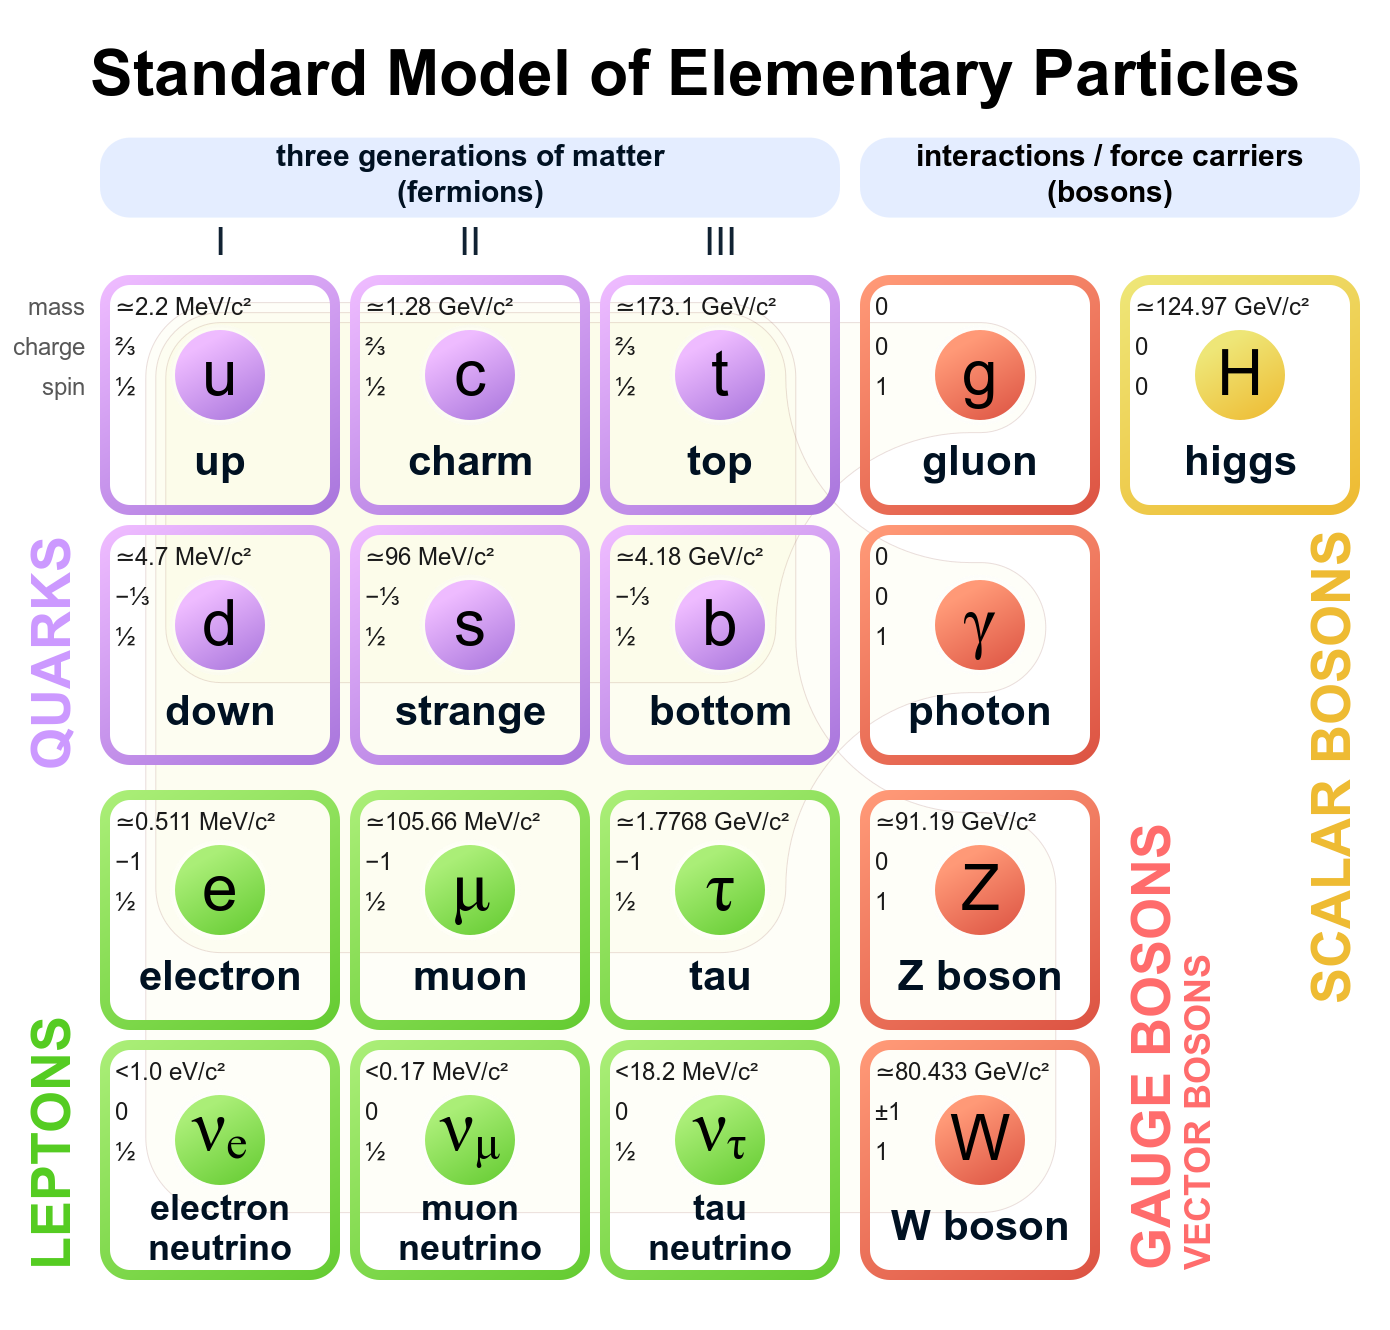
\includegraphics[scale=0.2]{figures/introduction/StandardModel.png}
    \caption{A diagram depicting the particles we currently believe are fundamental within the so-called ``Standard Model'' of particle physics.}
    \label{fig:standard_model}
\end{figure}
 It should be noted that all of the particles labeled as quarks and leptons -- collectively as ``fermions'' -- have corresponding anti-particles with opposite electric charge.
The equation that describes all of these particles and their interactions, often incorrectly\footnote[1]{It is ``incorrect'' because this is technically a Lagrangian density (i.e. Lagrangian per unit volume), but as it is usually integrated over all space the distinction is mostly irrelevant.} referred to as the ``Standard Model Lagrangian'', can be compactified into a relatively palatable form that can easily fit on a coffee cup like the one shown in Figure~\ref{fig:lagrangian_cup}.
\begin{figure}
    \centering
    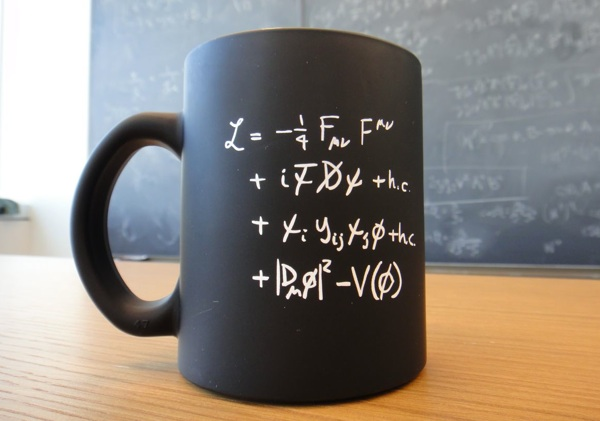
\includegraphics[scale=0.5]{figures/introduction/StandardModelCup.jpg}
    \caption{A coffee cup with the Standard Model Lagrangian density printed on its side. Please ignore the ``+ h.c.'' term following the $i\Bar{\psi}\slashed{D}\psi$, it is the result of a small lapse in judgement from the mug makers.}
    \label{fig:lagrangian_cup}
\end{figure}

While this equation may appear brief\footnote{Here ``brief'' is in the eye of the beholder, but certainly its brevity is misleading as even in the first line the $F_{\mu\nu}$ refers to three completely different gauge field tensors with their indices fully contracted...}, it can be used to completely describe three of the four fundamental forces of nature: 
\begin{enumerate}
    \item The Electromagnetic Force, which is responsible for the electrons pushing against each other to keep you from falling through your chair,
    \item The Weak Nuclear Force,  which is responsible for the initiating the nuclear fusion reactions that fuel our sun, and 
    \item The Strong Nuclear Force,  which is responsible for holding quarks and gluons together in bound stands known as hadrons, like the protons and neutrons that make up everyday matter.
\end{enumerate}
The only fundamental force missing from this list is the Gravitational Force, which is described by a completely separate set of equations\footnote{Specifically, the Einstein Field Equations, $G_{\mu\nu} + \Lambda g_{\mu\nu} = \kappa T_{\mu\nu}$, but this is the thesis of a particle physicist so gravity is taboo.}

Each of the three forces that are described within the Standard Model are mediated by different gauge bosons. For example, the electromagnetic force is mediated by the boson known as the photon, the weak nuclear force is mediated by the W and Z bosons, and the strong nuclear force is mediated by bosons known as gluons. 
In this thesis we will be primarily focusing on the Strong Nuclear Force, which acts solely on particles with color charge -- an intrinsic property of quarks and gluons. 
The ``color'' charges are red, green, and blue with antio

Even though each of the electromagnetic, weak and strong forces can be described using the Standard Model Lagrangian, the way in which they appear within the equation is not easy to determine.
For example, the electromagnetic force actually corresponds to line 1

% \chapter{Experimental Apparatus}
\label{ch:experiment}

As this thesis is focused on the physics of heavy-ion collisions, it stands to reason that the data analyzed in this thesis was gathered using the only detector along the LHC dedicated to studying such collisions: the ALICE detector. In this chapter, a brief synopsis of the LHC will be provided, followed by a much more detailed overview of the ALICE detector and its sub-detectors most relevant to this thesis.

\section{The LHC}
Located along the Swiss-French border near Geneva, Switzerland, the Large Hadron Collider (LHC)~\cite{LHC1, LHC2} is the largest particle accelerator on the planet. At a circumference of 27 kilometers, its tunnels lie almost 200 meters beneath the surface of the earth. Inside the tunnels are two high-energy particle beams pointing in opposite directions, with the beam pipes being kept inside of an ultra-high vacuum.
The particles inside the beam are guided by a multitude of superconducting magnets: 393 quadrupole magnets keep the beam focused, while 1232 dipole magnets bend the particles along the circular path. 
The beams are designed to collide at four intersection points along the LHC, each with a corresponding detector surrounding the collision points: 
\begin{enumerate}
\item ALICE~\cite{ALICE}, designed for investigating heavy-ion collisions
\item ATLAS~\cite{ATLAS}, designed for studying high-$p_{T}$ particles produced in pp collisions 
\item CMS~\cite{CMS},   designed for precise detection of muons
\item LHCb~\cite{LHCb}, designed for studying CP violations through measurements of B mesons at forward rapidity
\end{enumerate}
Note that ``designed for'' does not mean that these detectors are incapable of investigating other facets of particle collisions. For example, the ALICE detector is plenty capable for studying pp collisions\cite{ALICEpp1, ALICEpp2}, and the ATLAS and CMS detectors have been used to publish exciting results for heavy-ion collisions~\cite{CMSHeavy1, ATLASHeavy1}. A diagram of the LHC with these four intersection points can be seen in Figure \ref{fig:lhcring}.
\begin{figure}
    \centering
    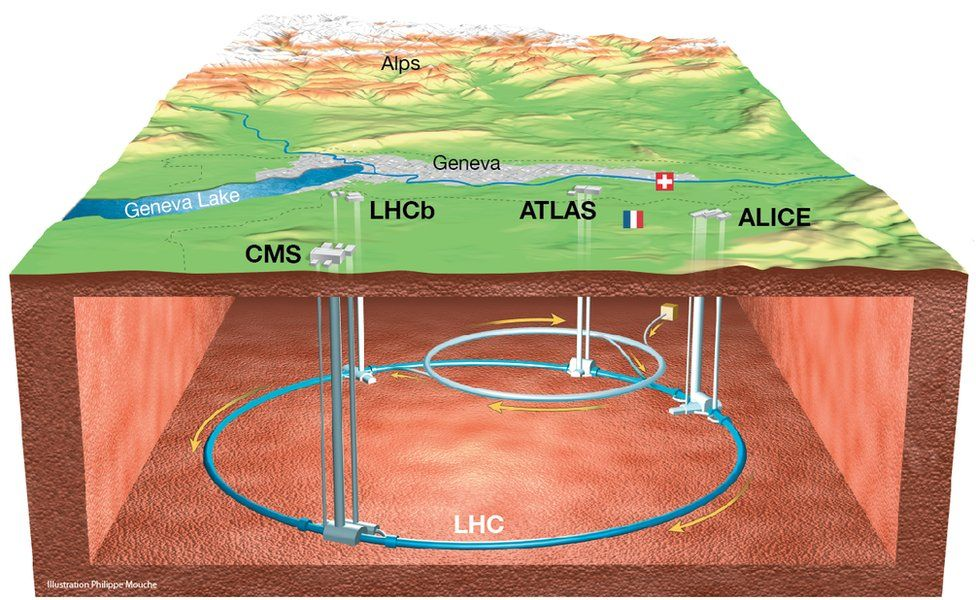
\includegraphics[width=0.8\textwidth]{figures/experiment/lhcring_illustration.jpeg}
    \caption{A diagram depicting the LHC with its various main detectors shown underground. Illustration by Philippe Mouche, taken from~\cite{LHCBBC}}
    \label{fig:lhcring}
\end{figure}
As of 2023, the highest center of mass energies achieved for each of the main collision systems (pp, p--Pb, Pb--Pb) are $\sqrt{s}$ = 13.6 TeV for pp, $\sqrt{s}$ = 7 TeV for p-Pb and $\sqrt{s}$ = 5.36 TeV for Pb--Pb. 

\section{The ALICE Detector}
The detector used by the A Large Ion Collider Experiment (ALICE) collaboration, unsurprisingly known as the ALICE detector, has the primary focus of investigating the physical properties of the strongly interacting quark-gluon plasma created during heavy-ion collisions.
Building the detector was a massive effort, requiring the help from over 1000 people from 105 institutes in 30 different countries. 
The detector itself is also massive, weighing in at around 10,000 tons, and spanning 26 meters in length with a 16-meter height and width.
It is composed of 18 sub-detector systems, all of which work together to help reconstruct the event.
A diagram of the detector with its corresponding sub-detector systems can be seen in Figure \ref{fig:alice_detector}.
\begin{figure}
    \centering
    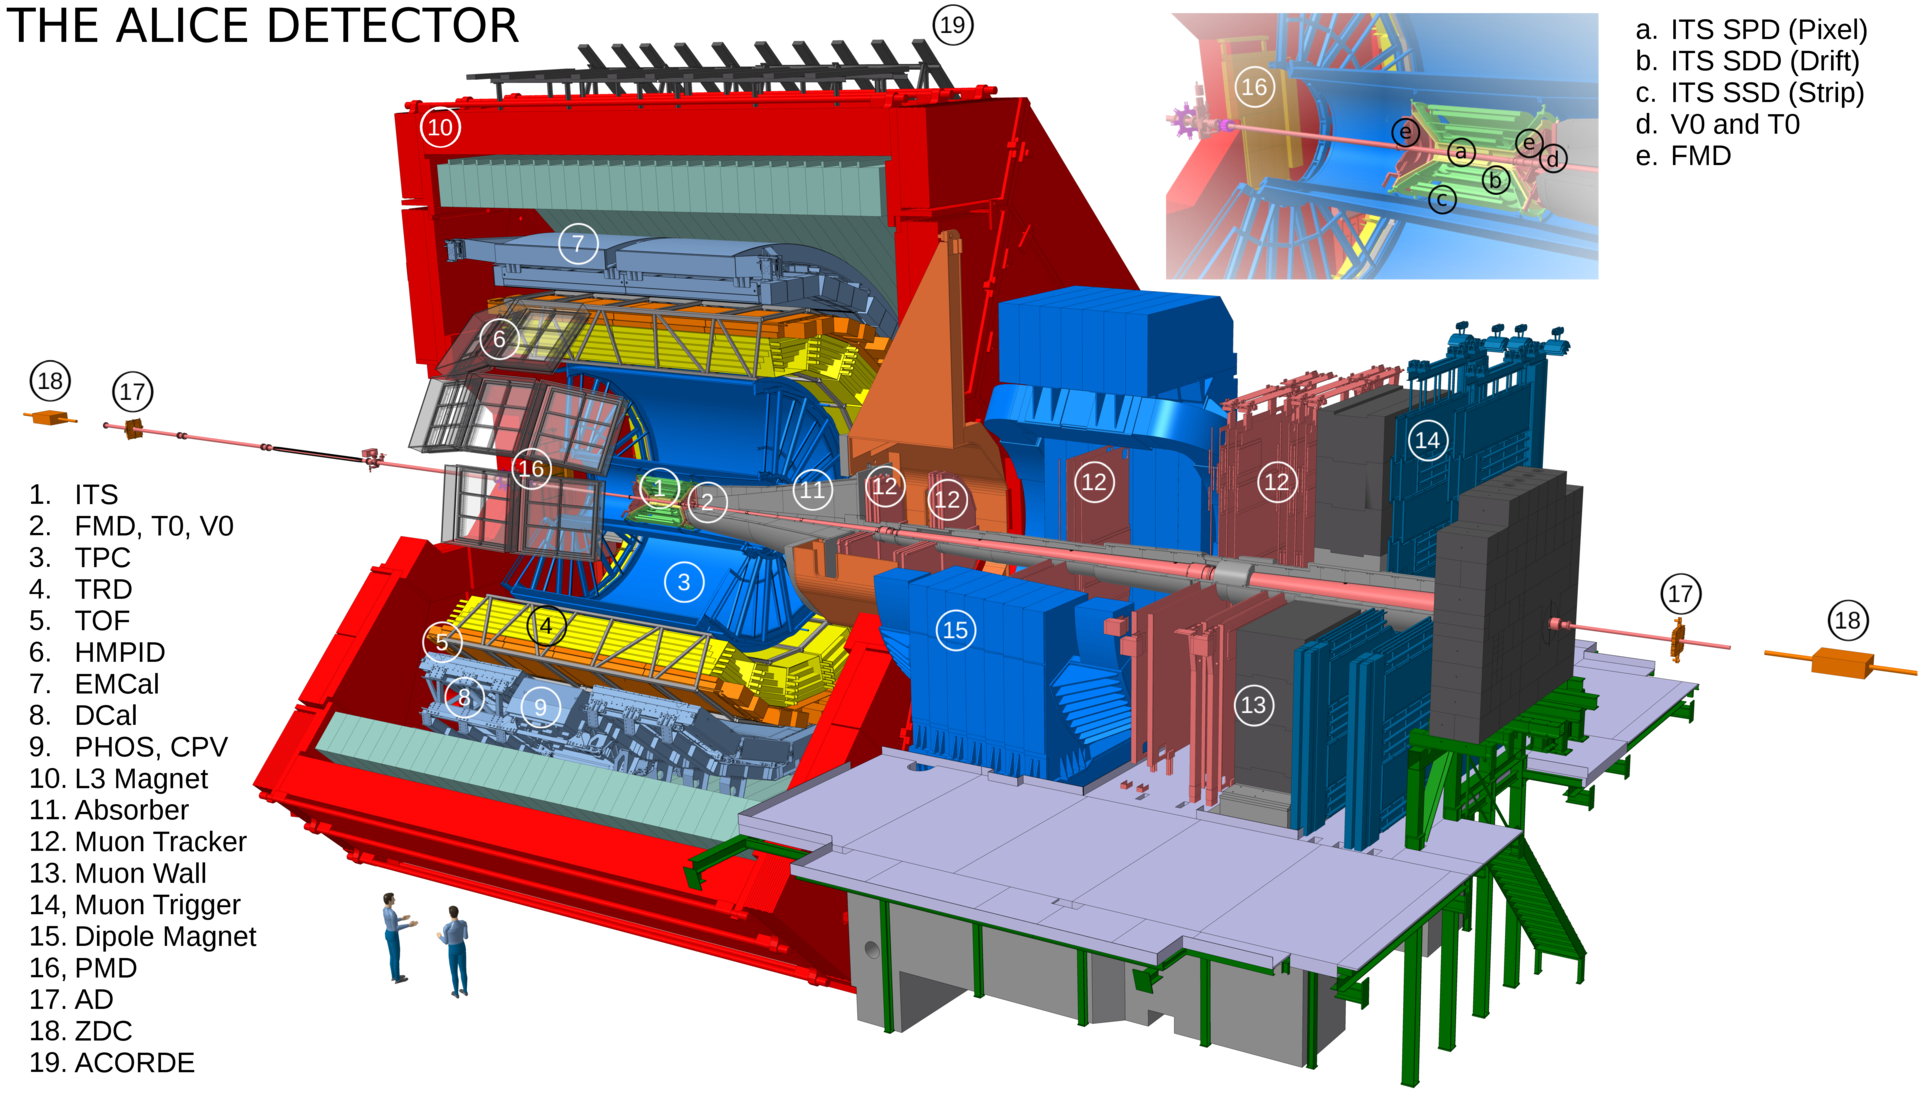
\includegraphics[width=0.8\textwidth]{figures/experiment/ALICE_detector_schematic.png}
    \caption{A 3-D schematic of the ALICE detector, with labels for all of the sub-detectors, taken from~\cite{ALICEDiagram}. Note the humans-for-scale in the bottom left of the diagram.}
    \label{fig:alice_detector}
\end{figure}
As the primary focus of the ALICE detector is to study heavy-ion collisions, all of its components must work together to reconstruct very high multiplicity events. The components most relevant to this thesis will be discussed in the following sections.

\subsection{Detector coordinates}
Before discussing the components of the ALICE detector, it is important to first define a coordinate system suitable for describing the geometry of the detector and the collisions within. As the ALICE detector is a giant cylinder, the most pragmatuc choice is cylindrical coordinates, with the $z$-axis pointing along the beam line. An example of this cylindrical coordinate system is shown in Figure \ref{fig:detector coordinates}. The plane defined by the x- and y-axes is often referred to as the \textbf{transverse plane}, with the angle $\varphi$ referred to as the \textbf{azimuthal angle}.

\begin{figure}
    \centering
    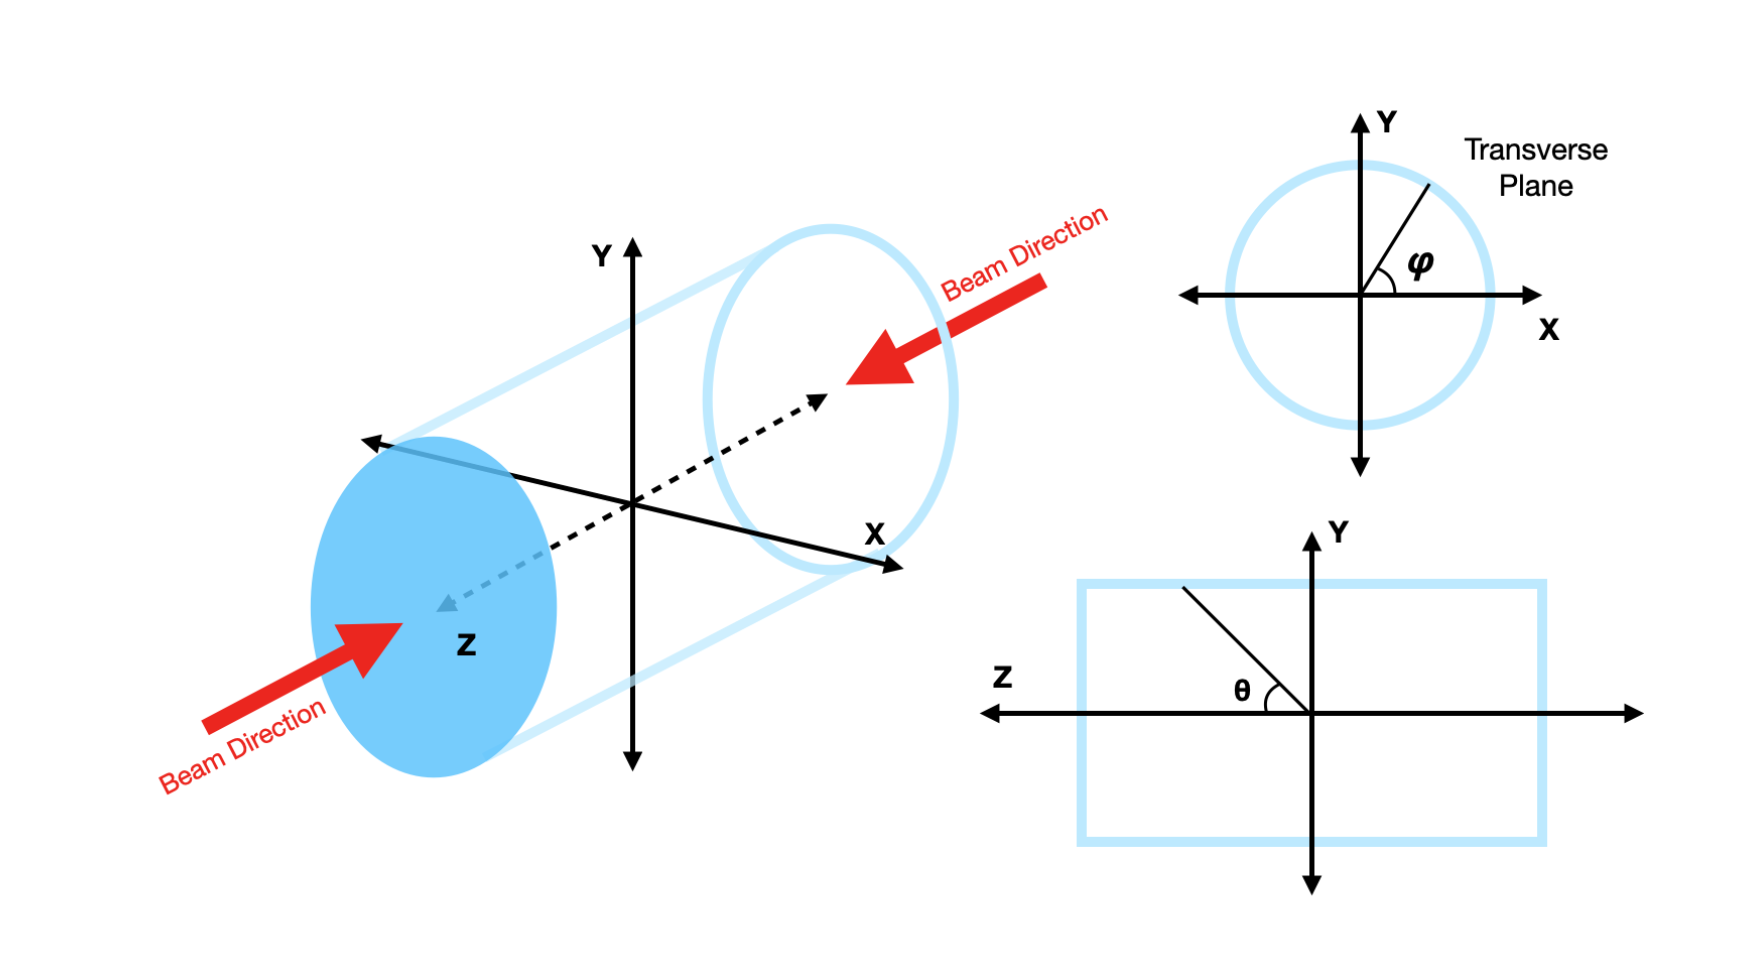
\includegraphics[width=0.8\textwidth]{figures/experiment/detector_coordinates.png}
    \caption{A diagram showing the cylindrical coordinate system used to describe the ALICE detector.}
    \label{fig:detector coordinates}
\end{figure}

Unfortunately, collisions within the ALICE detector involve particles moving at relativistic speeds in the beam (z) direction. Thus the polar angle $\theta$ is not particularly useful, as it is not Lorentz invariant. Instead, a more useful quantity is the rapidity $y$, which can be defined as
\begin{equation}
    y = \frac{1}{2} \ln \left( \frac{E + p_{z}}{E - p_{z}} \right),
\end{equation}
where $E$ is the energy of the thing being measured and $p_{z}$ is the momentum in the z-direction. This quantity is preferable to $\theta$ as differences in rapidity are invariant under Lorentz boosts along the z-axis. This follows directly from the fact that rapidity is often defined in terms of such boosts,
\begin{equation}
    \left(\begin{array}{c}
        c t^{\prime} \\
        z^{\prime}
        \end{array}\right)=\left(\begin{array}{cc}
        \cosh y & -\sinh y \\
        -\sinh y & \cosh y
        \end{array}\right)\left(\begin{array}{c}
        c t \\
        z
        \end{array}\right) \equiv \Lambda(y)\left(\begin{array}{c}
        c t \\
        z
        \end{array}\right).
\end{equation}
It can be shown\footnote{Using various properties of the hyperbolic trigonometric functions.} that $\Lambda(y)$ obeys
\begin{equation}
    \Lambda(y_1 + y_2) = \Lambda(y_1)\Lambda(y_2),
\end{equation}
which in turn gives a rapidity addition rule for reference frames A, B and C moving along the z-axis,
\begin{equation}
    y_{AC} = y_{AB} + y_{BC}.
\end{equation}
Now suppose reference frame A is the lab (stationary) frame, and reference frames B and C correspond to two different particles. The above equation can then be written as
\begin{equation}
    y_{AC} - y_{AB} = y_{BC} = y_{A'B} - y_{A'C},
\end{equation}
where $A'$ can be \textit{any} reference frame. In other words, the difference in rapidity between any two particles does not depend on the reference frame the measurement is made in. Another consequence of this property is that rapidity distributions of particles do not change shape in different reference frames: they only get shifted along the rapidity axis.

However, the total energy of a given particle is often not known, and thus rapidity is replaced by the more experiment-friendly \textbf{pseudorapidity}, 
\begin{equation}
    \eta = \frac{1}{2} \ln \left( \frac{|\vec{p}| + p_{z}}{|\vec{p}| - p_{z}} \right) 
        = -\ln \left( \tan \frac{\theta}{2} \right),
\end{equation}
where $\theta$ is the aforementioned polar angle. This quantity can be directly measured by experiment, at the expense of losing a small amount of Lorentz invariance: the \textit{pseudo} part of pseudorapidity comes from the idea that at very high momentum ($p >> m$), the rapidity and pseudorapidity are approximately equal.

\section{The Inner Tracking System}
\label{sec:its}

The Inner Tracking System (ITS)~\cite{ITS} is the inner most component of the ALICE detector, lying closest to the beam pipe. It is composed of six cylindrical layers of silicon detectors that are coaxial with the beam pipe and cover the pseudorapidity range $|\eta| \leq 0.9$. The distance from the beam line varies from 3.9 cm for the first layer to 43 cm for the sixth layer. A diagram of the ITS can be seen in Figure~\ref{fig:its_schematic}. Because of its proximity to the interaction point, the ITS is invaluable for reconstructing both primary and secondary vertices and enhancing the tracking capabilities of the ALICE detector near the interaction point. Moreover, the ITS can also track particles that are not detected or missed by the external barrel detector due to acceptance limitations and momentum cutoff. 

\begin{figure}
    \centering
    \includegraphics[width=0.8\textwidth]{figures/experiment/its_diagram.png}
    \caption{A schematic of the ITS showing the six layers of silicon detectors, taken from~\cite{ITSDiagram}.}
    \label{fig:its_schematic}
\end{figure}

The ITS uses different types of silicon detectors for each layer, which will be briefly discussed in the following sections.

\subsection{Layers 1 and 2}

The first and second layers of the ITS are composed of \textbf{Silicon Pixel Detectors} (SPD)~\cite{ITSSPD}. The SPD inner and outer barrel layers have radii of 3.9 cm and 7.6 cm, respectively. The pseudorapidity coverage is $|\eta| < 1.95$, the highest of all the ITS detectors. The SPD is segmented into 10 sectors which each cover 36 degrees in azimuth. Each of these sectors contains 12 modules--caled half-staves--which themselves consist of 10 silicon pixel chips. These chips are 13.68 mm $\times$ 15.58 mm in size and contain 8192 pixels each, corresponding to a pixel size of 425 $\mu$m $\times$ 50 $\mu$m. This small pixel size gives rise to a very low occupancy ($<2$\%) for even the most central Pb--Pb collisions.  As the track densities in the innermost layers are very high (up to 100 tracks/cm$^2$ for central Pb--Pb collisions), the SPD has a very high granularity in order to keep the occupancy low. The SPD is also used to generate the L0 trigger signal, which is used to trigger the readout of the TPC and TRD.

\subsection{Layers 3 and 4}
The middle two layers of the ITS are made up of \textbf{Silicon Drift Detectors} (SDD)\cite{ITSSDD}. These layers extend from an inner radius of 14 cm to an outer radius of 24 cm, and cover the pseudorapidity range $|\eta| < 0.9$. There are 260 large area (7.02 $\times$ 7.53 cm$^2$) SSD modules in total, which are split into two drift regions. As an ionizing particle passes through the drift regions, the resulting electrons \textit{drift} into the collection anodes, which are at the ends of the drift regions and are connected to the frontend readout electronics. This separates the SPD and the SDD in a fundamental way--the data from the SDD is analog, and depends very much on how many electrons were ``knocked loose'' during ionization. The SPD, on the other hand, is digital, and only registers a hit (1) if a charged particle passes through the pixel. This analog information can be used to help identify the ionizing particle species using the Bethe-Bloch formula, which will be discussed in more detail in Section~\ref{sec:tpc}. Furthermore, there are MOS charge injectors~\cite{MOSCharge} connected to the cathodes in the drift region, which provide precise timing information to compute the electron drift velocity. This velocity is needed to precisely measure the location of the initial ionizing particle along the direction of the applied electric field. As the track density in the middle layers is lower than in the innermost layers, the SSD has a coarser granularity than the SPD.

\subsection{Layers 5 and 6}
The last two layers of the ITS are \textbf{Silicon Strip Detectors} (SSD)~\cite{ITSSSD}, which have an inner radius of 38 cm and an outer radius of 43 cm. The SSD covers the pseudorapidity range $|\eta| < 0.9$, and is composed of 1698 modules in total. These modules are a 1536-strip double-sided silicon sensor, with each strip connected to the front-end readout electronics. Similar to the SDD, the SSD collects electrons generated when the ionizing particle travels through the silicon--though the drift distance is \textit{much} smaller (300 microns for the SSD vs. 70.2 mm for the SDD). The SSD provides two dimensional measurements of the ionizing particle's position with a 20 micron resolution in the $r\varphi$ direction. The SSD also captures an analog signal, and is therefore used to help identify the ionizing particle species.


\subsection{ITS Upgrade}
During the long shutdown (LS2) from December 2018 to June 2022, the LHC underwent a fairly substantial upgrade to allow for higher beam energies and luminosities. The luminosity increase from Run 2 (before LS2) to Run 3 (after LS2) was substantial, from 12 inverse femtobarns before the shutdown to well over 200 inverse femtobarns after starting up again~\cite{LHCUpgrade}. As such, the ALICE detector needed to undergo quite a few upgrades to keep up with the increased collision rates. In terms of pure hardware upgrades, only three detectors were affected, namely
\begin{itemize}
    \item the Time Projection Chamber (TPC)~\cite{TPCUpgrade},
    \item the Muon Forward Tracker (MFT)~\cite{MFTUpgrade}, and
    \item the ITS~\cite{ITSUpgrade}.
\end{itemize}
The TPC and MFT upgrades will not be summarized in this thesis\footnote{The author of this thesis was intimately involved with the ITS upgrade, and thus would be unable to provide a fair and unbiased description of the TPC and MFT upgrades.}, but some key features of the ITS upgrade will be discussed in the following sections.

\subsubsection{Motivation for the ITS upgrade}
As mentioned previously, the increased collision rates associated with the higher luminosity LHC beam necessitated an upgrade to the ITS. Previously, the readout rate for the ITS was 1 kHz for both pp and Pb--Pb collisions. The upgraded ITS, on the other hand, is able to readout at 100 kHz for Pb--Pb and 200 kHz for pp collisions, drastically increasing the amount of possible data to be taken over the course of Run 3. The upgraded ITS also has a much finer impact parameter resolution than the previous ITS, improving by a factor of 3 in the $r\phi$ coordinate and by a factor of 5 in the $z$ coordinate. This improved resolution is crucial for the ALICE physics program, as it allows for the reconstruction of more secondary vertices--like those from the decay of a B meson; this was previously not possible with the old detector. The tracking efficiency at lower $p_T$ was also improved, thanks to a strong reduction in the material budget (from 1.14\% $X_0$ to 0.35\% $X_0$).


\subsubsection{Hardware overview}
The upgraded ITS consists of seven layers of silicon detectors, as shown in Figure~\ref{fig:its_upgrade_schematic}. There are a total of 192 \textit{staves}--rows of silicon chips--which cover a total area of 10 square meters. Each chip is of the same technology, which will be discussed in more detail in the next section. The first three layers form the Inner Barrel (IB), and contain 48 staves of 27 cm length. The remaining layers are referred to as the Outer Barrel (OB). The OB is further separated into the Middle Layers (MLs) and Outer Layers (OLs), which correspond to the 4-5th and 6-7th layers, respectively. The MLs each have 54 staves of length 84 cm, and the OLs have 90 staves of 150 cm. The grouping of the layers into the IB and OB has ramifications for the hardware testing procedure, which is described in Section~\ref{sec:hardware_testing}.

\begin{figure}
    \centering
    \includegraphics[width=0.8\textwidth]{figures/experiment/its_upgrade_schematic.png}
    \caption{A schematic of the ITS upgrade, showing the seven layers of silicon detectors.}
    \label{fig:its_upgrade_schematic}
\end{figure}


\subsubsection{The ALPIDE chip}
The star of the show for the ITS upgrade is the introduction of a new silicon pixel chip: the ALPIDE~\cite{ALPIDE}. The ALPIDE chip is a CMOS Monolithic Active Pixel Sensor (MAPS) that has a few advantages over its predecessors (e.g. the SPD):
\begin{itemize}
    \item Thanks to a deep p-well, complex logic at the pixel level can be employed. This deeper p-well prevents the n-well PMOS part of the CMOS transistor from collecting unwanted electrons (which are intended for the collection electrodes)
    \item These CMOS transistors allow for complicated in-pixel circuitry, which (when coupled with the priority encoder) \textit{drastically} reduces the data rate by only sending the addresses of ``hit'' pixels to the frontend electronics
\end{itemize}
Each chip is $15\times30$ mm$^2$, and contains over half a million pixels (512 rows, 1024 columns). This corresponds to a spatial resolution of 5 microns, which is much better than the SPD of the old ITS (around 50 microns in $r\varphi$). A diagram of the cross section of an ALPIDE (or more generally a MAPS) pixel can be seen in Figure~\ref{fig:alpide_diagram}. In this diagram, a charged hadron flies through the chip, generating many electron-hole pairs. The electrons are guided to the n-well diode, which ultimately collects the electrons and generates a signal. The CMOS transistors (NMOS and PMOS transistors) are vitally important for the pixel-level logic. Without the deep p-well to protect the PMOS's n-well from wandering electrons, the PMOS (and therefore the CMOS) transistors would be rendered useless.

\begin{figure}
    \centering
    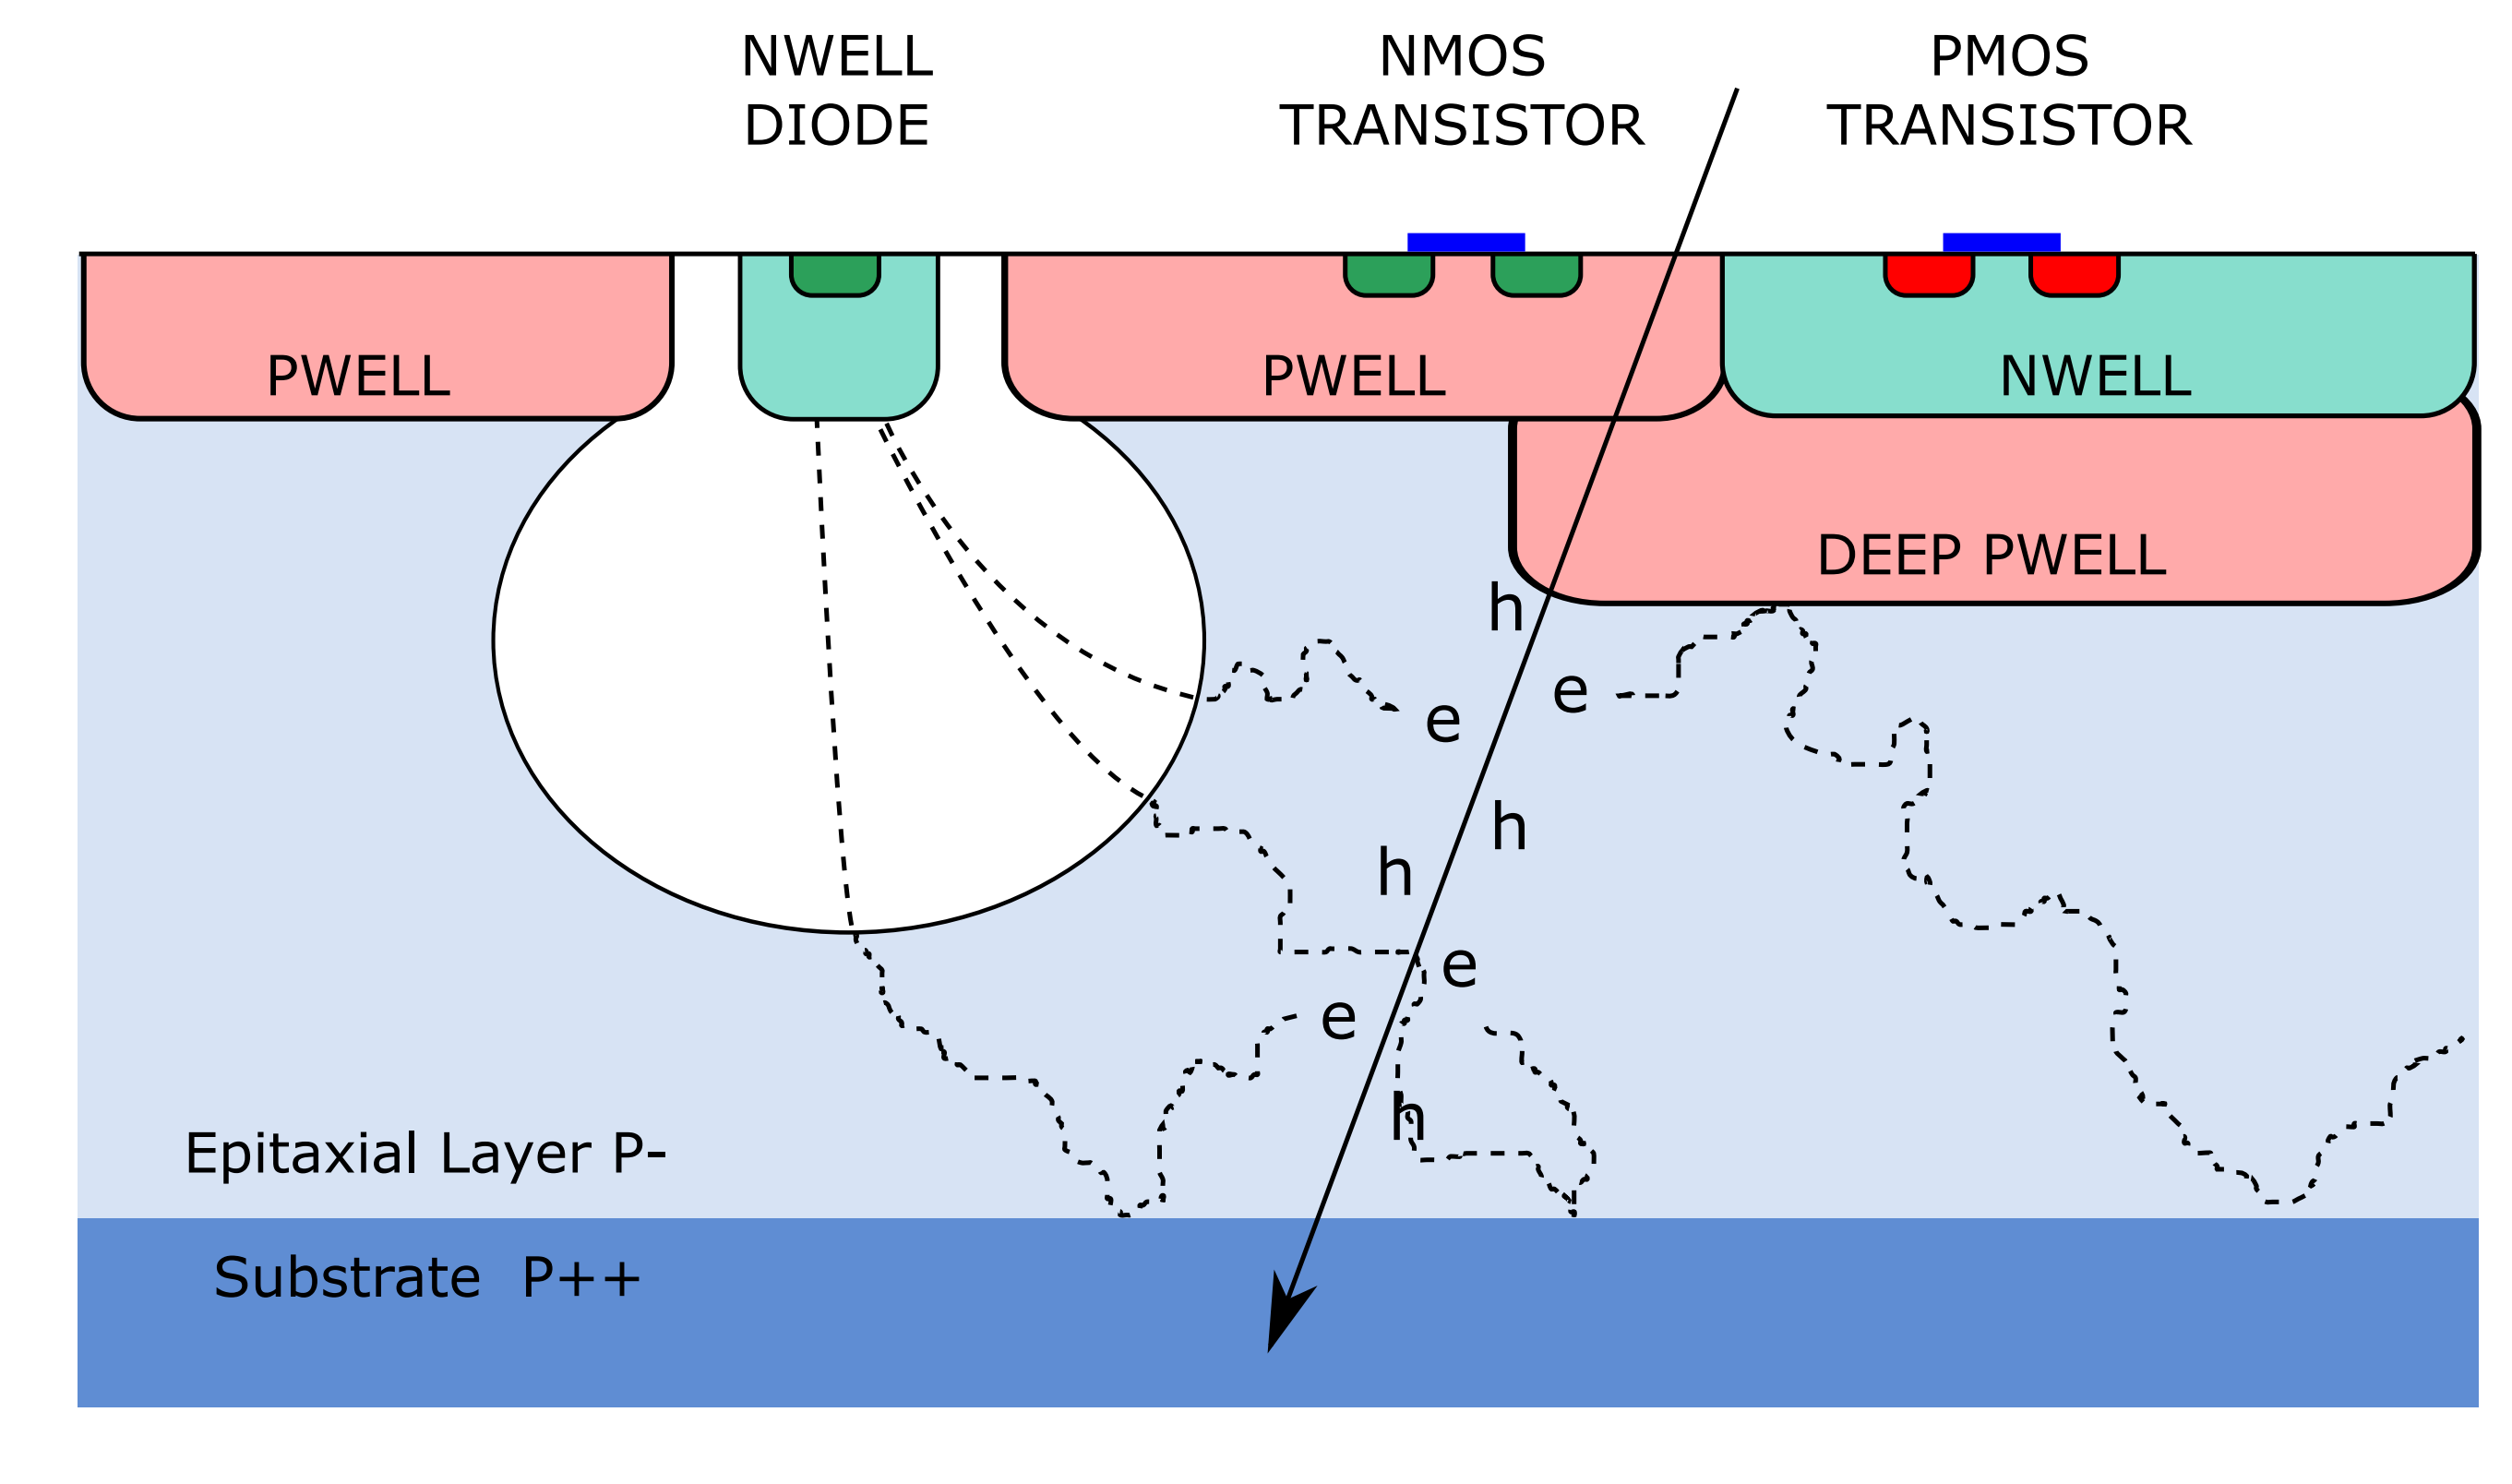
\includegraphics[width=0.8\textwidth]{figures/experiment/alpide_cross.png}
    \caption{A diagram showing the basic operating principle of a MAPS pixel.}
    \label{fig:alpide_diagram}
\end{figure}

These CMOS transistors work together to form the logic within the pixel, shown as a block diagram in Figure ~\ref{fig:alpide_l}. First, the collection diode sends a signal \textit{SUB}, which comes in the form of a large voltage drop in a very short ($\approx 10$ ns) time, followed by a slow requilibration. The \textit{VPULSE} signal is used for testing purposes, where a ``fake'' charge can be sent to the capacitor, generating a similar signal to the collection diode. The resulting \textit{PIX\_IN} signal is sent to an amplifier $+$ signal shaper, and then to a discriminator with threshold \textit{THR}. If the amplified signal is less than the threshold, no \textit{OUT\_D} signal is generated. The digital \textit{OUT\_D} signal is then sent into a simple AND gate, where the other input signal is the digital \textit{STROBE}. This strobing window is ultimately initialized by a trigger signal, and its width is configurable. If the \textit{OUT\_D} signal is high during the strobing window, then one of the three hit storage registers is ``latched'' (i.e. set to one). Also included in the pixel logic is a masking register, which masks the pixel during readout when hot. 

The priority encoder (which physically lies between two columns of pixels) sequentially provides the addresses of the latched pixels to the frontend electronics on the chip. An important feature of the on-pixel electronics and priority encoder is the lack of a clock: this means that there is no activity if there are no hits. In other words, the ALPIDE chip is not sending a bunch of useless 0's to the readout electronics, saving precious bandwidth.

\begin{figure}
    \centering
    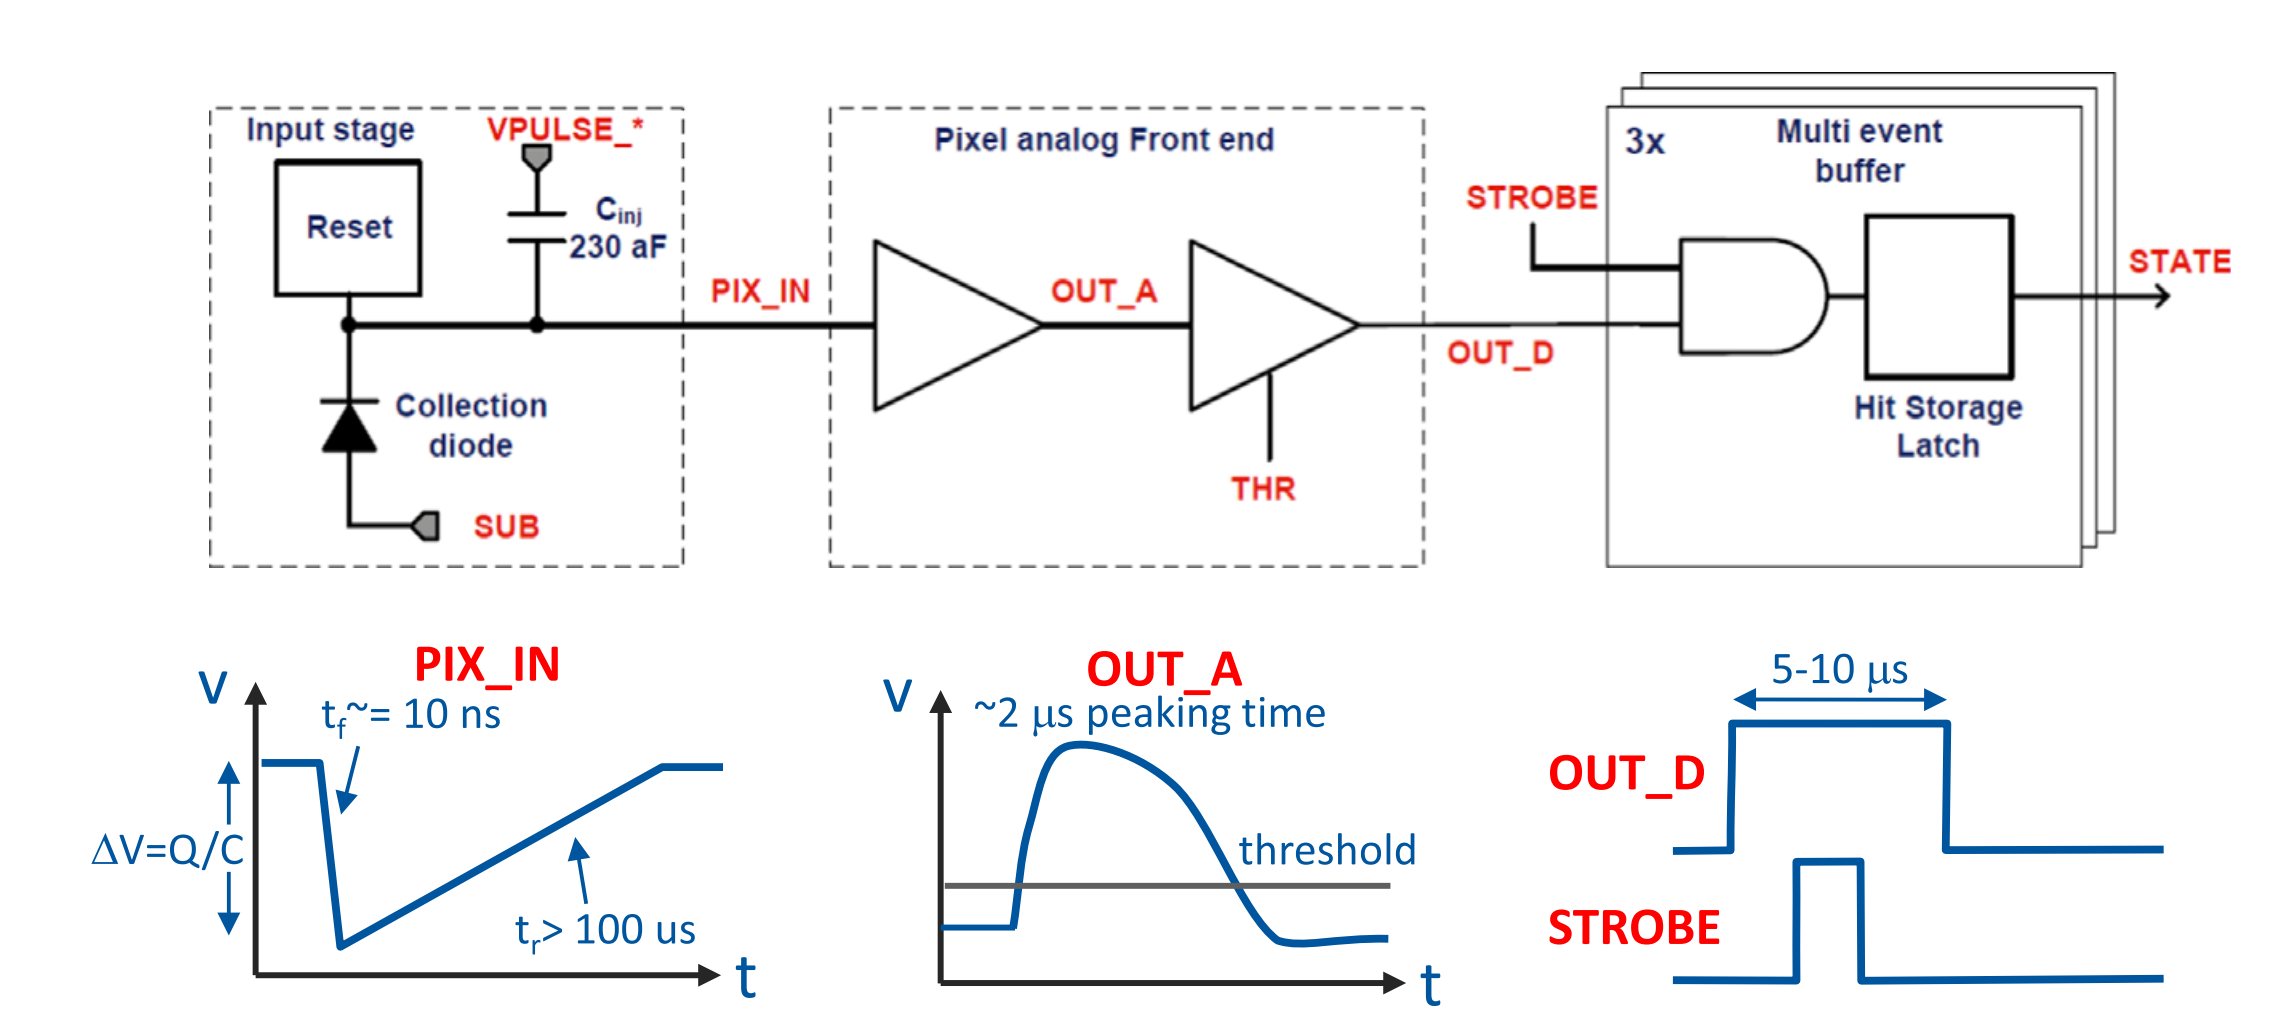
\includegraphics[width=1.0\textwidth]{figures/experiment/alpide_logic.png}
    \caption{A block diagram showing the logic embedded on top of a single ALPIDE pixel.}
    \label{fig:alpide_l}
\end{figure}

\subsubsection{Characterizing the chips for commissioning}
\label{sec:hardware_testing}

Each ALPIDE chip has over 500,000 pixels, each with their own circuit logic. Excluding issues with the frontend electronics on the chip, that is still \textit{over} 500,000 possible points of failure. As such, the chips were thoroughly tested to determine if they are worthy of being installed in the ITS. There are three main tests that were performed on each chip:
\begin{enumerate}
    \item \textbf{Fake hit rate}: All pixels are unmasked, and a \textit{STROBE} signal is repeatedly sent to each pixel. As the \textit{THR} signal should prevent any hits from being registered, any latched pixels are considered ``fake hits''.
    \item \textbf{Threshold scan}: A predetermined amount of charge is injected into each pixel via the \textit{VPULSE} signal, and the \textit{THR} signal is varied. There should be a clear threshold where every pixel registers a hit, and vice-versa.
    \item \textbf{Readout tests}: Either a digital signal (by writing the hit storage register) or an analog signal (by injecting charge into the capacitor) pattern is sent to the entire chip, and then the corresponding output is read out. The resulting output should be the same as the input, like the example shown in Figure~\ref{fig:ut_alpide}.
\end{enumerate}

\begin{figure}
    \centering
    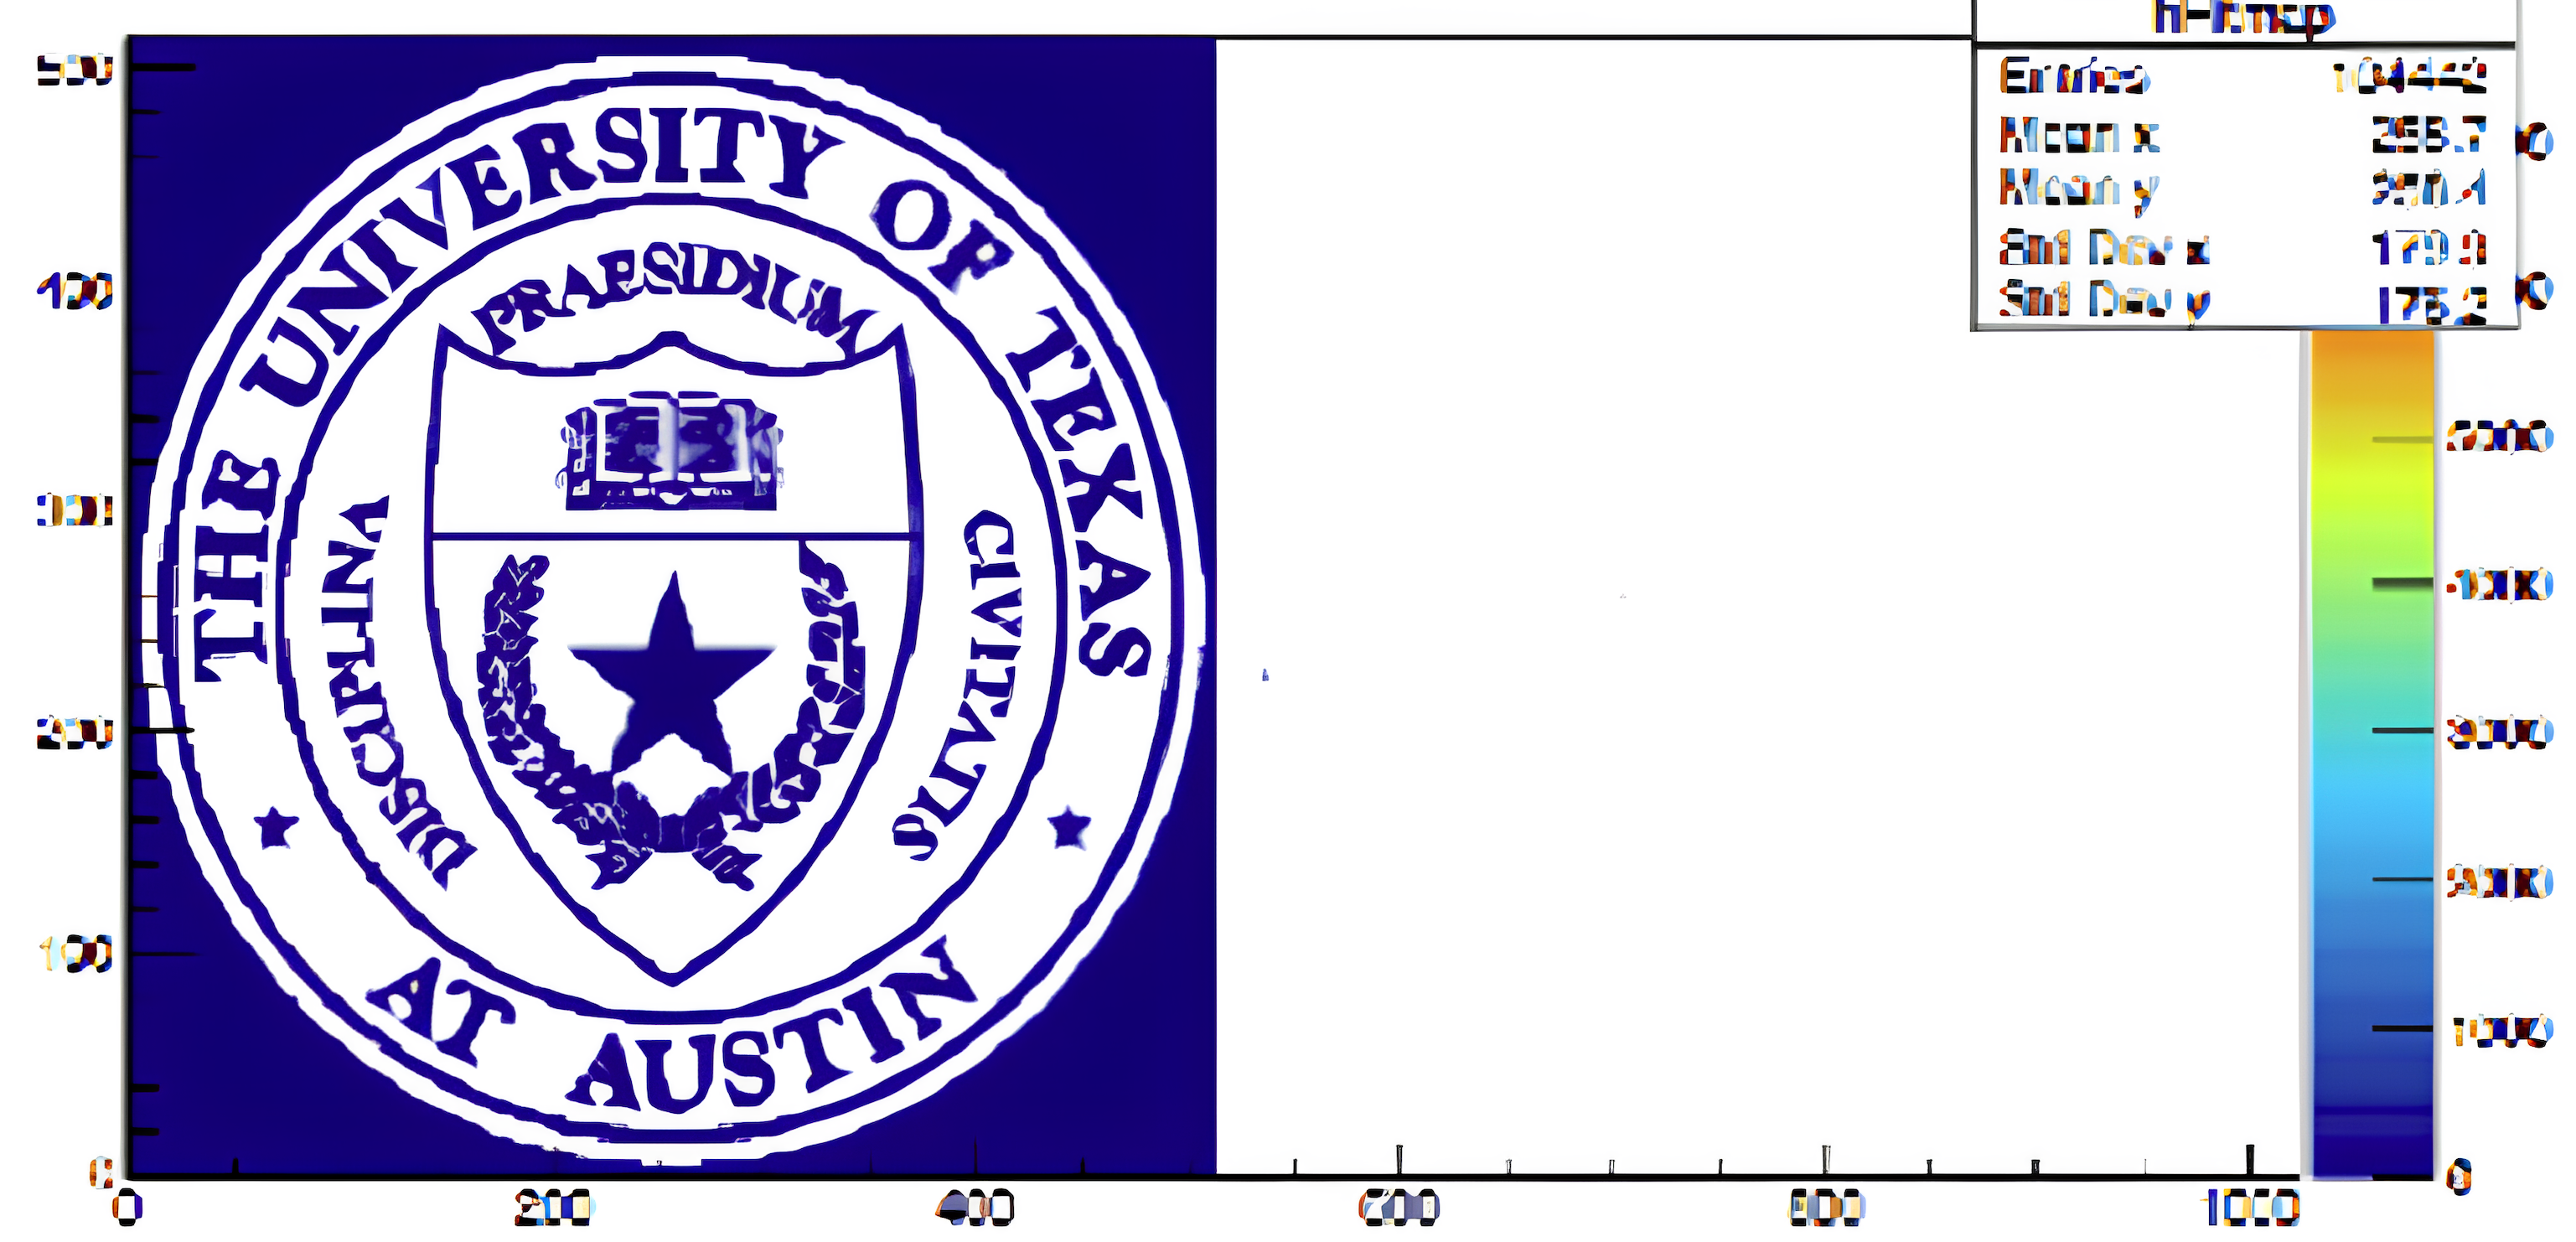
\includegraphics[width=0.9\textwidth]{figures/experiment/ut_alpide.png}
    \caption{The signal that was read out from the ALPIDE chip after sending an extremely technical digital input pattern.}
    \label{fig:ut_alpide}
\end{figure}

These tests were run on the ALPIDE software, which is a graphical user interface (GUI) that allows for easy communication with the chips. The resulting output of the tests was simply one of four options, which are summarized in Table~\ref{tab:chip_medals}. This medal system was used to determine where the chip should be installed within the detector. If a chip was GOLD, it was reserved for the IB. If the chip was SILVER, it could be installed in either the MLs or the OLs. If the chip was BRONZE, it could only be installed in the OLs. Finally, if the chip FAILed the tests, it was discarded\footnote{Sent to the poor souls developing the ALPIDE software.}. Further characterization was done at the stave level to determine where within the IB or OB a particular stave should be installed.

\begin{table}
    \centering
    \caption{A summary of the medal system used to determine where a particular chip should be installed. Note that while 99\% \textit{seems} strict, it corresponds to over 5000 misbehaving pixels.}
    \begin{tabular}{|c|c|}
        \hline
        \textbf{Medal} & \textbf{\% of good pixels} \\
        \hline
        GOLD & 99.99\% \\
        SILVER & 99.67\% \\
        BRONZE & 99.00\% \\
        FAIL &  $<$ 99.00\% \\
        \hline
    \end{tabular}
    \label{tab:chip_medals}
\end{table}

\subsubsection{The readout unit}
Another large overhaul for the ITS upgrade was a complete redesign of the readout system, from chip to DAQ. A schematic of the new readout system can be seen in Figure~\ref{fig:its_readout}. Each detector stave is connected to a \textbf{readout unit} (RU) via a relatively long copper data cable. A single RU has a lot of responsibilities, including
\begin{itemize}
    \item communicating with the power board so it can properly power the chips,
    \item receiving the trigger information from the Central Trigger Processor (CTP) and sending it to the chips (which generates the \textit{STROBE} signal discussed above),
    \item receiving \textit{all} of the data from the chips on the stave, which each have their own 1.2 Gbps link (for the IB chips, the OB chips share a 400 Mbps link in groups of seven), and
    \item sending the readout data from the chips to the Common Readout Unit (CRU), 
\end{itemize}
all while being in a highly radiative environment (only 6-8 meters away from the detector). 

\begin{figure}[h]
    \centering
    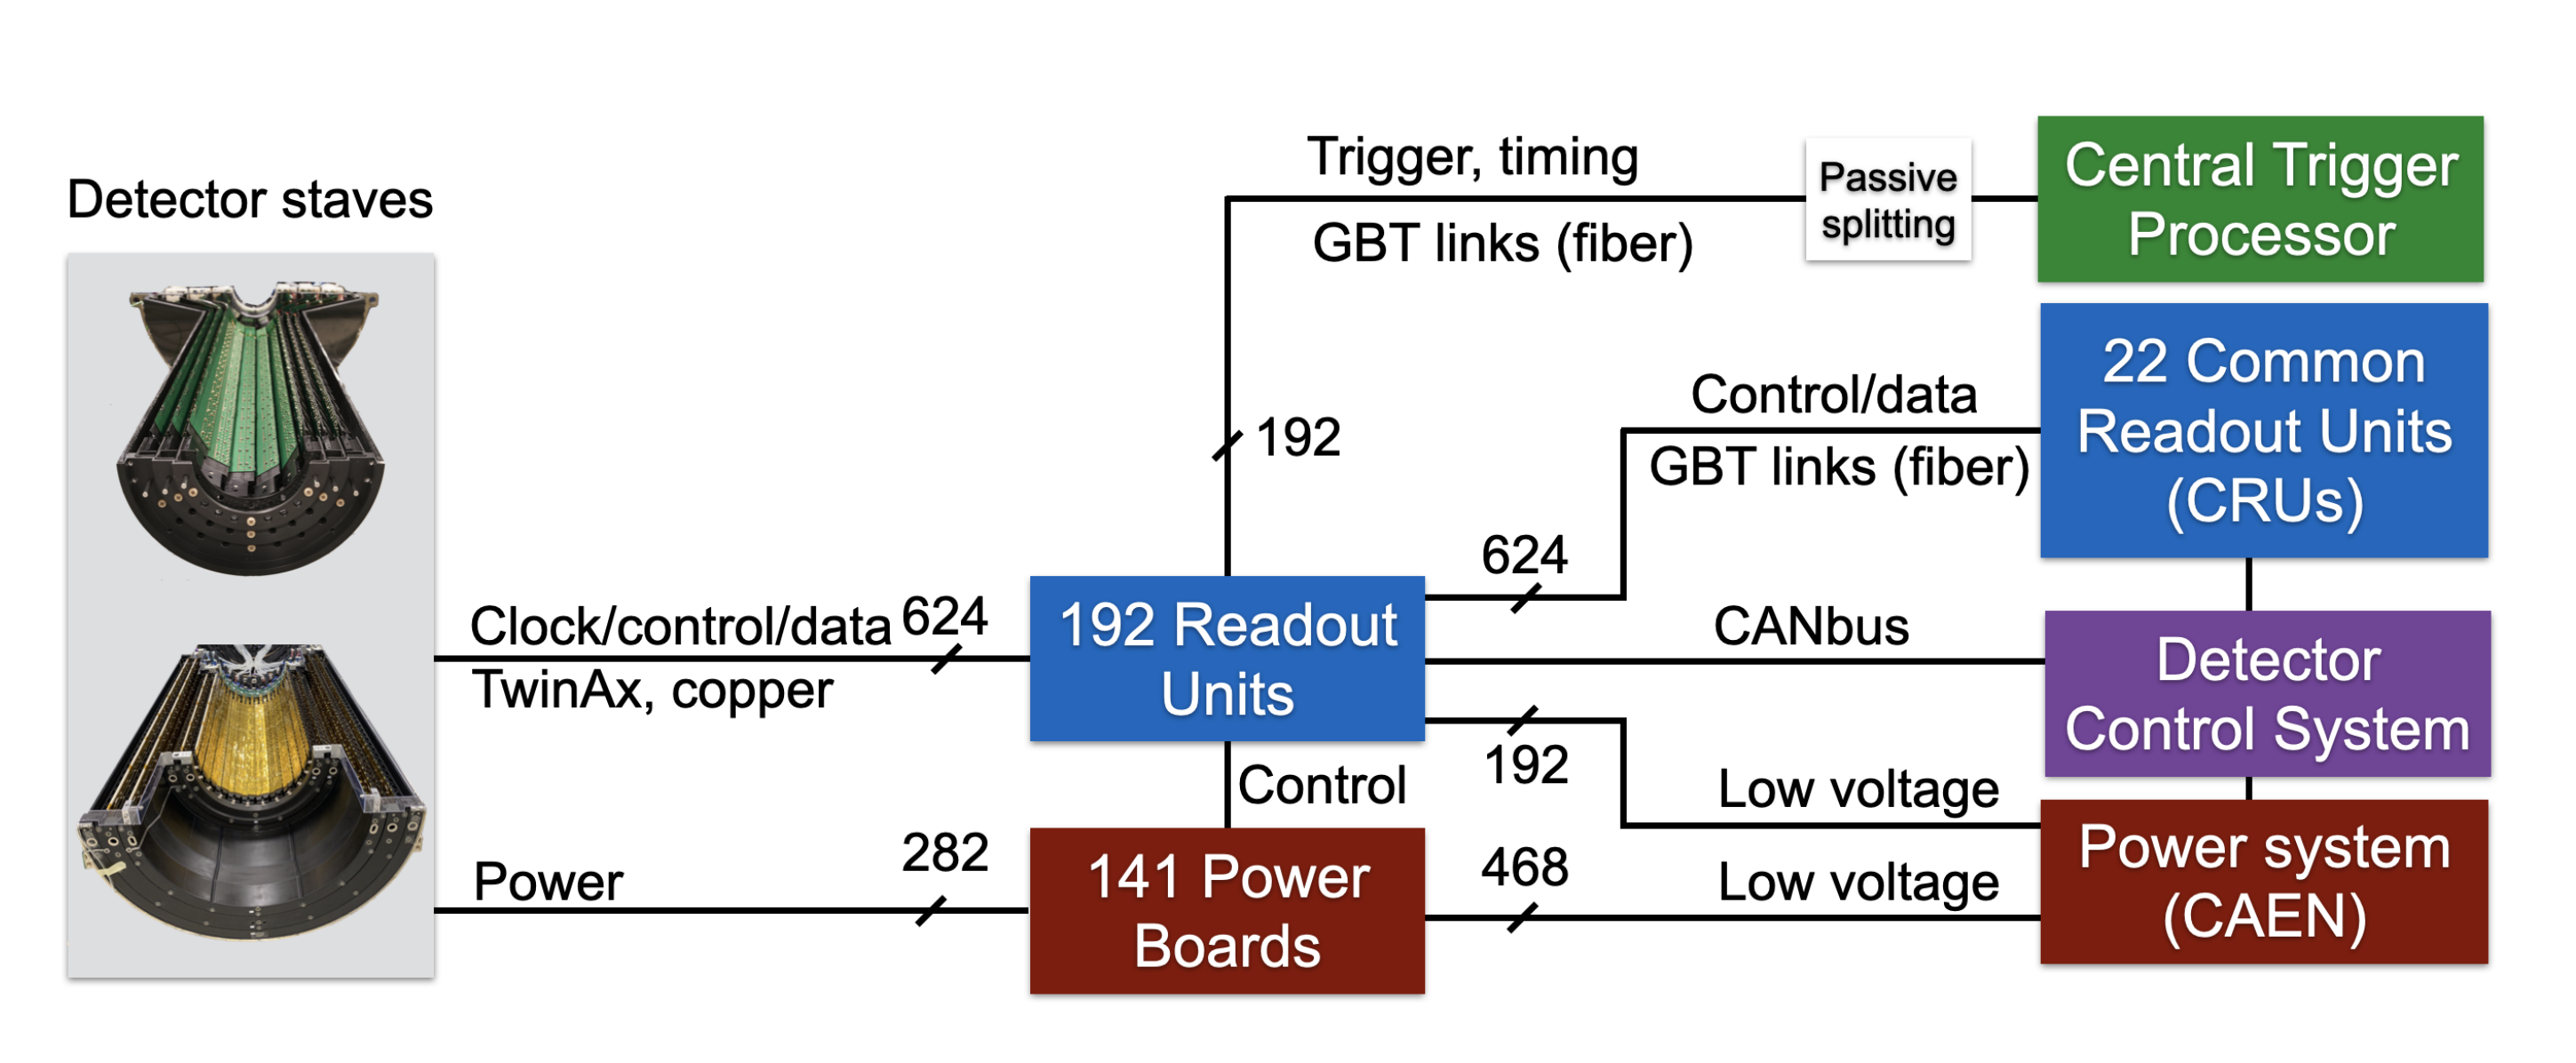
\includegraphics[width=0.9\textwidth]{figures/experiment/its_readout.png}
    \caption{A schematic of the ITS readout system, showing the various components of the system.}
    \label{fig:its_readout}
\end{figure}

These responsibilities are mostly handled by two on-board field-programmable gate arrays (FPGAs): an SRAM FPGA for actually handling all of the aforementioned data transfer between the various components, and a flash FPGA for ensuring that the SRAM FPGA does not misbehave in the radiative environment. The SRAM FPGA continuously scrubs the flash FPGA to ensure that it has not been misconfigured due to a radiation upset. If it has, the SRAM FPGA will reconfigure it using the ``golden image'' of the SRAM firmware stored in the flash memory of the flash FPGA (hence the name). Even still, the important modules of the SRAM FPGA are triplicated, meaning that if one module is subject to a radiation upset, the other two can outvote it. An image of the RU at the University of Texas at Austin can be seen in Figure~\ref{fig:ut_ru}.

\begin{figure}
    \centering
    \includegraphics[width=0.9\textwidth]{figures/experiment/ut_ru.png}
    \caption{A picture of a readout unit in its (not-so) natural habitat at the University of Texas at Austin. The heat sink and fan are covering the main SRAM FPGA, and to its north-east is the flash FPGA.}
    \label{fig:ut_ru}
\end{figure}

\section{The Time Projection Chamber}
\label{sec:tpc}
The largest component of the ALICE detector is known as the Time Projection Chamber (TPC)~\cite{TPC1, TPC2}. The TPC is a gas-filled volume with an 85 cm inner radius, a 250 cm outer radius, and a five meter length along the beam axis. This corresponds to an active volume of around 90 cubic meters, all of which is filled with a Ne-CO$_2$-N$_2$ (90-10-5) gas mixture. The TPC has The TPC is an ionizing drift detector: charged particles moving through the detector ionize the gas, and the resulting electrons drift towards the endplates of the detector\footnote{A very similar mechanism to the SDD, on a much larger scale.}--heavily coerced by the presence of a strong 400 V/cm electric field along the z-axis. This electric field is generated by a central cathode that is kept at a potential of 100 kV. A schematic of the TPC field cage can be seen in Figure~\ref{fig:tpc_schematic}.

\begin{figure}
    \centering
    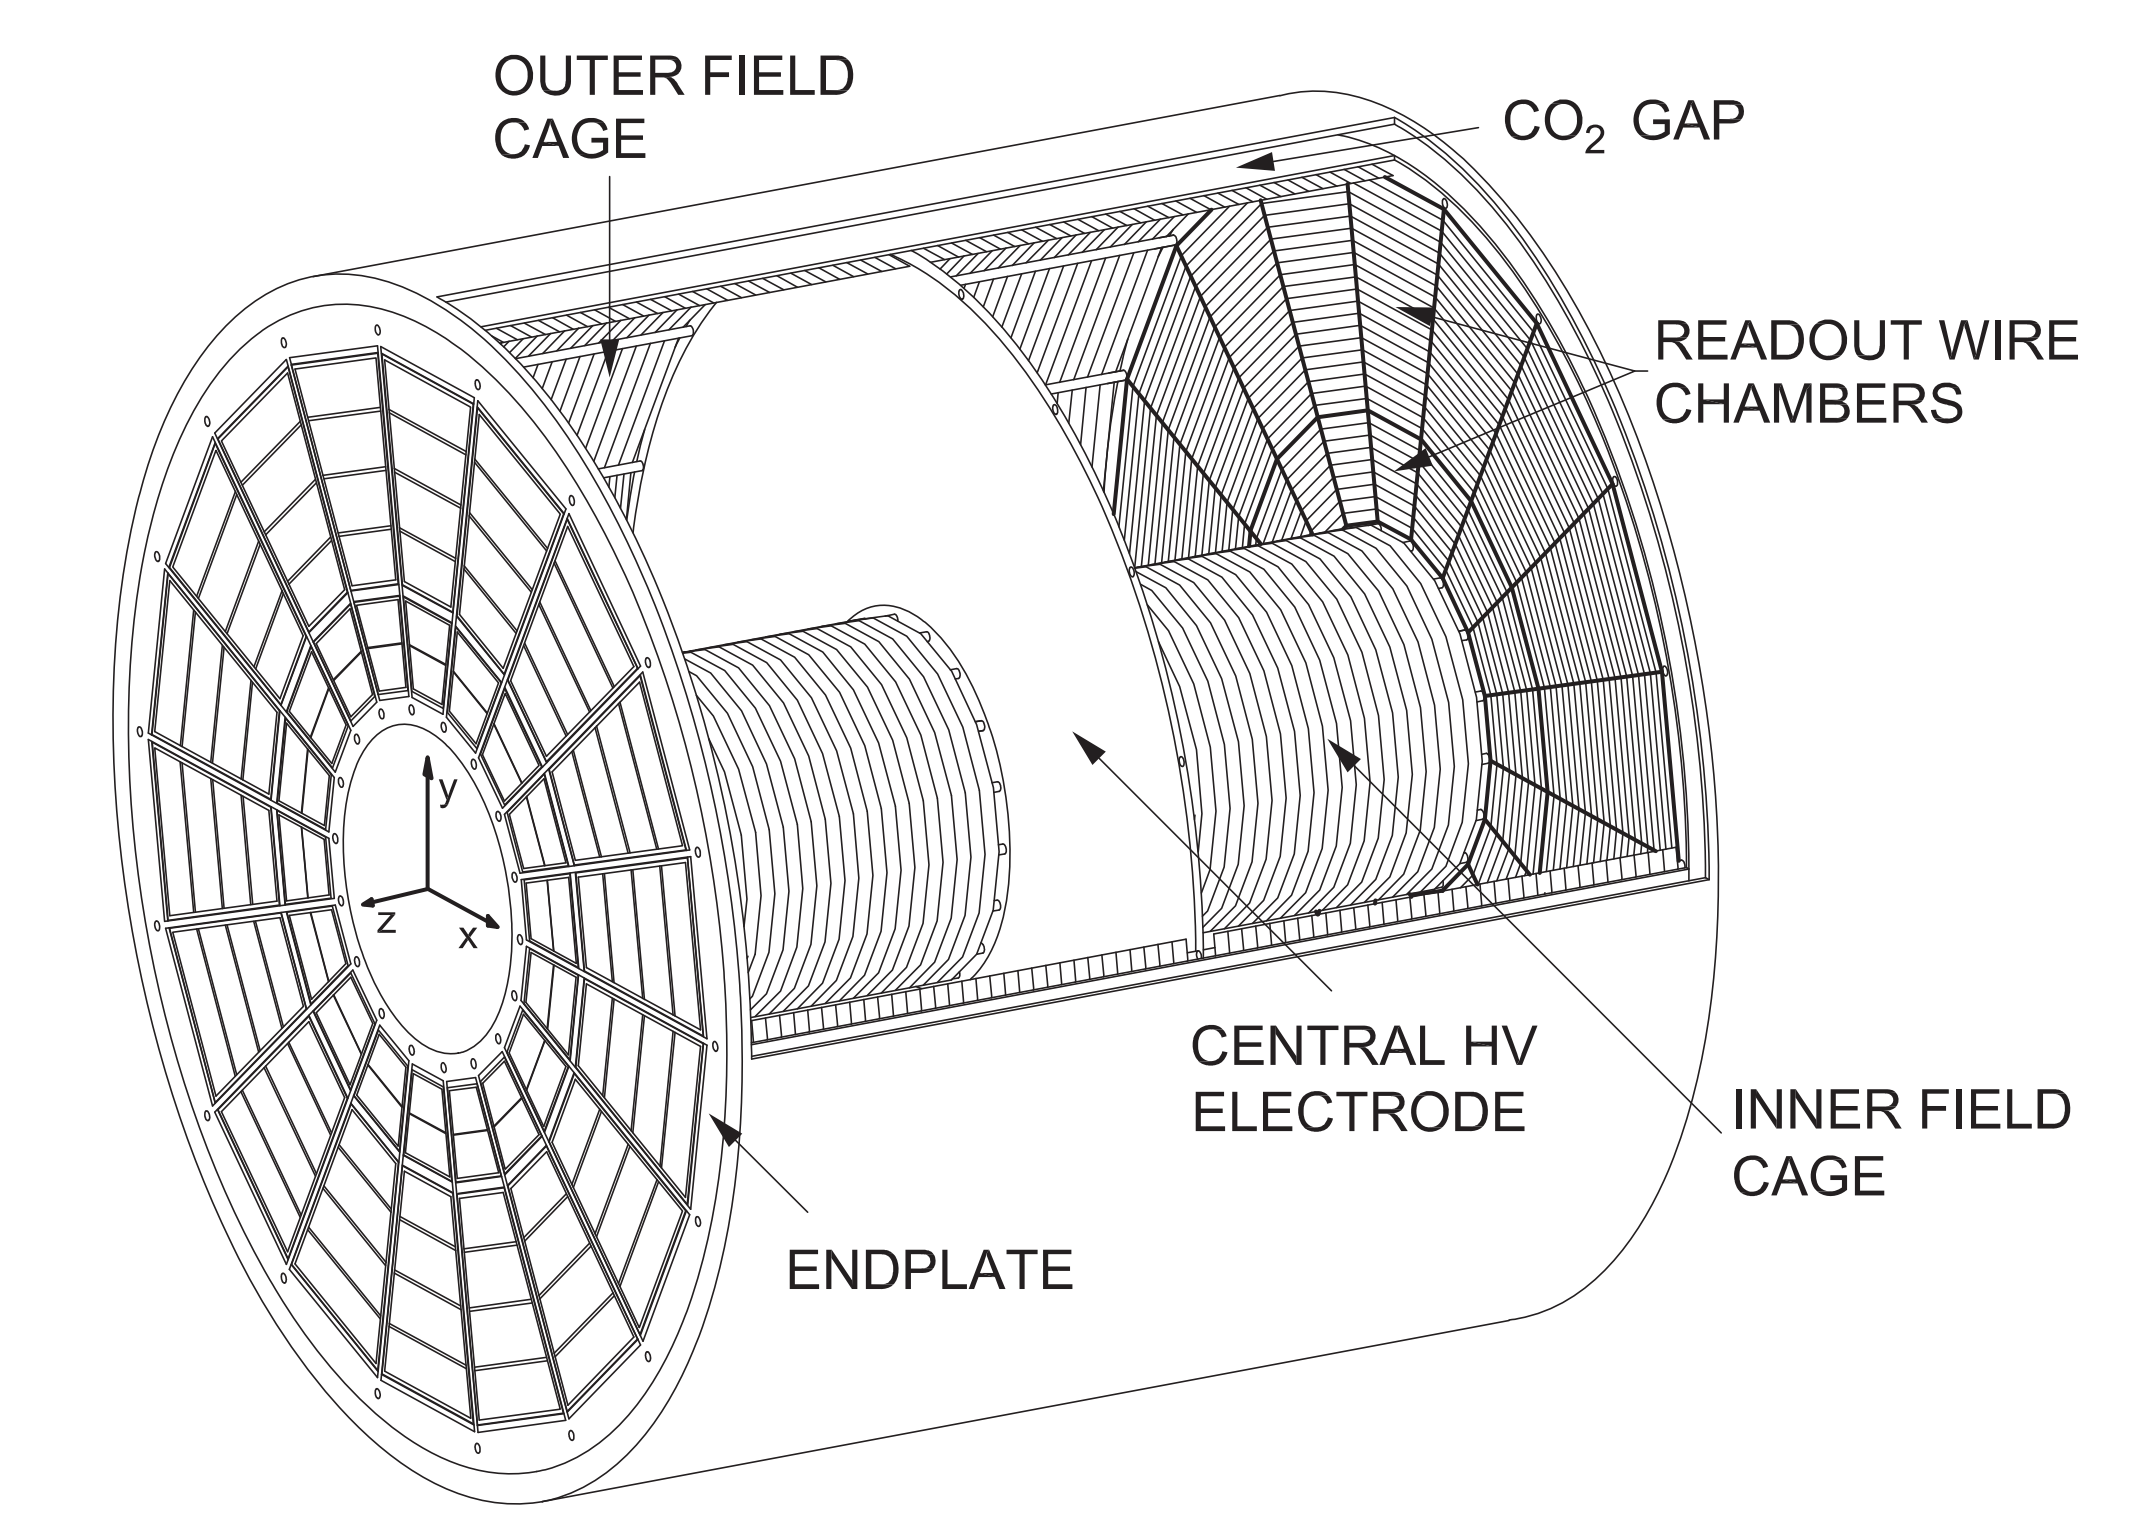
\includegraphics[width=0.9\textwidth]{figures/experiment/tpc_schematic.png}
    \caption{A schematic of the TPC field cage, taken from~\cite{TPC1}}
    \label{fig:tpc_schematic}
\end{figure}

Readout chambers with design based off of the Multi-Wire Proportional Chamber (MWPC) technique are installed at both endplates. In short, these chambers contain an array of wires held at a high voltage are placed in front of a plane of pads held at ground. The electrons that drift towards the endplate pass through this region, which causes a localized cascade of ionization\footnote{Often called a Townsend avalanche, where the ionizing electrons from the initial ionization of the ionizable gas ionize the ionizable gas, creating more ionizing electrons to ionize more ionizable gas...} that is ultimately collected by the pads. The inner readout chamber has 5504 total pads, while the outer readout chamber (i.e. the one actually visible in Figure~\ref{fig:tpc_schematic}) has nearly 10000. The pads are grouped into 18 trapezoidal sectors, each of which covers 20$^\circ$ in azimuth. Unfortunately the boundaries of these sectors don't contain any pads, resulting in very narrow ``dead zones'' within the azimuthal acceptance of the TPC. Using information from both the ITS and TPC, it is possible to reconstruct particle tracks with a resolution of 1 mm in the transverse plane and 2 mm in the longitudinal direction. The momentum resolution in the transverse plane is also very good, staying below 5\% from zero to well over 100 GeV/c.

The TPC is also capable of providing information that can be used to identify particles. As a charged particle travels through the active volume of the TPC, it loses energy as it ionizes the gas in a way that only depends on the particle's velocity. This energy loss is often described by the Bethe-Bloch formula~\cite{BetheBlochPDG}
\begin{equation}
    \left\langle-\frac{d E}{d x}\right\rangle=K z^2 \frac{Z}{A} \frac{1}{\beta^2}\left[\ln \frac{2 m_e c^2 \beta^2 \gamma^2}{I}-\beta^2-\frac{\delta(\beta \gamma)}{2}\right]
\end{equation}
where $K$ is a constant coefficient ($\approx 0.31$ MeV mol$^{-1}$ cm$^2$), $z$ is the charge of the particle, $Z$ and $A$ are the atomic and mass numbers of the gas, $\beta$ is the velocity of the particle in units of the speed of light, $\gamma$ is the Lorentz factor, $m_e$ is the mass of the electron, $c$ is the speed of light, and $I$ is the mean excitation energy of the gas. An important feature of this equation is that most of the parameters depend on the gas mixture and the mass of the electron. For a fixed gas mixture, this equation gives a relationship between the energy (loss) and the velocity of the particle. As the momentum of the particle is known, the mass (and therefore the particle species) can be determined. To see this explicitly, it is useful to look at a common parameterization of the Bethe-Bloch formula~\cite{BetheBlochALEPH},
\begin{equation}
    f(\beta \gamma)=\frac{P_1}{\beta^{P_4}}\left(P_2-\beta^{P_4}-\ln \left(P_3+\frac{1}{(\beta \gamma)^{P_5}}\right)\right),
\end{equation}
where parameters $P_i$ only depend on the gas mixture. Rewriting this equation in terms of the momentum $p$ of the particle gives a curve for each particle species with mass $m_i$,
\begin{equation}
    \label{eq:bethe_bloch_par}
    f(p, m_i)= P_1 \left(\frac{\sqrt{m_i^2 + p^2}}{p}\right)^{P_4} \left(P_2 - \left(\frac{p}{\sqrt{m_i^2 + p^2}}\right)^{P_4}  - \ln \left(P_3 + \frac{m_i^{P_5}}{p^{P_5}} \right) \right).
\end{equation}

\begin{figure}
    \centering
    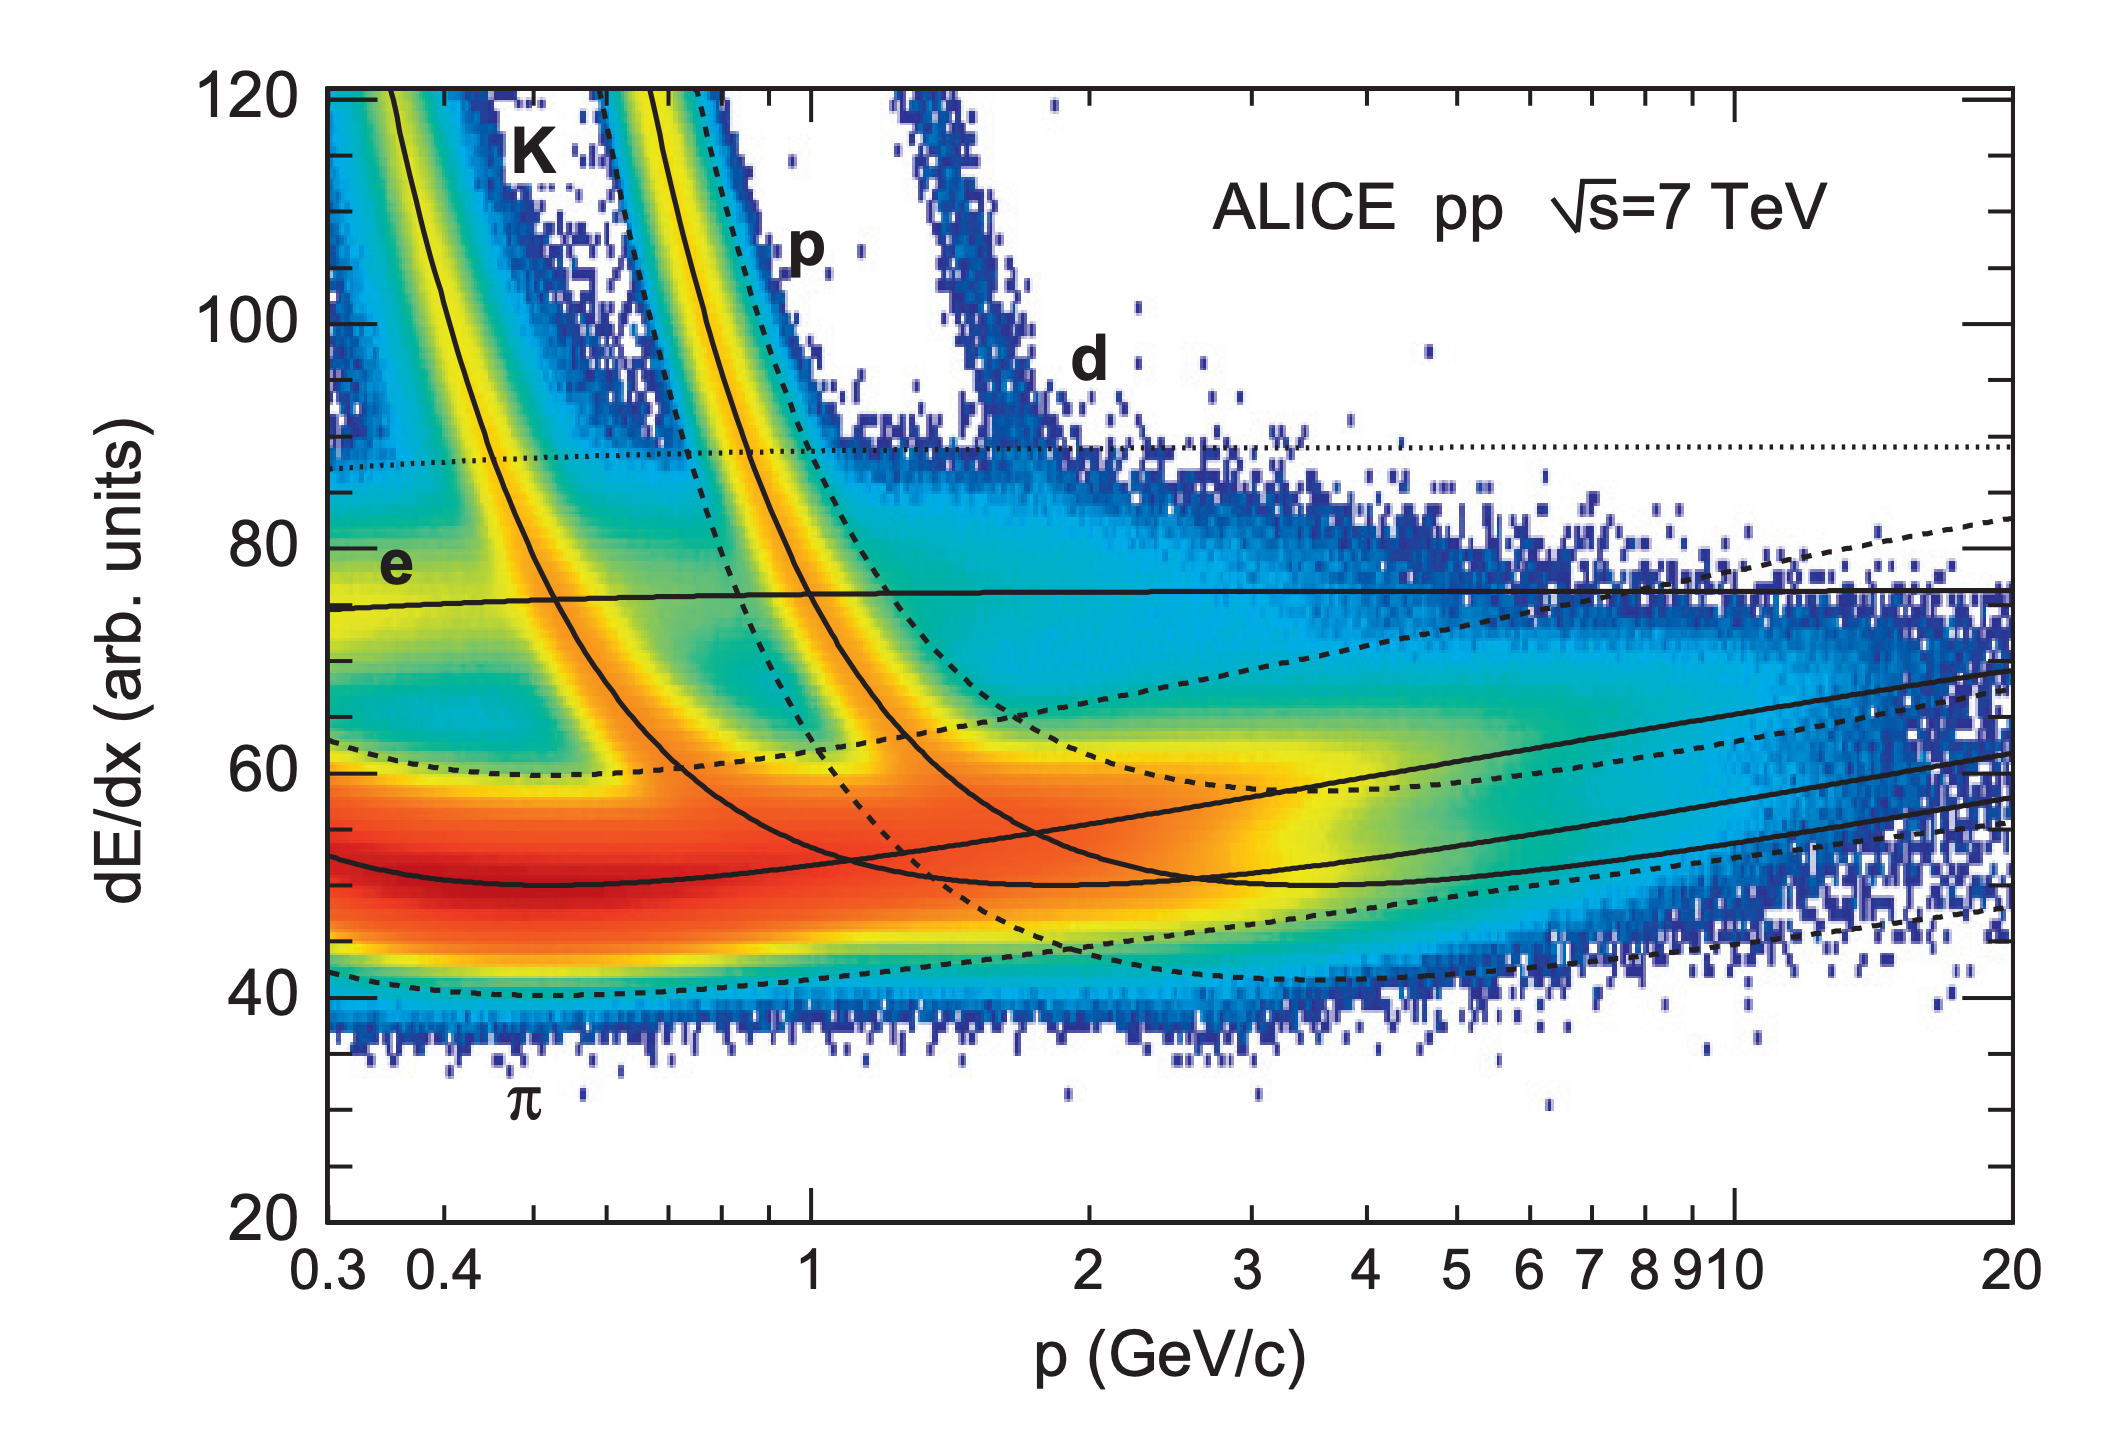
\includegraphics[width=0.9\textwidth]{figures/experiment/tpc_pid_curves.png}
    \caption{The energy loss signal for different particle species using the ALICE TPC gas mixture, taken from~\cite{BetheBlochALEPH}. The solid lines represent the expected energy loss signal for each particle species (Equation~\ref{eq:bethe_bloch_par}).}
    \label{fig:tpc_pid_curves}
\end{figure}

Examples of the energy loss signal for different particle species using the ALICE TPC gas mixture can be seen in Figure~\ref{fig:tpc_pid_curves}. Note that while there are clearly defined lines for each particle species from Equation~\ref{eq:bethe_bloch_par}, the actual signal is spread out around these lines due to the energy loss and momentum resolution of the TPC. Furthermore, many of the curves intersect at higher momentum. As such, it is useful to define the quantity 
\begin{equation}
n\sigma_{\text{TPC}} = \frac{\langle dE/dx \rangle_{\text{meas}} - \langle dE/dx \rangle_{\text{exp}}}{\sigma_{\text{TPC}}},
\end{equation}
which is the number of standard deviations away from the expected energy loss signal for a given particle species. If an unidentified particle has an $n\sigma_{\text{TPC}}$ value close to zero, it is likely that the particle is of that species. However, when investigating a specific particle species, compromises must be made--requiring a low $n\sigma_{\text{TPC}}$ value may result in less contamination from other particle species, but also yields lower statistics.

\section{The Time of Flight detector}
\label{sec:tof}

The Time of Flight (TOF) detector~\cite{TOF1} is a large array of Multi-gap Resistive Plate Chambers (MRPCs)~\cite{TOF2} that is used to measure the time of flight of charged particles from the nominal interaction point. The TOF is located directly outside of the TPC at a radius of around 3.7 meters, and covers the pseudorapidity range $|\eta| < 0.9$. It consists of 1593 MRPC strips, arranged in 18 sectors along the azimuthal direction. Each MRPC strip has two rows of 48 pickup pads with area 3.5 $\times$ 2.5 cm$^2$, to ensure low occupancy even in the most crowded events. This gives a total of 96 pads per strip and 152928 readout channels in total. The TOF MRPC has a double-stack structure; each of the two stacks has five gas gaps each. The resistive plates are made of standard soda-lime glass sheets. The gap (250 µm) is created by commercial fishing line stretched over the glass sheets. The average MRPC time resolution, including the effects of the full front-end and readout electronics, was measured to be better than 50 ps in a beam test setup.

\begin{figure}
    \centering
    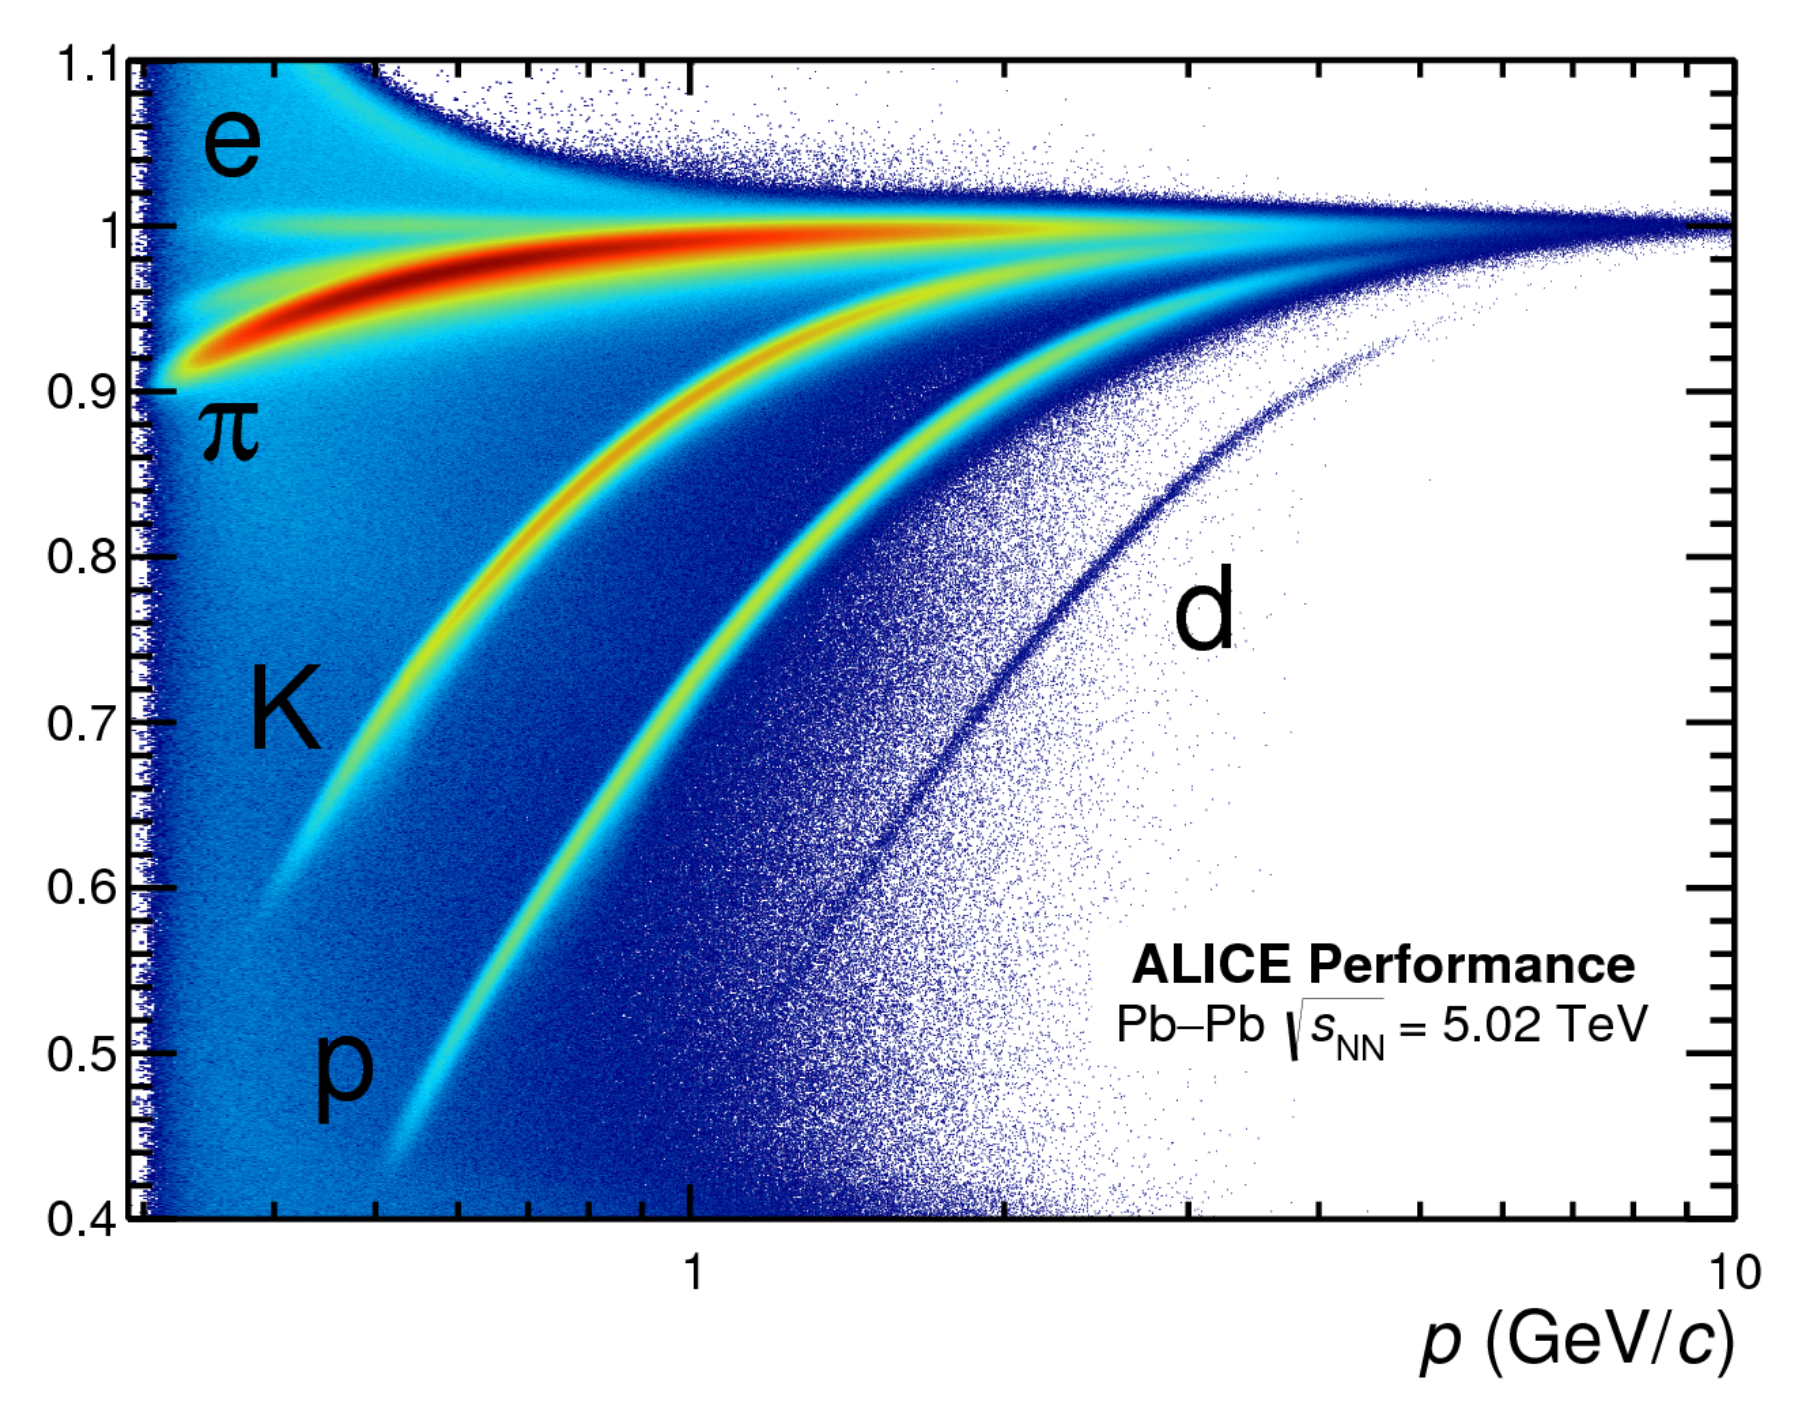
\includegraphics[width=0.9\textwidth]{figures/experiment/tof_pid_curves.png}
    \caption{The time of flight signal $\beta_{\text{TOF}}$ measured in 5.02 TeV Pb--Pb collisions for different particle species as a function of momentum~\cite{TOFPIDPlot}. The curves are labeled with the particle species they correspond to.}
    \label{fig:tof_pid_curves}
\end{figure}

The primary goal of the TOF detector is particle identification: the time of flight of a particle is directly related to its velocity (as the TOF is a fixed length away from the interaction point), which can be used with the particle's momentum to determine its mass. More explicitly, the velocity $\beta$ of a particle is given by (in natural units)
\begin{equation}
    \beta_{\text{TOF}} = \frac{L}{t_{\text{TOF}}},
\end{equation}
where $L$ is the distance from the interaction point to the TOF (3.7 meters) and $t_{\text{TOF}}$ is the time of flight of the particle. Using $p =  m \frac{\beta}{\sqrt{1-\beta^2}}$, $\beta_{\text{TOF}}$ can be written as a function of $p$ for a particle of mass $m_i$,
\begin{equation}
    \beta_{\text{TOF}}(p, m_i) = \frac{p}{\sqrt{p^2 + m_i^2}}.
\end{equation}
Much like the TPC, plotting the TOF signal versus momentum provides a unique curve for each particle species, as shown in Figure~\ref{fig:tof_pid_curves}. Also much like the TPC, the signal is spread out around the expected curve due to the timing resolution of the TOF and momentum resolution of the TPC $+$ ITS. As such, the quantity
\begin{equation}
n\sigma_{\text{TOF}} = \frac{\beta_{\text{meas}} - \beta_{\text{exp}}}{\sigma_{\text{TOF}}},
\end{equation}
is defined, which serves a similar purpose to $n\sigma_{\text{TPC}}$.



\section{The Electromagnetic Calorimeter}

The Electromagnetic Calorimeter (EMCal)~\cite{EMCAL1, EMCAL2} is a sampling calorimeter that consists of lead and polystyrene scintillator layers. The EMCal is made of towers, which are stacks of 76 lead layers (1.44 mm thick) and 77 polystyrene layers (1.76 mm thick). Each tower has a size of about 6.0 $\times$ 6.0 $\times$ 24.6 cm$^3$ and has an individual readout. The towers are arranged into 2 $\times$ 2 groups called modules, which are the smallest units of the detector. The modules are further assembled into larger supermodules (12 $\times$ 24 modules), each weighing about 7.7 metric tons. The EMCal has a total of 10 full-size supermodules and 2 one-third size supermodules, corresponding to 3072 modules and 12,288 towers. It covers a pseudorapidity range of $|\eta| < 0.7$ and an azimuthal angle range of  $\Delta\varphi = 107^\circ$. It is positioned around 4.5 meters from the beam line, between the space-frame support structure and the L3 magnet coils. Schematics of the detector components can be seen in Figure~\ref{fig:emcal_schematic}. While not used in this thesis, the University of Texas at Austin was involved in the commissioning of the EMCal, and thus it is worth mentioning for historical purposes.

\begin{figure}
    \centering
    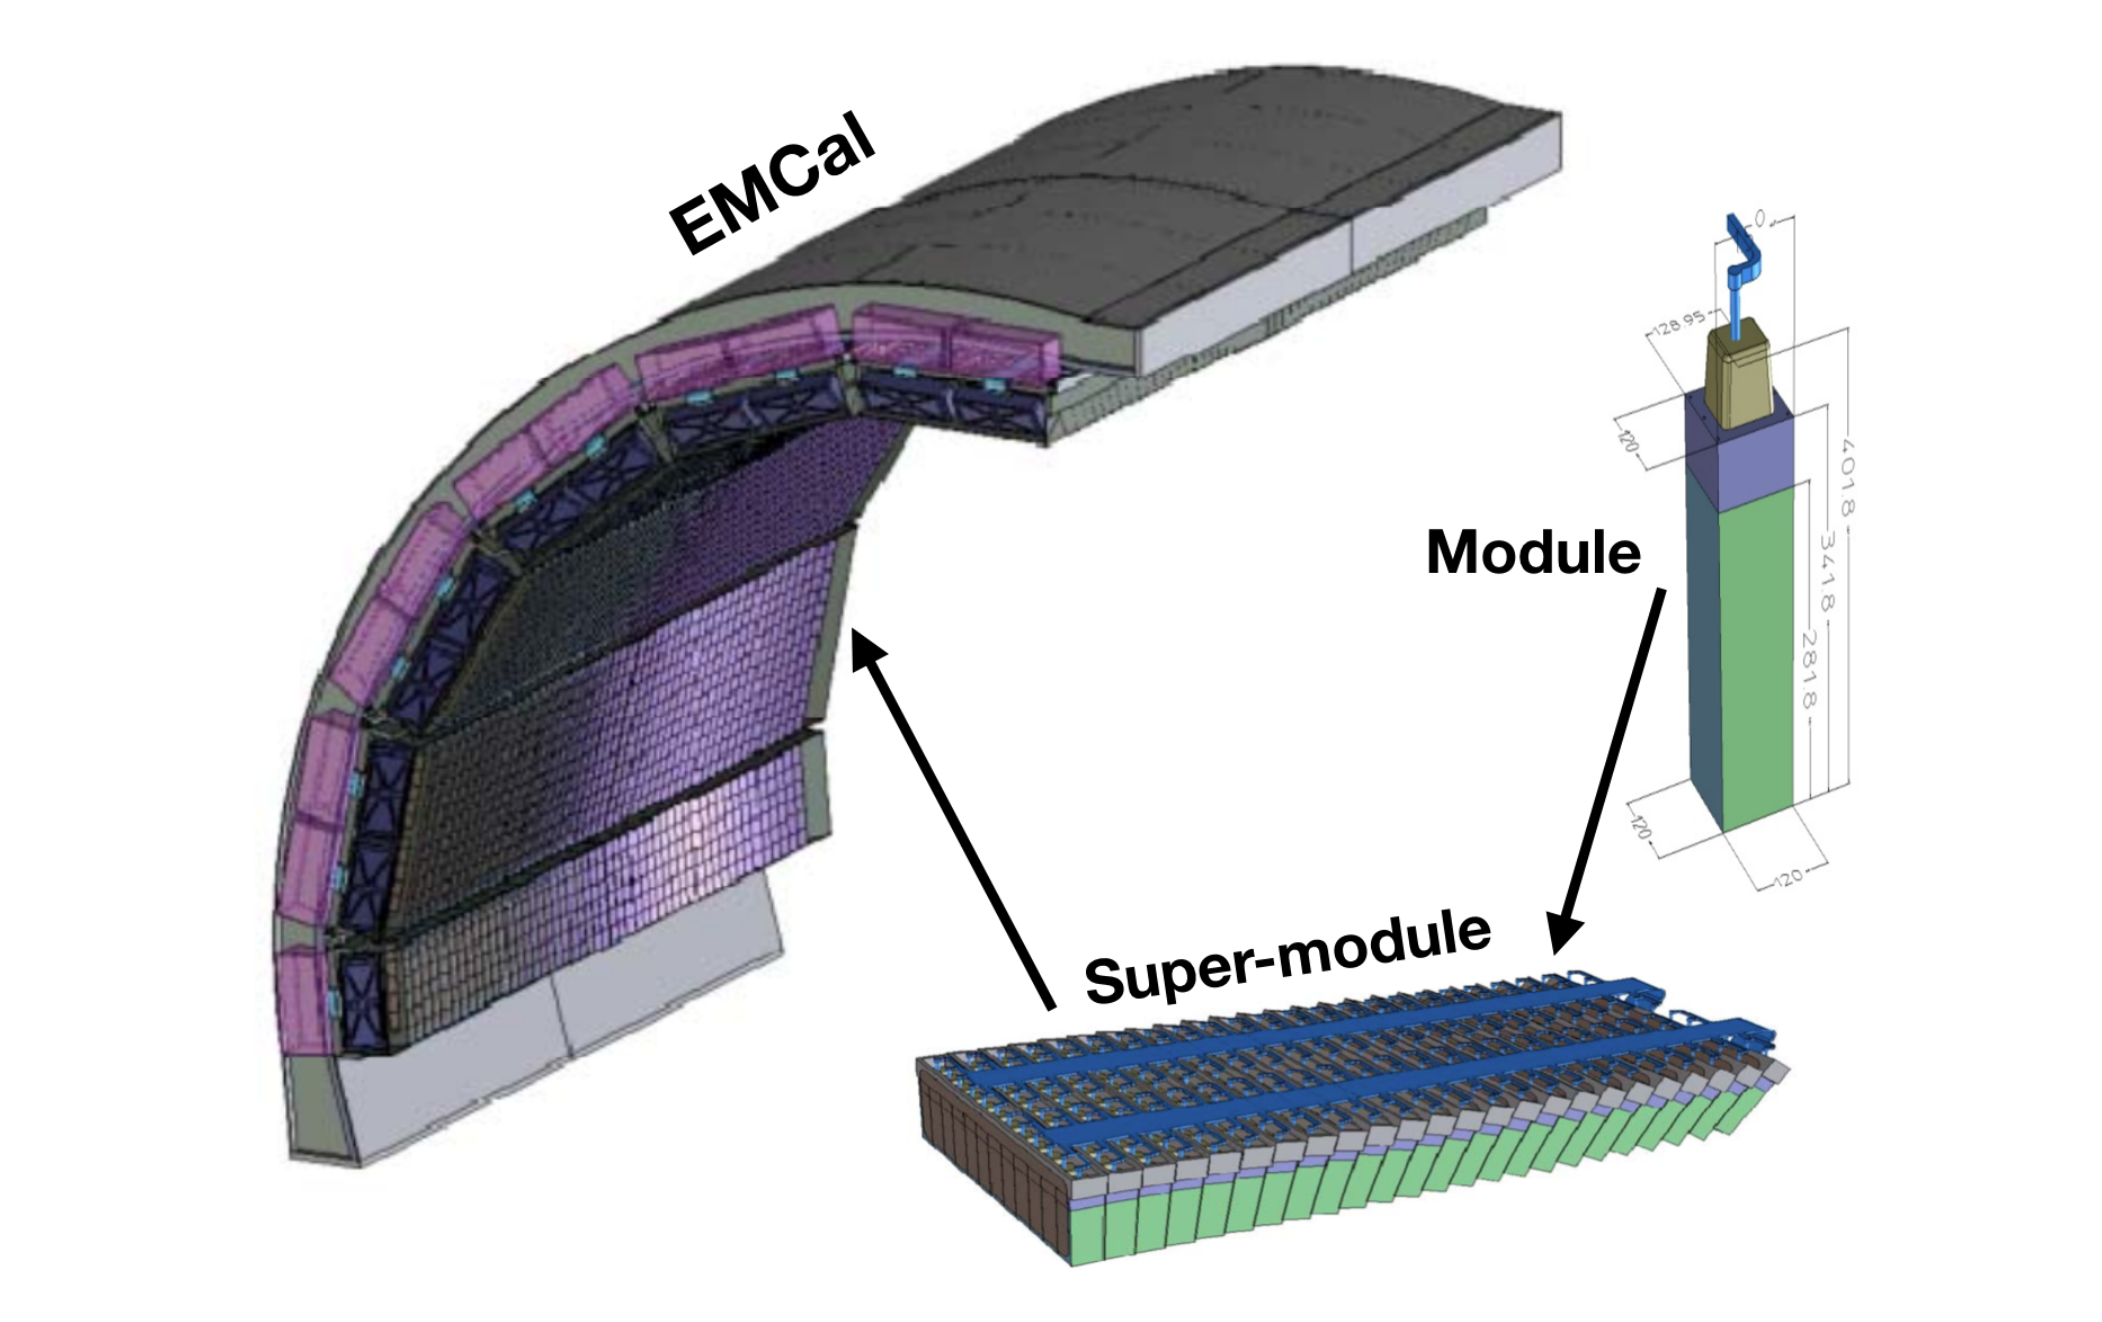
\includegraphics[width=0.9\textwidth]{figures/experiment/emcal_schematic.png}
    \caption{A schematic of the EMCal~\cite{ERIN123}, along with the module and supermodule structure~\cite{ERIN124}.}
    \label{fig:emcal_schematic}
\end{figure}

\section{The VZERO Detector}

The VZERO detector~\cite{VZERO} consists of two end-cap scintillators: the V0A, located in the forward pseudorapidity region ($2.8 < \eta < 5.1$); and the V0C, located in the backward region ($-3.7 < \eta < -1.7$). While most of the interesting physics lies at midrapidity, these detectors are vital for estimating the collision centrality (as discussed in Section~\ref{sec:collision_centrality}). The VZERO detectors also provide a trigger for the other detectors: whenever a coincident signal occurs in the V0A and V0C, a collision event must have occured between the two detectors. The VZERO system is also used to monitor LHC beam conditions and reject beam-gas and beam-halo events. As the data analyzed in this thesis is from p--Pb collisions, only information from the V0A detector--which faces the lead ion beam--is used for determining the multiplicity percentile of the collision events.
% \chapter{$\Lambda$ Production In and Out-of Jets: Analysis Overview}
This chapter will provide a high-level description of the main analysis topic of this dissertation: using the $\Lambda$ baryon to investigate the origins of strangeness enhancement in p-Pb collisions. First, the goal of this analysis will be clearly stated, along with the steps needed to acheive this goal. Then, each step will be described with more detail, including justification. Finally, the analysis will be summarized, and the next chapter will describe the analysis in more detail.

\section{Objective}
While the phrase ``origins of strangeness enhancement'' is concise, it lacks the specificity required to bring the analysis to fruition. In order to make 
\chapter{Analysis Details}
% \chapter{Systematic uncertainties and cross-checks}
\label{chapter_systematics}
Systematic uncertainties are inevitable in any analysis, and the present one is no exception. This chapter describes the various sources of systematic uncertainties that affect the final results, and how their magnitudes are estimated and propagated to the final uncertainties. This chapter also presents the cross-checks that were performed to verify the robustness and consistency of the analysis, and to ensure that no biases were introduced along the way.

\section{Sources of systematic uncertainties}
\label{sec:systematics}

This analysis has three major components:
\begin{enumerate}
\item The generation of the h-$\Lambda$ and h-h $\Delta\varphi$ distributions
\item The extraction of the pairwise yields from the $\Delta\varphi$ distributions
\item The extraction of the near- and away-side widths from the fits of the $\Delta\varphi$ distributions
\end{enumerate}

As such, this section is separated into three subsections, one for each of these components. In each section, the sources of systematic uncertainties are described, and the methods used to estimate their magnitudes are presented.


% \subsection{$\Delta\varphi$ Distribution Generation}
% \label{systematics_dphi}
% As our final yields depend on the $\Delta\varphi$ distributions, we must consider all of the sources of systematic errors that can appear during the generation of these distributions. These sources of systematic errors are as follows.

% \subsubsection{Signal Region Selection}
% While our central points of this analysis involve almost the entirety of our $\Lambda$ signal region, the final result should not depend on which section of the signal region we choose. To investigate this, we vary the signal region in the following ways:

% \begin{itemize}
% \item $1.108 < M_{p\pi} < 1.124$ GeV/$c^2$ (centered, narrow)
% \item $1.112 < M_{p\pi} < 1.120$ GeV/$c^2$ (centered, narrower)
% \item $1.100 < M_{p\pi} < 1.132$ GeV/$c^2$ (centered, wide)
% \item $1.096 < M_{p\pi} < 1.136$ GeV/$c^2$ (centered, wider)
% \end{itemize}

% The resulting $\Delta\varphi$ distributions and ratios to central values for each signal region variation in each multiplicity bin within our central $p_{T, assoc}$ bin are shown in Figures \ref{signal_region_variation_0_20} through \ref{signal_region_variation_50_80}. As we observe no dependence on $\Delta\varphi$, the systematic is calculated as the RMS of the ratios of within the entire $\Delta\varphi$ range for each variation.

% \begin{figure}[ht]
% \centering
% \begin{subfigure}{
% 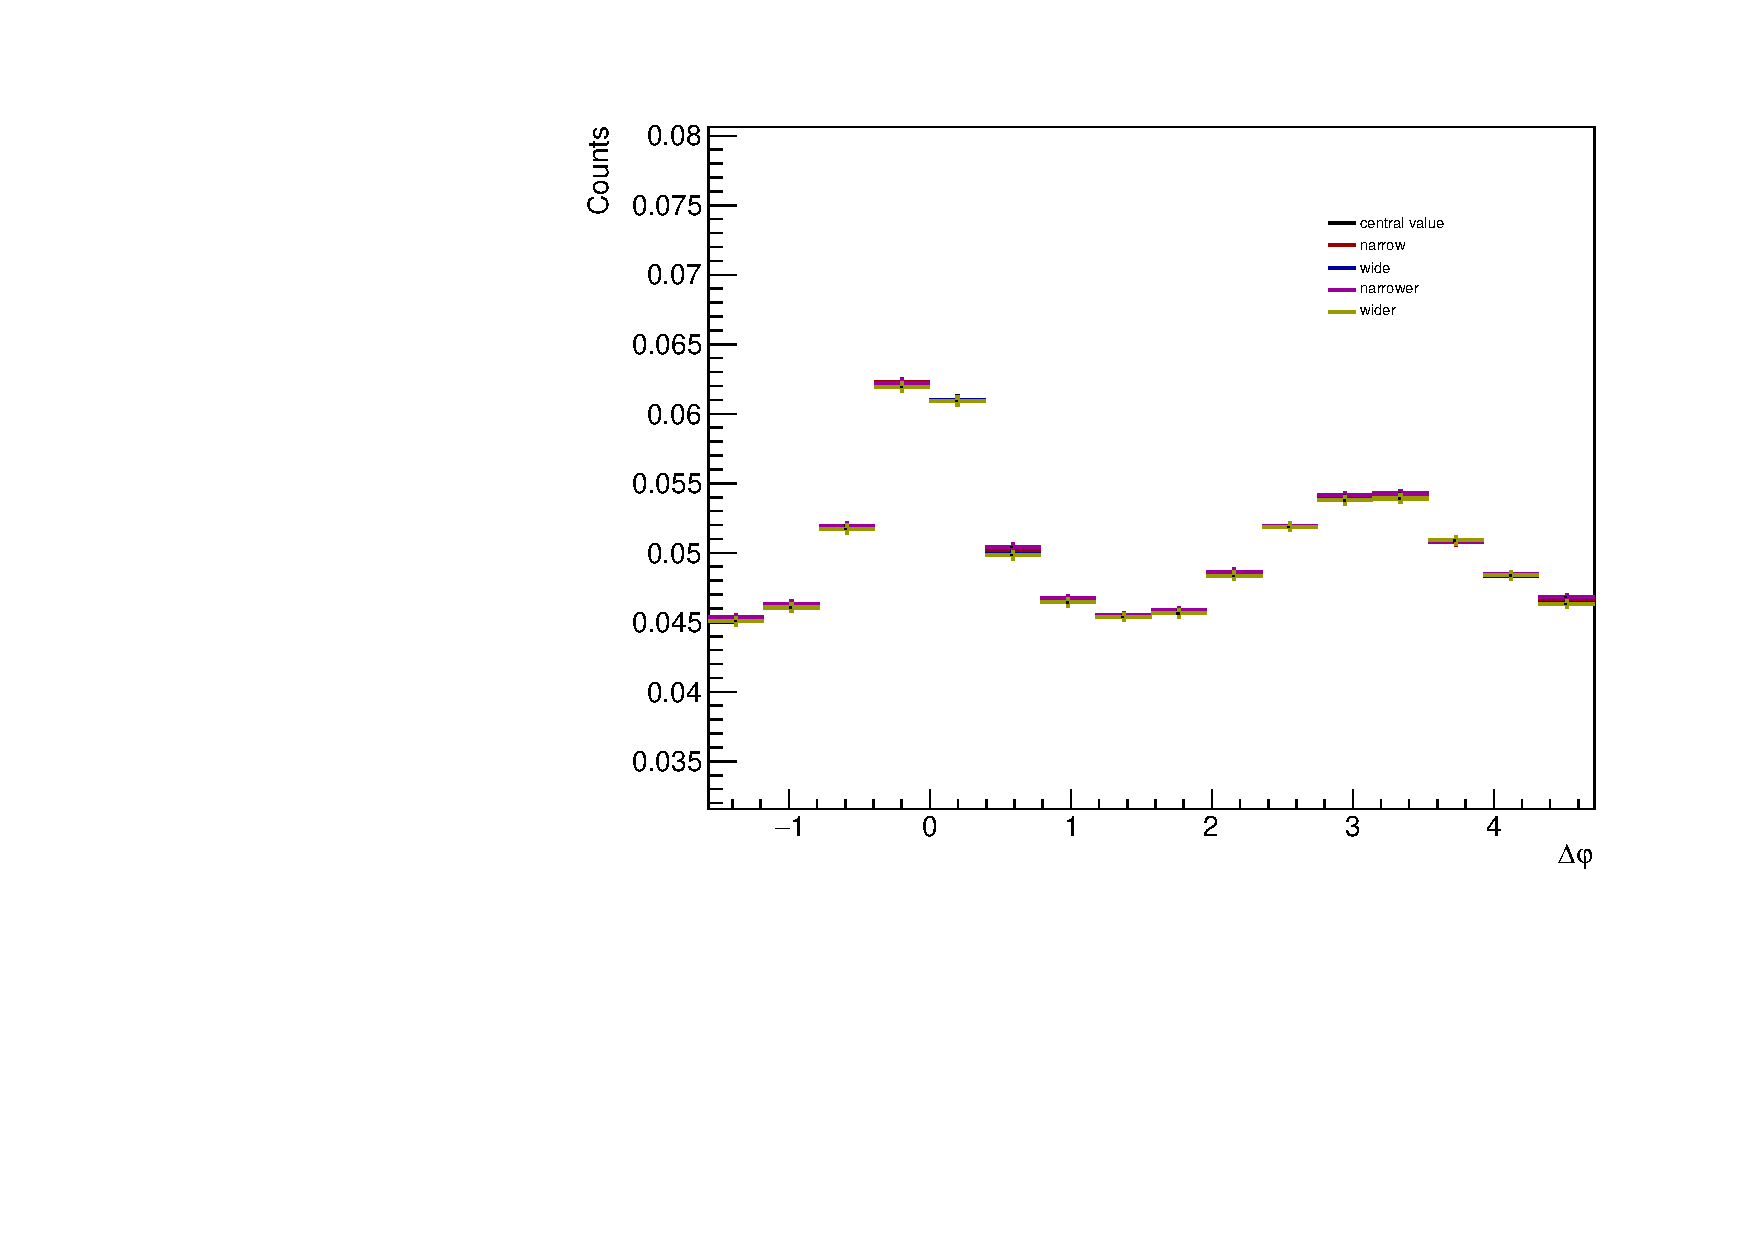
\includegraphics[width=3in]{figures/signal_variations_dphi_0_20.pdf}}
% \end{subfigure}
% \begin{subfigure}{
% 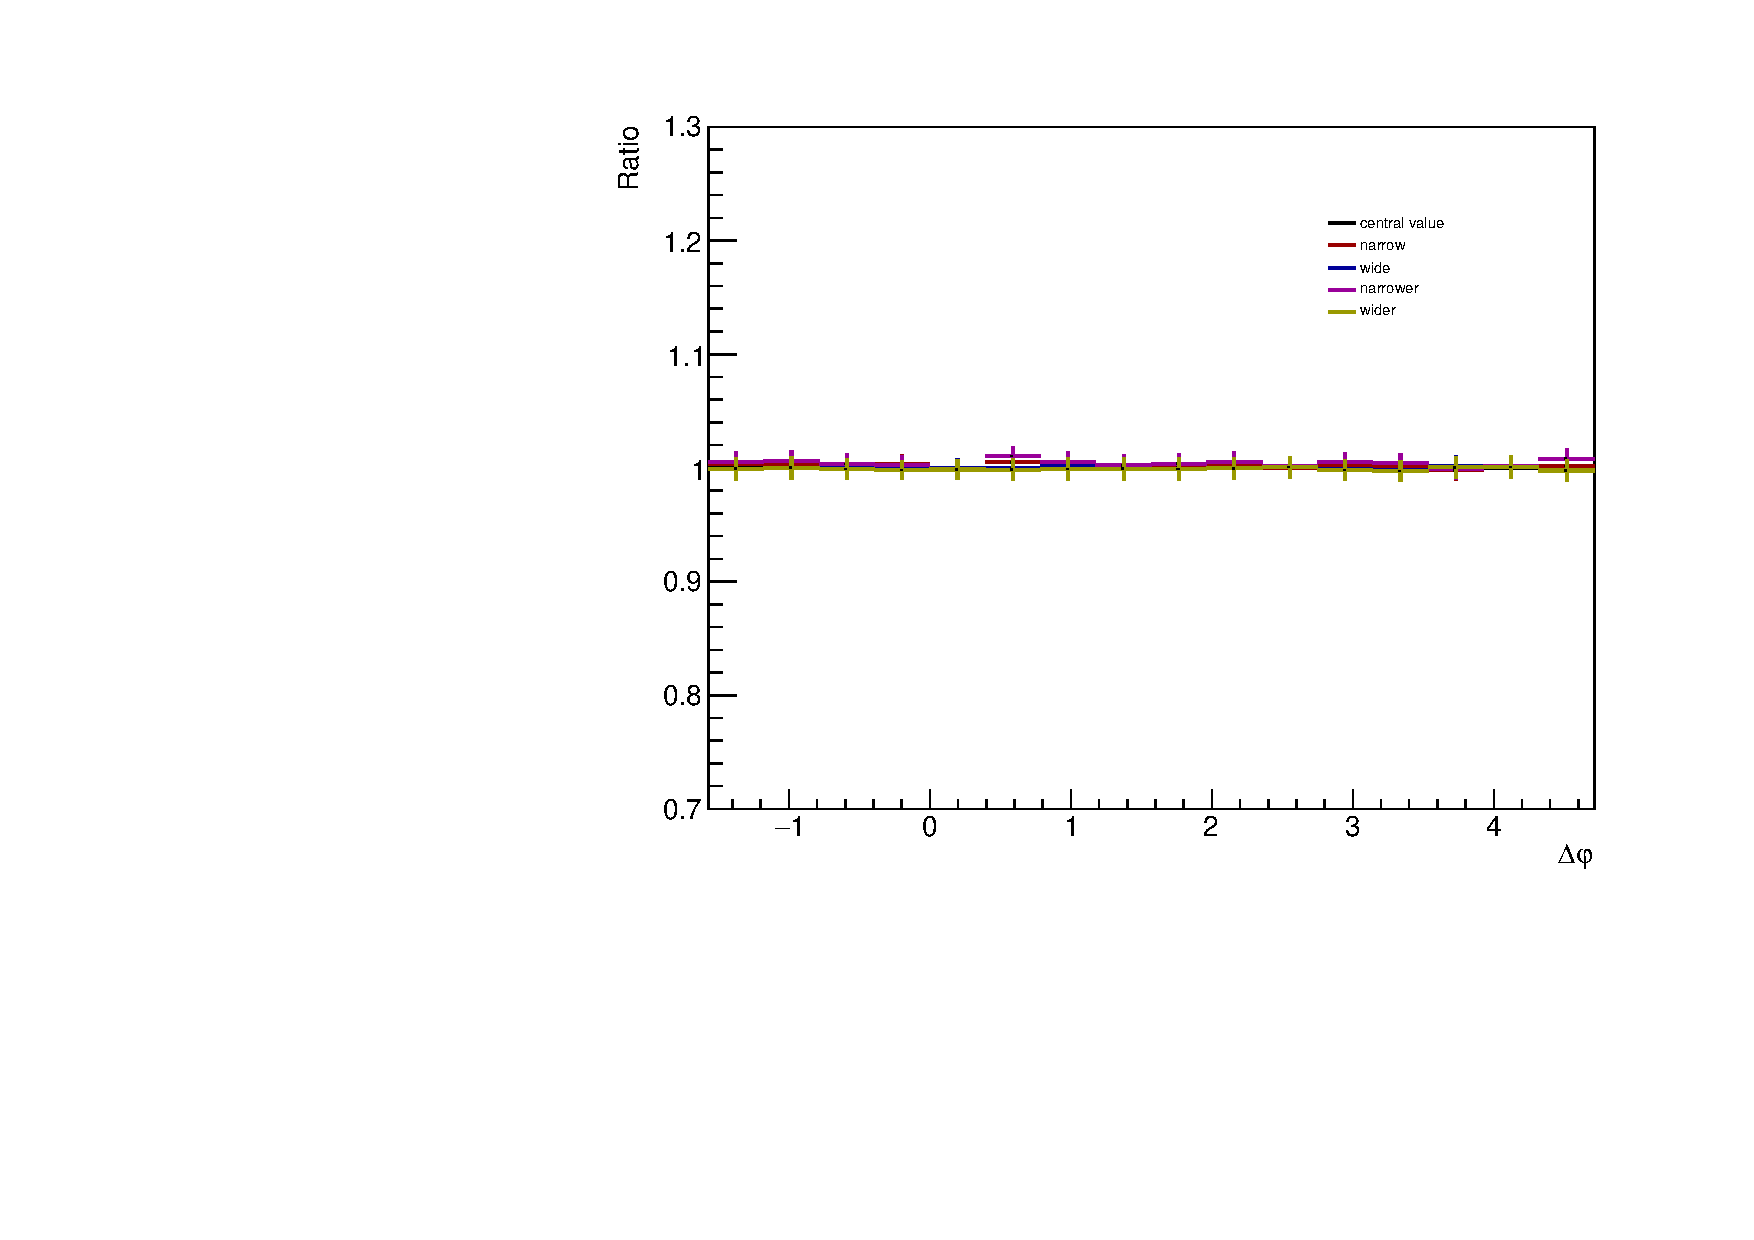
\includegraphics[width=3in]{figures/signal_variations_dphi_0_20_ratio.pdf}}
% \end{subfigure}
% \caption{The $\Delta\varphi$ distributions (left) and corresponding ratios to our central distribution (right) within the 0-20\% multiplicity bin for each of the signal region variations. We observe no dependence on the choice of signal region}
% \label{signal_region_variation_0_20}
% \end{figure}

% \begin{figure}[ht]
% \centering
% \begin{subfigure}{
% 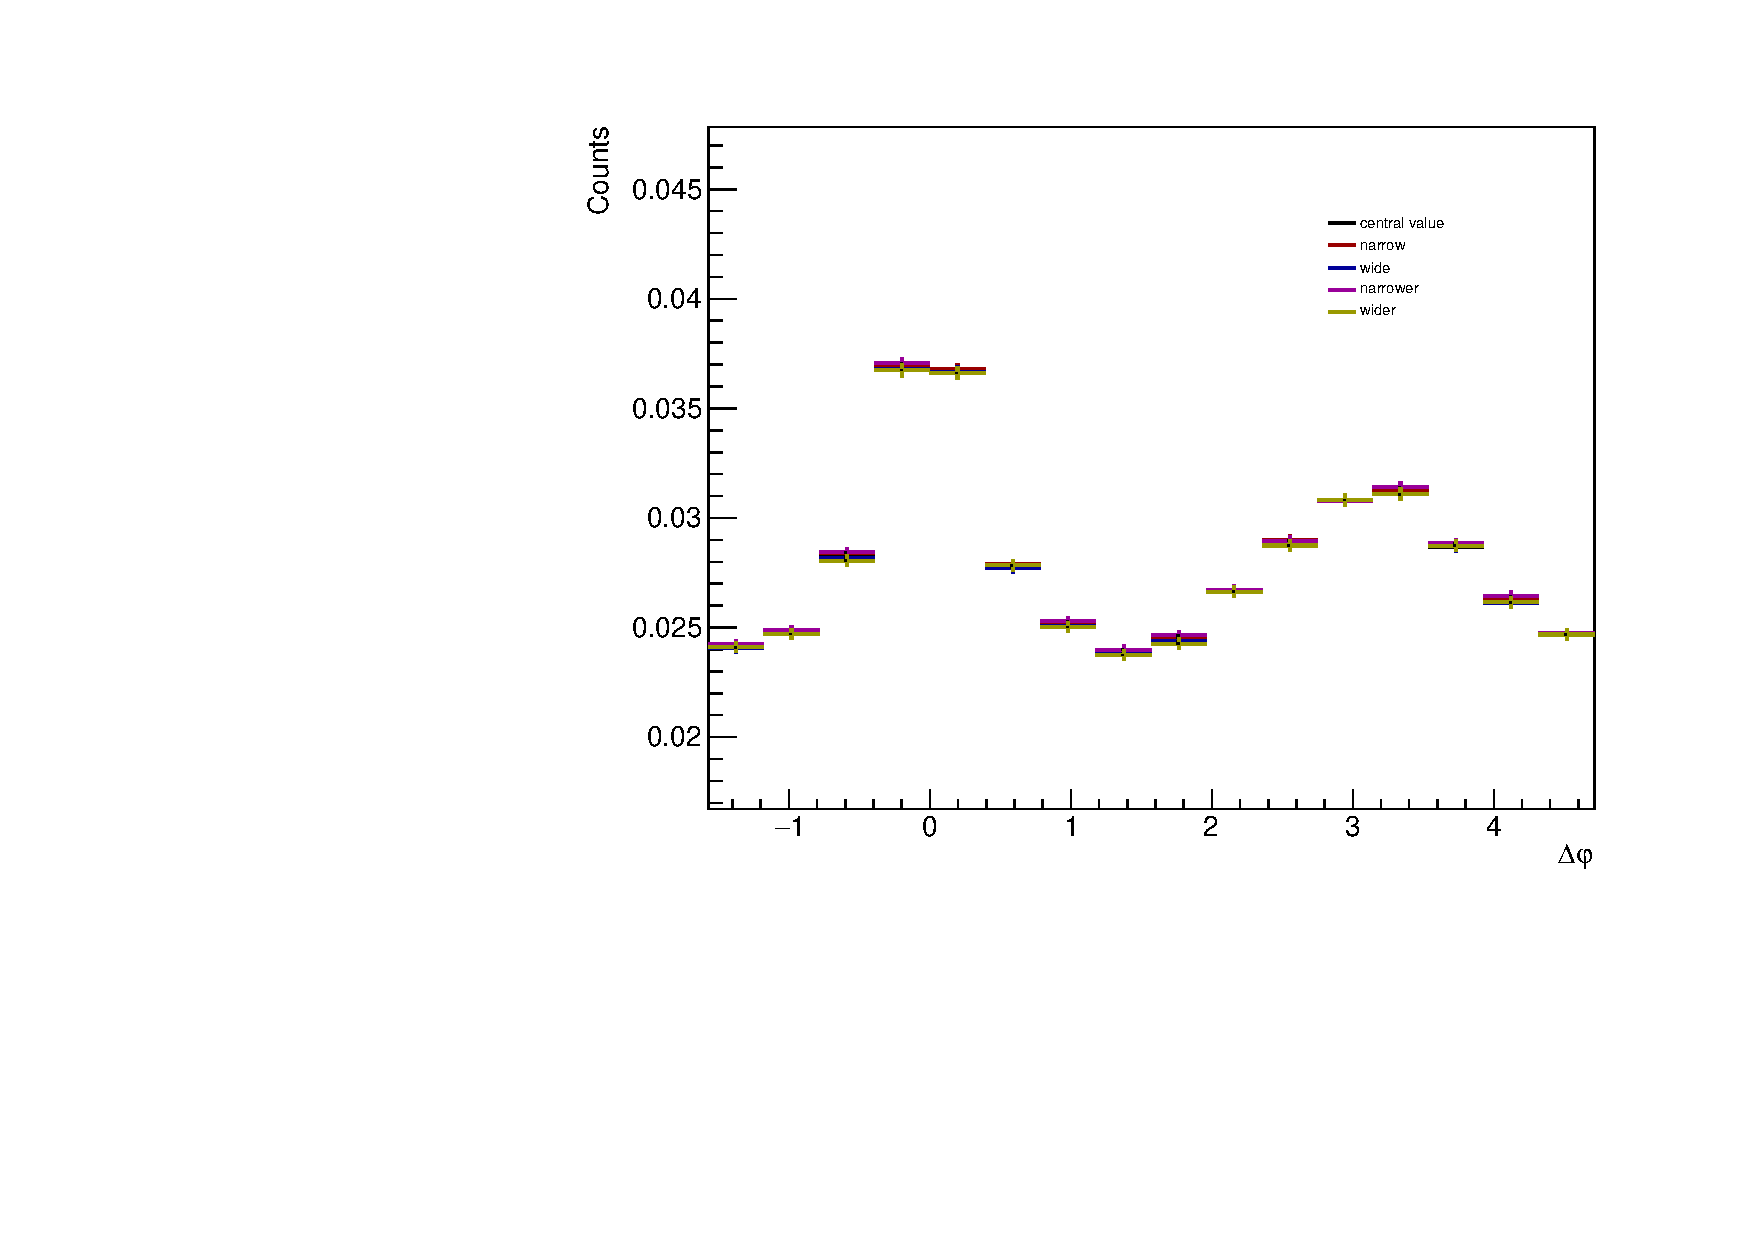
\includegraphics[width=3in]{figures/signal_variations_dphi_20_50.pdf}}
% \end{subfigure}
% \begin{subfigure}{
% 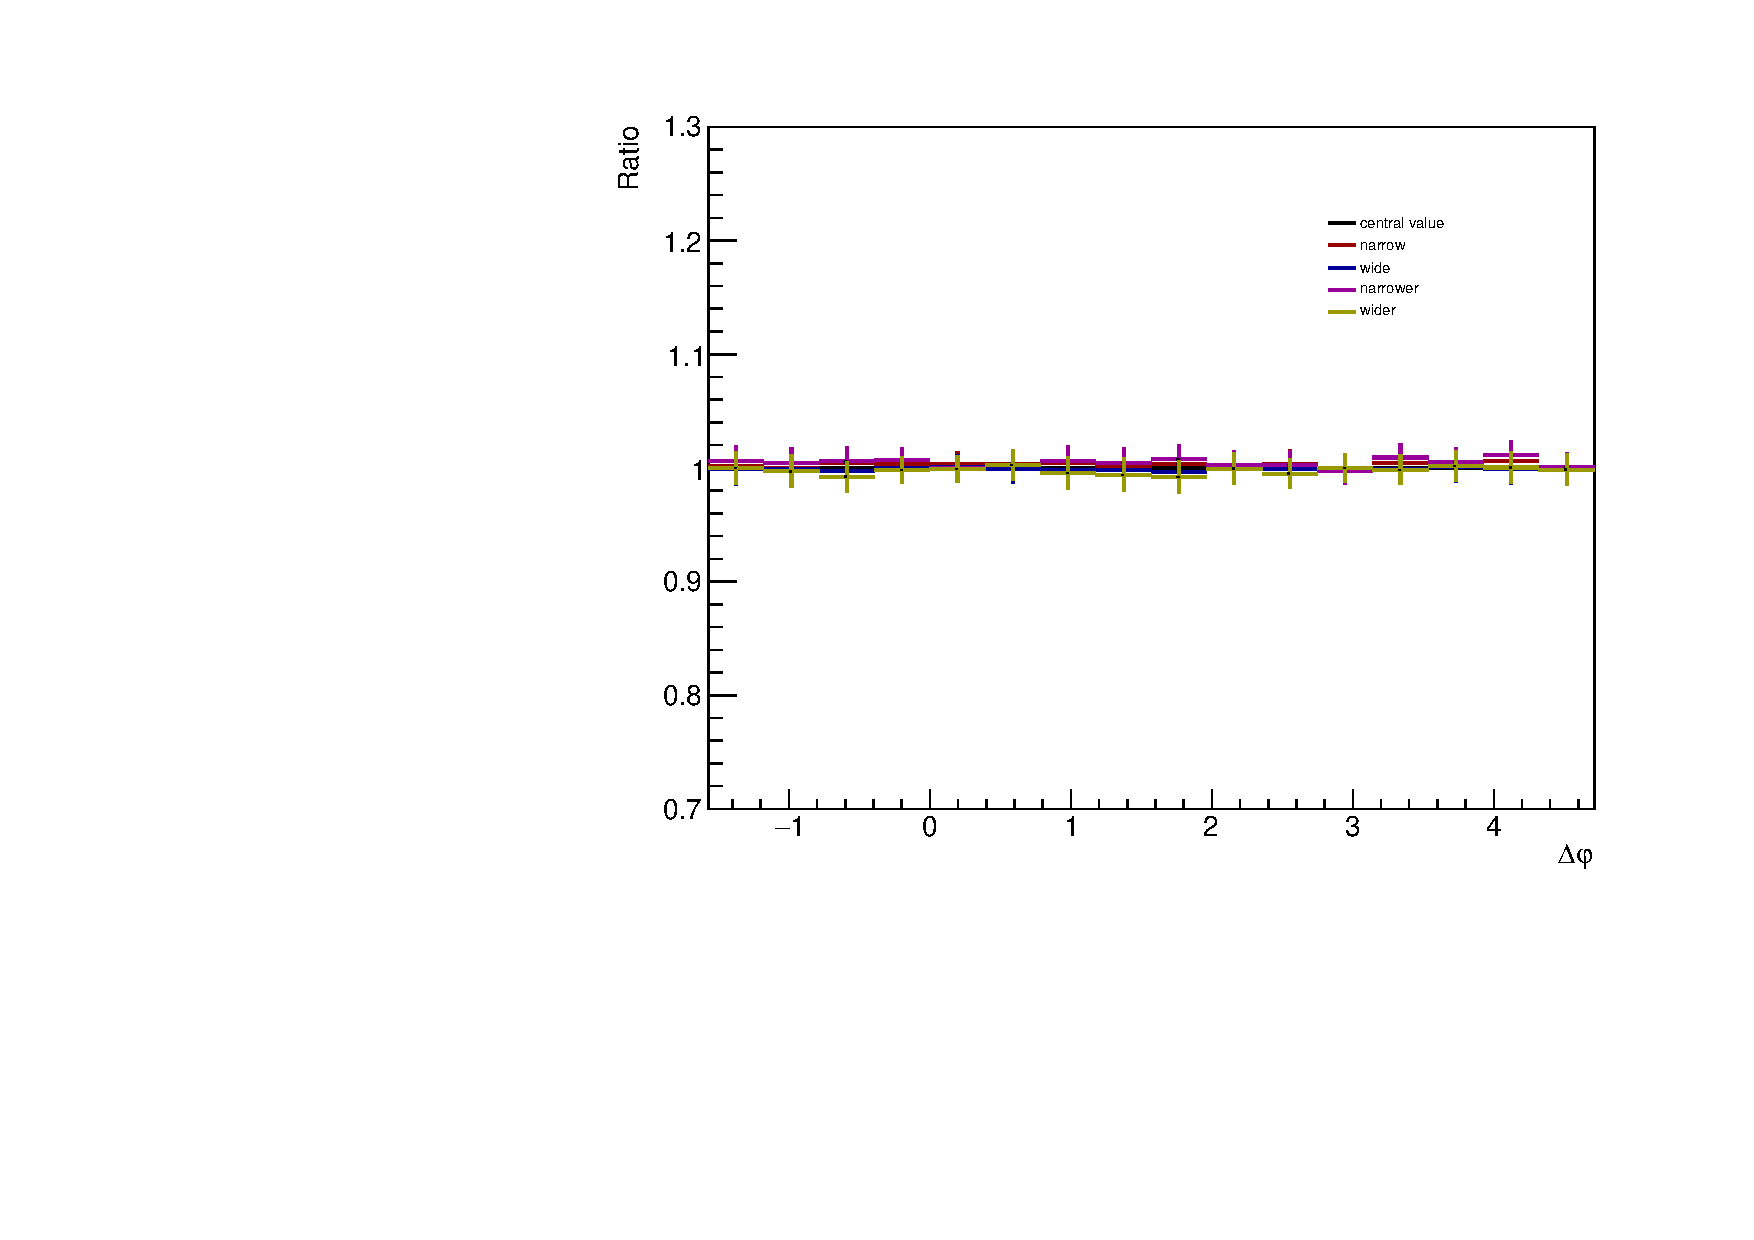
\includegraphics[width=3in]{figures/signal_variations_dphi_20_50_ratio.pdf}}
% \end{subfigure}
% \caption{The $\Delta\varphi$ distributions (left) and corresponding ratios to our central distribution (right) within the 20-50\% multiplicity bin for each of the signal region variations. We observe no dependence on the choice of signal region}
% \label{signal_region_variation_20_50}
% \end{figure}

% \begin{figure}[ht]
% \centering
% \begin{subfigure}{
% 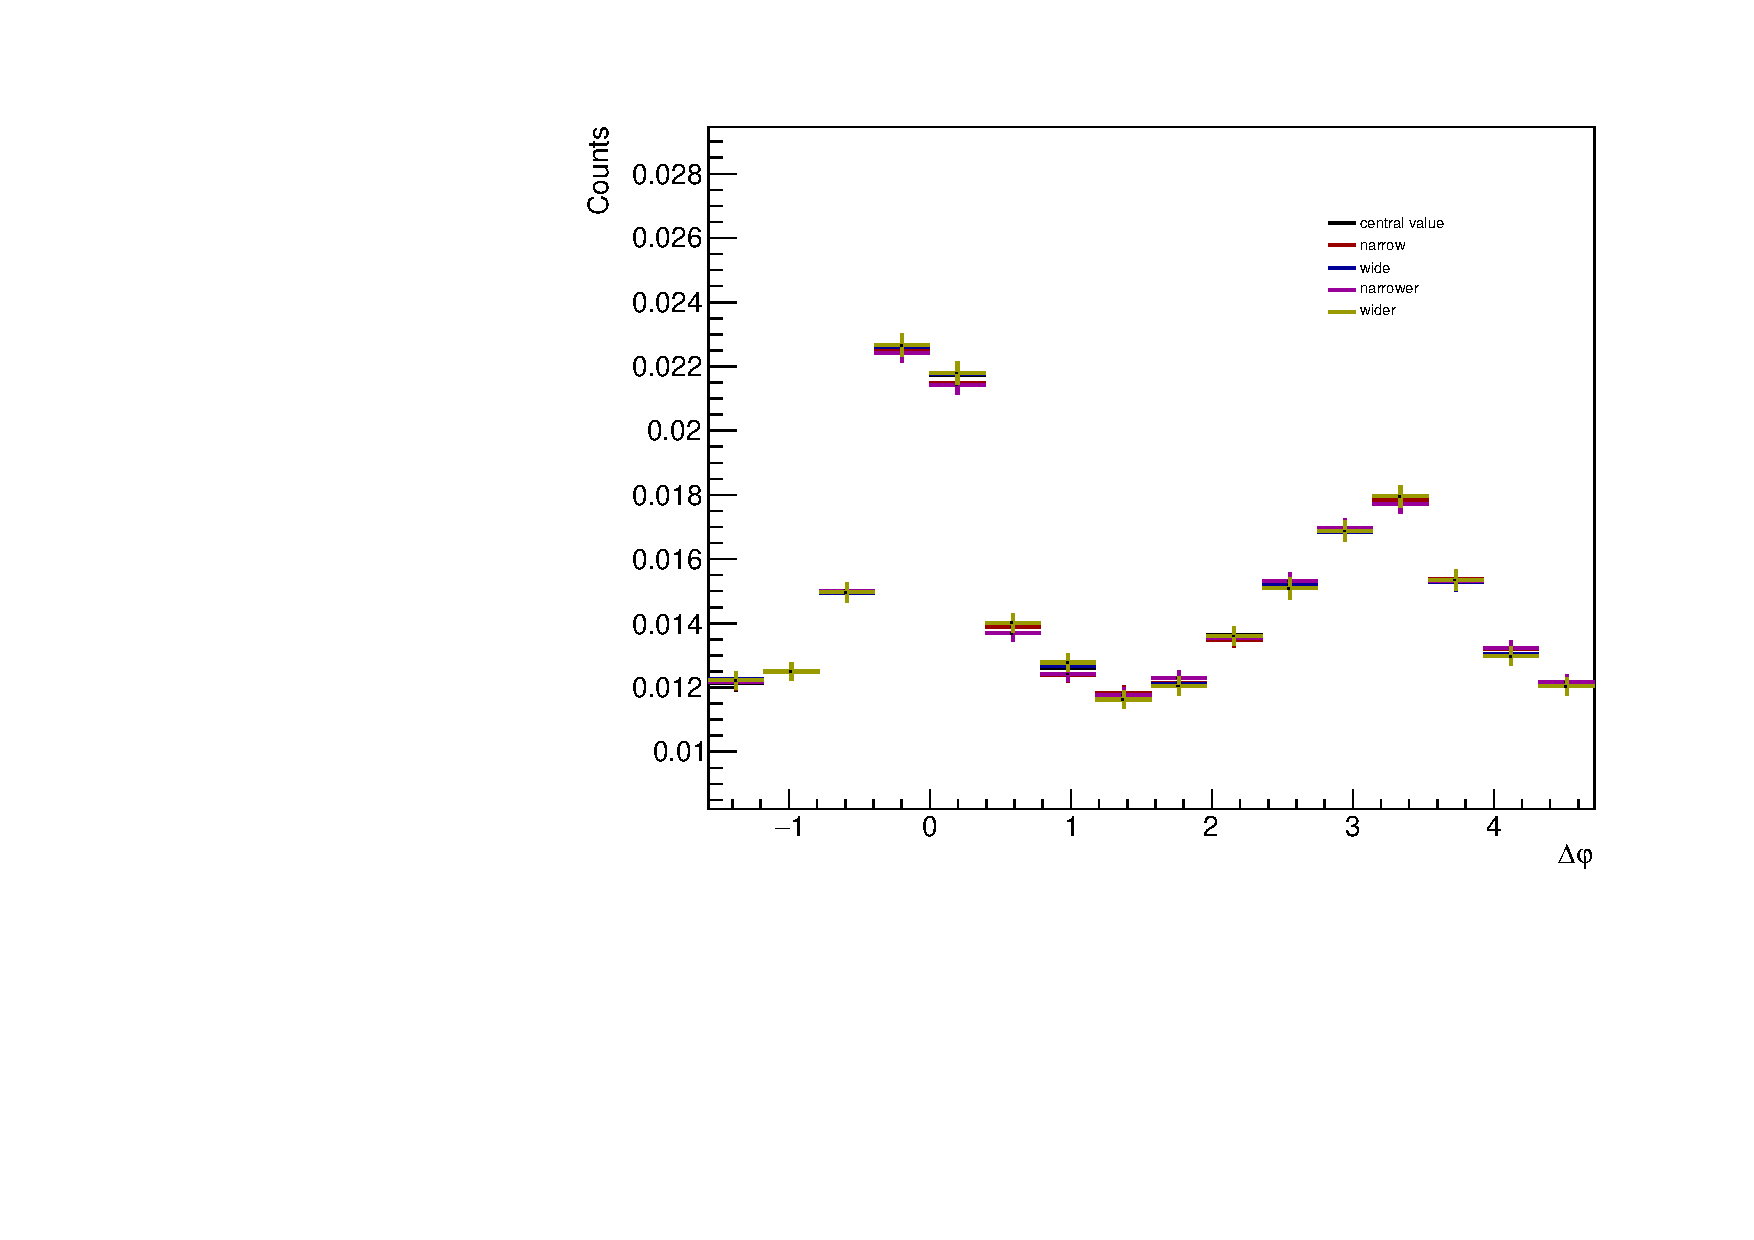
\includegraphics[width=3in]{figures/signal_variations_dphi_50_80.pdf}}
% \end{subfigure}
% \begin{subfigure}{
% 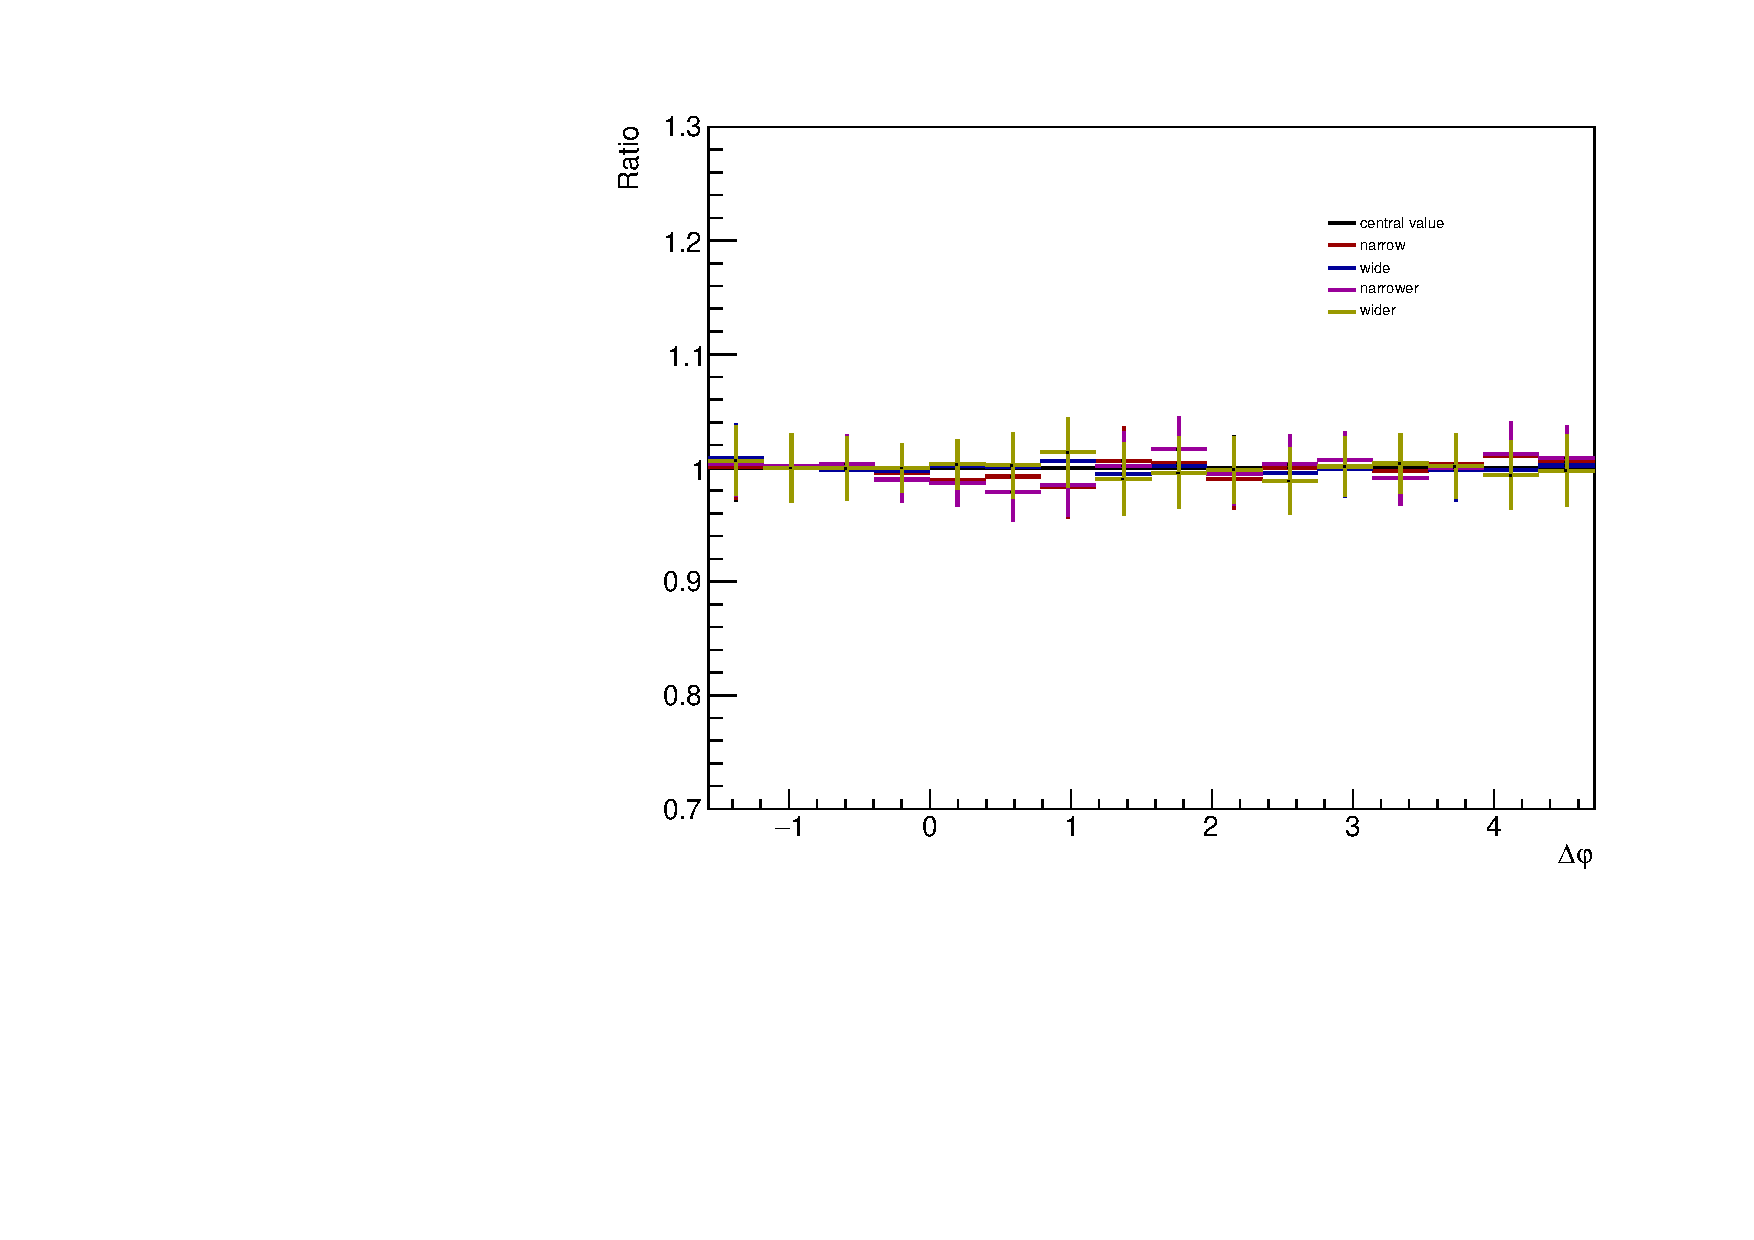
\includegraphics[width=3in]{figures/signal_variations_dphi_50_80_ratio.pdf}}
% \end{subfigure}
% \caption{The $\Delta\varphi$ distributions (left) and corresponding ratios to our central distribution (right) within the 50-80\% multiplicity bin for each of the signal region variations. We observe no dependence on the choice of signal region}
% \label{signal_region_variation_50_80}
% \end{figure}

% \subsubsection{Sideband Region Selection}
% As this analysis relies on the sideband subtraction technique, which in turn relies on our choice of sideband region, we should thoroughly investigate the effects of choosing different sideband regions on our final results. To do this, we vary the sideband region in the following ways:

% \begin{itemize}
% \item $1.135 M_{p\pi} < 1.16$ GeV/$c^2$ (wider)
% \item $1.135 < M_{p\pi} < 1.145$ GeV/$c^2$ (more narrow)
% \item $1.14 < M_{p\pi} < 1.155$ GeV/$c^2$ (shifted right)
% \item $1.086 < M_{p\pi} < 1.098$ GeV/$c^2$ (shifted left (on other side of signal region))
% \end{itemize}

% The resulting $\Delta\varphi$ distributions and ratios to central values for each sideband region variation in each multiplicity bin within our central $p_{T, assoc}$ bin are shown in Figures \ref{sideband_region_variation_0_20} through \ref{sideband_region_variation_50_80}. As we observe no dependence on $\Delta\varphi$, the systematic is calculated as the RMS of the ratios of within the entire $\Delta\varphi$ range for each variation.

% \begin{figure}[ht]
% \centering
% \begin{subfigure}{
% 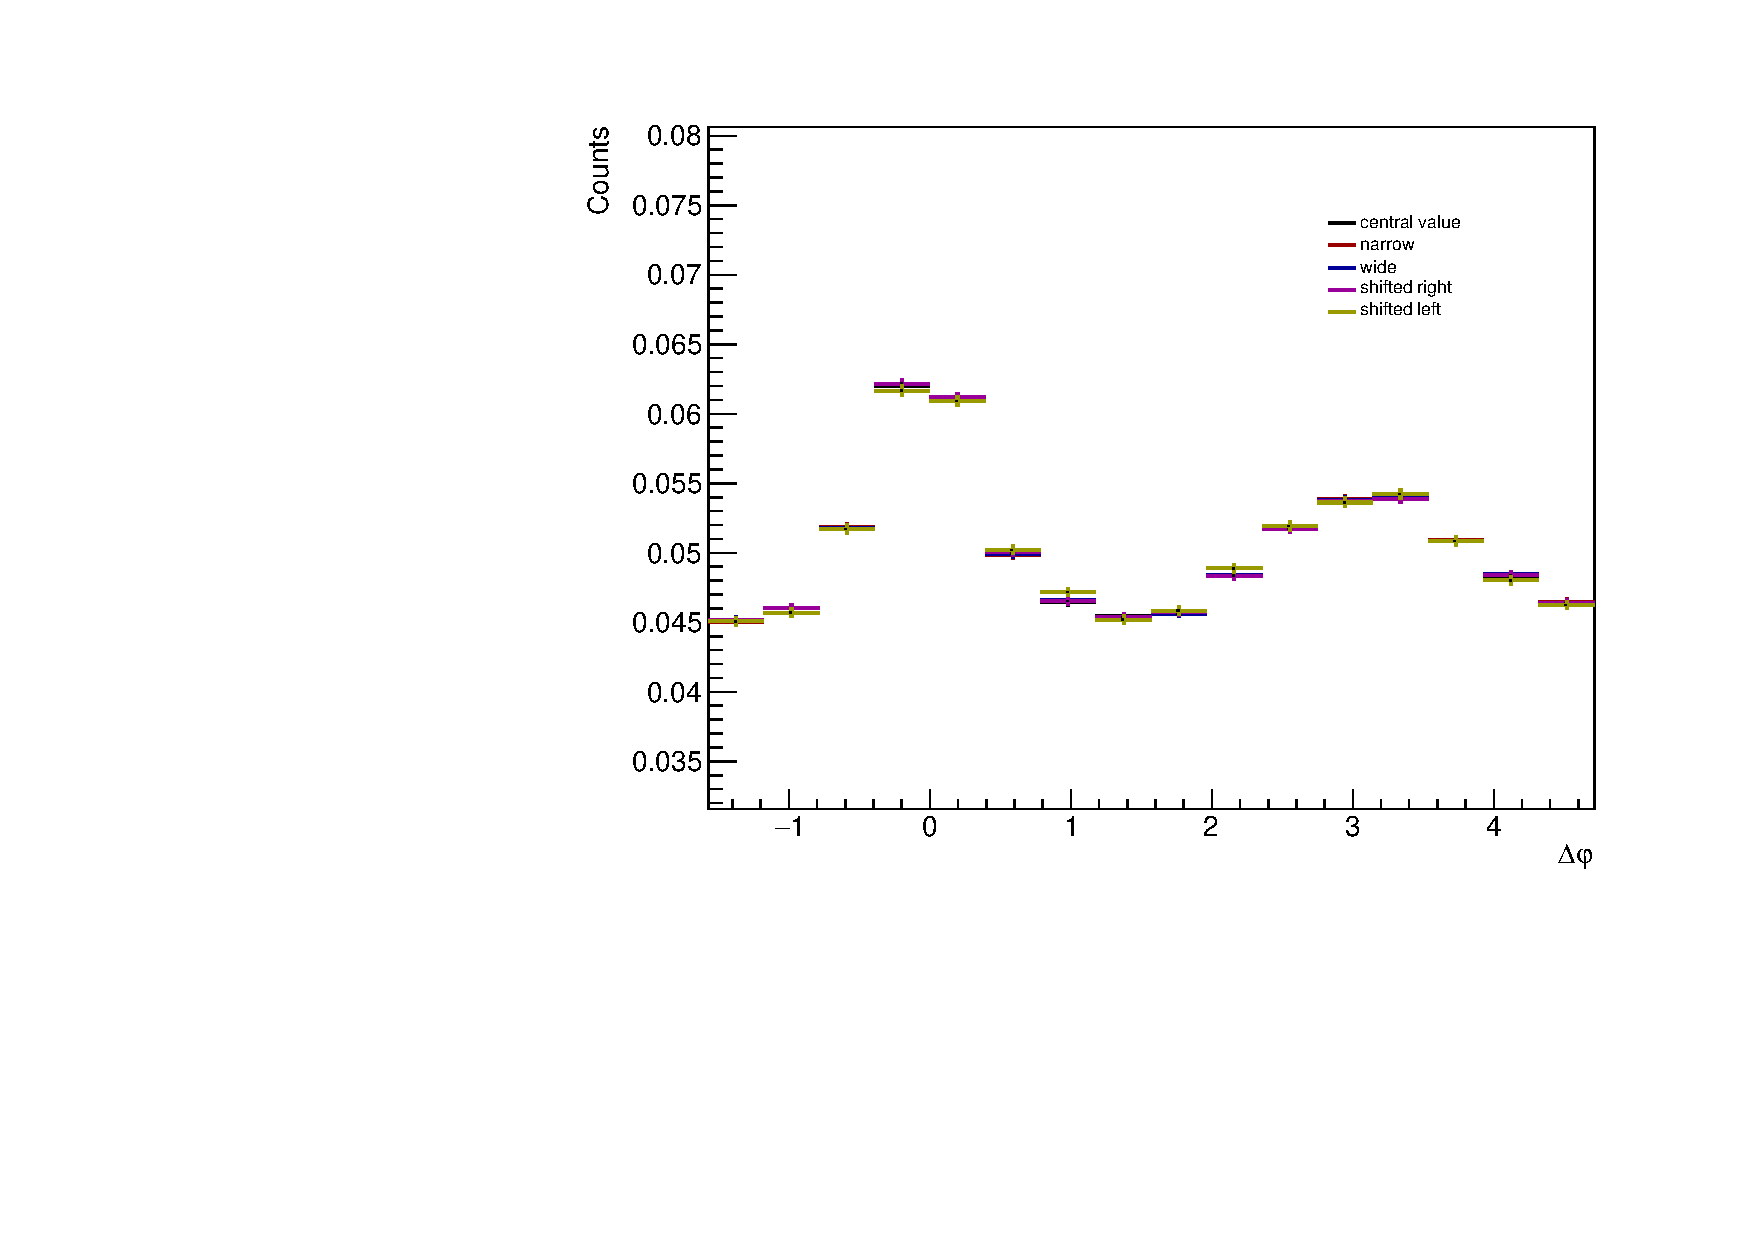
\includegraphics[width=3in]{figures/sideband_variations_dphi_0_20.pdf}}
% \end{subfigure}
% \begin{subfigure}{
% 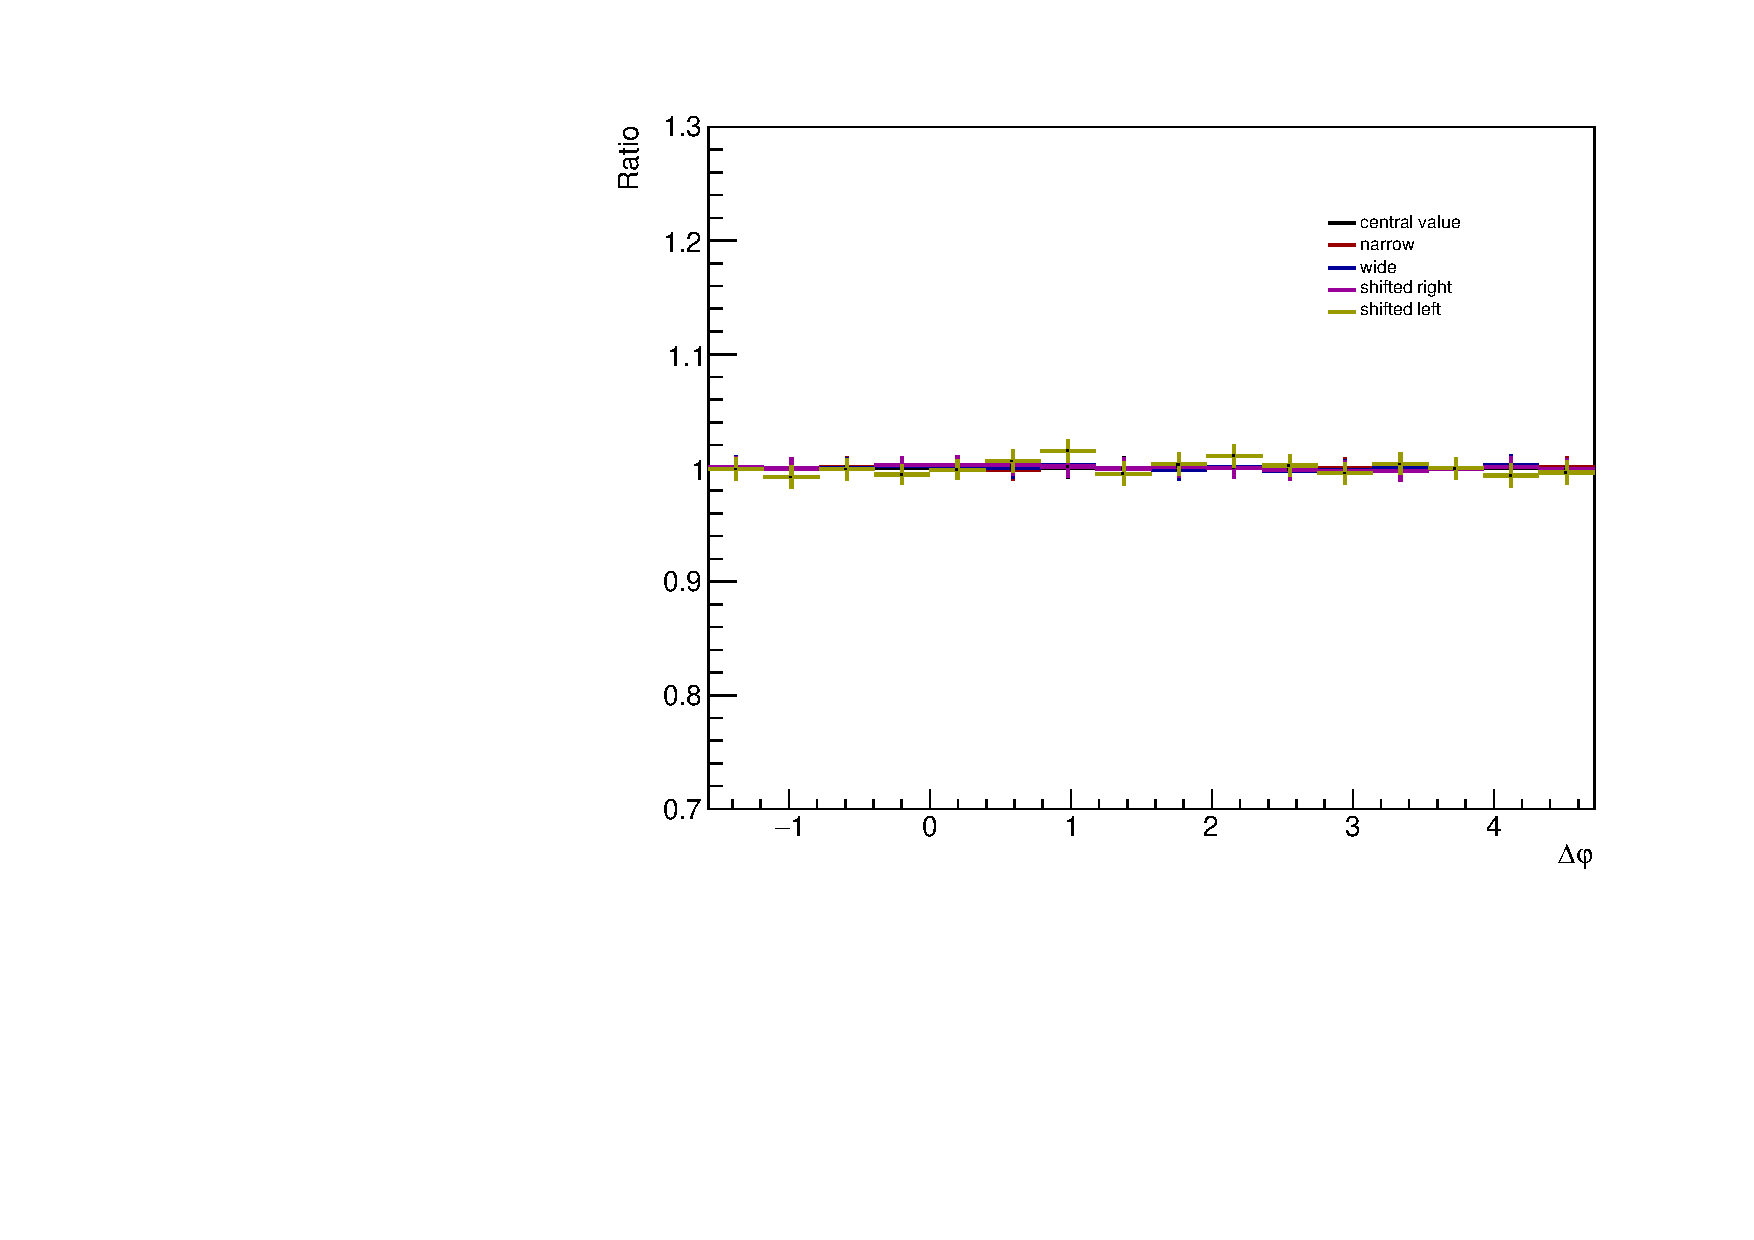
\includegraphics[width=3in]{figures/sideband_variations_dphi_0_20_ratio.pdf}}
% \end{subfigure}
% \caption{The $\Delta\varphi$ distributions (left) and corresponding ratios to our central distribution (right) within the 0-20\% multiplicity bin for each of the sideband region variations. We observe no dependence on the choice of sideband region}
% \label{sideband_region_variation_0_20}

% \end{figure}
% \begin{figure}[ht]
% \centering
% \begin{subfigure}{
% 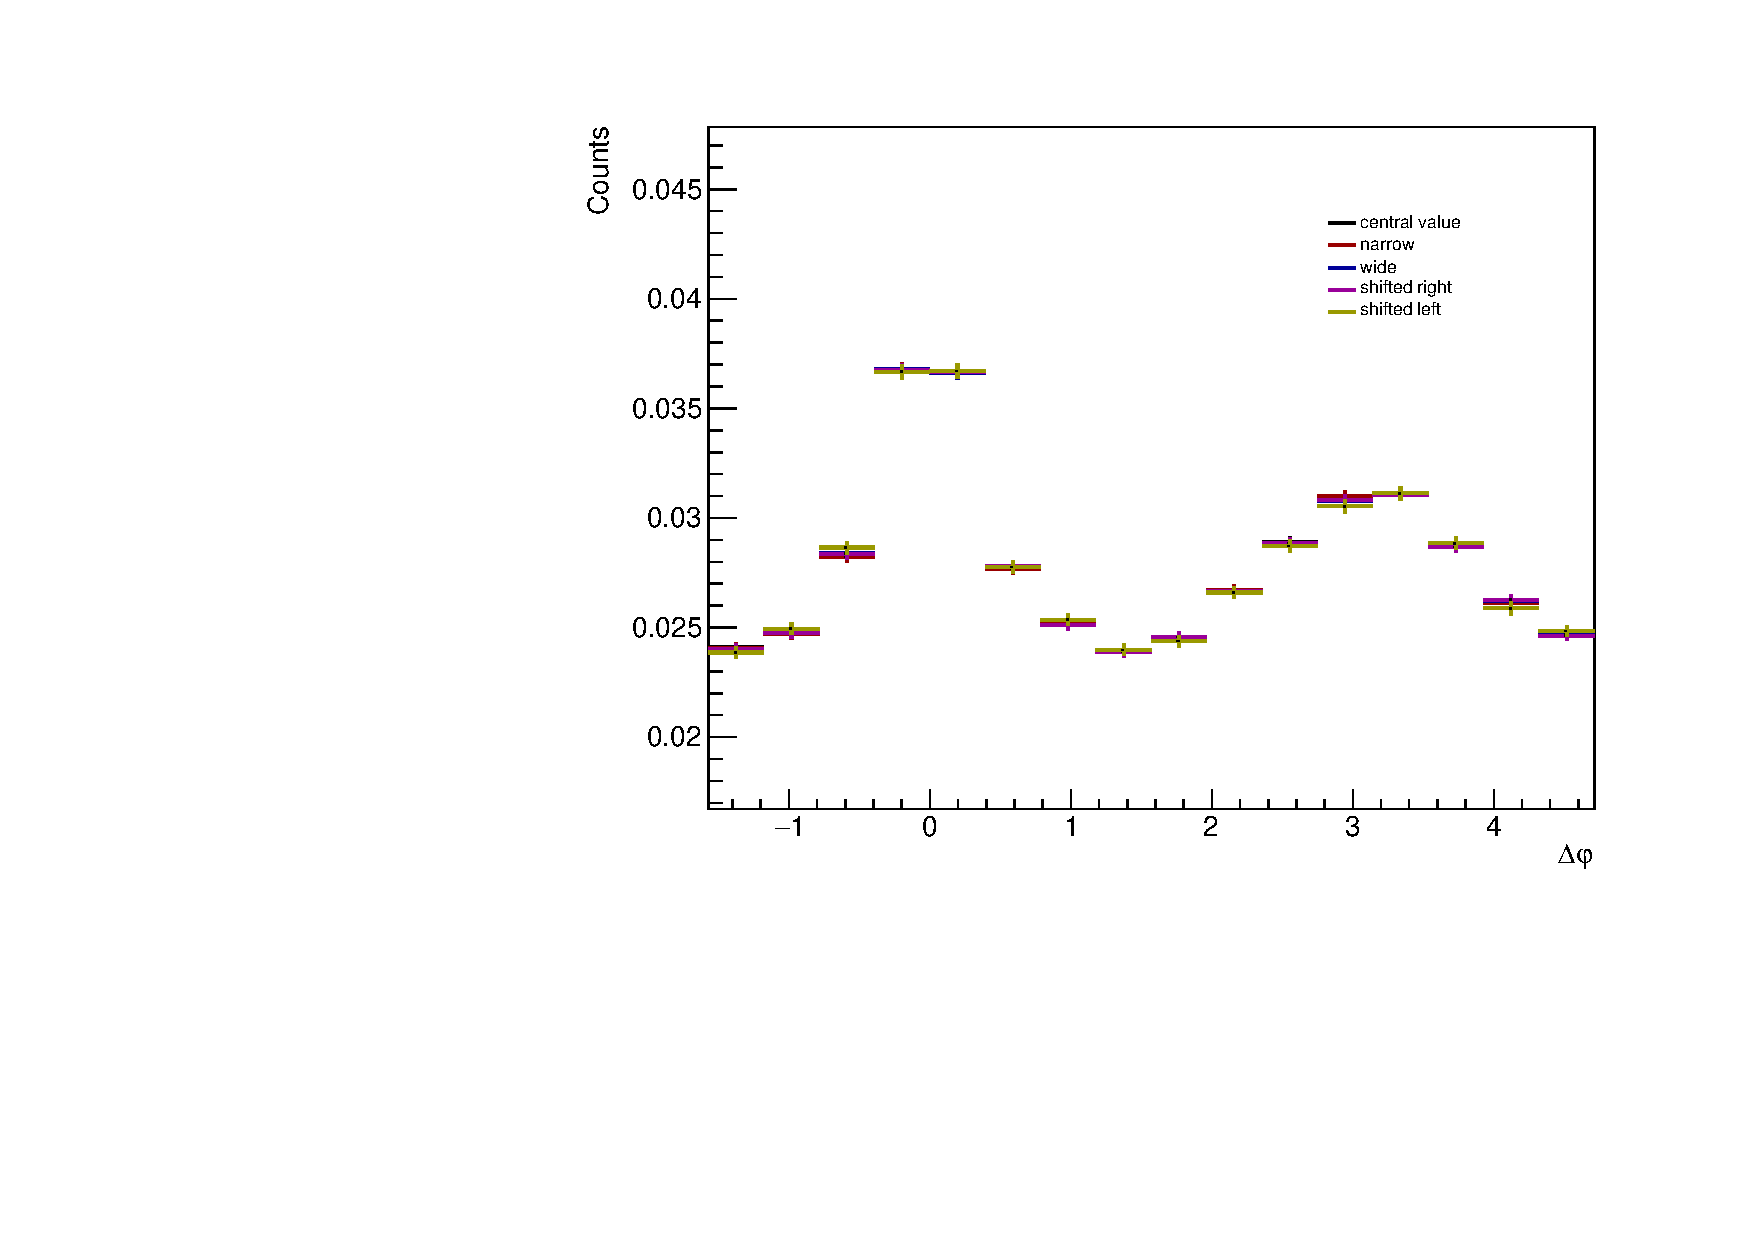
\includegraphics[width=3in]{figures/sideband_variations_dphi_20_50.pdf}}
% \end{subfigure}
% \begin{subfigure}{
% 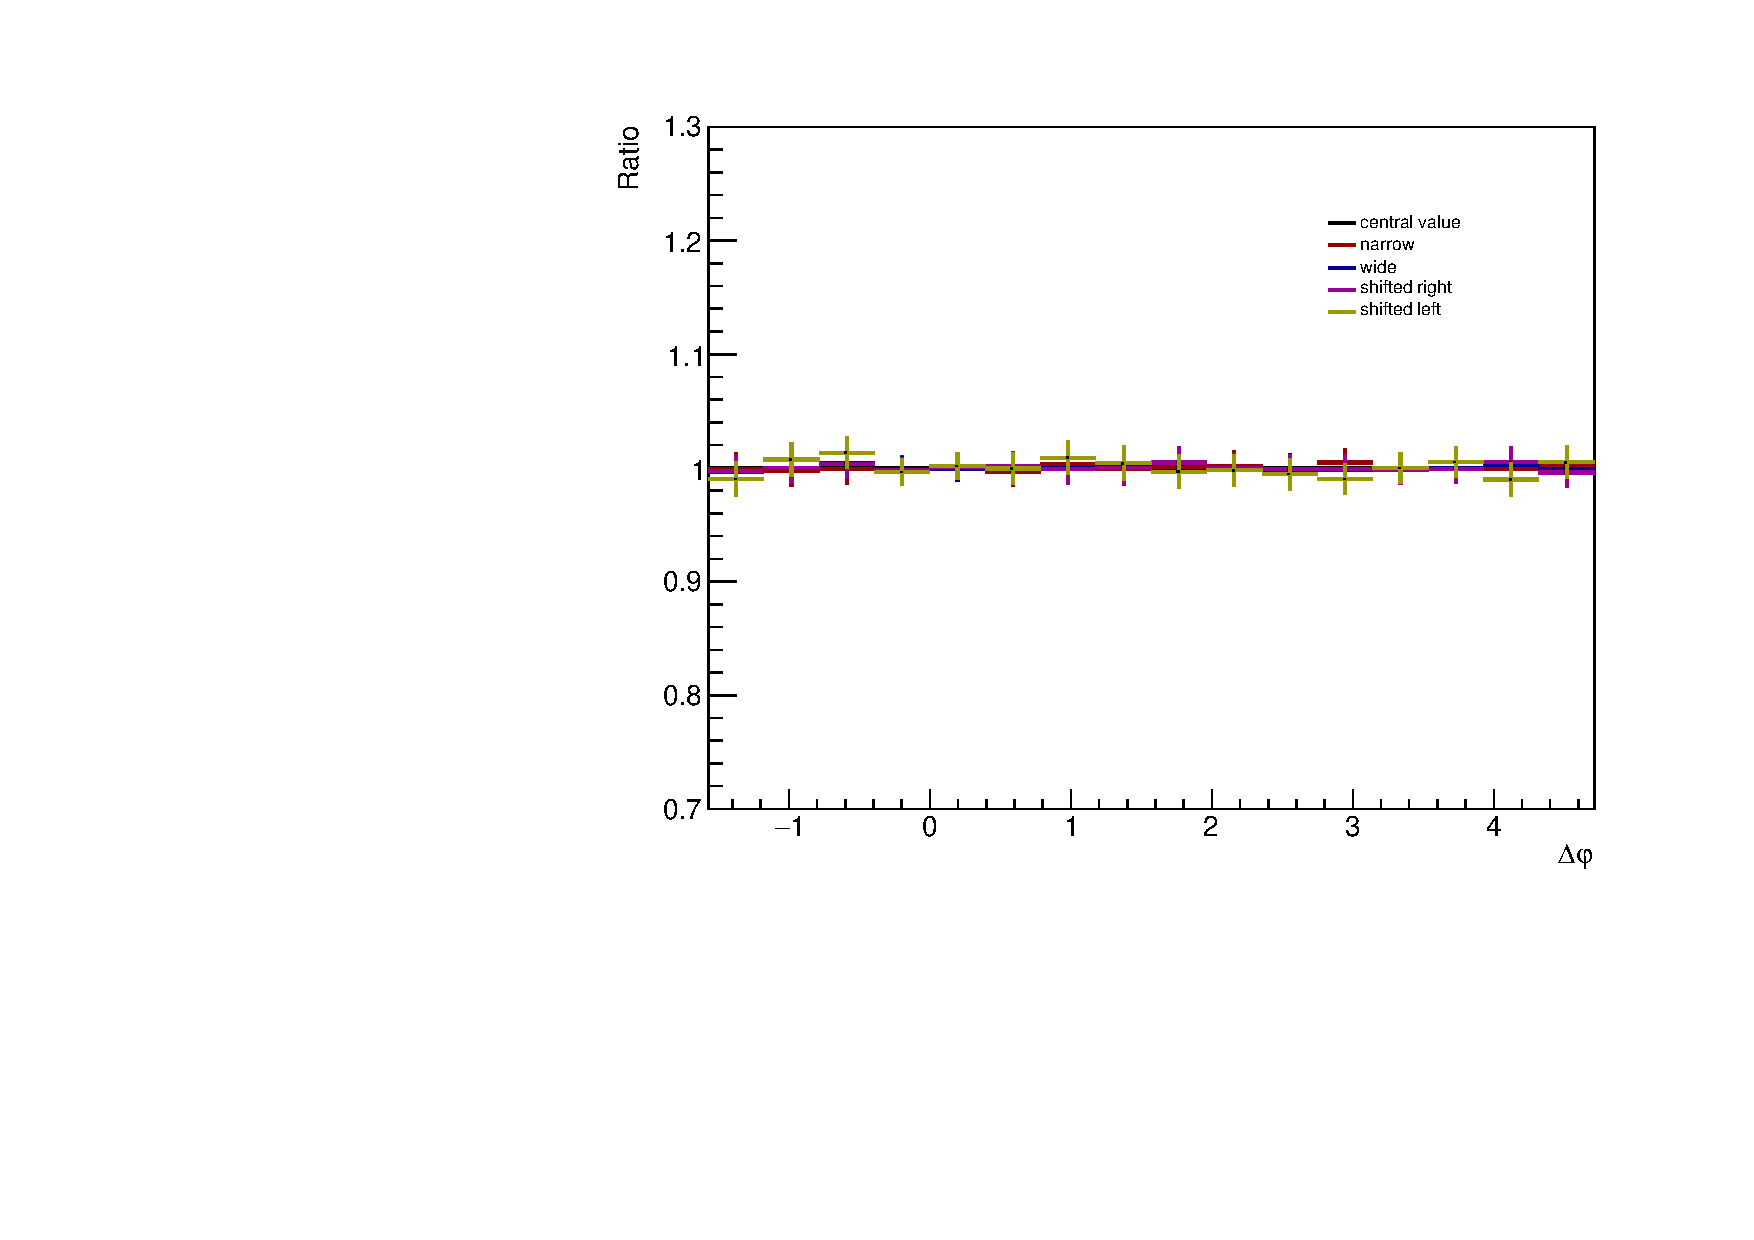
\includegraphics[width=3in]{figures/sideband_variations_dphi_20_50_ratio.pdf}}
% \end{subfigure}
% \caption{The $\Delta\varphi$ distributions (left) and corresponding ratios to our central distribution (right) within the 20-50\% multiplicity bin for each of the sideband region variations. We observe no dependence on the choice of sideband region}
% \label{sideband_region_variation_20_50}
% \end{figure}

% \begin{figure}[ht]
% \centering
% \begin{subfigure}{
% 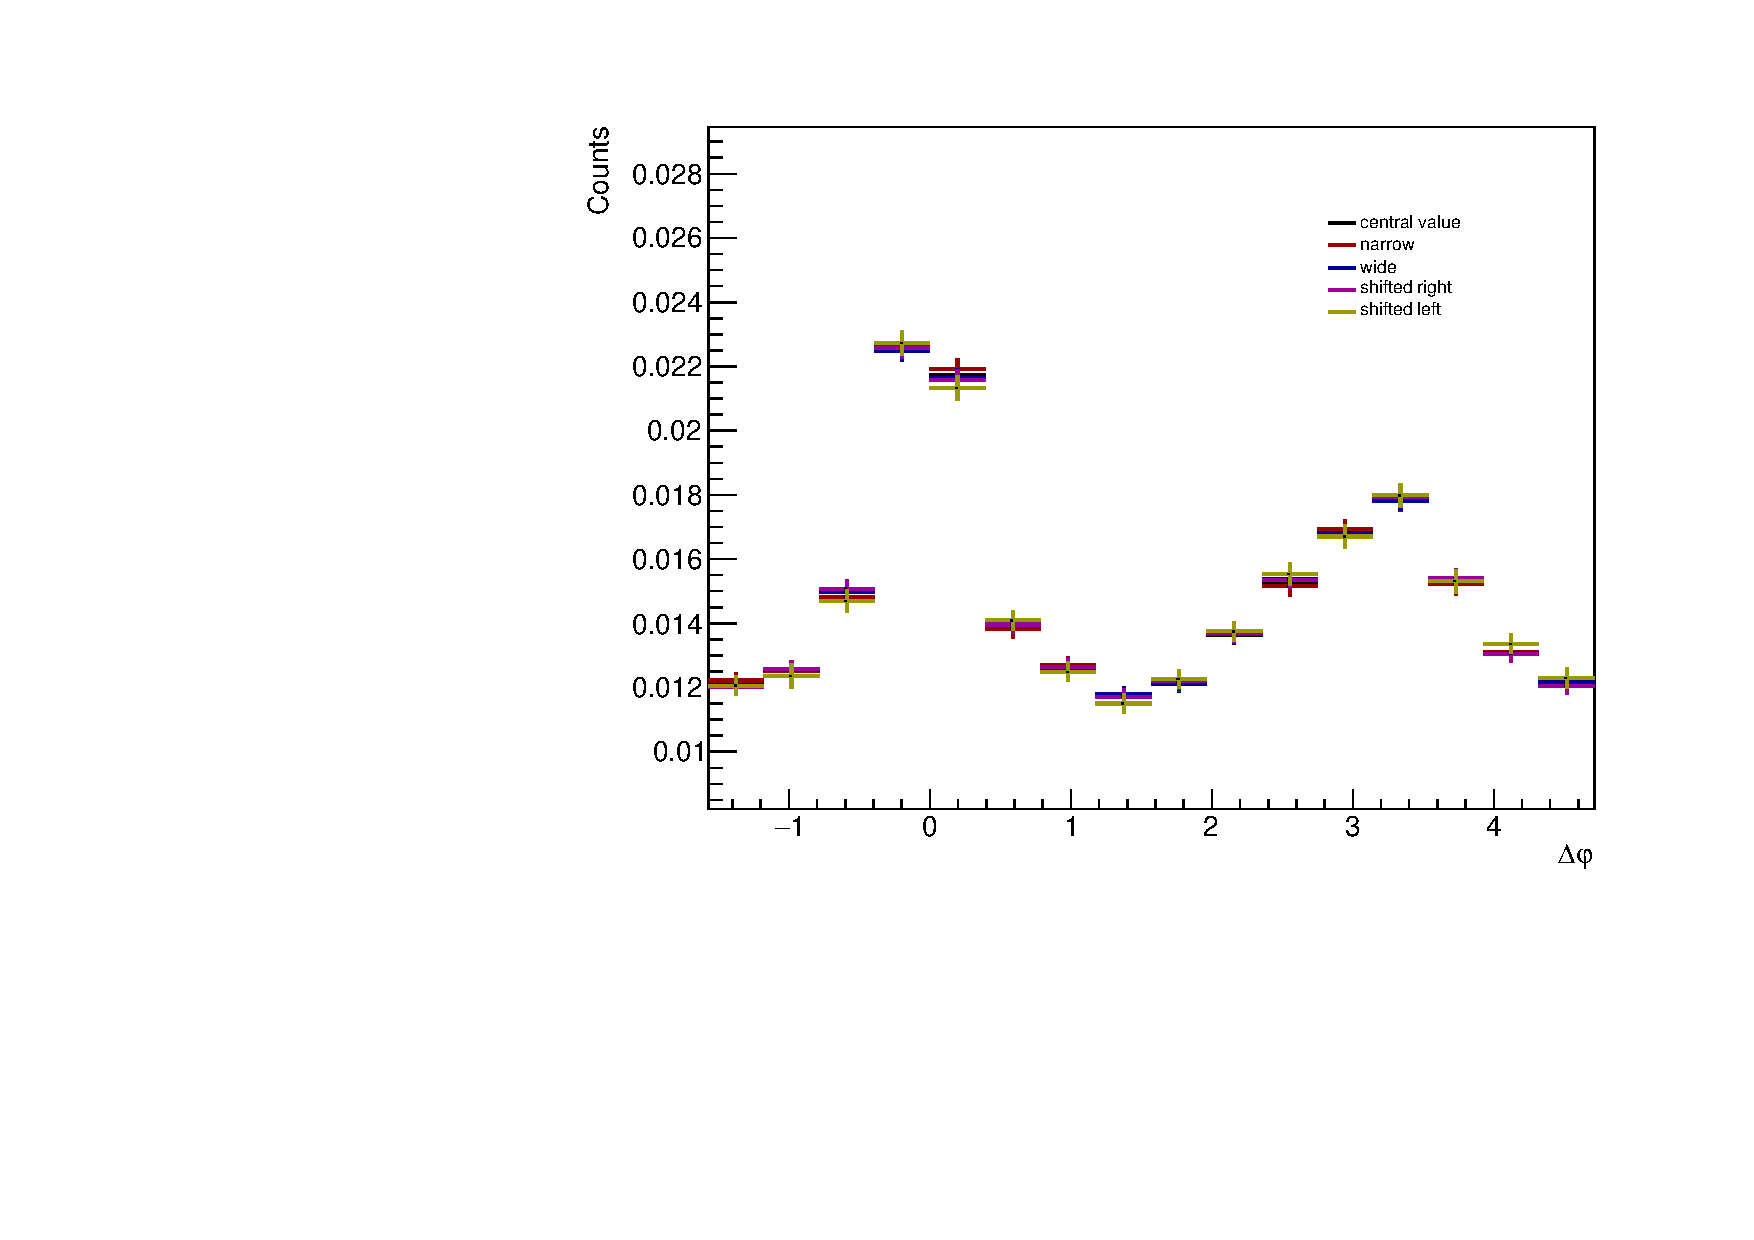
\includegraphics[width=3in]{figures/sideband_variations_dphi_50_80.pdf}}
% \end{subfigure}
% \begin{subfigure}{
% 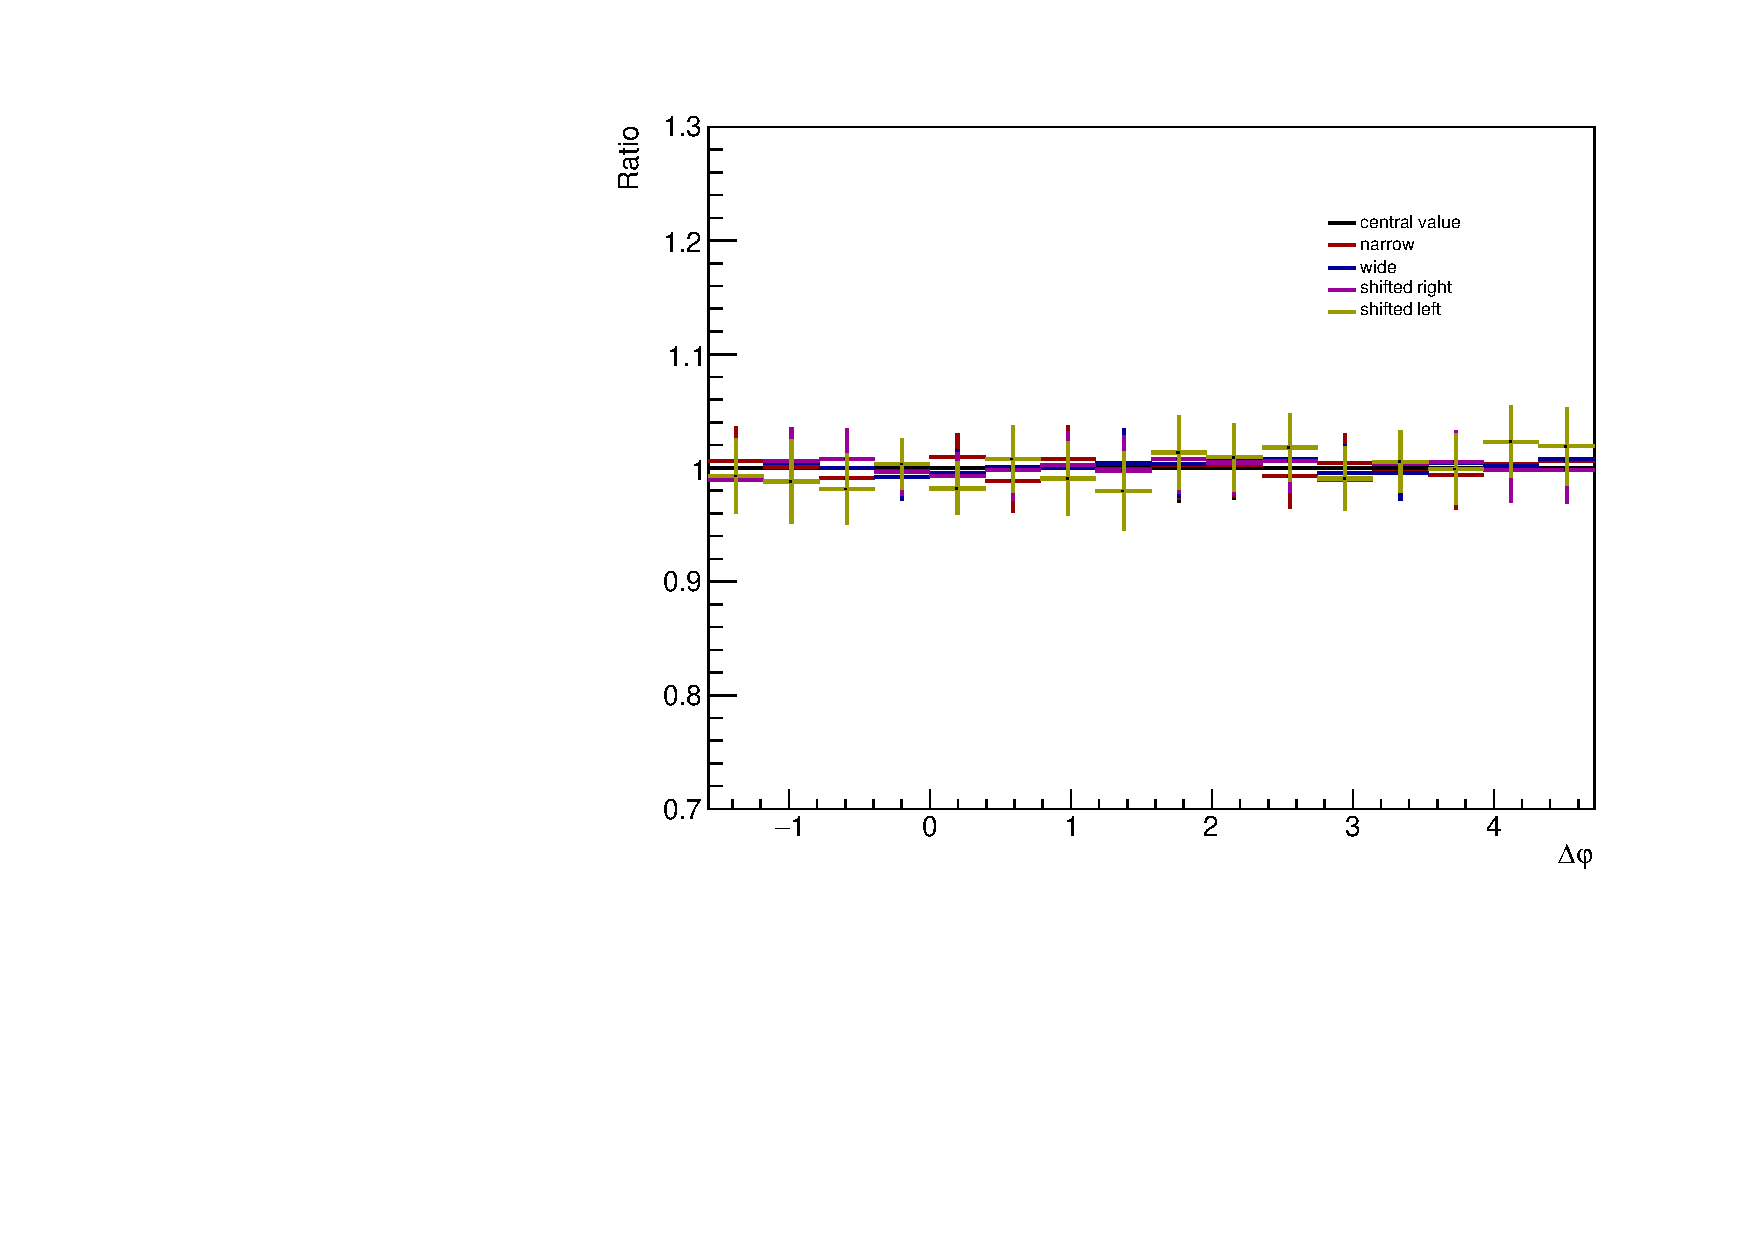
\includegraphics[width=3in]{figures/sideband_variations_dphi_50_80_ratio.pdf}}
% \end{subfigure}
% \caption{The $\Delta\varphi$ distributions (left) and corresponding ratios to our central distribution (right) within the 50-80\% multiplicity bin for each of the sideband region variations. We observe no dependence on the choice of sideband region}
% \label{sideband_region_variation_50_80}
% \end{figure}

% \subsubsection{PID Cut Selection}
% While there appears to be no contamination present in either our daughter proton or pion PID distributions from Section \ref{v0_daughter_pid}, we still investigate the effects of varying our PID cuts for both the proton and pion. The PID cuts are varied in the following ways:

% \begin{itemize}
% \item $|n\sigma_{TPC, TOF}^{p}| < 2.8$, $|n\sigma_{TPC, TOF}^{\pi}| < 4.2$ (40\% more wide, veto cut on TOF)
% \item $|n\sigma_{TPC, TOF}^{p}| < 1.2$, $|n\sigma_{TPC,TOF}^{\pi}| < 1.8$ (40\% more narrow, veto cut on TOF)
% \item $|n\sigma_{TPC, TOF}^{p}| < 2.0$, $|n\sigma_{TPC,TOF}^{\pi}| < 3.0$ (same width, require TOF hit)
% \end{itemize}

% The resulting $\Delta\varphi$ distributions and ratios to central values for each PID cut variation in each multiplicity bin within our central $p_{T, assoc}$ bin are shown in Figures \ref{pid_cut_variation_0_20} through \ref{pid_cut_variation_50_80}. We observe that requiring a TOF hit has a slight systematic effect on the $\Delta\varphi$ distribution, but we still include this variation in our systematic calculation. As we observe no dependence on $\Delta\varphi$, the systematic is calculated as the RMS of the ratios of within the entire $\Delta\varphi$ range for each variation.

% \begin{figure}[ht]
% \centering
% \begin{subfigure}{
% 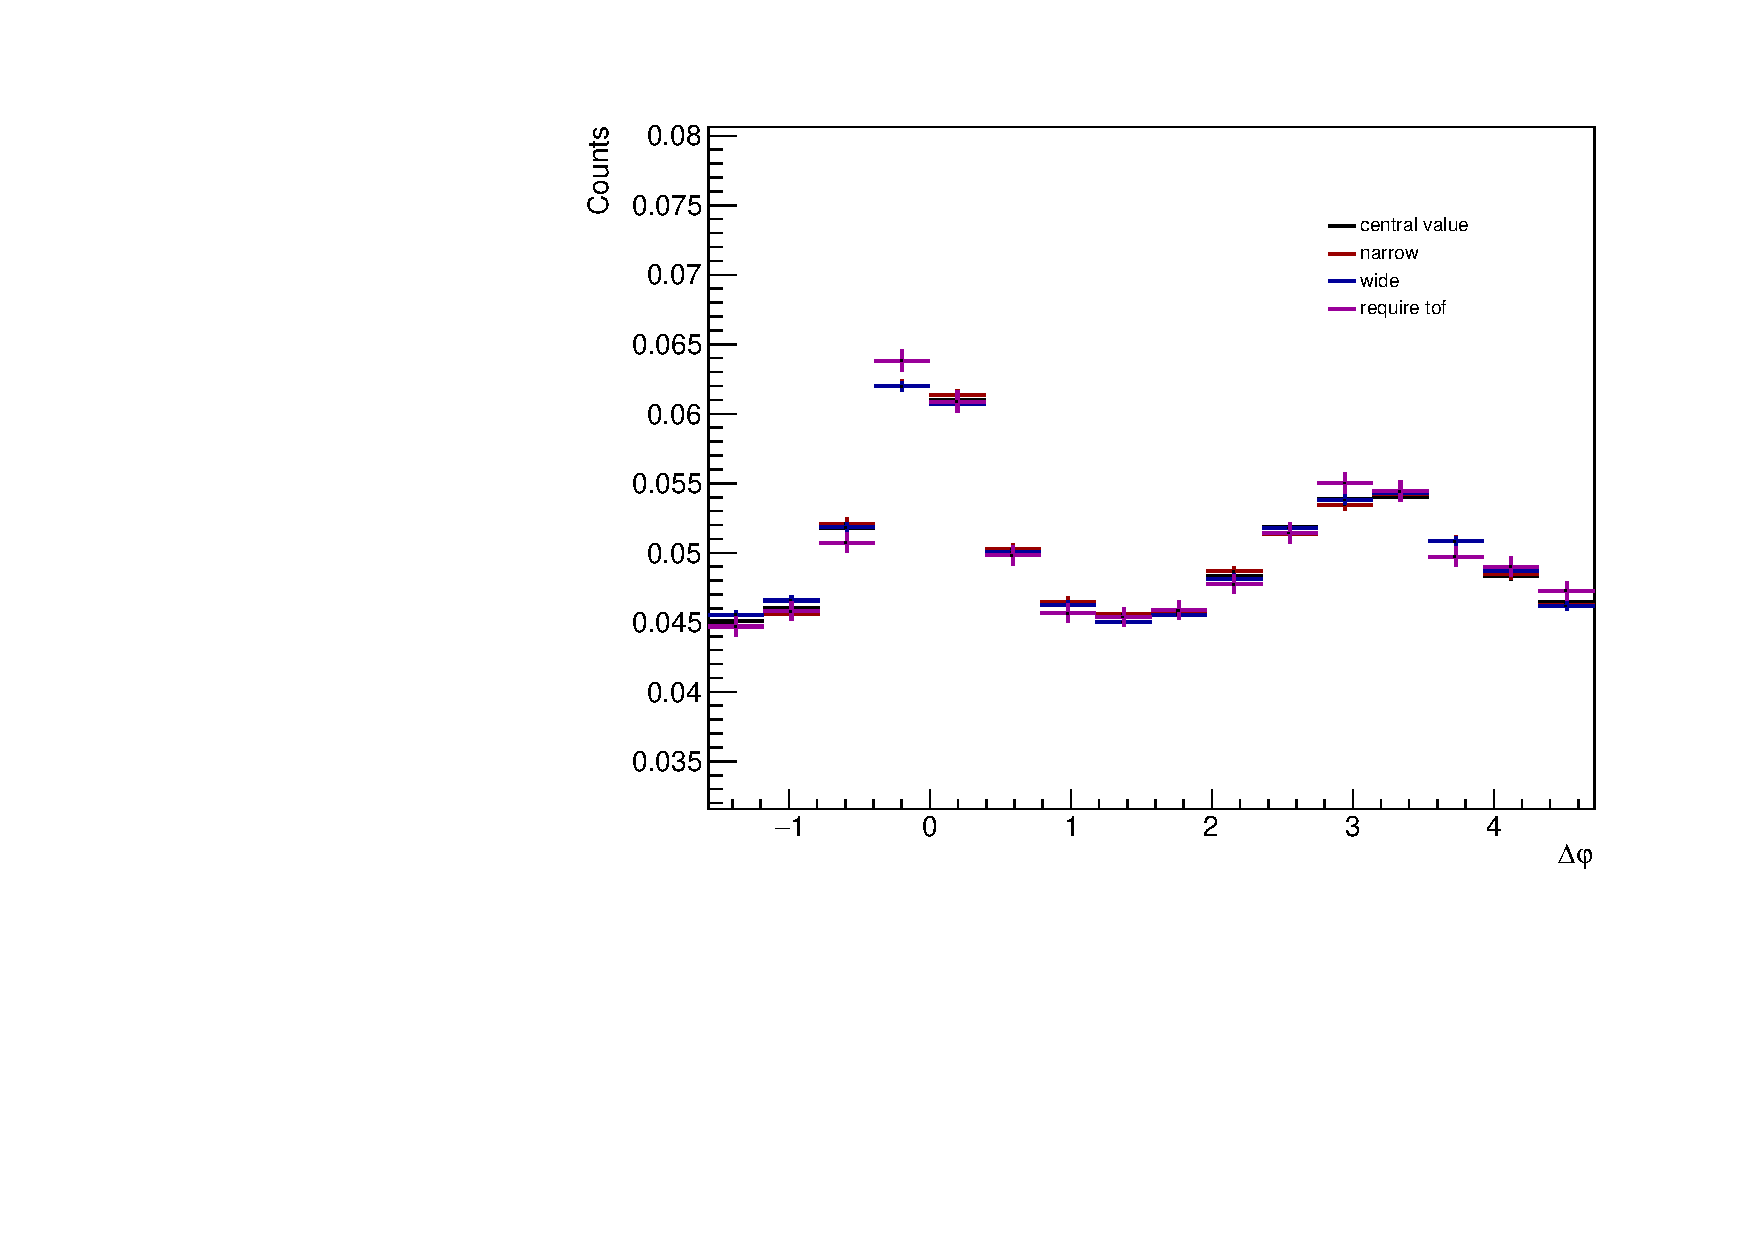
\includegraphics[width=3in]{figures/pid_variations_dphi_0_20.pdf}}
% \end{subfigure}
% \begin{subfigure}{
% 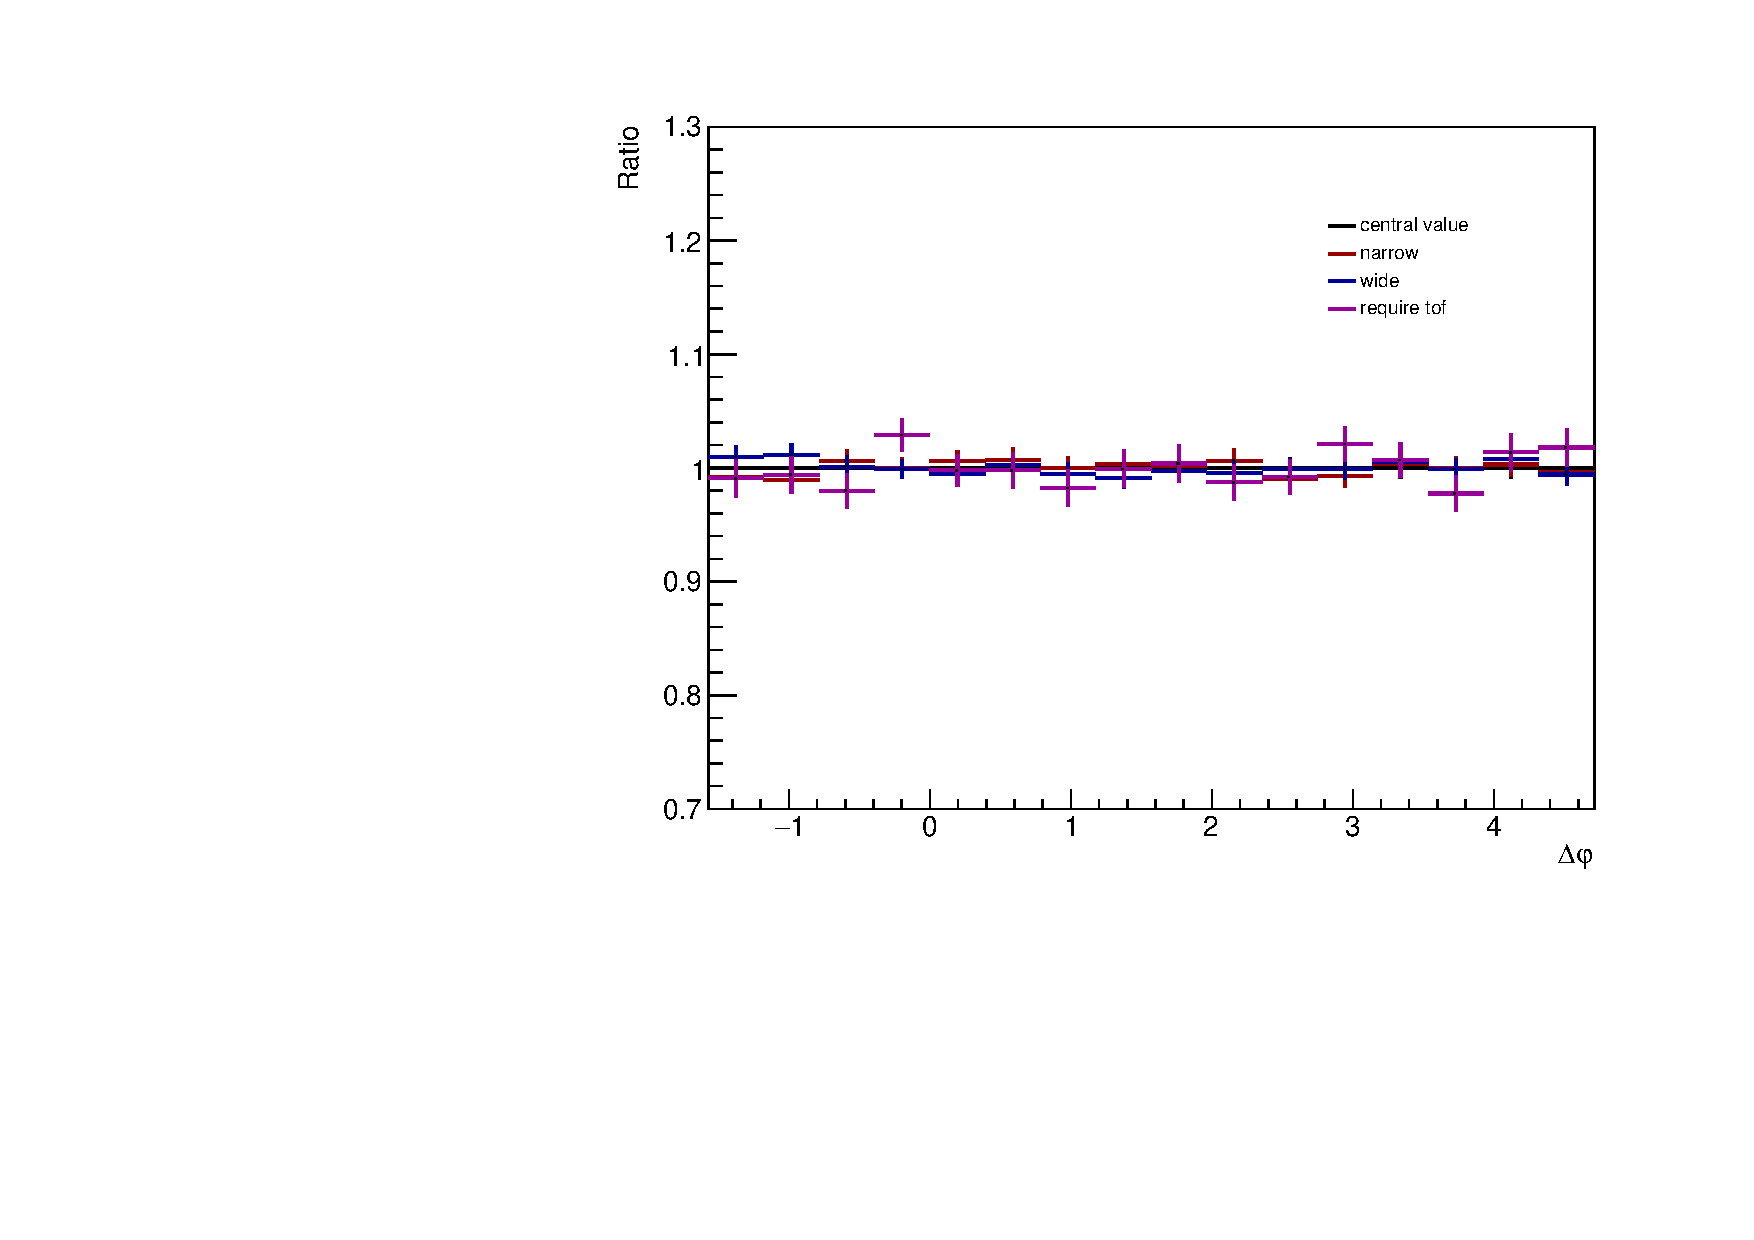
\includegraphics[width=3in]{figures/pid_variations_dphi_0_20_ratio.pdf}}
% \end{subfigure}
% \caption{The $\Delta\varphi$ distributions (left) and corresponding ratios to our central distribution (right) within the 0-20\% multiplicity bin for each of the PID cut variations. We observe no dependence on the choice of PID cuts.}
% \label{pid_cut_variation_0_20}
% \end{figure}

% \begin{figure}[ht]
% \centering
% \begin{subfigure}{
% 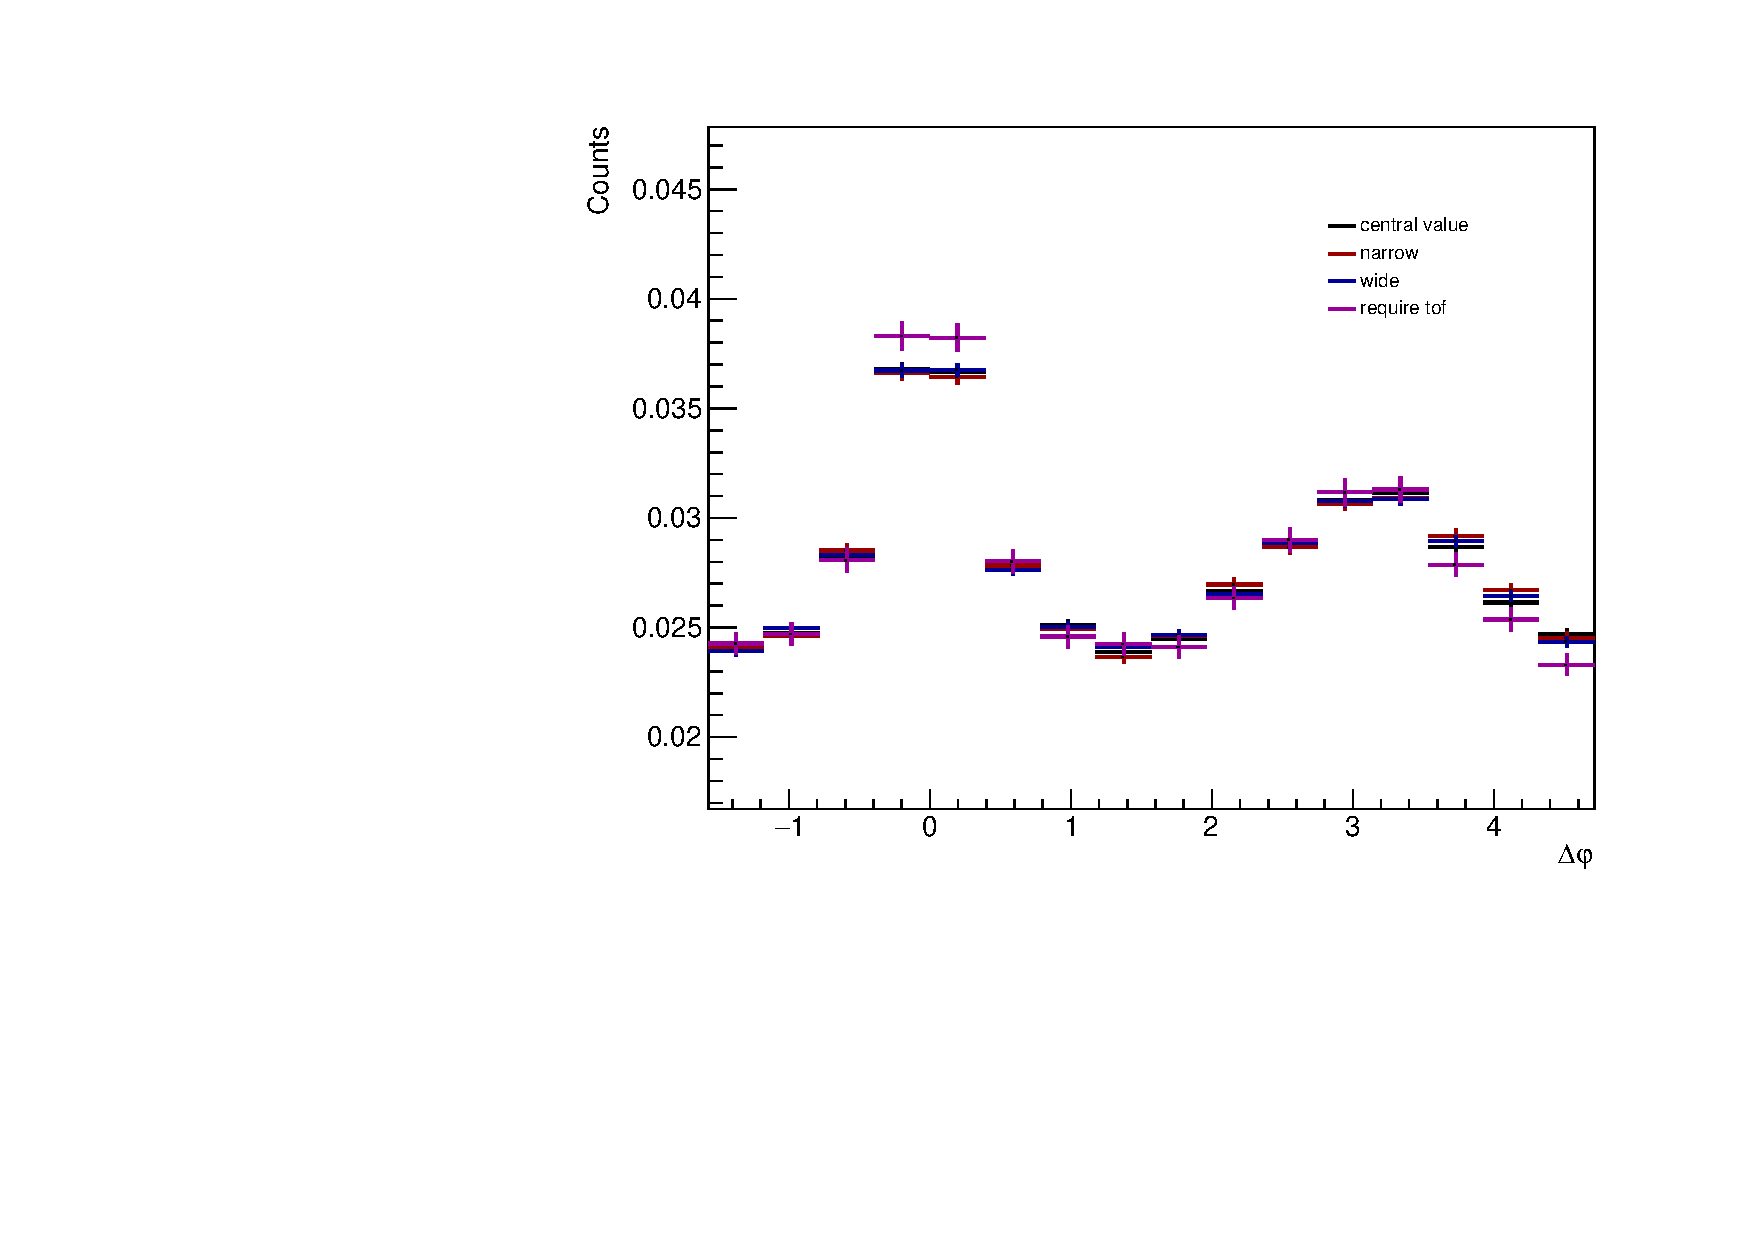
\includegraphics[width=3in]{figures/pid_variations_dphi_20_50.pdf}}
% \end{subfigure}
% \begin{subfigure}{
% 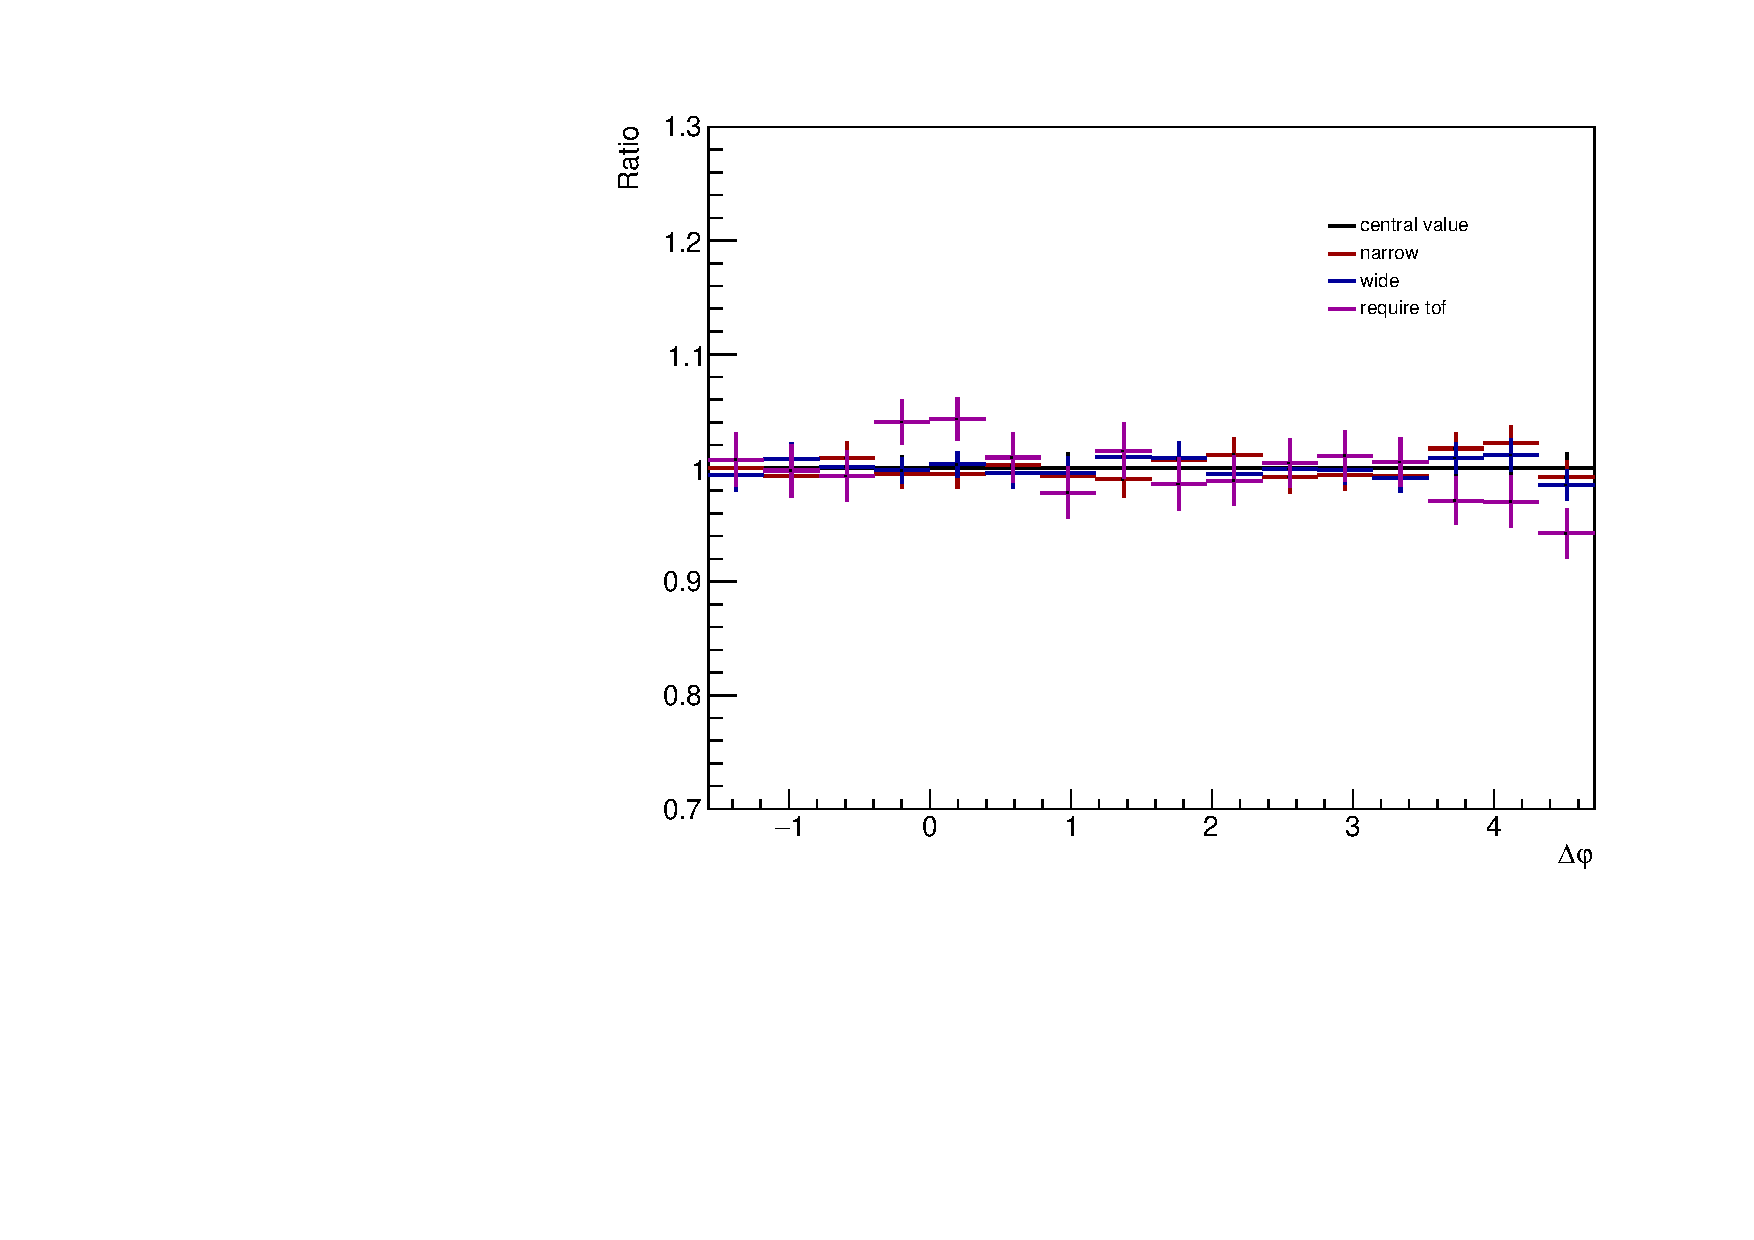
\includegraphics[width=3in]{figures/pid_variations_dphi_20_50_ratio.pdf}}
% \end{subfigure}
% \caption{The $\Delta\varphi$ distributions (left) and corresponding ratios to our central distribution (right) within the 20-50\% multiplicity bin for each of the PID cut variations. We observe no dependence on the choice of PID cuts.}
% \label{pid_cut_variation_20_50}
% \end{figure}

% \clearpage

% \begin{figure}[ht]
% \centering
% \begin{subfigure}{
% 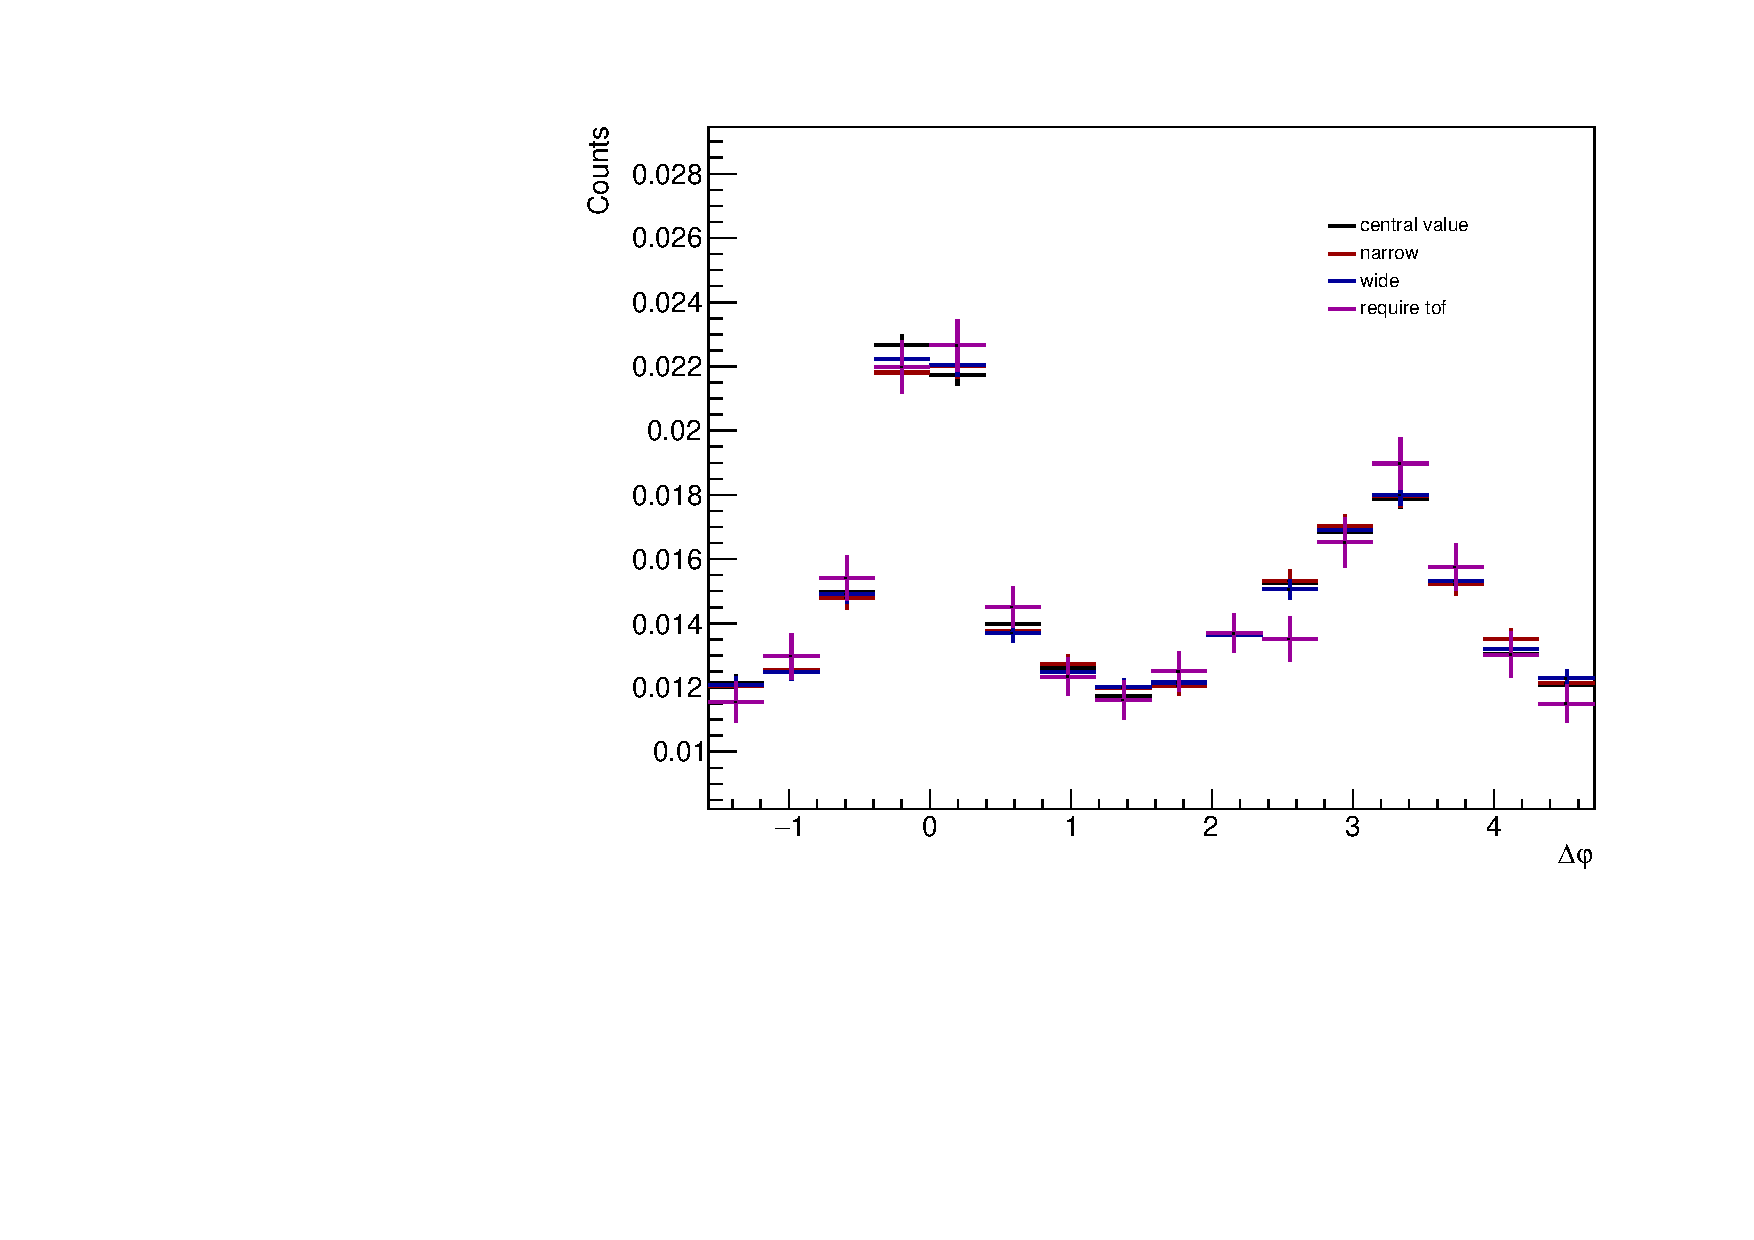
\includegraphics[width=3in]{figures/pid_variations_dphi_50_80.pdf}}
% \end{subfigure}
% \begin{subfigure}{
% 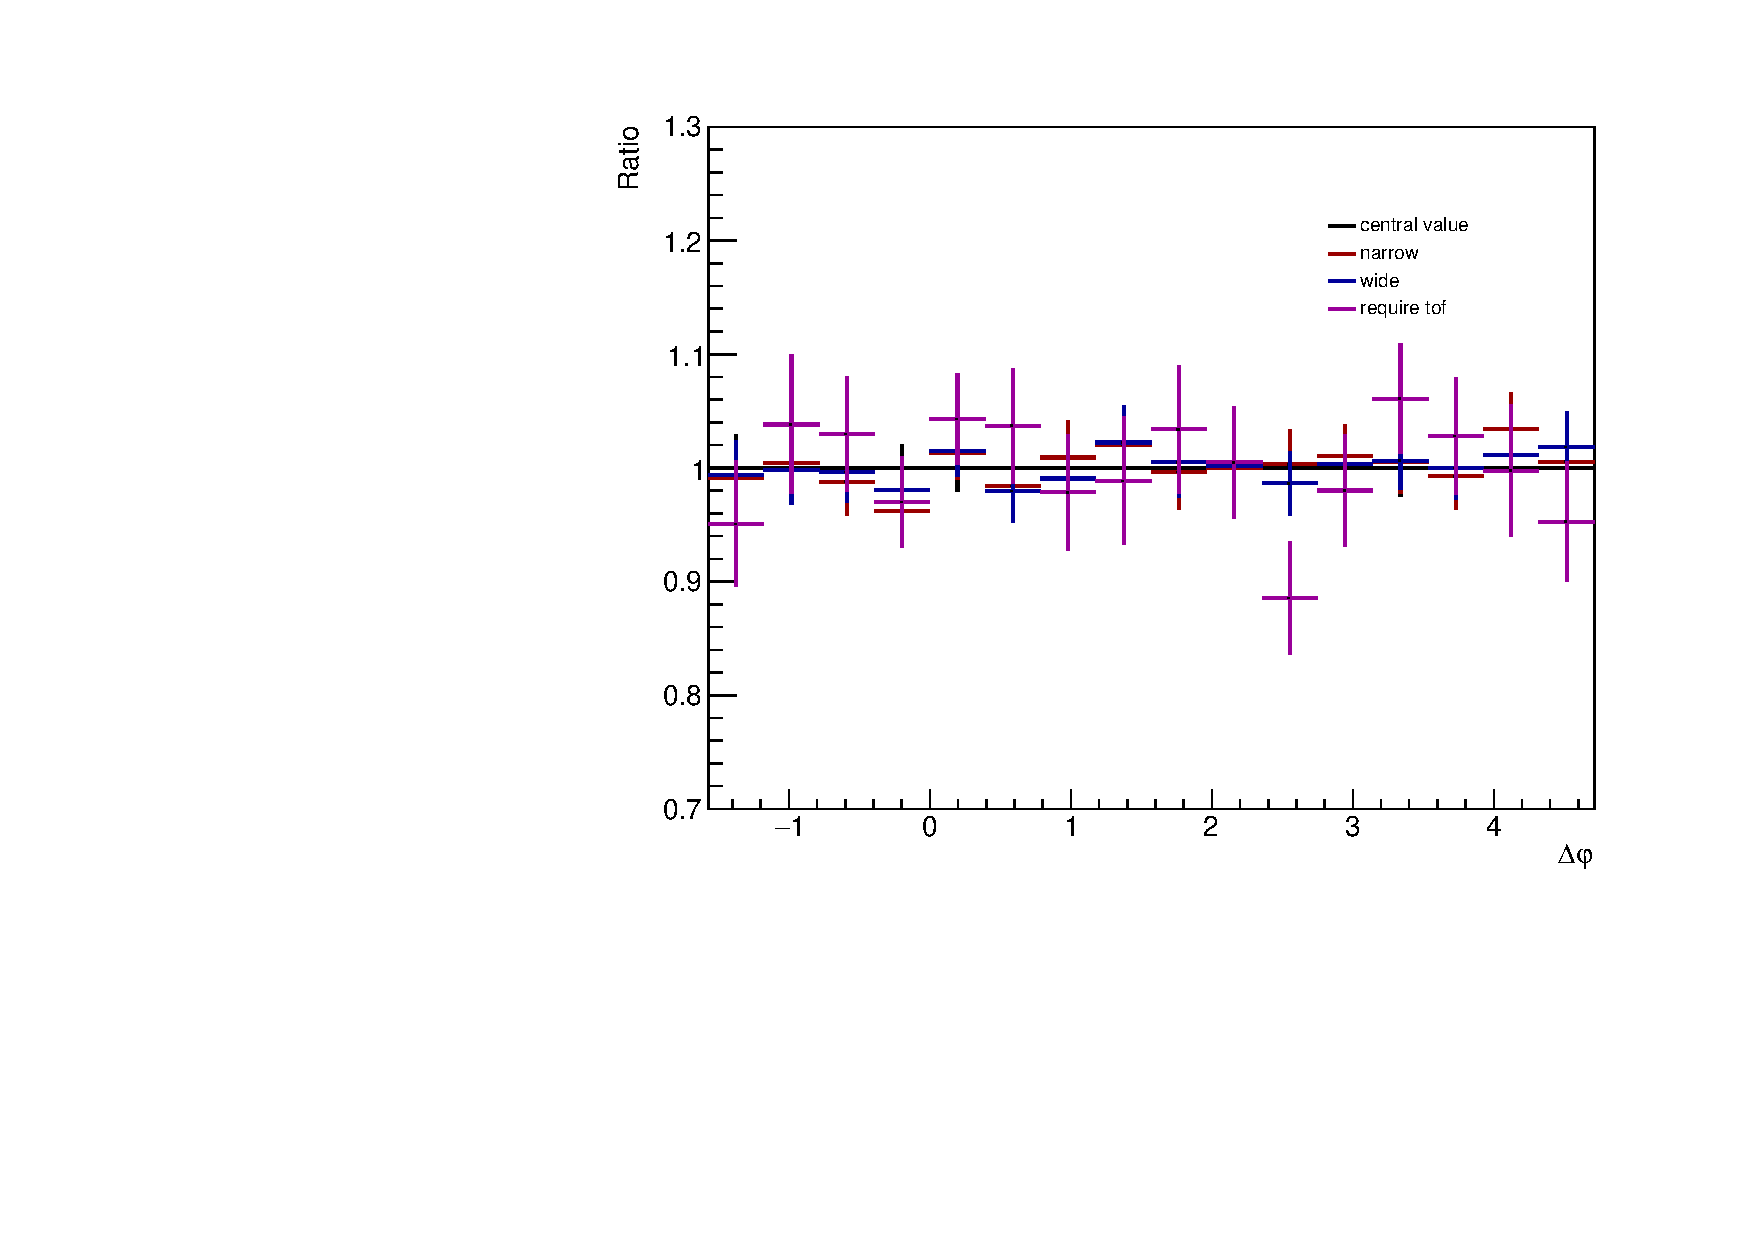
\includegraphics[width=3in]{figures/pid_variations_dphi_50_80_ratio.pdf}}
% \end{subfigure}
% \caption{The $\Delta\varphi$ distributions (left) and corresponding ratios to our central distribution (right) within the 50-80\% multiplicity bin for each of the PID cut variations. We observe no dependence on the choice of PID cuts.}
% \label{pid_cut_variation_50_80}
% \end{figure}

% \subsubsection{Barlow Check ($\Delta\varphi$ distribution generation)}
% \label{barlow_check_dphi}

% In order to ensure the variations listed above are sensible and not just variations for the sake of variations, we perform a ``standard'' Barlow check procedure (described here: \url{https://arxiv.org/abs/hep-ex/0207026}). For each $\Delta\varphi$ bin, we calculate the following quantity:
% \begin{equation}
% 	N\sigma_{RB} := \frac{y_{var} - y_{central}}{\sqrt{|\sigma_{var}^2 - \sigma_{central}^2|}},
% \end{equation}
% where $y_{var}$ and $\sigma_{var}$ are the yield and statistical uncertainty for the variation, and $y_{central}$ and $\sigma_{central}$ are the yield and statistical uncertainty for the central value. We just count the number of $\Delta\varphi$ bins that have $|N\sigma_{RB}| < 1$, and if this is the majority of the bins (across ALL multiplicity and $p_{T, assoc}$ bins), we exclude the variation from our systematic calculation. The plots of $N\sigma_{RB}$ for each variation in our 0-20\% multiplicity bin and central $p_{T, assoc}$ are shown in Figure \ref{barlow_check_0_20}. The red lines represent $N\sigma_{RB} = \pm 1$.

% As a result of the check, the following variations were excluded from our systematic calculation:
% \begin{itemize}
% \item Signal: Wide, Wider
% \item Sideband: Wide, Narrow
% \item PID: require TOF
% \end{itemize}

% \clearpage

% \begin{figure}[ht]
% \centering
% \begin{subfigure}{
% 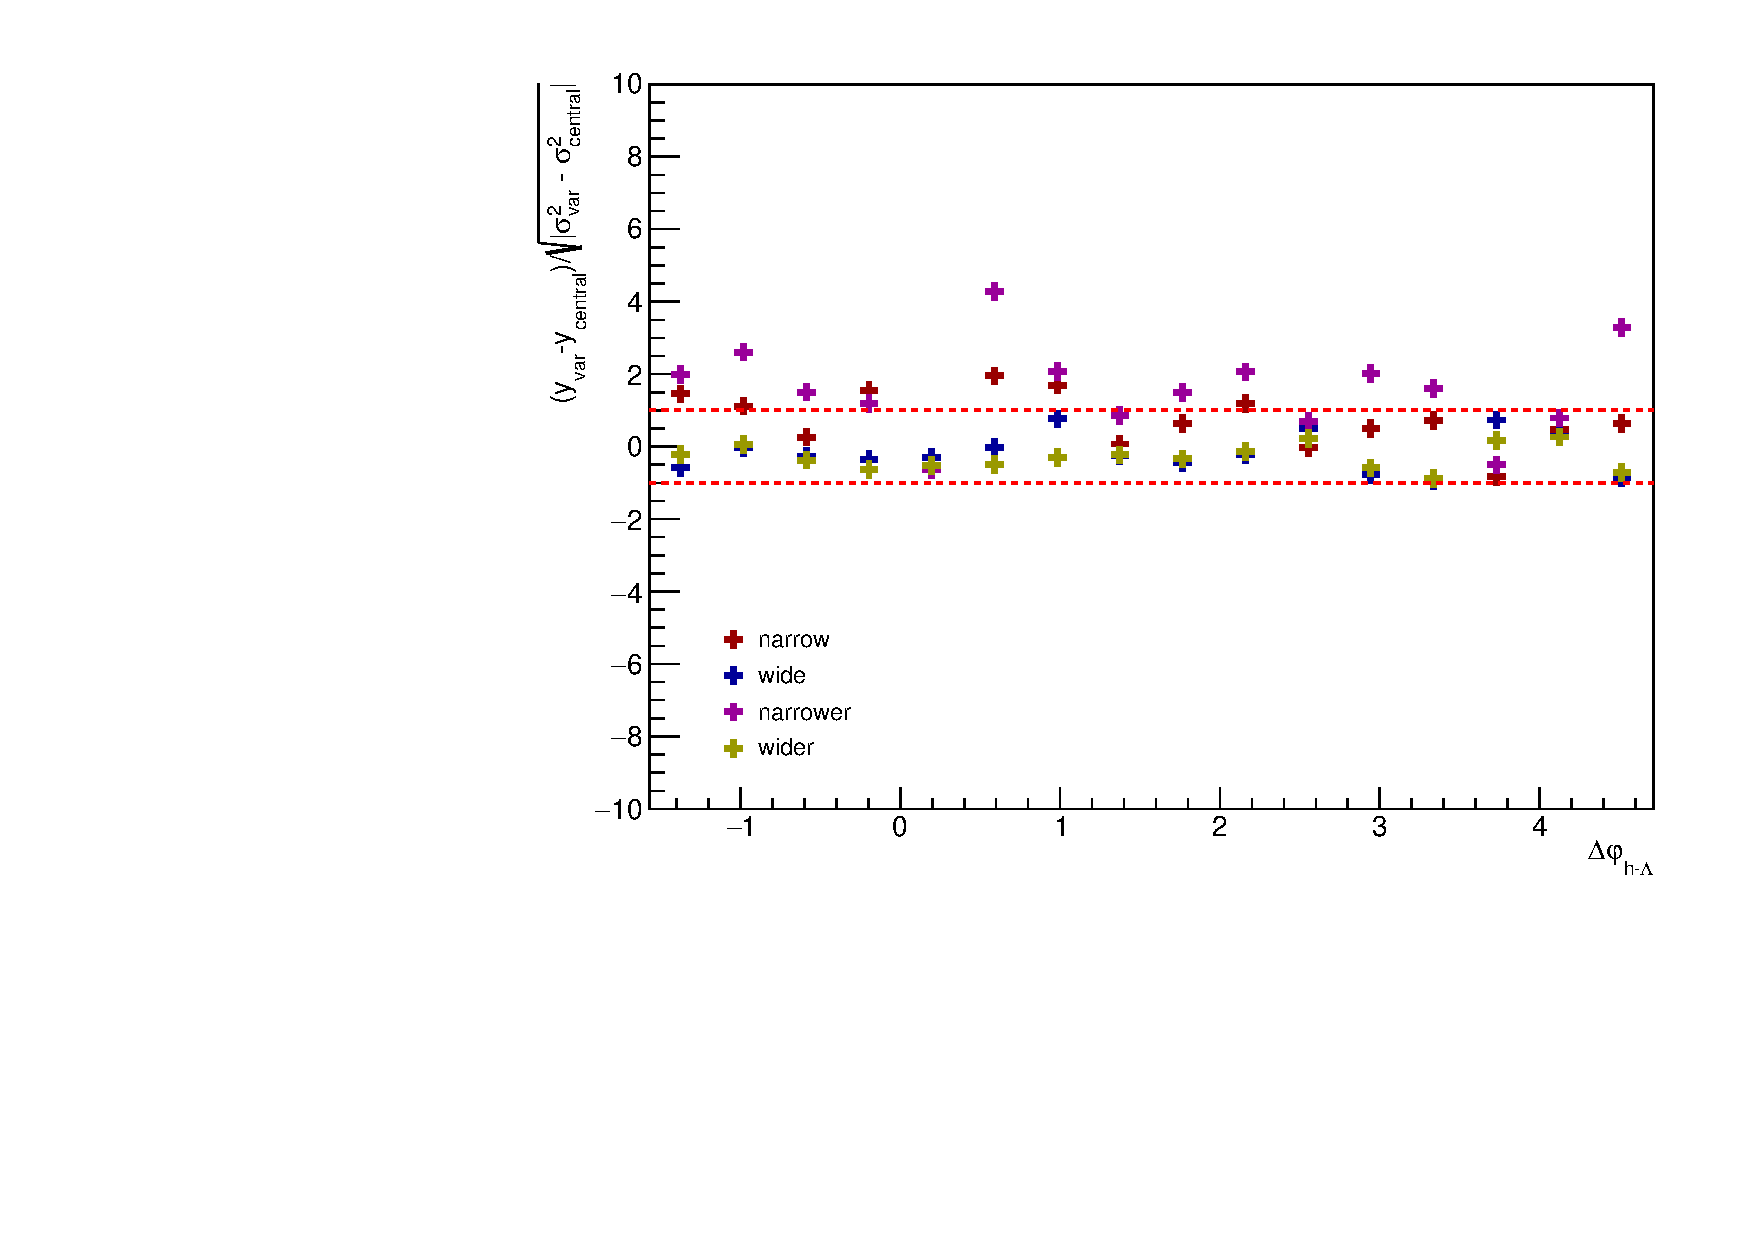
\includegraphics[width=4in]{figures/signal_barlow_0_20.pdf}}
% \end{subfigure}
% \begin{subfigure}{
% 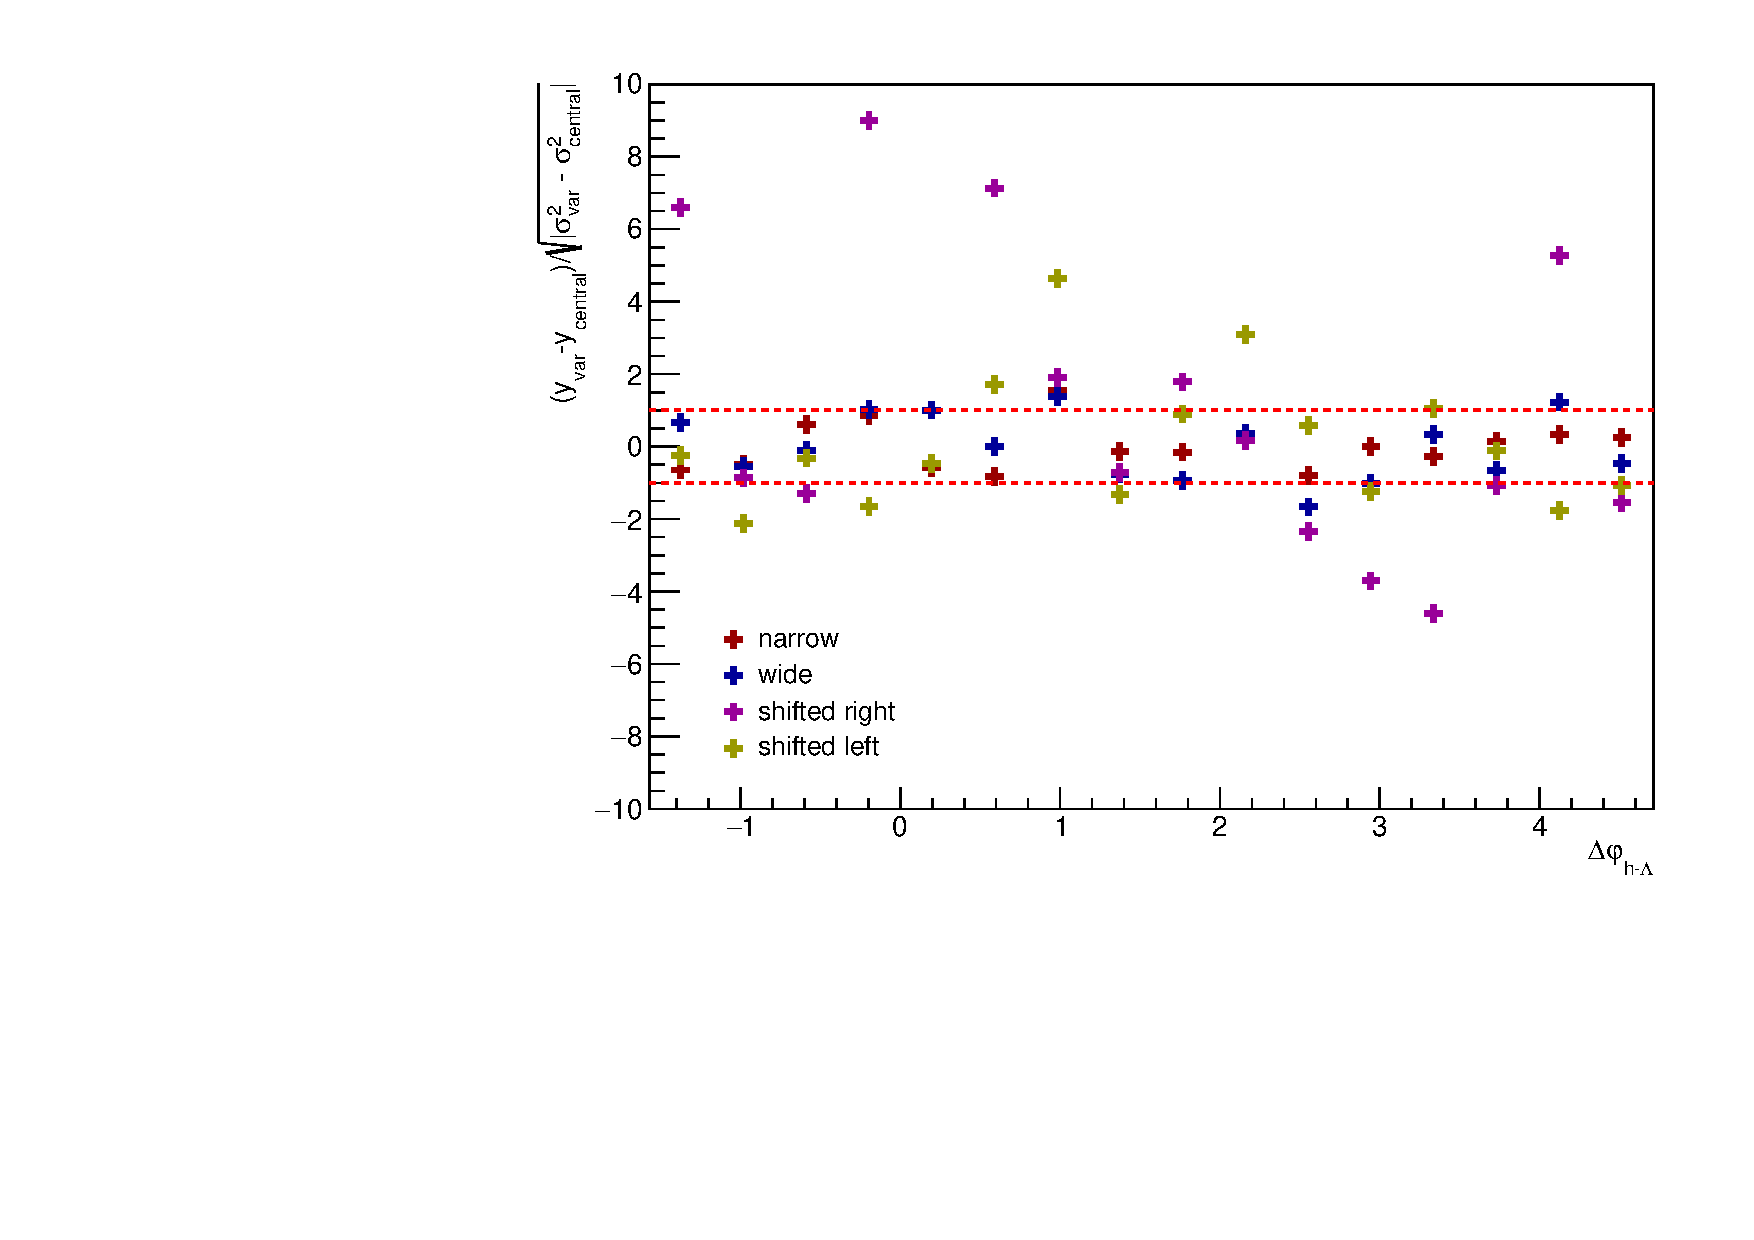
\includegraphics[width=4in]{figures/sideband_barlow_0_20.pdf}}
% \end{subfigure}
% \begin{subfigure}{
% 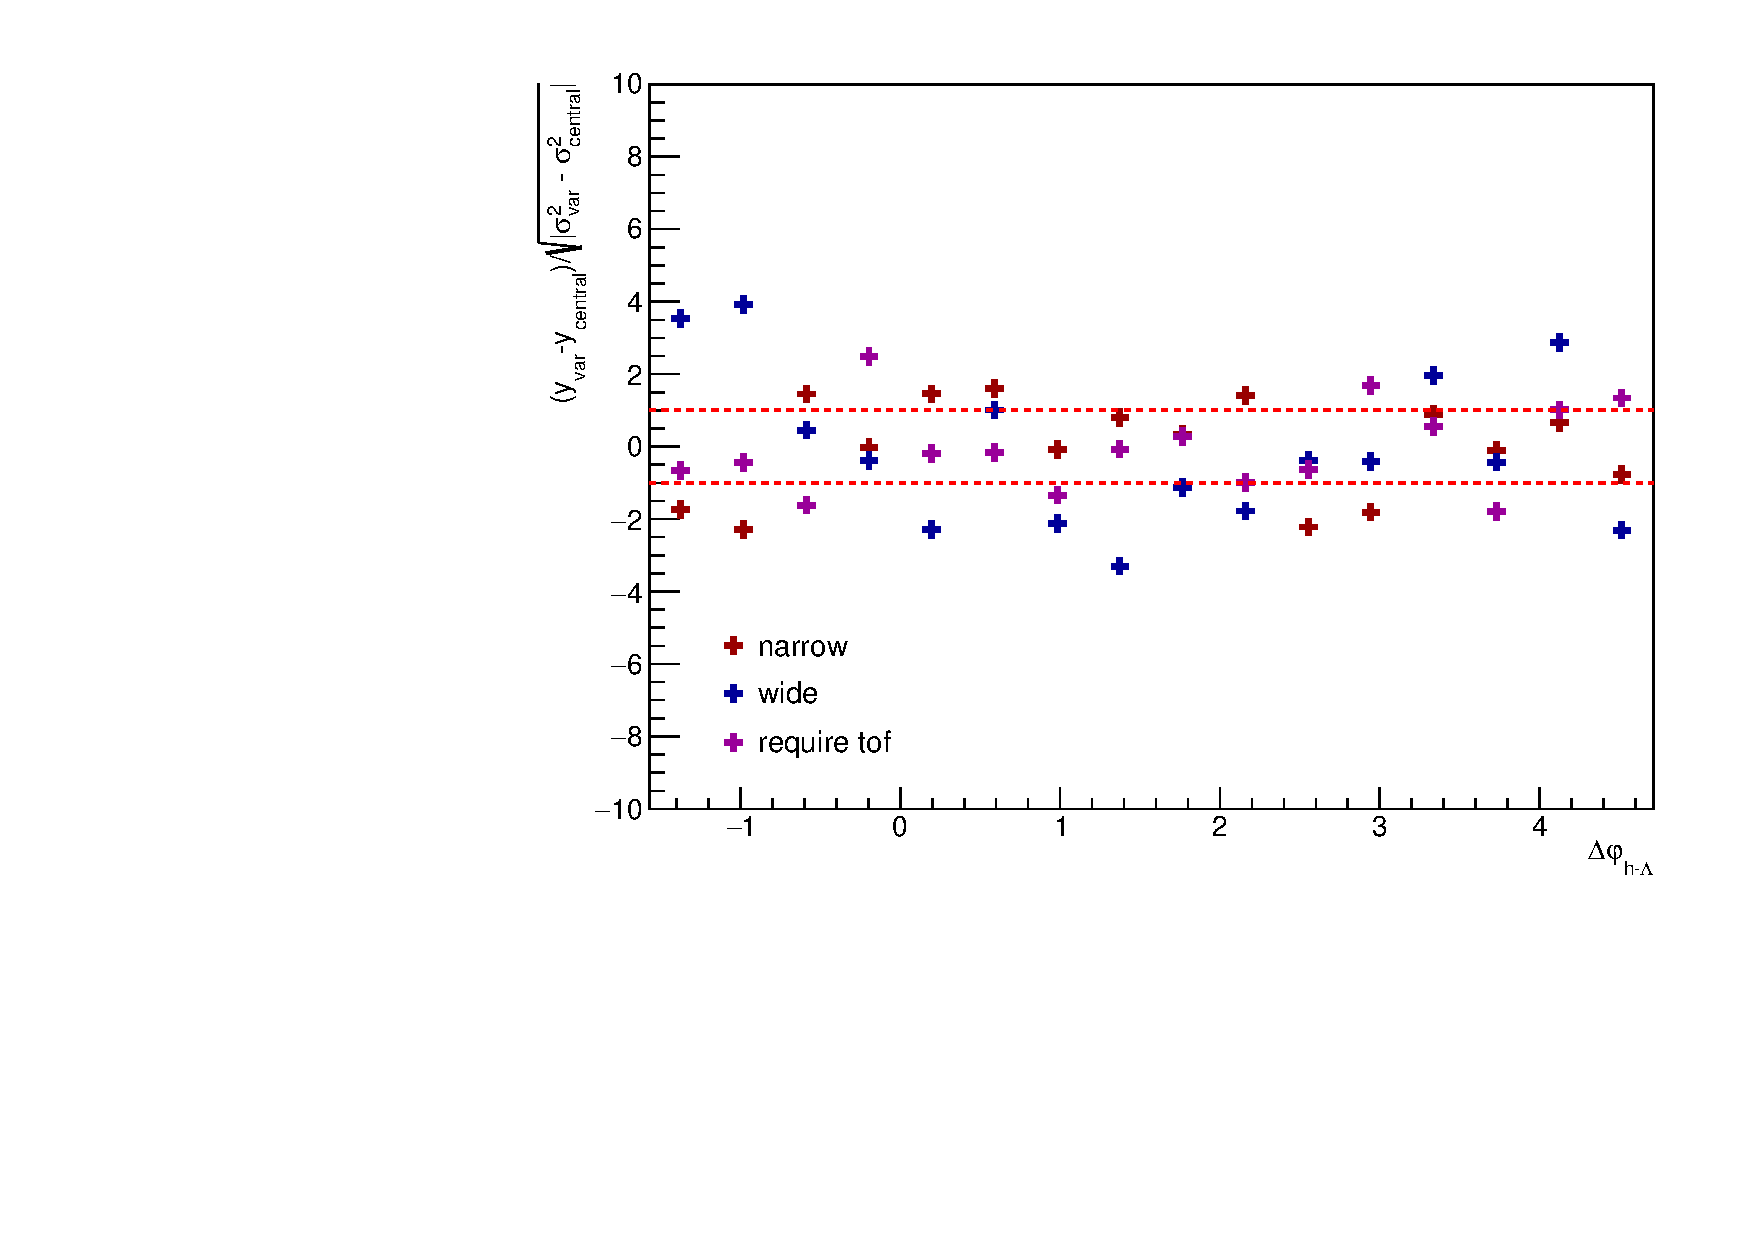
\includegraphics[width=4in]{figures/pid_barlow_0_20.pdf}}
% \end{subfigure}
% \caption{Barlow check for the signal (top), sideband (middle), and PID (bottom) variations in the 0-20\% multiplicity bin. The red lines represent $N\sigma_{RB} = \pm 1$, and if the majority of the points fall within the red lines (across all $p_{T}$ and multiplicity bins), they are excluded from the systematic uncertainty calculation.}
% \label{barlow_check_0_20}
% \end{figure}

% \clearpage

% \subsubsection{Other Sources of Systematic Uncertainty}
% \label{other_systematic_sources}
% As this analysis uses track quality cuts that have been used in previous analysis, we have assigned the following systematic errors:
% \begin{itemize}
% \item $\Lambda$ Topological Selection: 3.2\% (lower $p_{T}$), 3.0\% (central and higher $p_{T}$) (see here: \url{https://alice-notes.web.cern.ch/node/1191})
% \item $\Lambda$ Material Budget: 1.1\% (lower $p_{T}$), 0.6\% (central and higher $p_{T}$) (see here: \url{https://alice-notes.web.cern.ch/node/1191})
% \item Trigger efficiency: 3.5\% (see here: \url{https://alice-notes.web.cern.ch/node/919})
% \item Associated hadron efficiency: 3.5\% (see here: \url{https://alice-notes.web.cern.ch/node/919})
% \end{itemize}

% As it has been observed from previous analyses that the trigger tracking efficiency approximately cancels out in the final per-trigger distributions, we only consider the associated hadron and $\Lambda$ reconstruction efficiency systematic errors in our final systematic calculation for both the per-trigger $\Delta\varphi$ distributions and the final per-trigger yields.

% \subsubsection{Final Systematic Errors from $\Delta\varphi$ Distribution Generation}
% \label{final_dphi_systematics}
% A table of the final systematic errors (in percentages) from the $\Delta\varphi$ distribution generation for each multiplicity bin and $p_{T}$ bin is shown in Tables \ref{dphi_systematics_table} through \ref{dphi_systematics_table_highpt}. The total systematic is calculated by adding each systematic error in quadrature. Plots showing the systematic errors for each multiplicity bin and $p_{T}$ bin are shown in Figure \ref{dphi_systematics_plots}. We observe that the total systematic error is mostly $p_{T}$-independent. The $h-\Lambda$ and $h-h$ $\Delta\varphi$ distributions with their systematic errors are shown for our central $p_{T, assoc}$ bin in Figures \ref{h_lambda_dphi_systematics} and \ref{h_h_dphi_systematics}, respectively. The statistical errors are not shown to emphasize the systematic errors, but they are included in the final results (Section \ref{results})


% \begin{table}[ht]
% \centering
% \begin{tabular}{|c||c|c|c|c|c||c|}
% \hline
% Multiplicity Bin & Signal Region & Sideband Region & PID Cuts & Topo. Selection & Material Budget & Total \\
% \hline
% 0-20\% & 0.39 & 0.46 & 0.57 & 3.0 & 0.6 & 3.1 \\
% 20-50\% & 0.46 & 0.51 & 0.86 & 3.0  & 0.6 & 3.2 \\
% 50-80\% & 0.87 & 1.1 & 1.4 & 3.0  & 0.6 & 3.6 \\
% \hline
% \end{tabular}
% \caption{The final systematic errors from the $h-\Lambda$ $\Delta\varphi$ distribution generation for each multiplicity bin in our central $p_{T, assoc}$ bin. The $h-h$ distribution just the 3.5\% systematic from above and is thus not shown. The total systematic error is calculated by adding each systematic error in quadrature.}
% \label{dphi_systematics_table}
% \end{table}

% \begin{table}[ht]
% \centering
% \begin{tabular}{|c||c|c|c|c|c||c|}
% \hline
% Multiplicity Bin & Signal Region & Sideband Region & PID Cuts & Topo. Selection & Material Budget & Total \\
% \hline
% 0-20\% & 0.36 & 0.53 & 0.64 & 3.2 & 1.1 & 3.3 \\
% 20-50\% & 0.35 & 0.67 & 0.65 & 3.2  & 1.1 & 3.4 \\
% 50-80\% & 0.76 & 1.1 & 1.4 & 3.2  & 1.1 & 3.8 \\
% \hline
% \end{tabular}
% \caption{The final systematic errors from the $h-\Lambda$ $\Delta\varphi$ distribution generation for each multiplicity bin in our lower $p_{T, assoc}$ bin.}
% \label{dphi_systematics_table_lowpt}
% \end{table}

% \begin{table}[ht]
% \centering
% \begin{tabular}{|c||c|c|c|c|c||c|}
% \hline
% Multiplicity Bin & Signal Region & Sideband Region & PID Cuts & Topo. Selection & Material Budget & Total \\
% \hline
% 0-20\% & 0.42 & 0.42 & 0.76 & 3.0 & 0.6 & 3.2 \\
% 20-50\% & 0.4 & 0.71 & 1.2 & 3.0  & 0.6 & 3.3 \\
% 50-80\% & 1.1 & 1.6 & 2.0 & 3.0  & 0.6 & 4.1 \\
% \hline
% \end{tabular}
% \caption{The final systematic errors from the $h-\Lambda$ $\Delta\varphi$ distribution generation for each multiplicity bin in our higher $p_{T, assoc}$ bin.}
% \label{dphi_systematics_table_highpt}
% \end{table}

% \clearpage

% \begin{figure}[ht]
% \centering
% \begin{subfigure}{
% 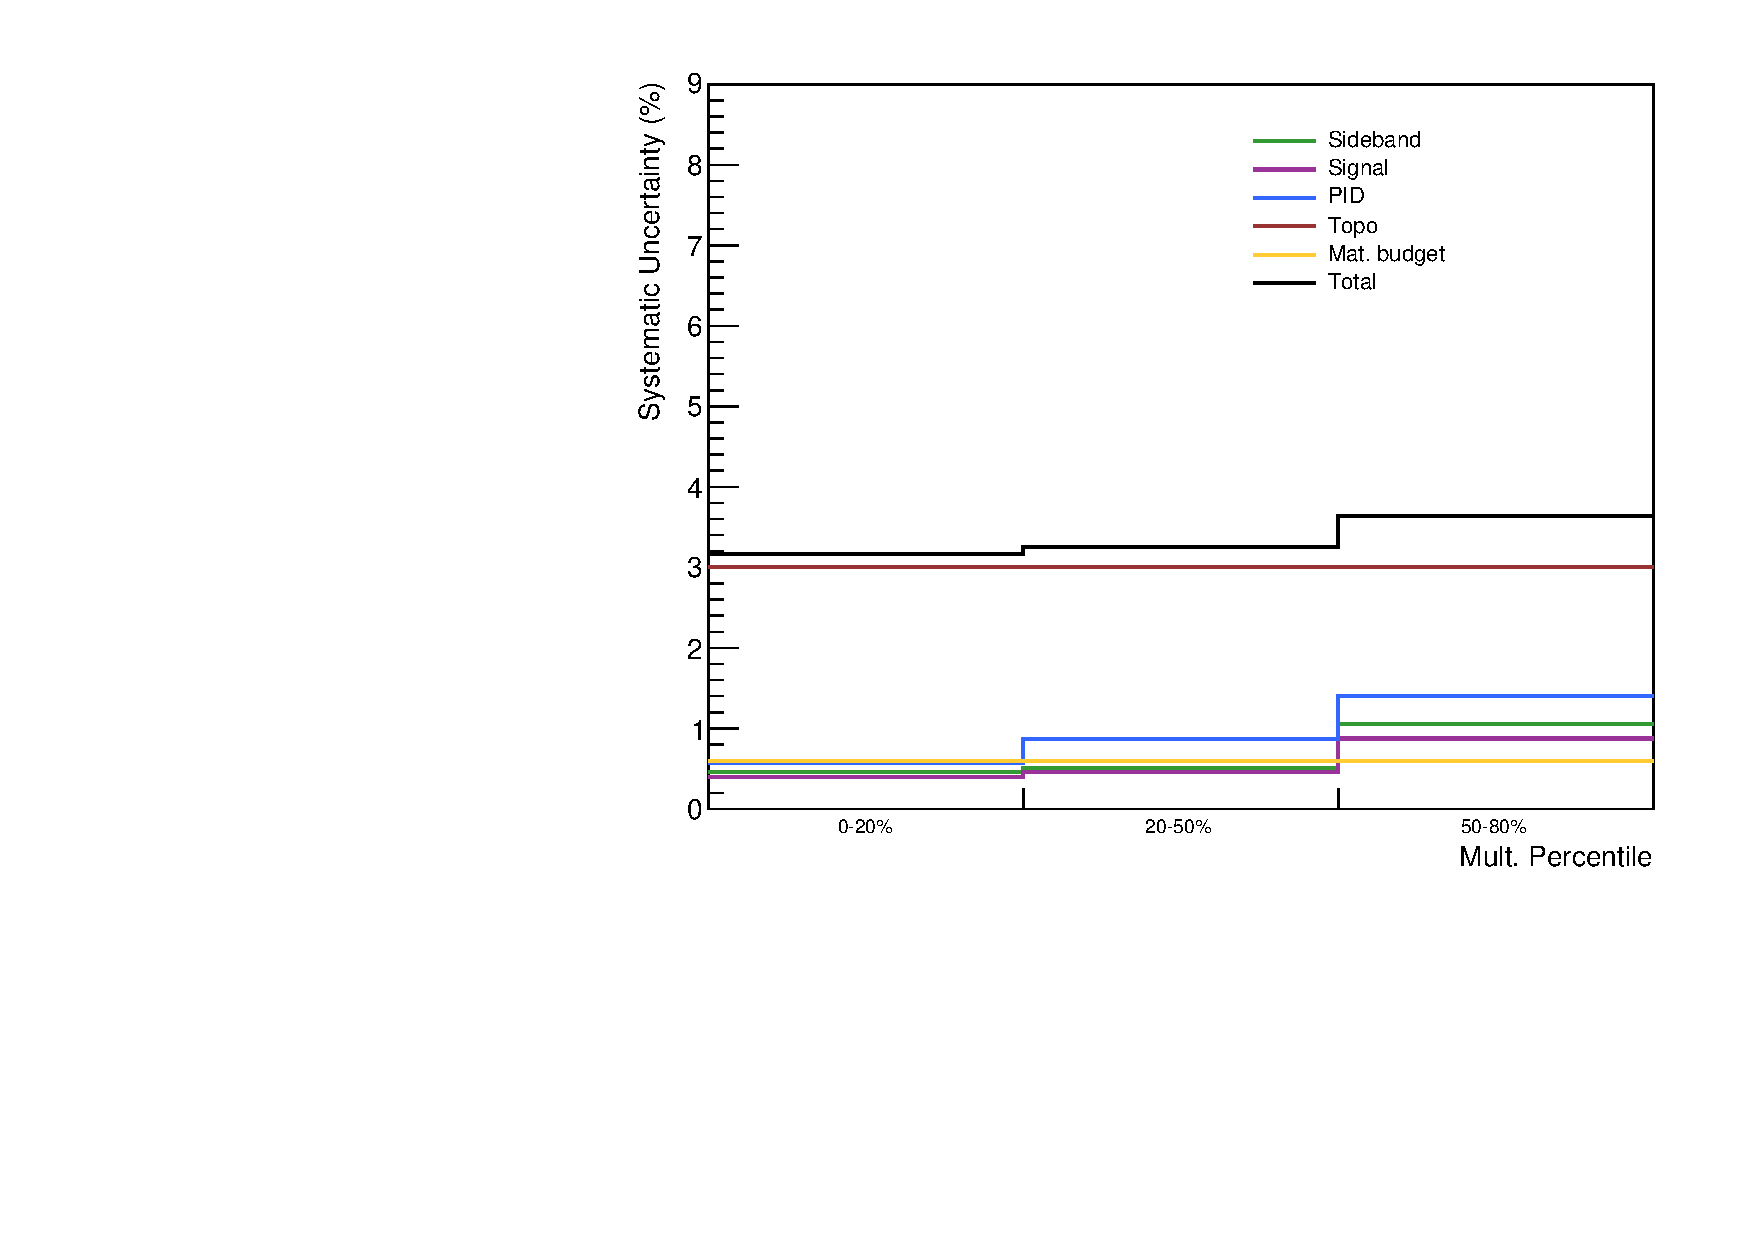
\includegraphics[width=4in]{figures/systematics_dphi_postbarlow.pdf}}
% \end{subfigure}
% \begin{subfigure}{
% 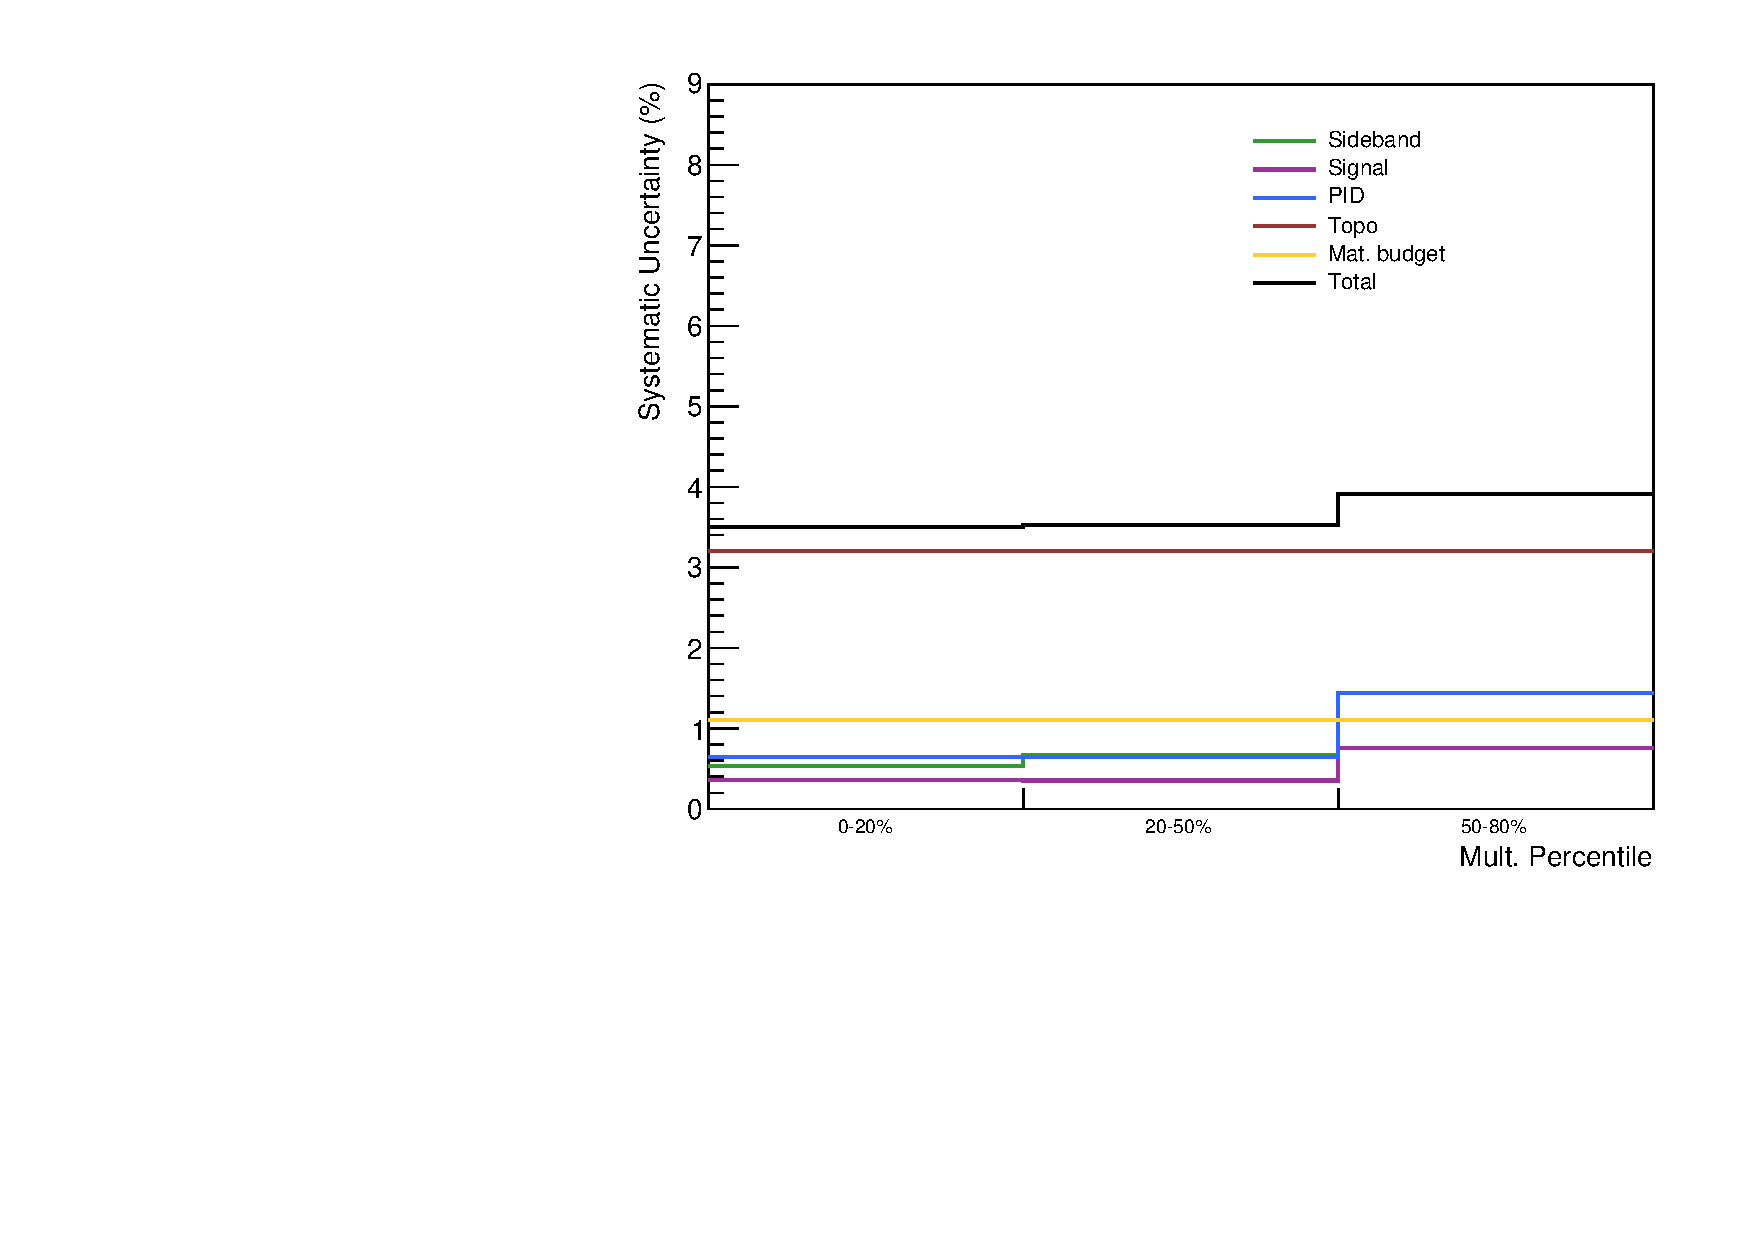
\includegraphics[width=4in]{figures/systematics_dphi_postbarlow_lowpt.pdf}}
% \end{subfigure}
% \begin{subfigure}{
% 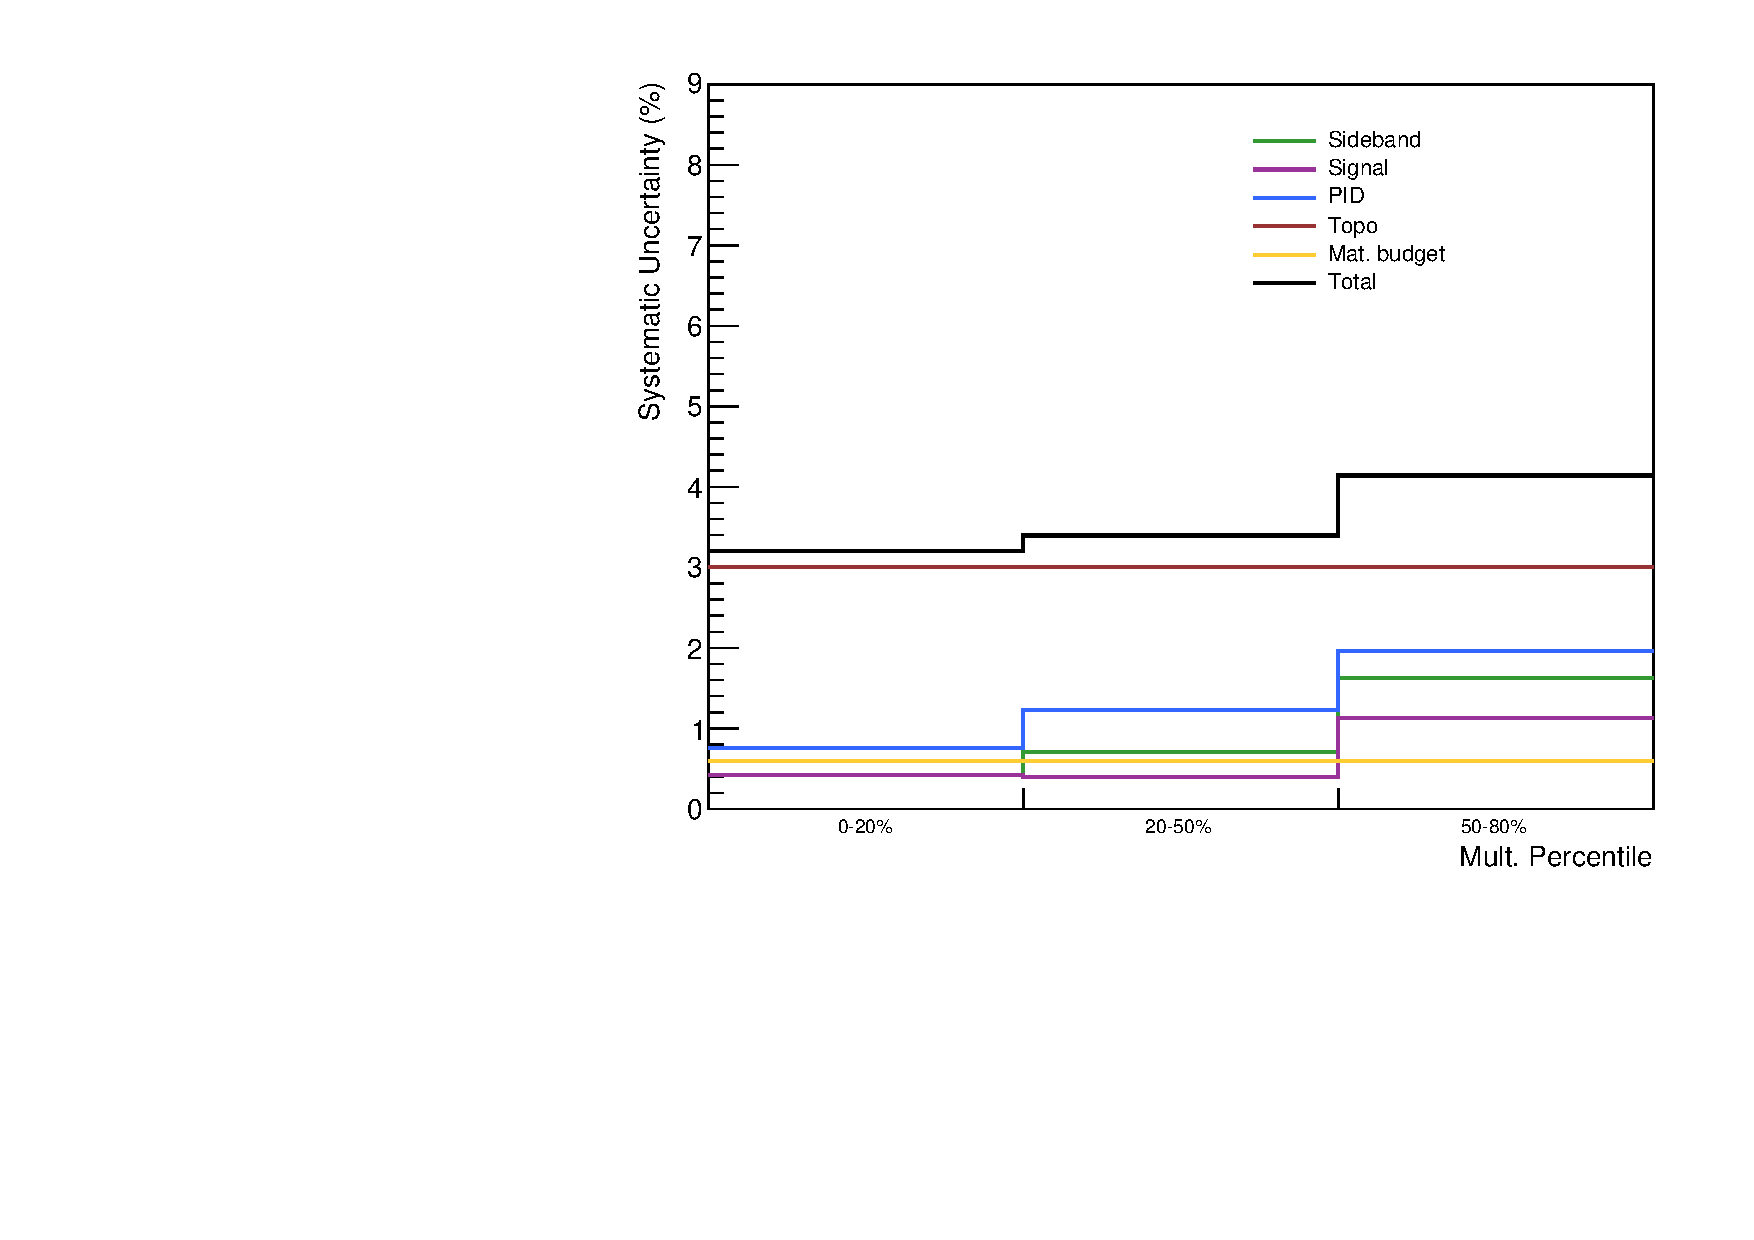
\includegraphics[width=4in]{figures/systematics_dphi_postbarlow_highpt.pdf}}
% \end{subfigure}
% \caption{Final systematic errors for the $h-\Lambda$ $\Delta\varphi$ distributions for each multiplicity bin in the central (top), lower (center) and higher (bottom) $p_{T, assoc}$ bins. We observe little-to-no dependence on $p_{T, assoc}$ for the total systematic error in each multiplicity bin.}
% \label{dphi_systematics_plots}
% \end{figure}

% \clearpage

% \begin{figure}[ht]
% \centering
% \begin{subfigure}{
% 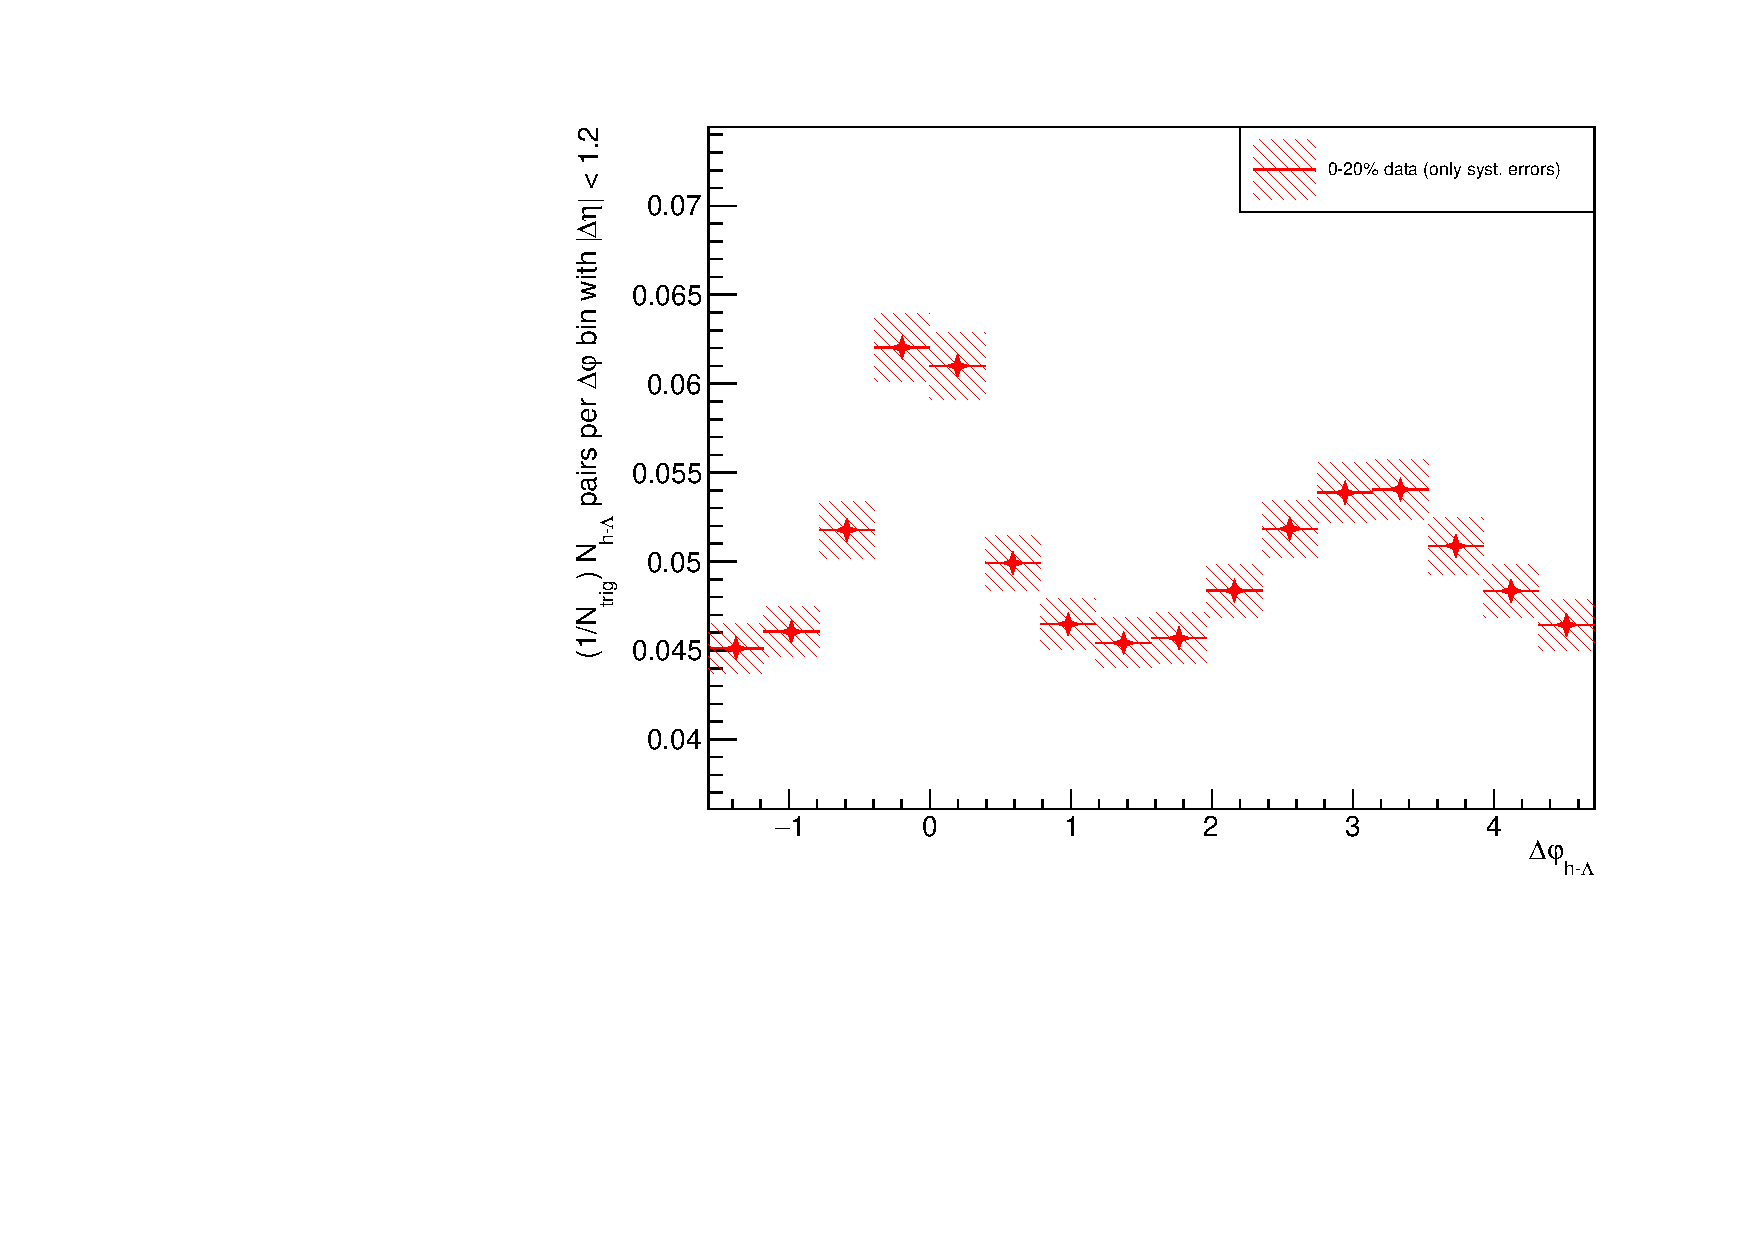
\includegraphics[width=4in]{figures/h_lambda_dphi_0_20_onlysyst.pdf}}
% \end{subfigure}
% \begin{subfigure}{
% 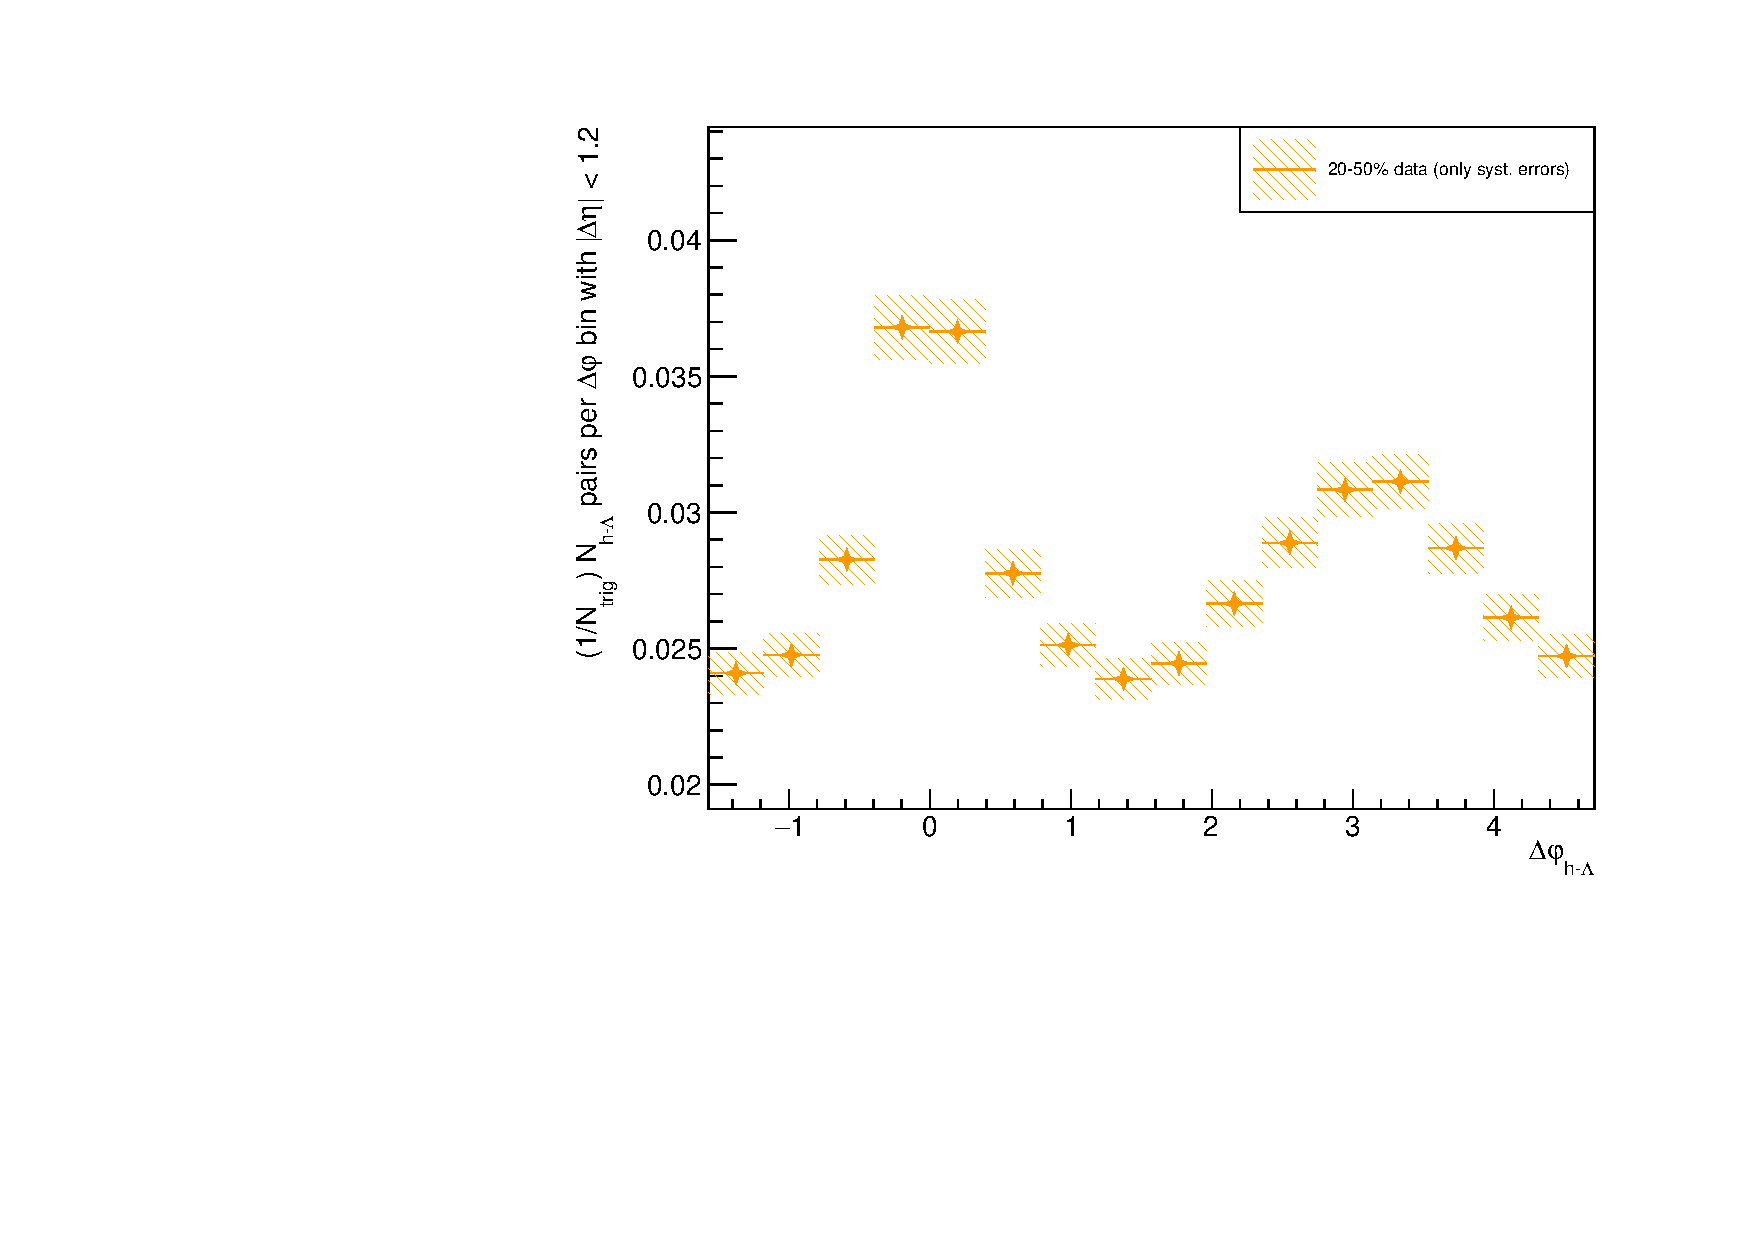
\includegraphics[width=4in]{figures/h_lambda_dphi_20_50_onlysyst.pdf}}
% \end{subfigure}
% \begin{subfigure}{
% 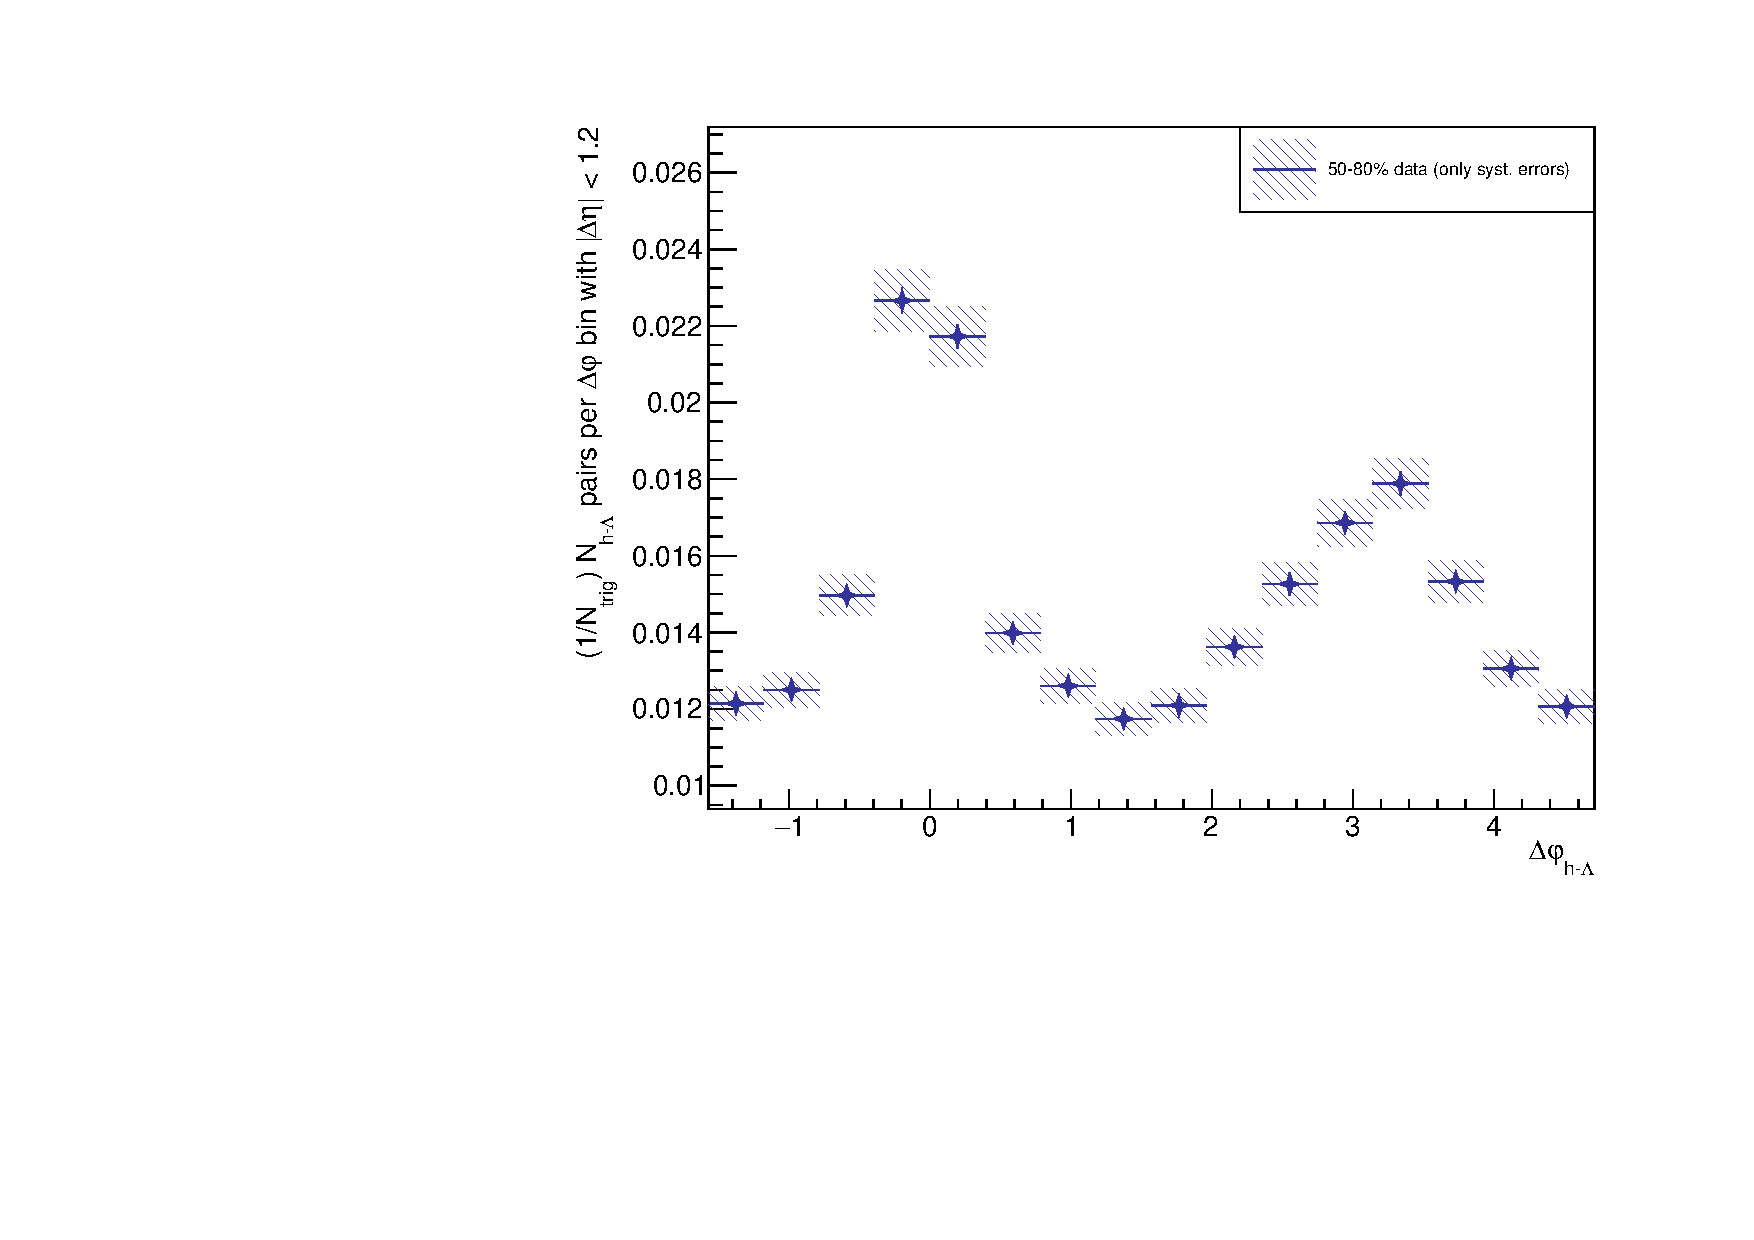
\includegraphics[width=4in]{figures/h_lambda_dphi_50_80_onlysyst.pdf}}
% \end{subfigure}
% \caption{Per-trigger normalized $\Delta\varphi$ correlations for h-$\Lambda$ pairs in the 0-20\% (top), 20-50\% (center) and 50-80\% (bottom) multiplicity bins in our central $p_{T, assoc}$ bin with the systematic errors shown for each bin (statistical errors are not shown).}
% \label{h_lambda_dphi_systematics}
% \end{figure}

% \begin{figure}[ht]
% \centering
% \begin{subfigure}{
% 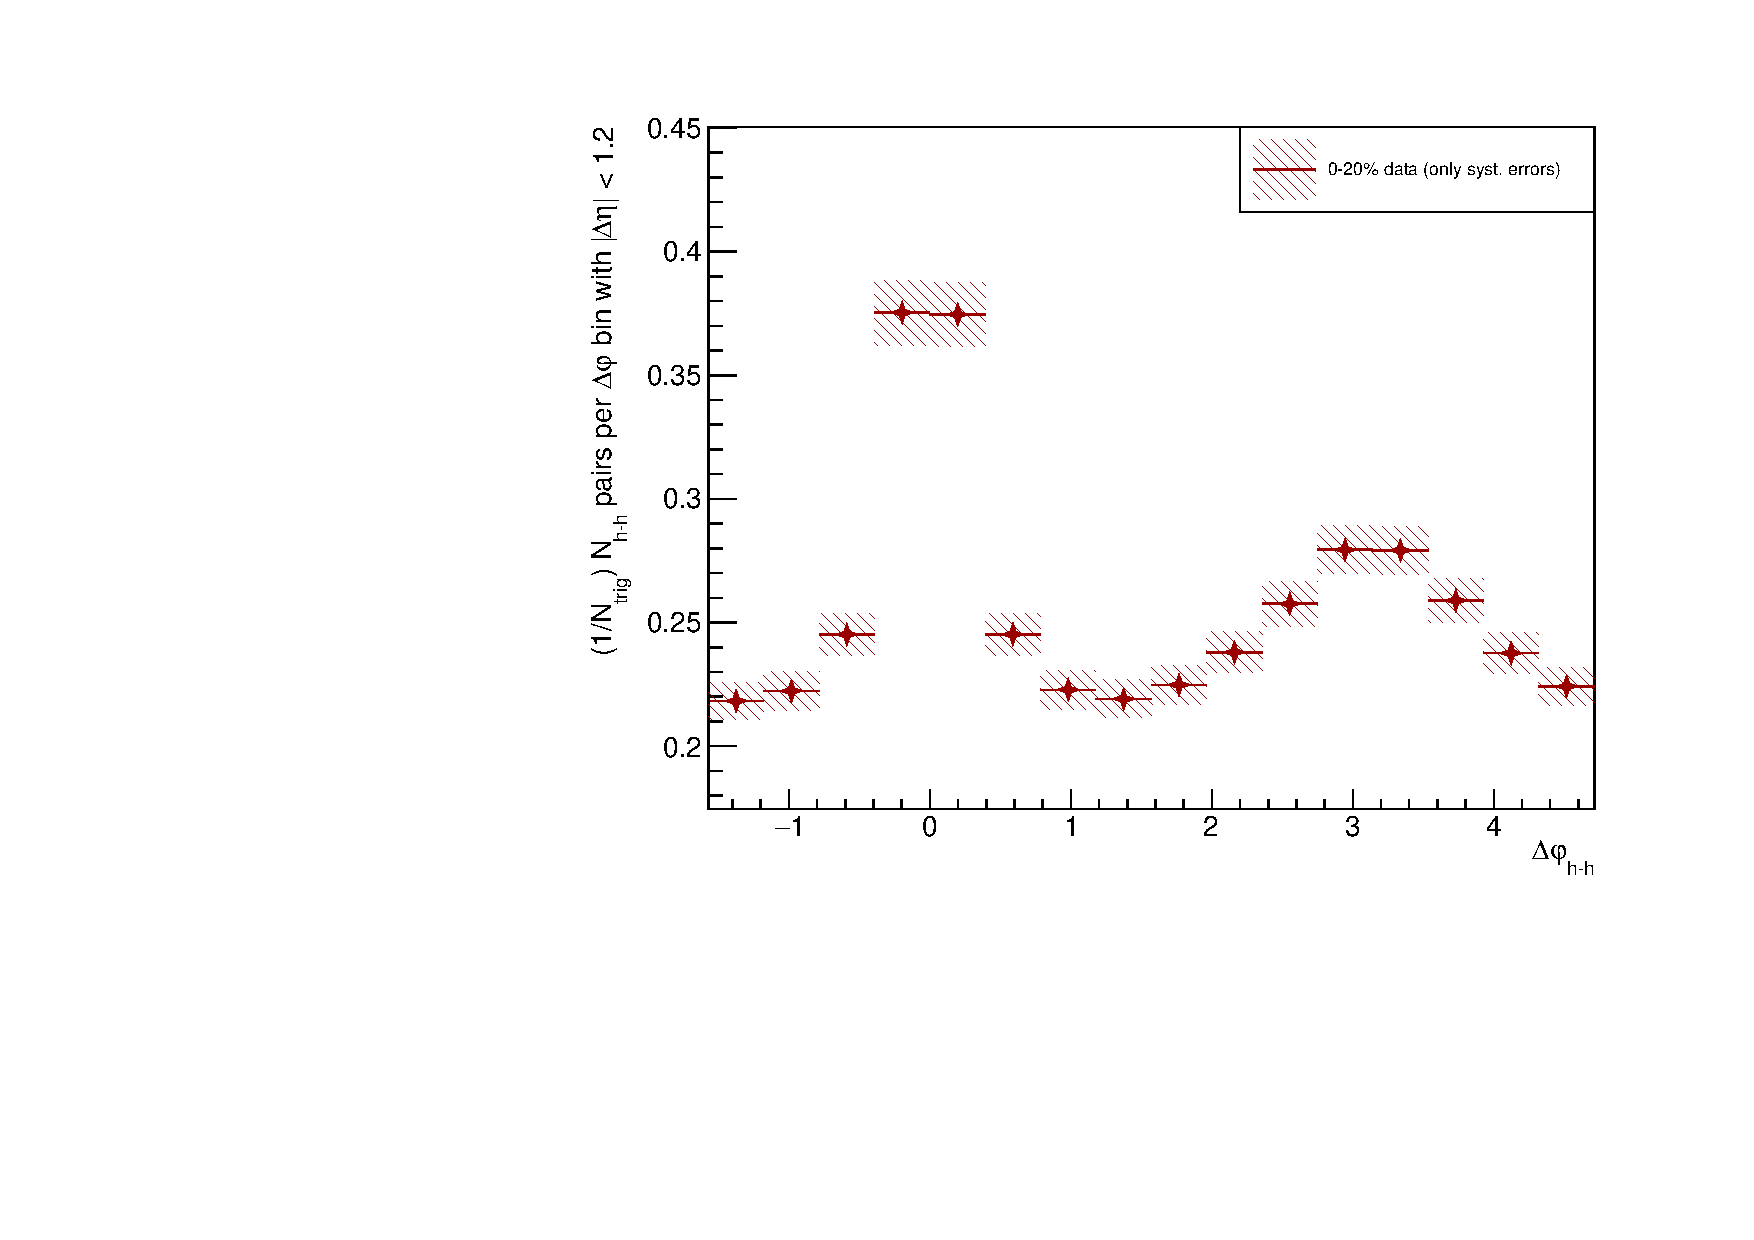
\includegraphics[width=4in]{figures/h_h_dphi_0_20_onlysyst.pdf}}
% \end{subfigure}
% \begin{subfigure}{
% 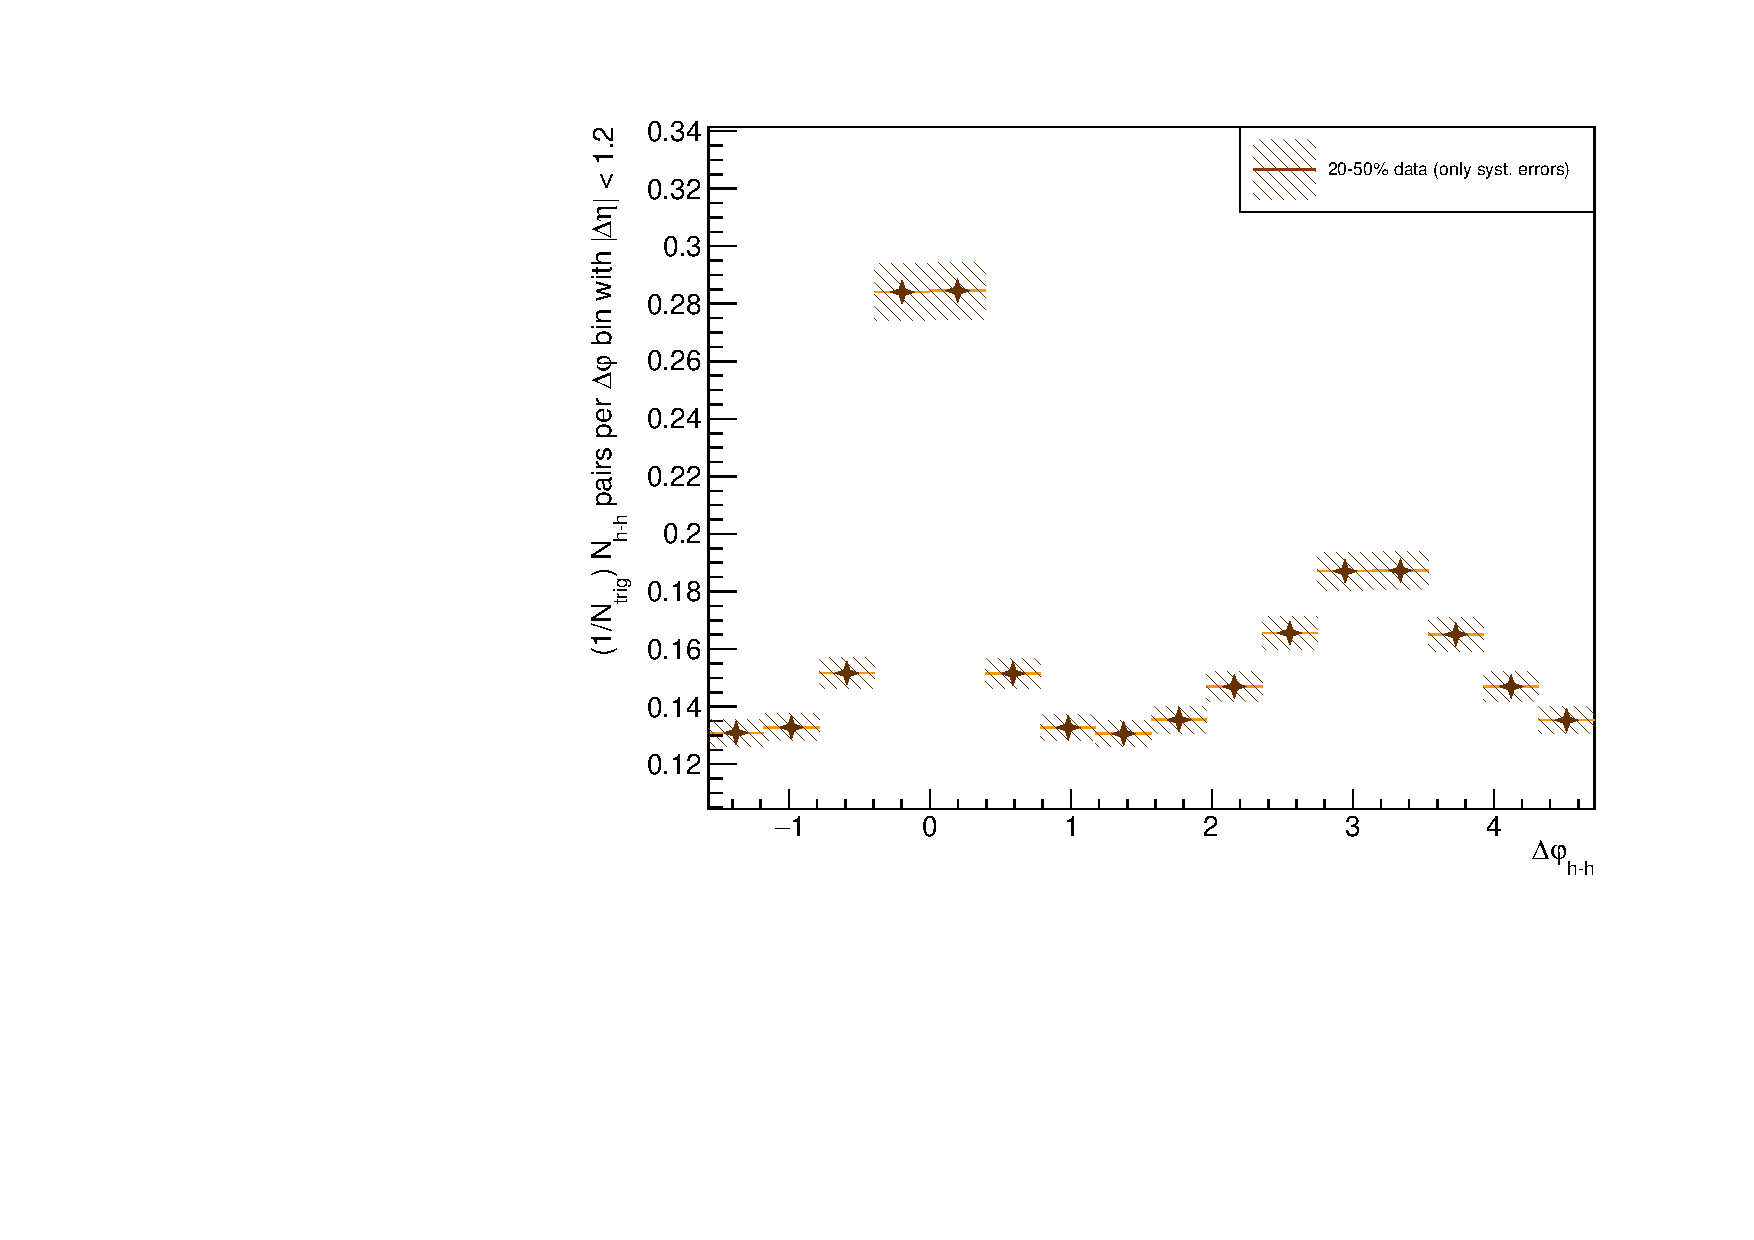
\includegraphics[width=4in]{figures/h_h_dphi_20_50_onlysyst.pdf}}
% \end{subfigure}
% \begin{subfigure}{
% 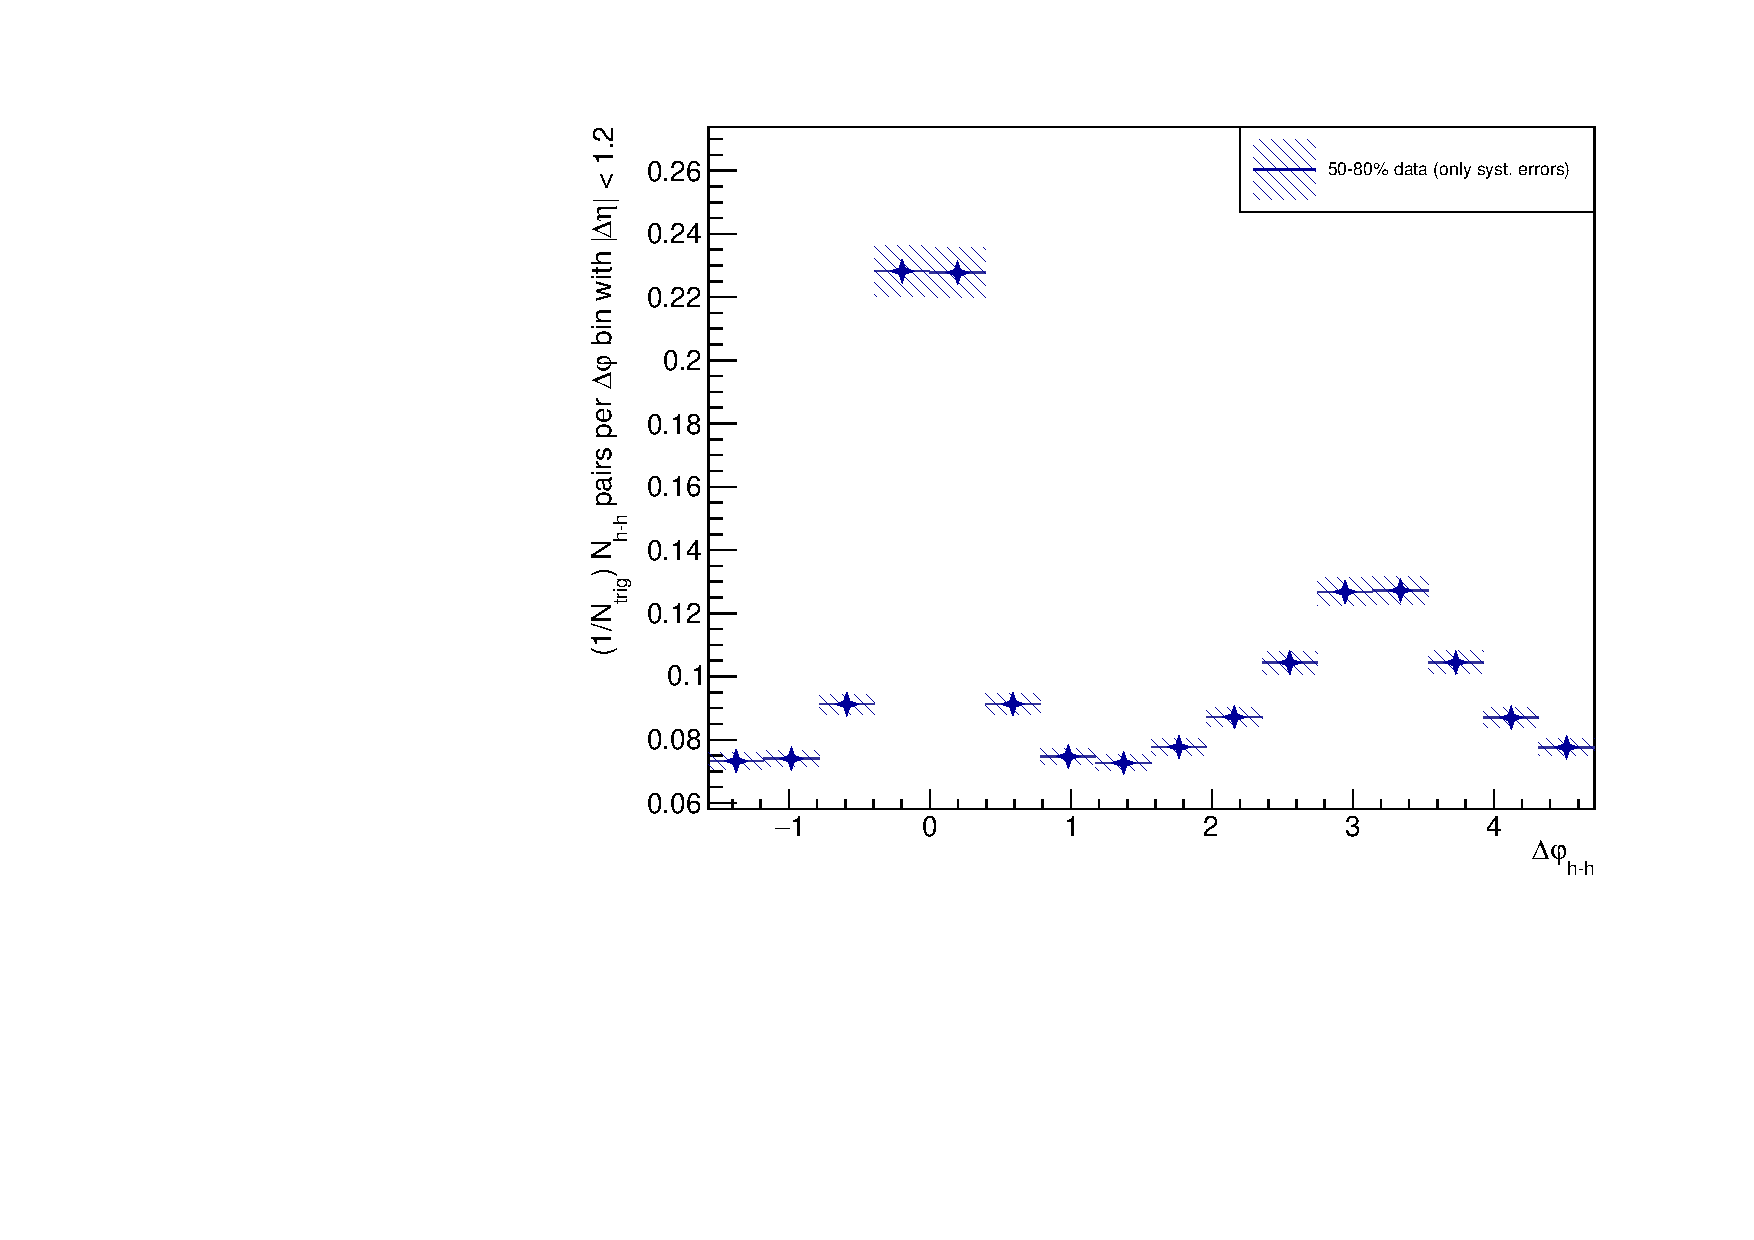
\includegraphics[width=4in]{figures/h_h_dphi_50_80_onlysyst.pdf}}
% \end{subfigure}
% \caption{Per-trigger normalized $\Delta\varphi$ correlations for h-h pairs in the 0-20\% (top), 20-50\% (center) and 50-80\% (bottom) multiplicity bins in our central $p_{T, assoc}$ bin with the systematic errors shown for each bin (statistical errors are not shown).}
% \label{h_h_dphi_systematics}
% \end{figure}

% \clearpage

% \subsubsection{$N_{ch}$-Dependent Systematics (for $\Delta\varphi$ distributions)}

% \label{nch_dep_systematics_dphi}
% In some of the results for this analysis, we take straight-line (pol1) fits of points vs. $<\frac{dN_{ch}}{d\eta}>$. Such fits should only be taken considering the fraction of systematic uncertainty that is uncorrelated with multiplicity ($N_{ch}$-dependent). Because of this, we approximate this multiplicity-uncorrelated fraction using the following formula:
% \begin{equation}
% \sigma_{uncor, i}^2 = \sum_{var}(R_{var, i} - 1)^2,
% \end{equation}
% where 
% \begin{equation}
% R_{var, i} = \frac{y_{var, i}}{y_{central, i}}/ \frac{y_{var}^{MB}}{y_{central}^{MB}},
% \end{equation}
% where ``i'' refers to the ith multiplicity bin, and ``MB'' refers to the min-bias (multiplicity-integrated) results. We compute $\sigma_{uncor, i}$ in each $\Delta\varphi$ bin, then take the RMS across all $\Delta\varphi$ bins (as there is no $\Delta\varphi$ dependence) to obtain the final multiplicity-uncorrelated portion of our systematic errors. The results for each $p_{T, assoc}$ bin are shown in Figure \ref{dphi_nch_dep_systematics_plots}.

% \clearpage

% \begin{figure}[ht]
% \centering
% \begin{subfigure}{
% 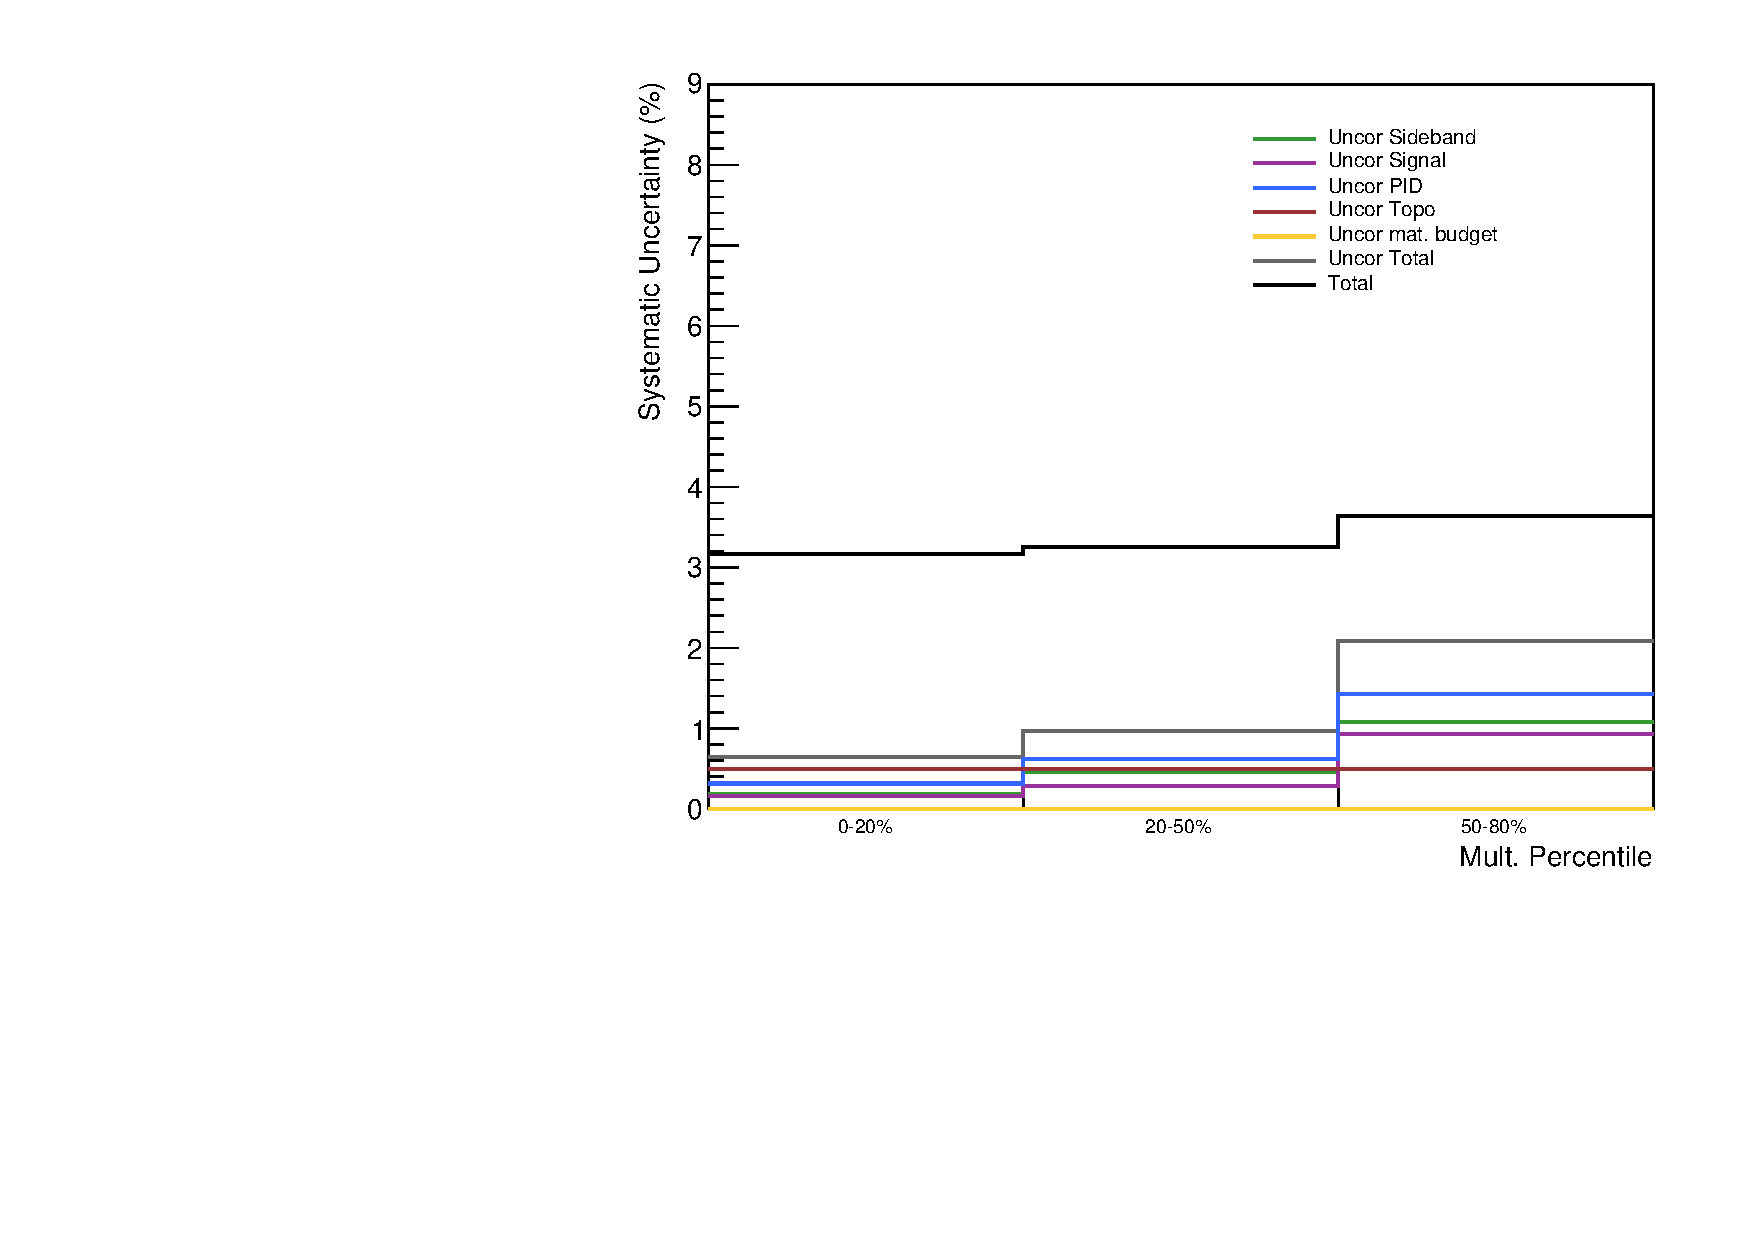
\includegraphics[width=4in]{figures/nch_dep_systematics_dphi_postbarlow.pdf}}
% \end{subfigure}
% \begin{subfigure}{
% 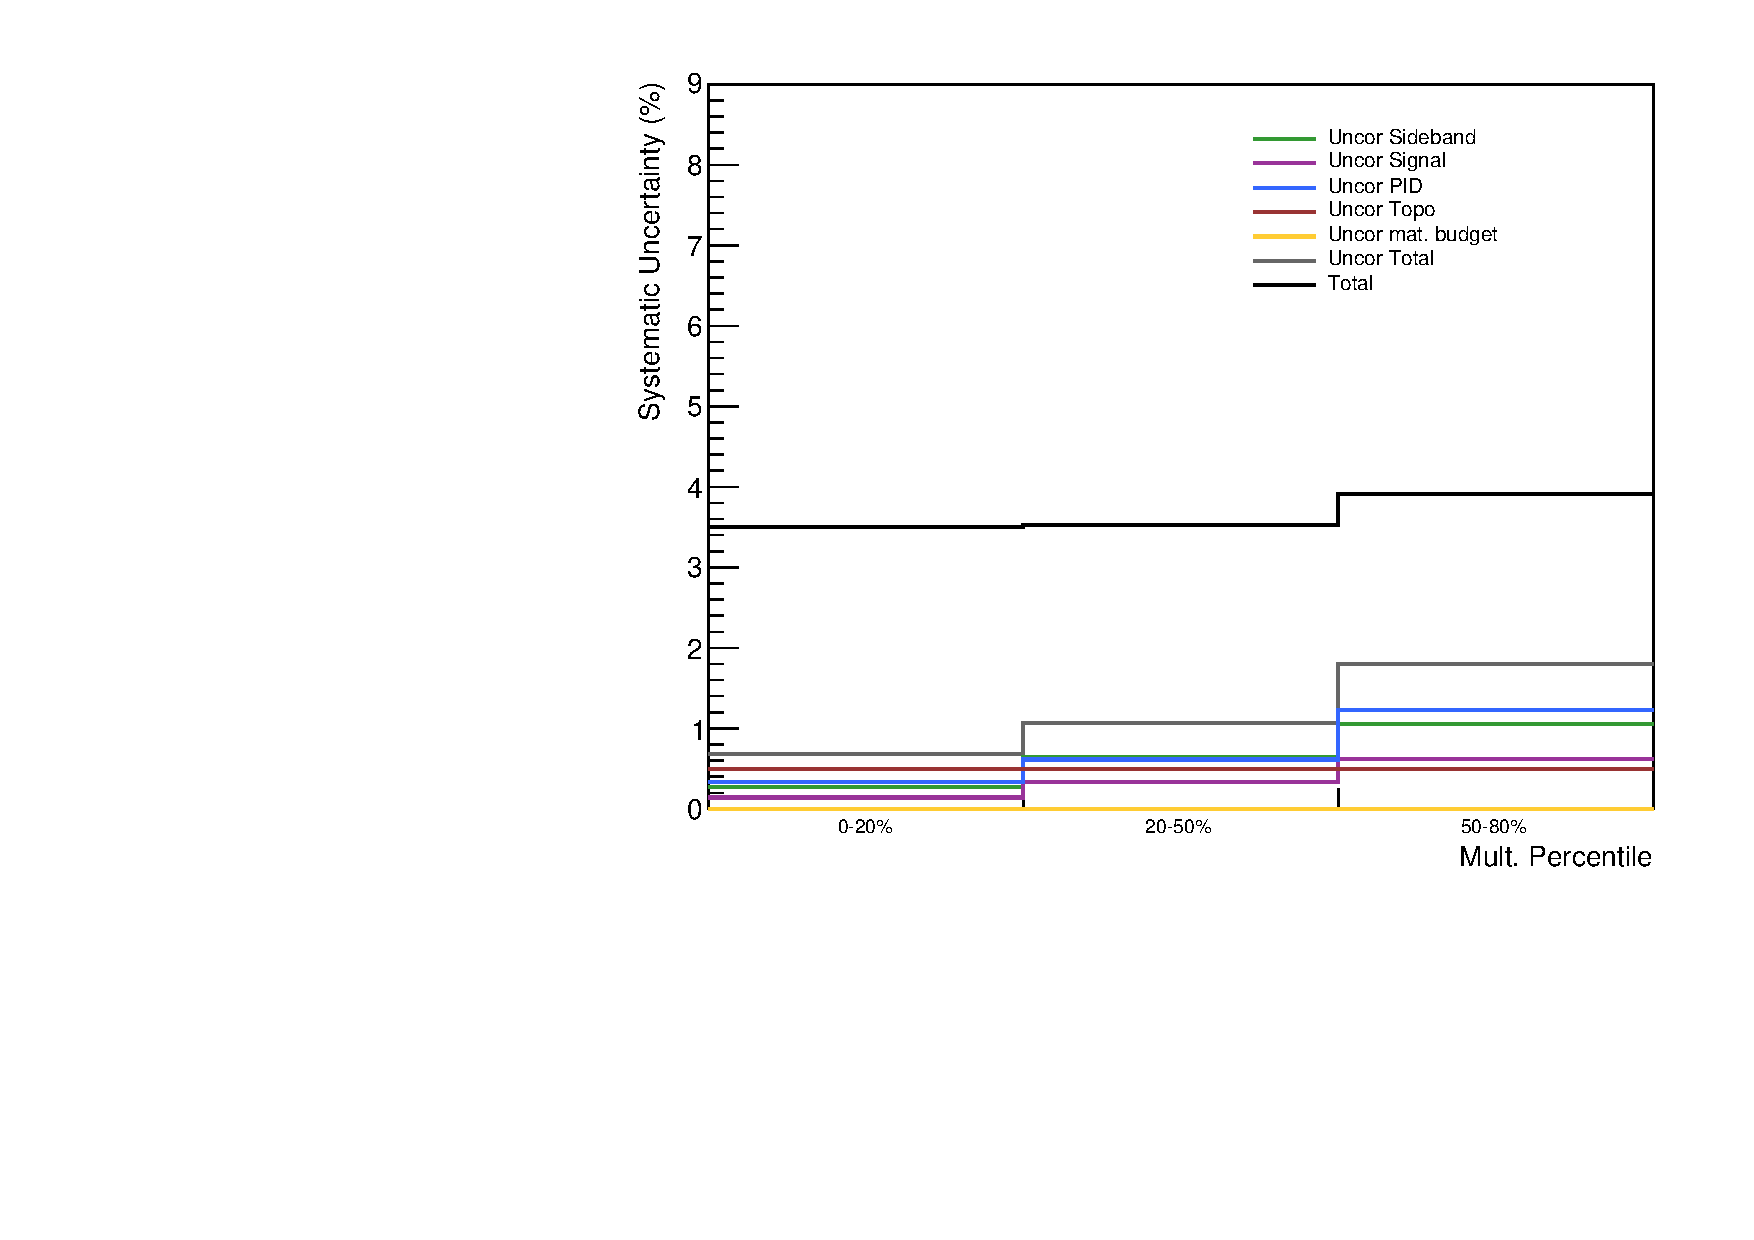
\includegraphics[width=4in]{figures/nch_dep_systematics_dphi_postbarlow_lowpt.pdf}}
% \end{subfigure}
% \begin{subfigure}{
% 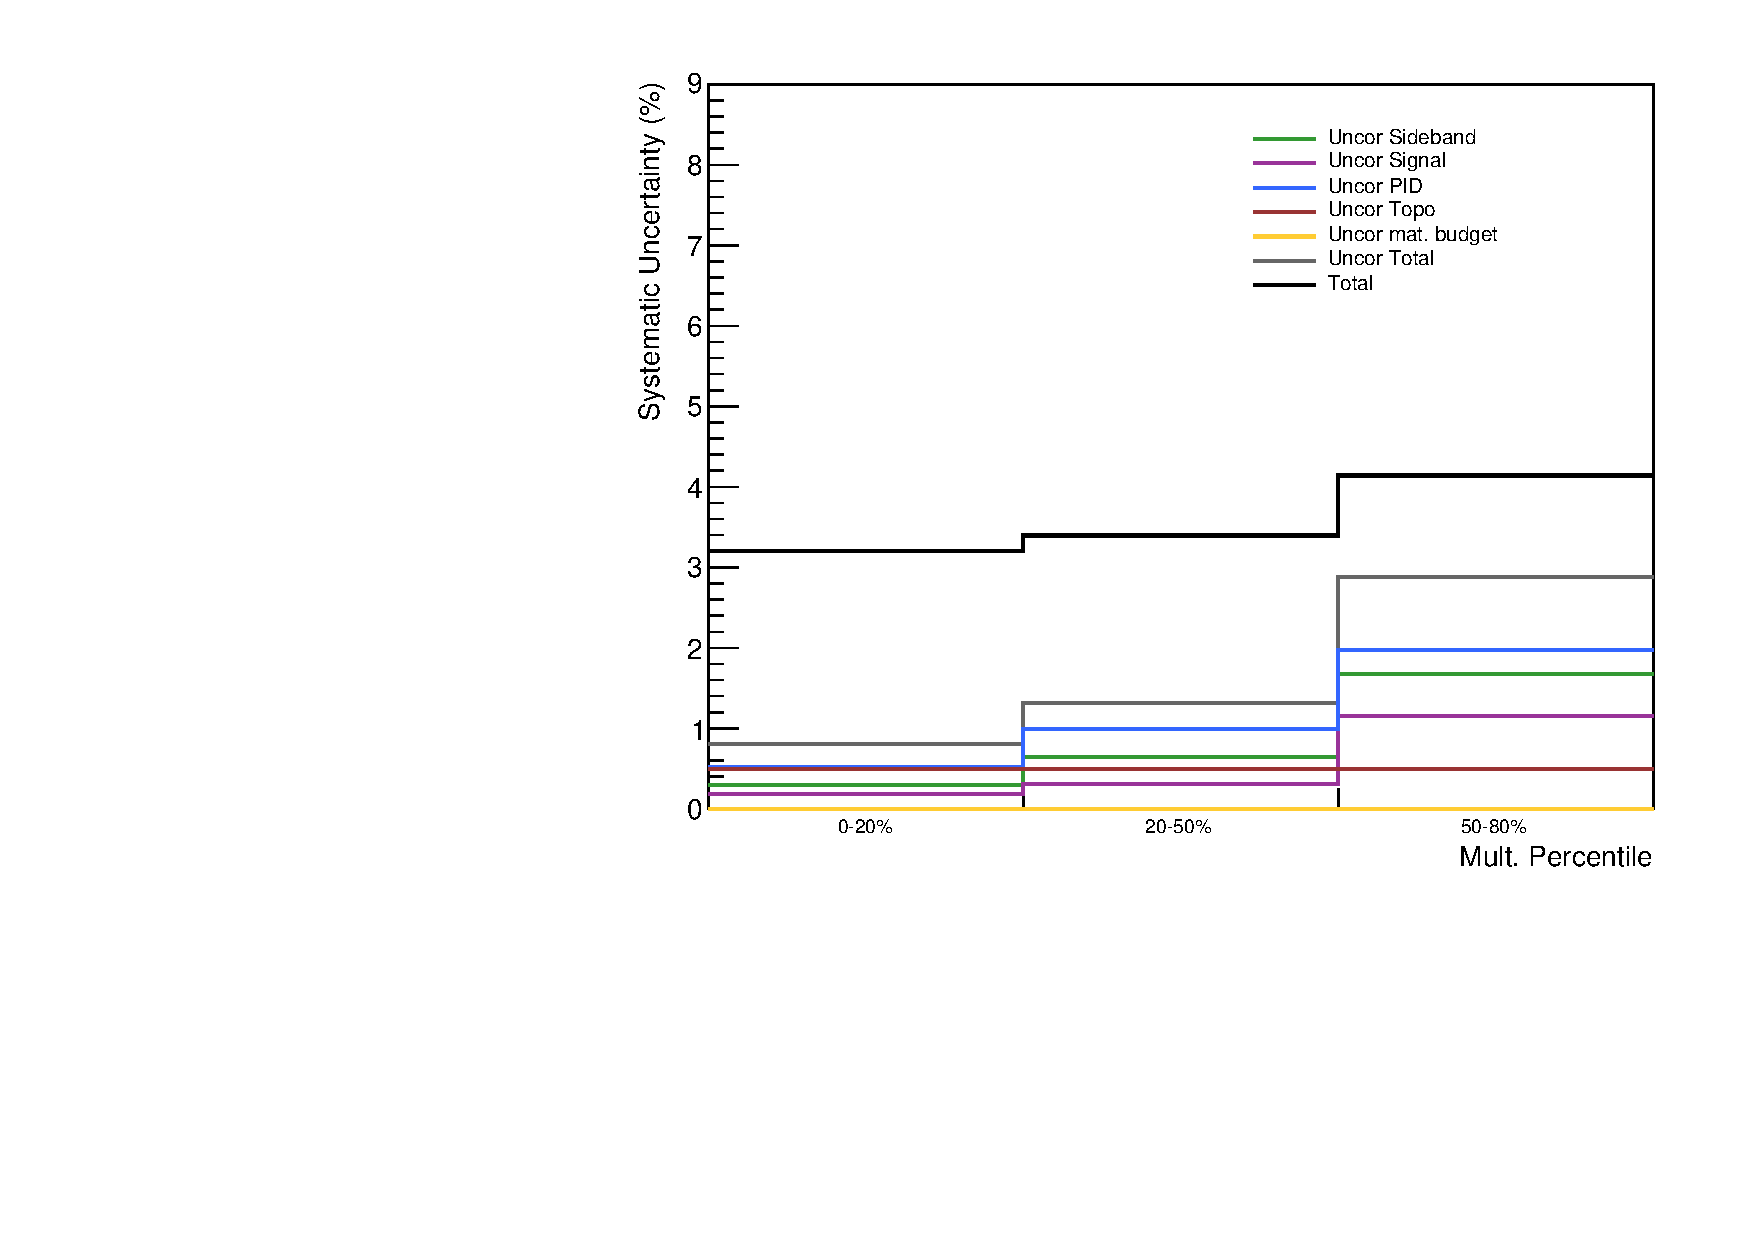
\includegraphics[width=4in]{figures/nch_dep_systematics_dphi_postbarlow_highpt.pdf}}
% \end{subfigure}
% \caption{Final multiplicity-uncorrelated systematic errors for the $h-\Lambda$ $\Delta\varphi$ distributions for each multiplicity bin in the central (top), lower (center) and higher (bottom) $p_{T, assoc}$ bins, along with the total systematic error shown in black.}
% \label{dphi_nch_dep_systematics_plots}
% \end{figure}

% \clearpage



% \subsection{Yield Extraction}
% The largest source of systematic uncertainty of this analysis corresponds to the different techniques that can be used to extract the yields in each kinematic region from the $\Delta\varphi$ distributions. We have already discussed the \textbf{6-bin underlying event technique} in Section \ref{yield_extraction}, but we will also consider the following methods. We present only the tables and plots for each technique in our central $p_{T, assoc}$ bin, but the extraction procedures are indentical for each $p_{T, assoc}$ bin.

% \subsubsection{4-bin Underlying Event Technique}
% \label{4bin}
% The 4-bin UE technique is very similar to the 6-bin UE technique, but we only select 4 bins to get an average for our UE baseline. The technique is as follows:

% \begin{itemize}
% \item The underlying event region is defined using a straight-line fit of the average of bins (1, 8, 9, 16) in the $\Delta\varphi$ distribution
% \item The near-side yield is calculated via $\sum_{i=1}^{8} (\Delta\varphi_\text{bin i} - \text{UE}_i)$, where $\text{UE}_i$ is the value of the straight-line fit at the center of the ith bin
% \item The away-side yield is calculated via $\sum_{i=9}^{16} (\Delta\varphi_\text{bin i} - \text{UE}_i)$, where $\text{UE}_i$ is the value of the straight-line fit at the center of the ith bin
% \item The underlying-event yield is calculated via $\sum_{i=1}^{16} \text{UE}_i = 16 \times UE$
% \item The total-yield is calculated via $\sum_{i=1}^{16} \Delta\varphi_\text{bin i} = \text{near-side} + \text{away-side} + \text{underlying-event}$
% \end{itemize}

% The final per-trigger $\Delta\varphi$ plots with the UE fit using the 4-bin UE technique are shown in Figures \ref{h_lambda_dphi_uefit_4bin} ($h-\Lambda$) and \ref{h_h_dphi_uefit_4bin} ($h-h$), and the extracted yields are shown in Table \ref{h_lambda_yield_table_4bin} ($h-\Lambda$) and Table \ref{h_h_yield_table_4bin} ($h-h$).

% \begin{table}[h!]
% \centering
% \begin{tabular}{| c || c | c | c | c | }
% \hline
% Multiplicity Bin & Near-side Jet & Away-side Jet & Underlying Event & Total  \\
% \hline

% 0-20\% & 4.25e-02  & 3.41e-02  & 7.31e-01 & 8.07e-01 \\
% 20-50\% & 3.30e-02 & 2.72e-02  & 3.89e-01 & 4.49e-01 \\
% 50-80\% & 2.62e-02 & 2.01e-02  & 1.92e-01 & 2.39e-01 \\

% \hline
% \end{tabular}
% \caption{Per-trigger pairwise $h-\Lambda$ extracted yields and corresponding statistical errors in the different kinematic regions for each multiplicity bin. The yields were extracted using the 4-bin technique described in this section.}
% \label{h_lambda_yield_table_4bin}
% \end{table}
	
% \begin{table}[h!]
% \centering
% \begin{tabular}{| c || c | c | c | c | }
% \hline
% Multiplicity Bin & Near-side Jet & Away-side Jet & Underlying Event & Total  \\
% \hline

% 0-20\% & 3.50e-01  & 2.27e-01  & 3.55e+00 & 4.12e+00 \\
% 20-50\% & 3.34e-01 & 2.05e-01  & 2.13e+00 & 2.67e+00 \\
% 50-80\% & 3.31e-01 & 1.90e-01  & 1.21e+00 & 1.73e+00 \\

% \hline
% \end{tabular}
% \caption{Per-trigger pairwise $h-h$ extracted yields and corresponding statistical errors in the different kinematic regions for each multiplicity bin. The yields were extracted using the 4-bin technique described in this section.}
% \label{h_h_yield_table_4bin}
% \end{table}

% \begin{figure}[ht]
% \centering
% \begin{subfigure}{
% 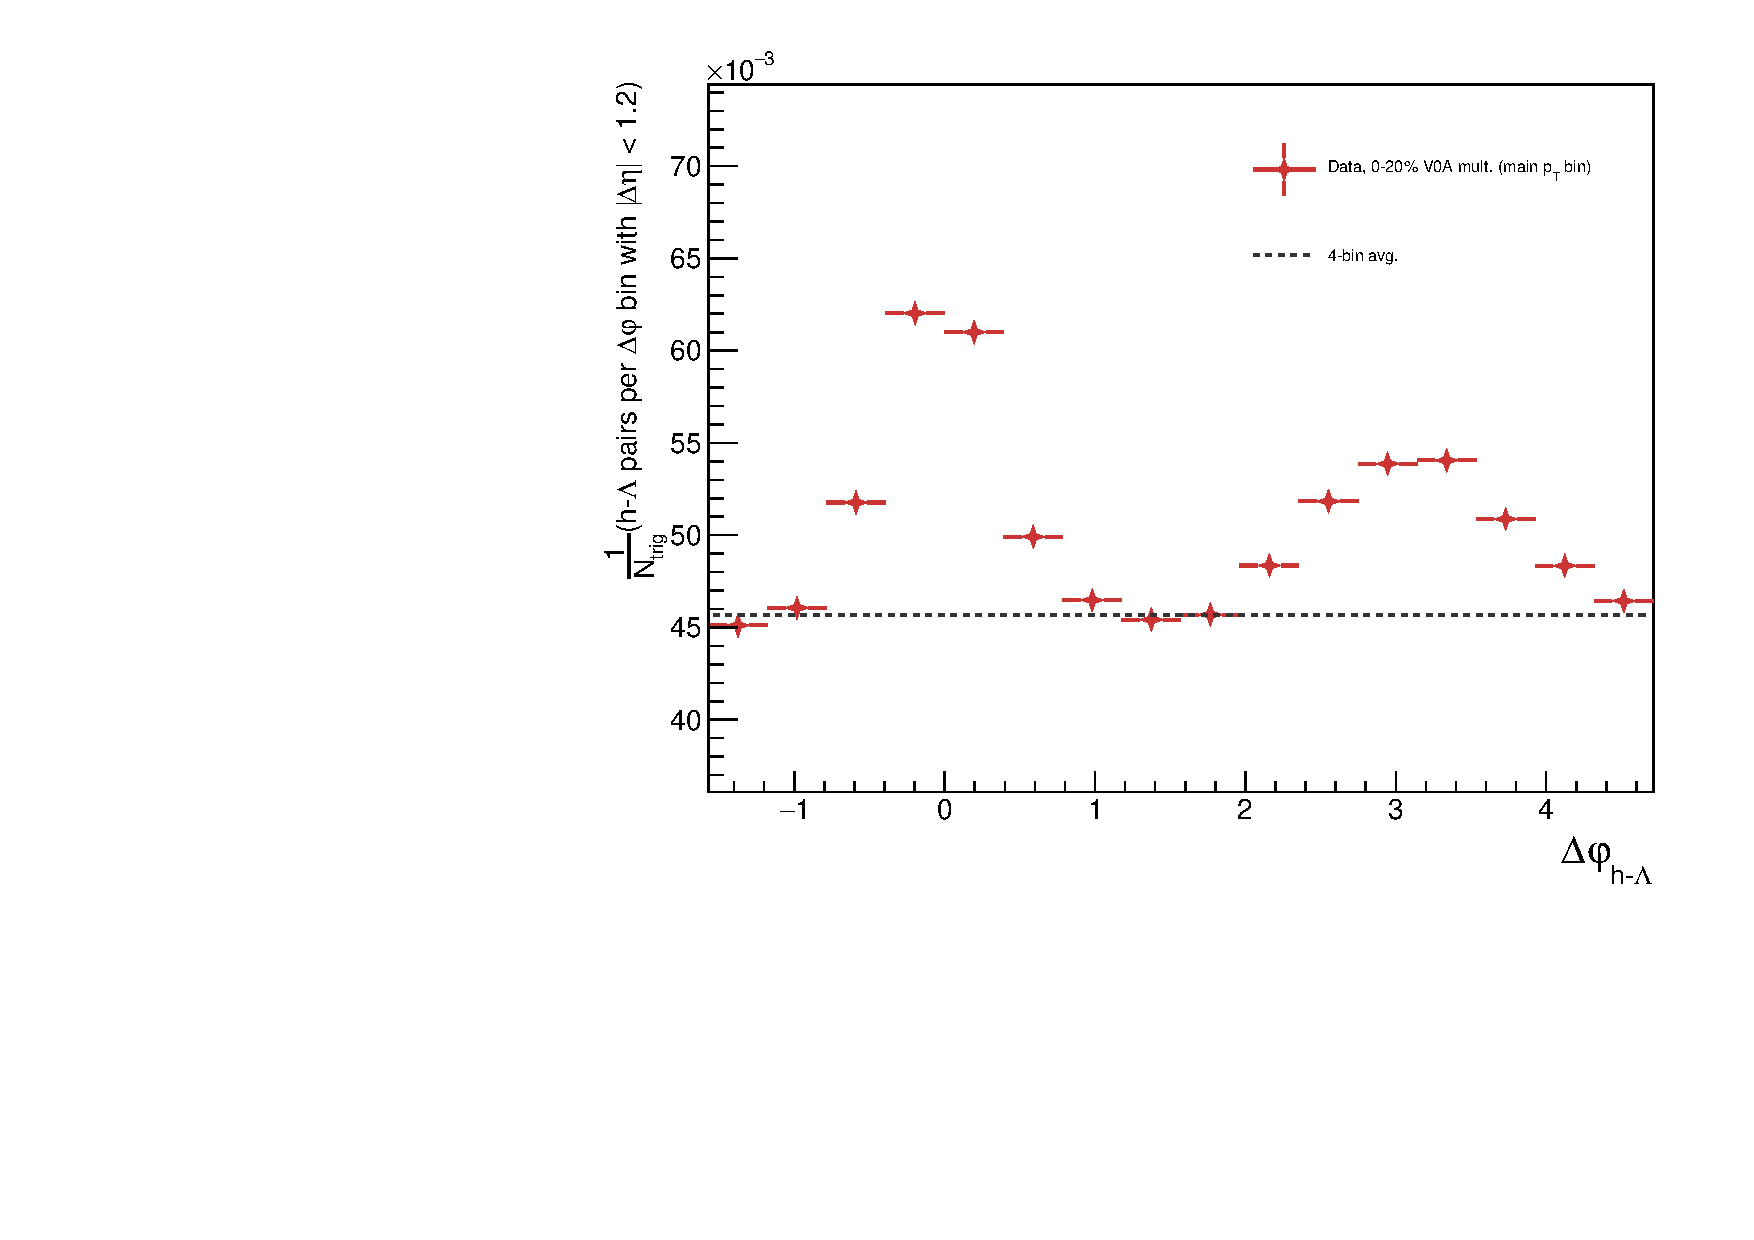
\includegraphics[width=4in]{figures/h_lambda_dphi_avg4_0_20.pdf}}
% \end{subfigure}
% \begin{subfigure}{
% \includegraphics[width=4in]{figures/h_lambda_dphi_avg4_20_50.pdf}}
% \end{subfigure}
% \begin{subfigure}{
% \includegraphics[width=4in]{figures/h_lambda_dphi_avg4_50_80.pdf}}
% \end{subfigure}
% \caption{The final per-trigger $h-\Lambda$ $\Delta\varphi$ correlations with underlying event fit for the 0-20\% (top), 20-50\%(center) and 50-80\% (bottom) multiplicity bins. The dashed line is the central value for the fit. The underlying event fit was taken using the 4-bin technique described in this section.} 
% \label{h_lambda_dphi_uefit_4bin}
% \end{figure}

%  \clearpage
 
% \begin{figure}[ht]
% \centering
% \begin{subfigure}{
% \includegraphics[width=4in]{figures/h_h_dphi_avg4_0_20.pdf}}
% \end{subfigure}
% \begin{subfigure}{
% \includegraphics[width=4in]{figures/h_h_dphi_avg4_20_50.pdf}}
% \end{subfigure}
% \begin{subfigure}{
% \includegraphics[width=4in]{figures/h_h_dphi_avg4_50_80.pdf}}
% \end{subfigure}
% \caption{The final per-trigger $h-h$ $\Delta\varphi$ correlations with underlying event fit for the 0-20\% (top), 20-50\%(center) and 50-80\% (bottom) multiplicity bins. The dashed line is the central value for the fit. The underlying event fit was taken using the 4-bin technique described in this section.} 
% \label{h_h_dphi_uefit_4bin}
% \end{figure}

% \clearpage



% \subsubsection{ZYAM Underlying Event Technique}
% \label{zyam}
% The ZYAM (Zero Yield At Minimum) underlying event technique is a modification of the 4 and 6 bin techniques, whereby we only take the minimum bin value in the $\Delta\varphi$ distribution as the underlying event value. The full technique is as follows:

% \begin{itemize}
% \item The underlying event region is defined using a straight-line fit with value and error set to the value and error of the minimum bin in the $\Delta\varphi$ distribution
% \item The near-side yield is calculated via $\sum_{i=1}^{8} (\Delta\varphi_\text{bin i} - \text{UE}_i)$, where $\text{UE}_i$ is the value of the straight-line fit at the center of the ith bin
% \item The away-side yield is calculated via $\sum_{i=9}^{16} (\Delta\varphi_\text{bin i} - \text{UE}_i)$, where $\text{UE}_i$ is the value of the straight-line fit at the center of the ith bin
% \item The underlying-event yield is calculated via $\sum_{i=1}^{16} \text{UE}_i = 16 \times UE$
% \item The total-yield is calculated via $\sum_{i=1}^{16} \Delta\varphi_\text{bin i} = \text{near-side} + \text{away-side} + \text{underlying-event}$
% \end{itemize}

% The final per-trigger $\Delta\varphi$ plots with the UE fit using the ZYAM UE technique are shown in Figures \ref{h_lambda_dphi_uefit_zyam} ($h-\Lambda$) and \ref{h_h_dphi_uefit_zyam} ($h-h$), and the extracted yields are shown in Table \ref{h_lambda_yield_table_zyam} ($h-\Lambda$) and Table \ref{h_h_yield_table_zyam} ($h-h$).

% \begin{table}[h!]
% \centering
% \begin{tabular}{| c || c | c | c | c | }
% \hline
% Multiplicity Bin & Near-side Jet & Away-side Jet & Underlying Event & Total  \\
% \hline
	
% 0-20\% & 4.69e-02  & 3.86e-02  & 7.22e-01 & 8.07e-01 \\
% 20-50\% & 3.63e-02 & 3.04e-02  & 3.82e-01 & 4.49e-01 \\
% 50-80\% & 2.84e-02 & 2.22e-02  & 1.88e-01 & 2.39e-01 \\
	
% \hline
% \end{tabular}
% \caption{Per-trigger pairwise $h-\Lambda$ extracted yields and corresponding statistical errors in the different kinematic regions for each multiplicity bin. The yields were extracted using the ZYAM technique described in this section. As these yields deviate the most from our central values, this will likely be the largest contribution to our systematic errors in the yield extraction.}
% \label{h_lambda_yield_table_zyam}
% \end{table}
	
% \begin{table}[h!]
% \centering
% \begin{tabular}{| c || c | c | c | c | }
% \hline
% Multiplicity Bin & Near-side Jet & Away-side Jet & Underlying Event & Total  \\
% \hline

% 0-20\% & 3.77e-01  & 2.53e-01  & 3.49e+00 & 4.12e+00 \\
% 20-50\% & 3.54e-01 & 2.25e-01  & 2.09e+00 & 2.67e+00 \\
% 50-80\% & 3.52e-01 & 2.11e-01  & 1.16e+00 & 1.73e+00 \\

% \hline
% \end{tabular}
% \caption{Per-trigger pairwise $h-h$ extracted yields and corresponding statistical errors in the different kinematic regions for each multiplicity bin. The yields were extracted using the ZYAM technique described in this section.}
% \label{h_h_yield_table_zyam}
% \end{table}

% \clearpage

% \begin{figure}[ht]
% \centering
% \begin{subfigure}{
% \includegraphics[width=4in]{figures/h_lambda_dphi_zyam_0_20.pdf}}
% \end{subfigure}
% \begin{subfigure}{
% \includegraphics[width=4in]{figures/h_lambda_dphi_zyam_20_50.pdf}}
% \end{subfigure}
% \begin{subfigure}{
% \includegraphics[width=4in]{figures/h_lambda_dphi_zyam_50_80.pdf}}
% \end{subfigure}
% \caption{The final per-trigger $h-\Lambda$ $\Delta\varphi$ correlations with underlying event fit for the 0-20\% (top), 20-50\%(center) and 50-80\% (bottom) multiplicity bins. The dashed line is the central value for the fit. The underlying event fit was taken using the ZYAM technique described in this section.} 
% \label{h_lambda_dphi_uefit_zyam}
% \end{figure}
	
% \begin{figure}[ht]
% \centering
% \begin{subfigure}{
% \includegraphics[width=4in]{figures/h_h_dphi_zyam_0_20.pdf}}
% \end{subfigure}
% \begin{subfigure}{
% \includegraphics[width=4in]{figures/h_h_dphi_zyam_20_50.pdf}}
% \end{subfigure}
% \begin{subfigure}{
% \includegraphics[width=4in]{figures/h_h_dphi_zyam_50_80.pdf}}
% \end{subfigure}
% \caption{The final per-trigger $h-h$ $\Delta\varphi$ correlations with underlying event fit for the 0-20\% (top), 20-50\%(center) and 50-80\% (bottom) multiplicity bins. The dashed line is the central value for the fit. The underlying event fit was taken using the ZYAM technique described in this section.} 
% \label{h_h_dphi_uefit_zyam}
% \end{figure}

% \clearpage

% \subsubsection{6-bin Underlying Event Technique With Non-Negative Constraint}
% \label{6binnonneg}
% We again consider the 6-bin underlying event technique, but we restrict that each term in $\sum_{i=1}^{8} (\Delta\varphi_\text{bin i} - \text{UE}_i)$ (near-side yield) and $\sum_{i=9}^{16} (\Delta\varphi_\text{bin i} - \text{UE}_i)$ (away side yield) is non-negative, as ``negative'' contributions to the yield are unphysical. The full technique is as follows:

% \begin{itemize}
% \item The underlying event region is defined using a straight-line fit of the average of bins (1, 2, 7, 8, 9, 16) in the $\Delta\varphi$ distribution
% \item The near-side yield is calculated via $\sum_{i=1}^{8} (\Delta\varphi_\text{bin i} - \text{UE}_i)$, where $\text{UE}_i$ is the value of the straight-line fit at the center of the ith bin and all negative terms in the sum are manually set to zero
% \item The away-side yield is calculated via $\sum_{i=9}^{16} (\Delta\varphi_\text{bin i} - \text{UE}_i)$, where $\text{UE}_i$ is the value of the straight-line fit at the center of the ith bin and all negative terms in the sum are manually set to zero
% \item The underlying-event yield is calculated via $\sum_{i=1}^{16} \text{UE}_i = 16 \times UE$
% \item The total-yield is calculated via $\sum_{i=1}^{16} \Delta\varphi_\text{bin i} = \text{near-side} + \text{away-side} + \text{underlying-event}$
% \end{itemize}

% As this method doesn't change the UE fit line in any way, we report only the extracted yields in Table \ref{h_lambda_yield_table_6bin_nonzero} ($h-\Lambda$) and Table \ref{h_h_yield_table_6bin_nonzero} ($h-h$). (If you would like a reminder of the $\Delta\varphi$ plots with 6-bin UE fits, see Figures \ref{v0_1d_correlations_with_fit} ($h-\Lambda$) and \ref{hh_1d_correlations_with_fit} ($h-h$))

	
% \begin{table}[h!]
% \centering
% \begin{tabular}{| c || c | c | c | c | }
% \hline
% Multiplicity Bin & Near-side Jet & Away-side Jet & Underlying Event & Total  \\
% \hline
	
% 0-20\% & 4.21e-02  & 3.27e-02  & 7.34e-01 & 8.07e-01 \\
% 20-50\% & 3.23e-02 & 2.55e-02  & 3.92e-01 & 4.49e-01 \\
% 50-80\% & 2.53e-02 & 1.89e-02  & 1.95e-01 & 2.39e-01 \\
	
% \hline
% \end{tabular}
% \caption{Per-trigger pairwise $h-\Lambda$ extracted yields and corresponding statistical errors in the different kinematic regions for each multiplicity bin. The yields were extracted using the 6-bin UE technique with non-negative constraint described in this section.}
% \label{h_lambda_yield_table_6bin_nonzero}
% \end{table}
	
% \begin{table}[h!]
% \centering
% \begin{tabular}{| c || c | c | c | c | }
% \hline
% Multiplicity Bin & Near-side Jet & Away-side Jet & Underlying Event & Total  \\
% \hline

% 0-20\% & 3.54e-01  & 2.24e-01  & 3.55e+00 & 4.12e+00 \\
% 20-50\% & 3.40e-01 & 2.06e-01  & 2.13e+00 & 2.67e+00 \\
% 50-80\% & 3.38e-01 & 1.92e-01  & 1.20e+00 & 1.73e+00 \\

% \hline
% \end{tabular}
% \caption{Per-trigger pairwise $h-h$ extracted yields and corresponding statistical errors in the different kinematic regions for each multiplicity bin. The yields were extracted using the 6-bin UE technique with non-negative constraint described in this section.}
% \label{h_h_yield_table_6bin_nonzero}
% \end{table}

% \clearpage

% \subsubsection{Full 1D Correlation Fit (2 Gaussians)}
% \label{full_correlation_fit}
% The full 1D correlation fit with two gaussians involves fitting the entire $\Delta\varphi$ distribution with a function that includes near-side, away-side and underlying-event components. The fit function is given by:

% \begin{gather*}
% 	\text{Fit}(\Delta\varphi) = C + A_{near}*\exp{\frac{(\Delta\varphi - M_{near})^2}{2*\sigma_{near}}} + A_{away}*\exp{\frac{(\Delta\varphi - M_{away})^2}{2*\sigma_{away}}} \\
% 	+ (A_{near,mirror}*\exp{\frac{((\Delta\varphi+2\pi) - M_{near,mirror})^2}{2*\sigma_{near,mirror}}} + A_{away,mirror}*\exp{\frac{((\Delta\varphi-2\pi) - M_{away,mirror})^2}{2*\sigma_{away,mirror}}})
% \end{gather*}

% where the ``mirror'' terms are added to account for the $2\pi$ periodicity of the $\Delta\varphi$ distribution. The mean in the near-side gaussian (and corresponding mirror term) is fixed to 0 ($2\pi$) and the mean in the away-side guassian (and corresponding mirror term) is fixed to $\pi$ ($-\pi$), but all other parameters are allowed to vary. The yield extraction procedure is as follows:

% \begin{itemize}
% \item The $\Delta\varphi$ distribution is fit with the correlation function described above in the range $\frac{-\pi}{2} < \Delta\varphi < \frac{3\pi}{2}$
% \item The near-side yield is calculated via $\frac{16}{2\pi}(\int_{\frac{-\pi}{2}}^{\frac{\pi}{2}}Fit(\Delta\varphi)d\Delta\varphi - \int_{\frac{-\pi}{2}}^{\frac{\pi}{2}}UE d\Delta\varphi)$, where UE is a constant calculated from the average of bins (1, 2, 7, 8, 9, 16)
% \item The away-side yield is calculated via $\frac{16}{2\pi}(\int_{\frac{\pi}{2}}^{\frac{3\pi}{2}}Fit(\Delta\varphi)d\Delta\varphi - \int_{\frac{\pi}{2}}^{\frac{3\pi}{2}}UE d\Delta\varphi)$
% \item The underlying-event yield is calculated via $\frac{16}{2\pi}\int_{\frac{-\pi}{2}}^{\frac{3\pi}{2}}UE d\Delta\varphi$
% \item The total yield is calculated via $\frac{16}{2\pi}\int_{\frac{-\pi}{2}}^{\frac{3\pi}{2}}Fit(\Delta\varphi) d\Delta\varphi$
% \end{itemize}

% The constant $\frac{16}{2\pi}$ being multiplied by each term is just the inverse of the bin width ($2\pi$ radians for 16 $\Delta\varphi$ bins).
% The final per-trigger $\Delta\varphi$ plots with the full correlation fits are shown in Figures \ref{h_lambda_dphi_fullfit} ($h-\Lambda$) and \ref{h_h_dphi_fullfit} ($h-h$), and the extracted yields are shown in Table \ref{h_lambda_yield_table_fullfit} ($h-\Lambda$) and Table \ref{h_h_yield_table_fullfit} ($h-h$). It's worth nothing that the yields are extremely similar to those from our central technique, as the UE is the same and the fits are very good.

% \begin{table}[h!]
% \centering
% \begin{tabular}{| c | c | c | c | c | }
% \hline
% Multiplicity Bin & Near-side Jet & Away-side Jet & Underlying Event & Total  \\
% \hline
	
% 0-20\% & 4.07e-02  & 3.26e-02  & 7.34e-01 & 8.07e-01 \\
% 20-50\% & 3.11e-02 & 2.55e-02  & 3.92e-01 & 4.49e-01 \\
% 50-80\% & 2.44e-02 & 1.88e-02  & 1.95e-01 & 2.38e-01 \\
	
% \hline
% \end{tabular}
% \caption{Per-trigger pairwise $h-\Lambda$ extracted yields in the different kinematic regions for each multiplicity bin. The yields were extracted using the full correlation fit procedure described in this section.}
% \label{h_lambda_yield_table_fullfit}
% \end{table}
	
% \begin{table}[h!]
% \centering
% \begin{tabular}{| c | c | c | c | c | }
% \hline
% Multiplicity Bin & Near-side Jet & Away-side Jet & Underlying Event & Total  \\
% \hline

% 0-20\% & 3.48e-01  & 2.24e-01  & 3.55e+00 & 4.12e+00 \\
% 20-50\% & 3.36e-01 & 2.05e-01  & 2.13e+00 & 2.67e+00 \\
% 50-80\% & 3.35e-01 & 1.90e-01  & 1.20e+00 & 1.73e+00 \\

% \hline
% \end{tabular}
% \caption{Per-trigger pairwise $h-h$ extracted yields in the different kinematic regions for each multiplicity bin. The yields were extracted using the full correlation fit procedure described in this section.}
% \label{h_h_yield_table_fullfit}
% \end{table}

% \clearpage

% \begin{figure}[ht]
% \centering
% \begin{subfigure}{
% \includegraphics[width=4in]{figures/h_lambda_dphi_gaus_0_20.pdf}}
% \end{subfigure}
% \begin{subfigure}{
% \includegraphics[width=4in]{figures/h_lambda_dphi_gaus_20_50.pdf}}
% \end{subfigure}
% \begin{subfigure}{
% \includegraphics[width=4in]{figures/h_lambda_dphi_gaus_50_80.pdf}}
% \end{subfigure}
% \caption{The final per-trigger $h-\Lambda$ $\Delta\varphi$ correlations with the full 2xGaussian fit for the 0-20\% (top), 20-50\%(center) and 50-80\% (bottom) multiplicity bins. The fit was generated using the technique described in this section.}
% \label{h_lambda_dphi_fullfit}
% \end{figure}
	
% \begin{figure}[ht]
% \centering
% \begin{subfigure}{
% \includegraphics[width=4in]{figures/h_h_dphi_gaus_0_20.pdf}}
% \end{subfigure}
% \begin{subfigure}{
% \includegraphics[width=4in]{figures/h_h_dphi_gaus_20_50.pdf}}
% \end{subfigure}
% \begin{subfigure}{
% \includegraphics[width=4in]{figures/h_h_dphi_gaus_50_80.pdf}}
% \end{subfigure}
% \caption{The final per-trigger $h-h$ $\Delta\varphi$ correlations with the full 2xGaussian fit for the 0-20\% (top), 20-50\%(center) and 50-80\% (bottom) multiplicity bins. The fit was generated using the technique described in this section.}
% \label{h_h_dphi_fullfit}
% \end{figure}

% \clearpage

% \subsubsection{Including $v_{2}$ (Von Mises and just $v_{2}$)}
% \label{including_v2}
% For the final two techniques, we investigate the inclusion of a non-zero $v_{2}$ (which is definitely the case, especially in our 0-20\% multiplicity bin). First, the $v_{2}$ values are determined as a function of $p_{T}$ from Figure 31 in this AN: \url{https://alice-notes.web.cern.ch/system/files/notes/analysis/1228/2022-09-15-AN_PIDflowInSmallSystems_v4.pdf}. As our $p_{T}$ binning is much wider, we then take the weighted average across each of our $p_{T}$ bins using the published $p_{T}$ spectra for charged hadrons and $\Lambda$s from HEPData (found here: \url{https://www.hepdata.net/record/ins1244523?version=2}). The final values in the 0-20\% multiplicity bin for each $p_{T, assoc}$ bin are shown in Table \ref{v2_table}. 

% \begin{table}[h!]
% \centering
% \begin{tabular}{| c || c | c | c | c | }
% \hline
% $p_{T, assoc}$ & $v_{2}^{trigger}$ & $v_{2}^{assoc h}$ & $v_{2}^{assoc \Lambda}$ \\
% \hline
% 2.0 - 4.0 & 0.092 & 0.112 & 0.111 \\
% 1.5 - 2.5 & 0.092 & 0.100 & 0.075 \\
% 2.5 - 4.0 & 0.092 & 0.119 & 0.137 \\
% \hline
% \end{tabular}
% \caption{$v_{2}$ values used in this analysis for each $p_{T, assoc}$ bin.}
% \label{v2_table}
% \end{table}

% As there is no data available for the 20-50\% and 50-80\% multiplicity bins, we take 0.85 and 0.5 times the 0-20\% value, respectively. 

% Using these $v_{2}$ values, we then fit the following function to the $\Delta\varphi$ distribution in the regions $-\pi/2 < \Delta\varphi < -1$ and $1 < \Delta\varphi < +\pi/2$ (i.e., regions with little-to-no jet components). The fit function is given by:

% \begin{equation}
% Fit_{v_{2}}(\Delta\varphi) = A\times(1 + 2v_{2, trig}v_{2, assoc}cos(2\Delta\varphi))
% \end{equation}

% where A is the underlying event pedestal, which is allowed to vary during the fit. The $v_{2}$ values are fixed to the values in Table \ref{v2_table}. The final two techniques both use the same fit function for the UE.

% \subsubsection{Full 1D Correlation Fit (Von Mises with $v_{2}$)}
% \label{full_correlation_fit_von}
% The full 1D correlation fit with  Von Mises involves fitting the entire $\Delta\varphi$ distribution with a function that includes near-side, away-side and underlying-event components. The fit function is given by:

% \begin{gather*}
% 	\text{Fit}(\Delta\varphi) = Fit_{v_{2}} +
% 	(\frac{1}{2\pi I_{0}(\kappa_{near})})e^{\kappa_{near} \cos(\Delta\varphi)} +  \\
% 	(\frac{1}{2\pi I_{0}(\kappa_{away})})e^{\kappa_{away} \cos(\Delta\varphi)} 
% \end{gather*}

% where $Fit_{v_{2}}$ is fixed using the procedure described in the previous section (\ref{including_v2}) and I$_0$ is the modified Bessel function of zero order. All other parameters are allowed to vary. The full technique is as follows:

% \begin{itemize}
% \item The $\Delta\varphi$ distribution is fit with the correlation function described above in the range $\frac{-\pi}{2} < \Delta\varphi < \frac{3\pi}{2}$
% \item The near-side yield is calculated via $\frac{16}{2\pi}(\int_{\frac{-\pi}{2}}^{\frac{\pi}{2}}Fit(\Delta\varphi)d\Delta\varphi - \int_{\frac{-\pi}{2}}^{\frac{\pi}{2}}Fit_{v_{2}}(\Delta\varphi) d\Delta\varphi)$
% \item The away-side yield is calculated via $\frac{16}{2\pi}(\int_{\frac{\pi}{2}}^{\frac{3\pi}{2}}Fit(\Delta\varphi)d\Delta\varphi - \int_{\frac{\pi}{2}}^{\frac{3\pi}{2}}Fit_{v_{2}}(\Delta\varphi)\Delta\varphi)$
% \item The underlying-event yield is calculated via $\frac{16}{2\pi}\int_{\frac{-\pi}{2}}^{\frac{3\pi}{2}}Fit_{v_{2}}(\Delta\varphi) d\Delta\varphi$
% \item The total yield is calculated via $\frac{16}{2\pi}\int_{\frac{-\pi}{2}}^{\frac{3\pi}{2}}Fit(\Delta\varphi) d\Delta\varphi$
% \end{itemize}

% The constant $\frac{16}{2\pi}$ being multiplied by each term is just the inverse of the bin width ($2\pi$ radians for 16 $\Delta\varphi$ bins).
% The final per-trigger $\Delta\varphi$ plots with the full Von Mises fits and $v_{2}$ assumptions shown in Figures \ref{h_lambda_dphi_vonfit} ($h-\Lambda$) and \ref{h_h_dphi_vonfit} ($h-h$), and the extracted yields are shown in Table \ref{h_lambda_yield_table_vonfit} ($h-\Lambda$) and Table \ref{h_h_yield_table_vonfit} ($h-h$). 

% \begin{table}[h!]
% \centering
% \begin{tabular}{| c || c | c | c | c | }
% \hline
% Multiplicity Bin & Near-side Jet & Away-side Jet & Underlying Event & Total  \\
% \hline
	
% 0-20\% & 3.87e-02  & 3.03e-02  & 7.38e-01 & 8.07e-01 \\
% 20-50\% & 3.27e-02 & 2.69e-02  & 3.89e-01 & 4.49e-01 \\
% 50-80\% & 2.60e-02 & 2.04e-02  & 1.92e-01 & 2.38e-01 \\
	
% \hline
% \end{tabular}
% \caption{Per-trigger pairwise $h-\Lambda$ extracted yields in the different kinematic regions for each multiplicity bin. The yields were extracted using the full Von Mises fit procedure described in this section.}
% \label{h_lambda_yield_table_vonfit}
% \end{table}
	
% \begin{table}[h!]
% \centering
% \begin{tabular}{| c || c | c | c | c | }
% \hline
% Multiplicity Bin & Near-side Jet & Away-side Jet & Underlying Event & Total  \\
% \hline

% 0-20\% & 3.41e-01  & 2.15e-01  & 3.57e+00 & 4.12e+00 \\
% 20-50\% & 3.40e-01 & 2.08e-01  & 2.12e+00 & 2.67e+00 \\
% 50-80\% & 3.49e-01 & 2.04e-01  & 1.17e+00 & 1.73e+00 \\

% \hline
% \end{tabular}
% \caption{Per-trigger pairwise $h-h$ extracted yields in the different kinematic regions for each multiplicity bin. The yields were extracted using the full Von Mises fit procedure described in this section.}
% \label{h_h_yield_table_vonfit}
% \end{table}

% \clearpage

% \begin{figure}[ht]
% \centering
% \begin{subfigure}{
% \includegraphics[width=4in]{figures/h_lambda_dphi_von_0_20.pdf}}
% \end{subfigure}
% \begin{subfigure}{
% \includegraphics[width=4in]{figures/h_lambda_dphi_von_20_50.pdf}}
% \end{subfigure}
% \begin{subfigure}{
% \includegraphics[width=4in]{figures/h_lambda_dphi_von_50_80.pdf}}
% \end{subfigure}
% \caption{The final per-trigger $h-\Lambda$ $\Delta\varphi$ correlations with the full Von Mises fit for the 0-20\% (top), 20-50\%(center) and 50-80\% (bottom) multiplicity bins. The fit was generated using the technique described in this section.}
% \label{h_lambda_dphi_vonfit}
% \end{figure}
	
% \begin{figure}[ht]
% \centering
% \begin{subfigure}{
% \includegraphics[width=4in]{figures/h_h_dphi_von_0_20.pdf}}
% \end{subfigure}
% \begin{subfigure}{
% \includegraphics[width=4in]{figures/h_h_dphi_von_20_50.pdf}}
% \end{subfigure}
% \begin{subfigure}{
% \includegraphics[width=4in]{figures/h_h_dphi_von_50_80.pdf}}
% \end{subfigure}
% \caption{The final per-trigger $h-h$ $\Delta\varphi$ correlations with the full Von Mises fit for the 0-20\% (top), 20-50\%(center) and 50-80\% (bottom) multiplicity bins. The fit was generated using the technique described in this section.}
% \label{h_h_dphi_vonfit}
% \end{figure}

% \clearpage


% \subsubsection{Just $v_{2}$}
% \label{v2_background_technique}
% For this technique, we repeat the same procedure as the Von Mises technique, but we use bin-wise integration to extract the yields (i.e. we do not use the full Von Mises fit). The yields are extracted using the following method:

% \begin{itemize}
% \item Let $Fit_{v_{2}}(\Delta\varphi) = A\times(1 + 2v_{2, trig}v_{2, assoc}cos(2\Delta\varphi))$, where this is fit using the technique described in Section \ref{including_v2}
% \item The near-side yield is calculated via $\sum_{i=1}^{8} (\Delta\varphi_\text{bin i} - Fit_{v_{2}, \text{bin i}})$, where $Fit_{v_{2}, \text{bin i}}$ is the value of $Fit_{v_{2}}$ at the center of the ith $\Delta\varphi$ bin
% \item The away-side yield is calculated via $\sum_{i=8}^{16} (\Delta\varphi_\text{bin i} - Fit_{v_{2}, \text{bin i}})$
% \item The underlying-event yield is calculated via $\frac{16}{2\pi}\int_{\frac{-\pi}{2}}^{\frac{3\pi}{2}} Fit_{v_{2}} d\Delta\varphi$
% \item The total-yield is calculated via $\sum_{i=1}^{16} \Delta\varphi_\text{bin i} = \text{near-side} + \text{away-side} + \text{underlying-event}$
% \end{itemize}

% The constant $\frac{16}{2\pi}$ being multiplied by the underlying event integral term is just the inverse of the bin width ($2\pi$ radians for 16 $\Delta\varphi$ bins). The final per-trigger $\Delta\varphi$ plots with the $v_{2}$ fits are shown in Figures \ref{h_lambda_dphi_v2fit} ($h-\Lambda$) and \ref{h_h_dphi_v2fit} ($h-h$), and the extracted yields are shown in Table \ref{h_lambda_yield_table_v2fit} ($h-\Lambda$) and Table \ref{h_h_yield_table_v2fit} ($h-h$). 

% \begin{table}[h!]
% \centering
% \begin{tabular}{| c || c | c | c | c | }
% \hline
% Multiplicity Bin & Near-side Jet & Away-side Jet & Underlying Event & Total  \\
% \hline
% 0-20\% & 3.87e-02  & 3.04e-02  & 7.38e-01 & 8.07e-01 \\
% 20-50\% & 3.28e-02 & 2.69e-02  & 3.89e-01 & 4.49e-01 \\
% 50-80\% & 2.63e-02 & 2.02e-02  & 1.92e-01 & 2.39e-01 \\
% \hline
% \end{tabular}
% \caption{Per-trigger pairwise $h-\Lambda$ extracted yields in the different kinematic regions for each multiplicity bin. The yields were extracted using the $v_{2}$ fit procedure described in this section. Despite the optically large contribution from $v_{2}$ in the most central multiplicity bin, the extracted yields are still very similar to the other techniques.}
% \label{h_lambda_yield_table_v2fit}
% \end{table}

% \clearpage

% \begin{figure}[ht]
% \centering
% \begin{subfigure}{
% \includegraphics[width=4in]{figures/h_lambda_dphi_v2_0_20.pdf}}
% \end{subfigure}
% \begin{subfigure}{
% \includegraphics[width=4in]{figures/h_lambda_dphi_v2_20_50.pdf}}
% \end{subfigure}
% \begin{subfigure}{
% \includegraphics[width=4in]{figures/h_lambda_dphi_v2_50_80.pdf}}
% \end{subfigure}
% \caption{The final per-trigger $h-\Lambda$ $\Delta\varphi$ correlations with the $v_2$ fit for the 0-20\% (top), 20-50\%(center) and 50-80\% (bottom) multiplicity bins. The $v_2$ fit was generated using the technique described in this section. The most central multiplicity bin sees a substantial contribution from $v_{2}$, whereas the other bins only see a small contribution.}
% \label{h_lambda_dphi_v2fit}
% \end{figure}

% \begin{figure}[ht]
% \centering
% \begin{subfigure}{
% \includegraphics[width=4in]{figures/h_h_dphi_v2_0_20.pdf}}
% \end{subfigure}
% \begin{subfigure}{
% \includegraphics[width=4in]{figures/h_h_dphi_v2_20_50.pdf}}
% \end{subfigure}
% \begin{subfigure}{
% \includegraphics[width=4in]{figures/h_h_dphi_v2_50_80.pdf}}
% \end{subfigure}
% \caption{The final per-trigger $h-h$ $\Delta\varphi$ correlations with the $v_{2}$ fit for the 0-20\% (top), 20-50\%(center) and 50-80\% (bottom) multiplicity bins. The fit was generated using the technique described in this section. All multiplicity bins see a mostly negligible contribution from $v_{2}$.}
% \label{h_h_dphi_v2fit}
% \end{figure}

% \clearpage

% \begin{table}[h!]
% \centering
% \begin{tabular}{| c || c | c | c | c | }
% \hline
% Multiplicity Bin & Near-side Jet & Away-side Jet & Underlying Event & Total  \\
% \hline
% 0-20\% & 3.39e-01  & 2.16e-01  & 3.57e+00 & 4.12e+00 \\
% 20-50\% & 3.38e-01 & 2.09e-01  & 2.12e+00 & 2.67e+00 \\
% 50-80\% & 3.47e-01 & 2.06e-01  & 1.17e+00 & 1.73e+00 \\
% \hline
% \end{tabular}
% \caption{Per-trigger pairwise $h-h$ extracted yields in the different kinematic regions for each multiplicity bin. The yields were extracted using the $v_{2}$ fit procedure described in this section.}
% \label{h_h_yield_table_v2fit}
% \end{table}

% \subsubsection{Barlow Check (yield extraction)}
% \label{barlow_check_yield}
% For the yield extraction technique variations, we repeat the same Barlow check procedure as described in Section \ref{barlow_check_dphi}, where for each kinematic region we calculate:
% \begin{equation}
% 	N\sigma_{RB} := \frac{y_{var} - y_{central}}{\sqrt{|\sigma_{var}^2 - \sigma_{central}^2|}},
% \end{equation}

%  Again, we just count the number of kinematic regions that have $|N\sigma_{RB}| < 1$, and if this is the majority of the regions (across ALL multiplicity and $p_{T, assoc}$ bins), we exclude the variation from our systematic calculation. The plots of $N\sigma_{RB}$ for each variation in our 0-20\% multiplicity bin for each $p_{T, assoc}$ bin are shown in Figure \ref{barlow_check_0_20}. The red lines represent $N\sigma_{RB} = \pm 1$.

% As a result of the check, the following variations were excluded from our systematic calculation:
% \begin{itemize}
% \item Double Gaussian
% \item Von Mises
% \end{itemize}

% The exclusion of the Double Gaussian fit technique comes directly from the test: as we use the same UE (6 bin average) with this technique as we do for our central point, and the fits are very nice, the resulting yields end up being extremely similar. The exclusion of Von Mises comes from the fact that the results are nearly identical to the ones obtained by just including the $v_{2}$ fit and doing bin-wise integration. Again, this is because the Von Mises fit describes the data very well, so including it along with just the $v_{2}$ fit is redundant. All 36 fits for the Von Mises and Double Gaussian techniques behave very well, with nice error matrices, and will therefore be saved for a rainy day (or for future studies).

% Every technique excluded from the $h-\Lambda$ yield extraction systematic uncertainty calculation is also excluded from the $h-h$ yield extraction systematic uncertainty calculation.

% \clearpage 

% \begin{figure}[ht]
% \centering
% \begin{subfigure}{
% \includegraphics[width=4in]{figures/h_lambda_yield_barlow_0_20.pdf}}
% \end{subfigure}
% \begin{subfigure}{
% \includegraphics[width=4in]{figures/h_lambda_yield_barlow_0_20_lowpt.pdf}}
% \end{subfigure}
% \begin{subfigure}{
% \includegraphics[width=4in]{figures/h_lambda_yield_barlow_0_20_highpt.pdf}}
% \end{subfigure}
% \caption{Barlow check for the yield extraction techniques in the 0-20\% multiplicity bin. The top plot shows the $N\sigma_{RB}$ for the  $2 < p_{T, assoc} < 4$ GeV/c region, the middle plot shows the $N\sigma_{RB}$ for the  $1.5 < p_{T, assoc} < 2.5$ GeV/c region, and the bottom plot shows the $N\sigma_{RB}$ for the  $2.5 < p_{T, assoc} < 4$ GeV/c region. The red lines represent $N\sigma_{RB} = \pm 1$, and if the majority of the points for a given variation fall within those lines (across all multiplicity and $p_{T}$ bins), that variation is excluded from the systematic uncertainty calculation.}
% \label{barlow_check_yield_0_20}
% \end{figure}

% \clearpage 

% \subsubsection{ZYAM aside}
% \label{zyam_aside}
% While the ZYAM technique was initially considered as it is a fairly common yield extraction technique in pp correlation studies, it is \textit{physically} incompatible with the presence of $v_{2}$, which is certainly the case in high multiplicity p--Pb. We can see this very clearly in the 0-20\% bins of Figures \ref{h_lambda_dphi_v2fit} ($v_{2}$ inclusion) and \ref{h_lambda_dphi_uefit_zyam} (ZYAM), where the ``pedestal'' obtained by ZYAM is clearly not compatible with the pedestal obtained by the $v_{2}$ fit (draw a line through the center of the oscillations). Furthermore, from looking at the near-side and away-side yields obtained in the yield tables, we see that ZYAM deviates more than 15\% from our central values. Because of this, we do not consider ZYAM as a viable yield extraction technique and thus exclude it from our systematic uncertainty calculation.


% \subsubsection{Deviations from Central Values}
% In this section, we present the deviations from the central values for the yield extraction techniques in our 0-20\% multiplicity bin for each $p_{T, assoc}$ bin. The deviations are trivially calculated by $\frac{y_{var}}{y_{central}} - 1$, and are shown in Figures \ref{h_lambda_yield_deviations_0_20} ($h-\Lambda$) and \ref{h_h_yield_deviations_0_20} ($h-h$). 

% \clearpage

% \begin{figure}[ht]
% \centering
% \begin{subfigure}{
% \includegraphics[width=4in]{figures/h_lambda_0_20_yield_variation.pdf}}
% \end{subfigure}
% \begin{subfigure}{
% \includegraphics[width=4in]{figures/h_lambda_0_20_lowpt_yield_variation.pdf}}
% \end{subfigure}
% \begin{subfigure}{
% \includegraphics[width=4in]{figures/h_lambda_0_20_highpt_yield_variation.pdf}}
% \end{subfigure}
% \caption{Deviations from central values for the $h-\Lambda$ yield extraction techniques in the 0-20\% multiplicity bin for the central (top), lower (middle), and higher (bottom) $p_{T, assoc}$ bins.}
% \label{h_lambda_yield_deviations_0_20}
% \end{figure}

% \clearpage

% \begin{figure}[ht]
% \centering
% \begin{subfigure}{
% \includegraphics[width=4in]{figures/h_h_0_20_yield_variation.pdf}}
% \end{subfigure}
% \begin{subfigure}{
% \includegraphics[width=4in]{figures/h_h_0_20_lowpt_yield_variation.pdf}}
% \end{subfigure}
% \begin{subfigure}{
% \includegraphics[width=4in]{figures/h_h_0_20_highpt_yield_variation.pdf}}
% \end{subfigure}
% \caption{Deviations from central values for the $h-h$ yield extraction techniques in the 0-20\% multiplicity bin for the central (top), lower (middle), and higher (bottom) $p_{T, assoc}$ bins.}
% \label{h_h_yield_deviations_0_20}
% \end{figure}

% \clearpage


% \subsubsection{Final Systematic Errors from Yield Extraction}
% \label{final_systematic_errors_yield_extraction}
% The final systematic errors for the yield extraction are calculated in the following way:

% \begin{itemize}
% \item For every yield extraction technique, the yield in a given kinematic region is divided by the yield in the same region using our default technique (6-bin UE)
% \item This procedure is done for each of the variations (PID, signal region, sideband region)
% \item The RMS of the resulting ratios in each kinematic region is calculated
% \end{itemize}

% The final systematic errors from the yield extraction in each kinematic region and multiplicity bin for the  $2 < p_{T, assoc} < 4$ GeV/c region can be seen in Tables \ref{h_lambda_yield_extraction_systematics} ($h-\Lambda$) and \ref{h_h_yield_extraction_systematics} ($h-h$). The same tables for the  $1.5 < p_{T, assoc} < 2.5$ GeV/c and  $1.5 < p_{T, assoc} < 2.5$ regions can also be seen starting at Table \ref{h_lambda_yield_extraction_systematics_lowpt}. 

% All systematic errors are reported in percentages. For the final ratio calculations, the $h-\Lambda$ and $h-h$ systematic errors are treated as uncorrelated.

% \begin{table}[h!]
% \centering
% \begin{tabular}{| c | c | c | c | c | }
% \hline
% Multiplicity Bin & Near-side Jet & Away-side Jet & Underlying Event & Total  \\
% \hline

% 0-20\% & 5.19e+00 & 5.70e+00  & 3.13e+00 & 3.10e+00 \\
% 20-50\% & 5.67e+00 & 6.15e+00  & 3.27e+00 & 3.20e+00 \\
% 50-80\% & 6.21e+00 & 7.51e+00  & 3.81e+00 & 3.60e+00 \\

% \hline
% \end{tabular}
% \caption{Final systematic errors from the $h-\Lambda$ yield extraction in each kinematic region and multiplicity bin, taken in the momentum range $2 < p_{T}^{\Lambda} < 4$ GeV/c. The systematic errors are calculated using the method described in this section.}
% \label{h_lambda_yield_extraction_systematics}
% \end{table}

% \begin{table}[h!]
% \centering
% \begin{tabular}{| c | c | c | c | c | }
% \hline
% Multiplicity Bin & Near-side Jet & Away-side Jet & Underlying Event & Total  \\
% \hline

% 0-20\% & 3.93e+00   & 4.15e+00  & 3.51e+00 & 3.50e+00 \\
% 20-50\% & 3.64e+00 & 3.62e+00  & 3.50e+00 & 3.50e+00 \\
% 50-80\% & 4.33e+00 & 5.41e+00  & 3.74e+00 & 3.50e+00 \\

% \hline
% \end{tabular}
% \caption{Final systematic errors from the $h-h$ yield extraction in each kinematic region and multiplicity bin, taken in the momentum range $2 < p_{T}^{h} < 4$ GeV/c. The systematic errors are calculated using the method described in this section.}
% \label{h_h_yield_extraction_systematics}
% \end{table}

% \begin{table}[h!]
% \centering
% \begin{tabular}{| c | c | c | c | c | }
% \hline
% Multiplicity Bin & Near-side Jet & Away-side Jet & Underlying Event & Total  \\
% \hline

% 0-20\% & 5.50e+00 & 5.57e+00  & 3.12e+00 & 3.10e+00 \\
% 20-50\% & 4.94e+00 & 5.24e+00  & 3.22e+00 & 3.20e+00 \\
% 50-80\% & 6.34e+00 & 7.19e+00  & 3.68e+00 & 3.60e+00 \\

% \hline
% \end{tabular}
% \caption{Final systematic errors from the $h-\Lambda$ yield extraction in each kinematic region and multiplicity bin, taken in the momentum range $1.5 < p_{T}^{\Lambda} < 2.5$ GeV/c. The systematic errors are calculated using the method described in this section.}
% \label{h_lambda_yield_extraction_systematics_lowpt}
% \end{table}

% \begin{table}[h!]
% \centering
% \begin{tabular}{| c | c | c | c | c | }
% \hline
% Multiplicity Bin & Near-side Jet & Away-side Jet & Underlying Event & Total  \\
% \hline

% 0-20\% & 4.46e+00   & 4.75e+00  & 3.51e+00 & 3.50e+00 \\
% 20-50\% & 3.75e+00 & 3.63e+00  & 3.50e+00 & 3.50e+00 \\
% 50-80\% & 4.94e+00 & 6.35e+00  & 3.67e+00 & 3.50e+00 \\

% \hline
% \end{tabular}
% \caption{Final systematic errors from the $h-h$ yield extraction in each kinematic region and multiplicity bin, taken in the momentum range $1.5 < p_{T}^{h} < 2.5$ GeV/c. The systematic errors are calculated using the method described in this section.}
% \label{h_h_yield_extraction_systematics_lowpt}
% \end{table}

% \begin{table}[h!]
% \centering
% \begin{tabular}{| c | c | c | c | c | }
% \hline
% Multiplicity Bin & Near-side Jet & Away-side Jet & Underlying Event & Total  \\
% \hline
% 0-20\% & 5.47e+00 & 6.10e+00  & 3.15e+00 & 3.10e+00 \\
% 20-50\% & 5.88e+00 & 6.54e+00  & 3.33e+00 & 3.20e+00 \\
% 50-80\% & 4.75e+00 & 5.25e+00  & 3.72e+00 & 3.60e+00 \\
% \hline
% \end{tabular}
% \caption{Final systematic errors from the $h-\Lambda$ yield extraction in each kinematic region and multiplicity bin, taken in the momentum range $2.5 < p_{T}^{\Lambda} < 4.0$ GeV/c. The systematic errors are calculated using the method described in this section.}
% \label{h_lambda_yield_extraction_systematics_highpt}
% \end{table}
% \begin{table}[h!]
% \centering
% \begin{tabular}{| c | c | c | c | c | }
% \hline
% Multiplicity Bin & Near-side Jet & Away-side Jet & Underlying Event & Total  \\
% \hline
% 0-20\% & 3.80e+00   & 4.00e+00  & 3.51e+00 & 3.50e+00 \\
% 20-50\% & 3.61e+00 & 3.63e+00  & 3.51e+00 & 3.50e+00 \\
% 50-80\% & 4.17e+00 & 5.16e+00  & 3.81e+00 & 3.50e+00 \\
% \hline
% \end{tabular}
% \caption{Final systematic errors from the $h-h$ yield extraction in each kinematic region and multiplicity bin, taken in the momentum range $2.5 < p_{T}^{h} < 4.0$ GeV/c. The systematic errors are calculated using the method described in this section.}
% \label{h_h_yield_extraction_systematics_highpt}
% \end{table}

% \subsubsection{$N_{ch}$-Dependent Systematics (for yield extraction)}

% \label{nch_dep_systematics_yield}
% As mentioned in Section \ref{nch_dep_systematics_dphi}, in some of the results for this analysis, we take straight-line (pol1) fits of points vs. $<\frac{dN_{ch}}{d\eta}>$. Such fits should only be taken considering the fraction of systematic uncertainty that is uncorrelated with multiplicity ($N_{ch}$-dependent). Because of this, we approximate this multiplicity-uncorrelated fraction using the following formula:
% \begin{equation}
% \sigma_{uncor, i}^2 = \sum_{var}(R_{var, i} - 1)^2,
% \end{equation}
% where 
% \begin{equation}
% R_{var, i} = \frac{y_{var, i}}{y_{central, i}}/ \frac{y_{var}^{MB}}{y_{central}^{MB}},
% \end{equation}
% where ``i'' refers to the ith multiplicity bin, and ``MB'' refers to the min-bias (multiplicity-integrated) results. We calculate this across all yield extraction techniques (that we include in our final systematic error calculation) for each kinematic region. However, as the near-side and away-side yield extractions are actually slightly anti-correlated with multiplicity, this approximation fails for these two regions. Therefore for these two regions, we treat the systematic errors associated with yield extraction as fully uncorrelated with multiplicity. For the UE and total regions, we still use the above formula. The final $N_{ch}$-dependent systematic errors for each multiplicity bin in our central $p_{T}$ bin are shown in Tables \ref{h_lambda_yield_extraction_nch_dep_systematics} ($h-\Lambda$) and \ref{h_h_yield_extraction_nch_dep_systematics} ($h-h$).

% \begin{table}[h!]
% \centering
% \begin{tabular}{| c || c | c | c | c | }
% \hline
% Multiplicity Bin & Near-side Jet & Away-side Jet & Underlying Event & Total  \\
% \hline
% 0-20\% & 4.22e+00 & 4.83e+00  & 8.23e-01 & 6.40e-01 \\
% 20-50\% & 4.78e+00 & 5.34e+00  & 1.32e+00 & 9.60e-01 \\
% 50-80\% & 5.48e+00 & 6.92e+00  & 2.83e+00 & 2.10e+00 \\
% \hline
% \end{tabular}
% \caption{Final $N_{ch}$-dependent systematic errors from the $h-\Lambda$ yield extraction in each kinematic region and multiplicity bin, taken in the momentum range $2.0- < p_{T}^{\Lambda} < 4.0$ GeV/c. The errors are calculated using the method described in this section.}
% \label{h_lambda_yield_extraction_nch_dep_systematics}
% \end{table}
% \begin{table}[h!]
% \centering
% \begin{tabular}{| c || c | c | c | c | }
% \hline
% Multiplicity Bin & Near-side Jet & Away-side Jet & Underlying Event & Total  \\
% \hline
% 0-20\% & 1.79e+00   & 2.22e+00  & 3.68e-01 & 0.00e+00 \\
% 20-50\% & 1.00e+00 & 9.23e-01  & 4.26e-01 & 0.00e+00 \\
% 50-80\% & 2.55e+00 & 4.12e+00  & 2.40e+00 & 0.00e+00 \\
% \hline
% \end{tabular}
% \caption{Final $N_{ch}$-dependent systematic errors from the $h-h$ yield extraction in each kinematic region and multiplicity bin, taken in the momentum range $2.0 < p_{T}^{h} < 4.0$ GeV/c. The errors are calculated using the method described in this section.}
% \label{h_h_yield_extraction_nch_dep_systematics}
% \end{table}

% \clearpage

% \subsection{Near- and Away-side Width Extraction}
% \label{width_extraction_systematics}

% The systematic uncertainties associated with extracting the near- and away-side widths from the $h-\Lambda$ and $h-h$ $\Delta\varphi$ distributions can broadly be grouped into two categories:
% \begin{enumerate}
% \item Uncertainties associated with the variations that affect our $\Delta\varphi$ distributions directly
% \item Uncertainties associated with the fitting procedure
% \end{enumerate}
% The variations from the first group have already been discussed in Section \ref{systematics_dphi} and include things like signal region/PID cuts/etc. The variations from the second group include choice of fit function as well as pedestal estimation. Details on these variations given in the following sections.

% \subsubsection{Signal Region Selection}
% \label{signal_region_selection_systematics_width}
% Each variation in the signal region selection is applied to the $h-\Lambda$ $\Delta\varphi$ distributions, and the resulting near- and away-side widths are extracted using the ``central'' fitting procedure described in Section \ref{width_extraction}. As a reminder, these variations include:

% \begin{itemize}
% \item $1.108 < M_{p\pi} < 1.124$ GeV/$c^2$ (centered, narrow)
% \item $1.112 < M_{p\pi} < 1.120$ GeV/$c^2$ (centered, narrower)
% \item $1.100 < M_{p\pi} < 1.132$ GeV/$c^2$ (centered, wide)
% \item $1.096 < M_{p\pi} < 1.136$ GeV/$c^2$ (centered, wider)
% \end{itemize}

% Plots containing the $h-\Lambda$ distributions and Von Mises fits for each signal variation along with their extracted near- and away-side widths can be seen in Figures \ref{signal_region_variations_width} to \ref{signal_region_variations_width_highpt}.

% \subsubsection{Sideband Region Selection}
% \label{sideband_region_selection_systematics_width}
% Each variation in the sideband region selection is applied to the $h-\Lambda$ $\Delta\varphi$ distributions, and the resulting near- and away-side widths are extracted using the ``central'' fitting procedure described in Section \ref{width_extraction}. These variations include:

% \begin{itemize}
% \item $1.135 M_{p\pi} < 1.16$ GeV/$c^2$ (wider)
% \item $1.135 < M_{p\pi} < 1.145$ GeV/$c^2$ (more narrow)
% \item $1.14 < M_{p\pi} < 1.155$ GeV/$c^2$ (shifted right)
% \item $1.086 < M_{p\pi} < 1.098$ GeV/$c^2$ (shifted left (on other side of signal region))
% \end{itemize}

% Plots containing the $h-\Lambda$ distributions and Von Mises fits for each sideband variation along with their extracted near- and away-side widths can be seen in Figures \ref{sideband_region_variations_width} to \ref{sideband_region_variations_width_highpt}.

% \subsubsection{PID Cut Selection}
% \label{pid_cut_selection_systematics_width}
% Each post-Barlow variation in the PID cut selection is applied to the $h-\Lambda$ $\Delta\varphi$ distributions, and the resulting near- and away-side widths are extracted using the ``central'' fitting procedure described in Section \ref{width_extraction}. These variations include:

% \begin{itemize}
% \item $|n\sigma_{TPC, TOF}^{p}| < 2.8$, $|n\sigma_{TPC, TOF}^{\pi}| < 4.2$ (40\% more wide, veto cut on TOF)
% \item $|n\sigma_{TPC, TOF}^{p}| < 1.2$, $|n\sigma_{TPC,TOF}^{\pi}| < 1.8$ (40\% more narrow, veto cut on TOF)
% \item $|n\sigma_{TPC, TOF}^{p}| < 2.0$, $|n\sigma_{TPC,TOF}^{\pi}| < 3.0$ (same width, require TOF hit)
% \end{itemize}

% Plots containing the $h-\Lambda$ distributions and Von Mises fits for each PID cut variation along with their extracted near- and away-side widths can be seen in Figures \ref{pid_cut_variations_width} to \ref{pid_cut_variations_width_highpt}. As a large portion of the distributions where a TOF hit is required are too noisy to fit, the final uncertainty associated with PID does not include this variation. Furthermore, requiring a TOF hit for the $\Lambda$ daughters biases the $\Lambda$ distribution towards slightly higher momentum, which would in turn have a systematic effect on the extracted widths.

% \begin{figure}[ht]
% \centering
% \begin{subfigure}{
% \includegraphics[width=3in]{figures/signal_variations_width_0_20.pdf}}
% \end{subfigure}
% \begin{subfigure}{
% \includegraphics[width=3in]{figures/signal_variations_width_0_20_widths.pdf}}
% \end{subfigure}
% \begin{subfigure}{
% \includegraphics[width=3in]{figures/signal_variations_width_20_50.pdf}}
% \end{subfigure}
% \begin{subfigure}{
% \includegraphics[width=3in]{figures/signal_variations_width_20_50_widths.pdf}}
% \end{subfigure}
% \begin{subfigure}{
% \includegraphics[width=3in]{figures/signal_variations_width_50_80.pdf}}
% \end{subfigure}
% \begin{subfigure}{
% \includegraphics[width=3in]{figures/signal_variations_width_50_80_widths.pdf}}
% \end{subfigure}
% \caption{The $h-\Lambda$ $\Delta\varphi$ distributions with Von Mises fits (left) and corresponding extracted near- and away-side widths within the 0-20\% (top), 20-50\% (middle) and 50-80\% (bottom) multiplicity bins for each of the signal region variations within our central associated $p_{T}$ bin (2.0 - 4.0 GeV/c). We observe no dependence on the choice of signal region.}
% \label{signal_region_variations_width}
% \end{figure}
% \clearpage
% \begin{figure}[ht]
% \centering
% \begin{subfigure}{
% \includegraphics[width=3in]{figures/signal_variations_width_0_20_lowpt.pdf}}
% \end{subfigure}
% \begin{subfigure}{
% \includegraphics[width=3in]{figures/signal_variations_width_0_20_lowpt_widths.pdf}}
% \end{subfigure}
% \begin{subfigure}{
% \includegraphics[width=3in]{figures/signal_variations_width_20_50_lowpt.pdf}}
% \end{subfigure}
% \begin{subfigure}{
% \includegraphics[width=3in]{figures/signal_variations_width_20_50_lowpt_widths.pdf}}
% \end{subfigure}
% \begin{subfigure}{
% \includegraphics[width=3in]{figures/signal_variations_width_50_80_lowpt.pdf}}
% \end{subfigure}
% \begin{subfigure}{
% \includegraphics[width=3in]{figures/signal_variations_width_50_80_lowpt_widths.pdf}}
% \end{subfigure}
% \caption{The $h-\Lambda$ $\Delta\varphi$ distributions with Von Mises fits (left) and corresponding extracted near- and away-side widths within the 0-20\% (top), 20-50\% (middle) and 50-80\% (bottom) multiplicity bins for each of the signal region variations within our lower associated $p_{T}$ bin (1.5 - 2.5 GeV/c). We observe no dependence on the choice of signal region.}
% \label{signal_region_variations_width_lowpt}
% \end{figure}
% \clearpage
% \begin{figure}[ht]
% \centering
% \begin{subfigure}{
% \includegraphics[width=3in]{figures/signal_variations_width_0_20_highpt.pdf}}
% \end{subfigure}
% \begin{subfigure}{
% \includegraphics[width=3in]{figures/signal_variations_width_0_20_highpt_widths.pdf}}
% \end{subfigure}
% \begin{subfigure}{
% \includegraphics[width=3in]{figures/signal_variations_width_20_50_highpt.pdf}}
% \end{subfigure}
% \begin{subfigure}{
% \includegraphics[width=3in]{figures/signal_variations_width_20_50_highpt_widths.pdf}}
% \end{subfigure}
% \begin{subfigure}{
% \includegraphics[width=3in]{figures/signal_variations_width_50_80_highpt.pdf}}
% \end{subfigure}
% \begin{subfigure}{
% \includegraphics[width=3in]{figures/signal_variations_width_50_80_highpt_widths.pdf}}
% \end{subfigure}
% \caption{The $h-\Lambda$ $\Delta\varphi$ distributions with Von Mises fits (left) and corresponding extracted near- and away-side widths within the 0-20\% (top), 20-50\% (middle) and 50-80\% (bottom) multiplicity bins for each of the signal region variations within our higher associated $p_{T}$ bin (2.5 - 4.0 GeV/c). We observe no dependence on the choice of signal region.}
% \label{signal_region_variations_width_highpt}
% \end{figure}
% \clearpage

% \begin{figure}[ht]
% \centering
% \begin{subfigure}{
% \includegraphics[width=3in]{figures/sideband_variations_width_0_20.pdf}}
% \end{subfigure}
% \begin{subfigure}{
% \includegraphics[width=3in]{figures/sideband_variations_width_0_20_widths.pdf}}
% \end{subfigure}
% \begin{subfigure}{
% \includegraphics[width=3in]{figures/sideband_variations_width_20_50.pdf}}
% \end{subfigure}
% \begin{subfigure}{
% \includegraphics[width=3in]{figures/sideband_variations_width_20_50_widths.pdf}}
% \end{subfigure}
% \begin{subfigure}{
% \includegraphics[width=3in]{figures/sideband_variations_width_50_80.pdf}}
% \end{subfigure}
% \begin{subfigure}{
% \includegraphics[width=3in]{figures/sideband_variations_width_50_80_widths.pdf}}
% \end{subfigure}
% \caption{The $h-\Lambda$ $\Delta\varphi$ distributions with Von Mises fits (left) and corresponding extracted near- and away-side widths within the 0-20\% (top), 20-50\% (middle) and 50-80\% (bottom) multiplicity bins for each of the sideband region variations within our central associated $p_{T}$ bin (2.0 - 4.0 GeV/c). We observe no dependence on the choice of sideband region.}
% \label{sideband_region_variations_width}
% \end{figure}
% \clearpage
% \begin{figure}[ht]
% \centering
% \begin{subfigure}{
% \includegraphics[width=3in]{figures/sideband_variations_width_0_20_lowpt.pdf}}
% \end{subfigure}
% \begin{subfigure}{
% \includegraphics[width=3in]{figures/sideband_variations_width_0_20_lowpt_widths.pdf}}
% \end{subfigure}
% \begin{subfigure}{
% \includegraphics[width=3in]{figures/sideband_variations_width_20_50_lowpt.pdf}}
% \end{subfigure}
% \begin{subfigure}{
% \includegraphics[width=3in]{figures/sideband_variations_width_20_50_lowpt_widths.pdf}}
% \end{subfigure}
% \begin{subfigure}{
% \includegraphics[width=3in]{figures/sideband_variations_width_50_80_lowpt.pdf}}
% \end{subfigure}
% \begin{subfigure}{
% \includegraphics[width=3in]{figures/sideband_variations_width_50_80_lowpt_widths.pdf}}
% \end{subfigure}
% \caption{The $h-\Lambda$ $\Delta\varphi$ distributions with Von Mises fits (left) and corresponding extracted near- and away-side widths within the 0-20\% (top), 20-50\% (middle) and 50-80\% (bottom) multiplicity bins for each of the sideband region variations within our lower associated $p_{T}$ bin (1.5 - 2.5 GeV/c). We observe no dependence on the choice of sideband region.}
% \label{sideband_region_variations_width_lowpt}
% \end{figure}
% \clearpage
% \begin{figure}[ht]
% \centering
% \begin{subfigure}{
% \includegraphics[width=3in]{figures/sideband_variations_width_0_20_highpt.pdf}}
% \end{subfigure}
% \begin{subfigure}{
% \includegraphics[width=3in]{figures/sideband_variations_width_0_20_highpt_widths.pdf}}
% \end{subfigure}
% \begin{subfigure}{
% \includegraphics[width=3in]{figures/sideband_variations_width_20_50_highpt.pdf}}
% \end{subfigure}
% \begin{subfigure}{
% \includegraphics[width=3in]{figures/sideband_variations_width_20_50_highpt_widths.pdf}}
% \end{subfigure}
% \begin{subfigure}{
% \includegraphics[width=3in]{figures/sideband_variations_width_50_80_highpt.pdf}}
% \end{subfigure}
% \begin{subfigure}{
% \includegraphics[width=3in]{figures/sideband_variations_width_50_80_highpt_widths.pdf}}
% \end{subfigure}
% \caption{The $h-\Lambda$ $\Delta\varphi$ distributions with Von Mises fits (left) and corresponding extracted near- and away-side widths within the 0-20\% (top), 20-50\% (middle) and 50-80\% (bottom) multiplicity bins for each of the sideband region variations within our higher associated $p_{T}$ bin (2.5 - 4.0 GeV/c). We observe no dependence on the choice of sideband region.}
% \label{sideband_region_variations_width_highpt}
% \end{figure}
% \clearpage

% \begin{figure}[ht]
% \centering
% \begin{subfigure}{
% \includegraphics[width=3in]{figures/pid_variations_width_0_20.pdf}}
% \end{subfigure}
% \begin{subfigure}{
% \includegraphics[width=3in]{figures/pid_variations_width_0_20_widths.pdf}}
% \end{subfigure}
% \begin{subfigure}{
% \includegraphics[width=3in]{figures/pid_variations_width_20_50.pdf}}
% \end{subfigure}
% \begin{subfigure}{
% \includegraphics[width=3in]{figures/pid_variations_width_20_50_widths.pdf}}
% \end{subfigure}
% \begin{subfigure}{
% \includegraphics[width=3in]{figures/pid_variations_width_50_80.pdf}}
% \end{subfigure}
% \begin{subfigure}{
% \includegraphics[width=3in]{figures/pid_variations_width_50_80_widths.pdf}}
% \end{subfigure}
% \caption{The $h-\Lambda$ $\Delta\varphi$ distributions with Von Mises fits (left) and corresponding extracted near- and away-side widths within the 0-20\% (top), 20-50\% (middle) and 50-80\% (bottom) multiplicity bins for each of the PID cut variations within our central associated $p_{T}$ bin (2.0 - 4.0 GeV/c). We observe a dependence on requiring a TOF hit for the $\Lambda$ daughters, but the distributions are noisy and thus excluded from the final systematic uncertainty calculation.}
% \label{pid_cut_variations_width}
% \end{figure}
% \clearpage
% \begin{figure}[ht]
% \centering
% \begin{subfigure}{
% \includegraphics[width=3in]{figures/pid_variations_width_0_20_lowpt.pdf}}
% \end{subfigure}
% \begin{subfigure}{
% \includegraphics[width=3in]{figures/pid_variations_width_0_20_lowpt_widths.pdf}}
% \end{subfigure}
% \begin{subfigure}{
% \includegraphics[width=3in]{figures/pid_variations_width_20_50_lowpt.pdf}}
% \end{subfigure}
% \begin{subfigure}{
% \includegraphics[width=3in]{figures/pid_variations_width_20_50_lowpt_widths.pdf}}
% \end{subfigure}
% \begin{subfigure}{
% \includegraphics[width=3in]{figures/pid_variations_width_50_80_lowpt.pdf}}
% \end{subfigure}
% \begin{subfigure}{
% \includegraphics[width=3in]{figures/pid_variations_width_50_80_lowpt_widths.pdf}}
% \end{subfigure}
% \caption{The $h-\Lambda$ $\Delta\varphi$ distributions with Von Mises fits (left) and corresponding extracted near- and away-side widths within the 0-20\% (top), 20-50\% (middle) and 50-80\% (bottom) multiplicity bins for each of the PID cut variations within our lower associated $p_{T}$ bin (1.5 - 2.5 GeV/c). We observe a dependence on requiring a TOF hit for the $\Lambda$ daughters, but the distributions are noisy and thus excluded from the final systematic uncertainty calculation.}
% \label{pid_cut_variations_width_lowpt}
% \end{figure}
% \clearpage
% \begin{figure}[ht]
% \centering
% \begin{subfigure}{
% \includegraphics[width=3in]{figures/pid_variations_width_0_20_highpt.pdf}}
% \end{subfigure}
% \begin{subfigure}{
% \includegraphics[width=3in]{figures/pid_variations_width_0_20_highpt_widths.pdf}}
% \end{subfigure}
% \begin{subfigure}{
% \includegraphics[width=3in]{figures/pid_variations_width_20_50_highpt.pdf}}
% \end{subfigure}
% \begin{subfigure}{
% \includegraphics[width=3in]{figures/pid_variations_width_20_50_highpt_widths.pdf}}
% \end{subfigure}
% \begin{subfigure}{
% \includegraphics[width=3in]{figures/pid_variations_width_50_80_highpt.pdf}}
% \end{subfigure}
% \begin{subfigure}{
% \includegraphics[width=3in]{figures/pid_variations_width_50_80_highpt_widths.pdf}}
% \end{subfigure}
% \caption{The $h-\Lambda$ $\Delta\varphi$ distributions with Von Mises fits (left) and corresponding extracted near- and away-side widths within the 0-20\% (top), 20-50\% (middle) and 50-80\% (bottom) multiplicity bins for each of the PID cut variations within our higher associated $p_{T}$ bin (2.5 - 4.0 GeV/c). We observe a dependence on requiring a TOF hit for the $\Lambda$ daughters, but the distributions are noisy and thus excluded from the final systematic uncertainty calculation.}
% \label{pid_cut_variations_width_highpt}
% \end{figure}
% \clearpage

% \subsubsection{Fitting Procedure}
% \label{fitting_procedure_systematics_width}
% Beyond the ``central'' fitting procedure described in Section \ref{width_extraction}, the following variations to the technique were considered:
% \begin{itemize}
% 	\item \textbf{Double Gaussian}: A double Gaussian fit with mirror requirements. The only difference between this technique and the one from Section \ref{full_correlation_fit} is the inclusion of a $Fit_{v_{2}}$ term instead of a simple 4- or 6-bin average. The $Fit_{v_{2}}$ term is fixed, and identical to the $Fit_{v_{2}}$ term from the ``central'' fitting procedure.
% 	\item \textbf{Von Mises with no $Fit_{v_{2}}$}: A Von Mises fit with no $Fit_{v_{2}}$ term, instead using either a more simple 4- or 6-bin average for the underlying event as in Section \ref{4bin}.
% \end{itemize}

% In the case of the Double Gaussian fit, the widths are extracted directly from the widths of the gaussian terms. While there are many variations on the fitting procedure that were considered (e.g. varying the pedestal value directly), only these three were kept as they are the most in line with the rest of this analysis. Furthermore, varying the pedestal has an indirect effect on the Von Mises widths, which is described in more detail in Section \ref{von_mises_caution}. Every fit for each variation was required to have a $\chi^{2}/ndf$ of less than 1.0.

% Plots containing the $h-\Lambda$ distributions and Von Mises fits for each fitting technique variation along with their extracted near- and away-side widths can be seen in Figures \ref{technique_variations_width} to \ref{technique_variations_width_highpt}. As these technique variations are also a large source of systematic uncertainty for the $h-h$ $\Delta\varphi$ width extractions, the same plots for the $h-h$ $\Delta\varphi$ distributions can be seen in Figures \ref{hh_technique_variations_width} to \ref{hh_technique_variations_width_highpt}.

% \begin{figure}[ht]
% \centering
% \begin{subfigure}{
% \includegraphics[width=3in]{figures/technique_variations_width_0_20.pdf}}
% \end{subfigure}
% \begin{subfigure}{
% \includegraphics[width=3in]{figures/technique_variations_width_0_20_widths.pdf}}
% \end{subfigure}
% \begin{subfigure}{
% \includegraphics[width=3in]{figures/technique_variations_width_20_50.pdf}}
% \end{subfigure}
% \begin{subfigure}{
% \includegraphics[width=3in]{figures/technique_variations_width_20_50_widths.pdf}}
% \end{subfigure}
% \begin{subfigure}{
% \includegraphics[width=3in]{figures/technique_variations_width_50_80.pdf}}
% \end{subfigure}
% \begin{subfigure}{
% \includegraphics[width=3in]{figures/technique_variations_width_50_80_widths.pdf}}
% \end{subfigure}
% \caption{The $h-\Lambda$ $\Delta\varphi$ distributions with Von Mises fits (left) and corresponding extracted near- and away-side widths within the 0-20\% (top), 20-50\% (middle) and 50-80\% (bottom) multiplicity bins for each of the fitting technique variations within our central associated $p_{T}$ bin (2.0 - 4.0 GeV/c). We observe no dependence on the choice of fitting technique.}
% \label{technique_variations_width}
% \end{figure}
% \clearpage
% \begin{figure}[ht]
% \centering
% \begin{subfigure}{
% \includegraphics[width=3in]{figures/technique_variations_width_0_20_lowpt.pdf}}
% \end{subfigure}
% \begin{subfigure}{
% \includegraphics[width=3in]{figures/technique_variations_width_0_20_lowpt_widths.pdf}}
% \end{subfigure}
% \begin{subfigure}{
% \includegraphics[width=3in]{figures/technique_variations_width_20_50_lowpt.pdf}}
% \end{subfigure}
% \begin{subfigure}{
% \includegraphics[width=3in]{figures/technique_variations_width_20_50_lowpt_widths.pdf}}
% \end{subfigure}
% \begin{subfigure}{
% \includegraphics[width=3in]{figures/technique_variations_width_50_80_lowpt.pdf}}
% \end{subfigure}
% \begin{subfigure}{
% \includegraphics[width=3in]{figures/technique_variations_width_50_80_lowpt_widths.pdf}}
% \end{subfigure}
% \caption{The $h-\Lambda$ $\Delta\varphi$ distributions with Von Mises fits (left) and corresponding extracted near- and away-side widths within the 0-20\% (top), 20-50\% (middle) and 50-80\% (bottom) multiplicity bins for each of the fitting technique variations within our lower associated $p_{T}$ bin (1.5 - 2.5 GeV/c). We observe no dependence on the choice of fitting technique.}
% \label{technique_variations_width_lowpt}
% \end{figure}
% \clearpage
% \begin{figure}[ht]
% \centering
% \begin{subfigure}{
% \includegraphics[width=3in]{figures/technique_variations_width_0_20_highpt.pdf}}
% \end{subfigure}
% \begin{subfigure}{
% \includegraphics[width=3in]{figures/technique_variations_width_0_20_highpt_widths.pdf}}
% \end{subfigure}
% \begin{subfigure}{
% \includegraphics[width=3in]{figures/technique_variations_width_20_50_highpt.pdf}}
% \end{subfigure}
% \begin{subfigure}{
% \includegraphics[width=3in]{figures/technique_variations_width_20_50_highpt_widths.pdf}}
% \end{subfigure}
% \begin{subfigure}{
% \includegraphics[width=3in]{figures/technique_variations_width_50_80_highpt.pdf}}
% \end{subfigure}
% \begin{subfigure}{
% \includegraphics[width=3in]{figures/technique_variations_width_50_80_highpt_widths.pdf}}
% \end{subfigure}
% \caption{The $h-\Lambda$ $\Delta\varphi$ distributions with Von Mises fits (left) and corresponding extracted near- and away-side widths within the 0-20\% (top), 20-50\% (middle) and 50-80\% (bottom) multiplicity bins for each of the fitting technique variations within our lower associated $p_{T}$ bin (2.5 - 4.0 GeV/c). We observe no dependence on the choice of fitting technique.}
% \label{technique_variations_width_highpt}
% \end{figure}
% \clearpage

% \begin{figure}[ht]
% \centering
% \begin{subfigure}{
% \includegraphics[width=3in]{figures/hh_technique_variations_width_0_20.pdf}}
% \end{subfigure}
% \begin{subfigure}{
% \includegraphics[width=3in]{figures/hh_technique_variations_width_0_20_widths.pdf}}
% \end{subfigure}
% \begin{subfigure}{
% \includegraphics[width=3in]{figures/hh_technique_variations_width_20_50.pdf}}
% \end{subfigure}
% \begin{subfigure}{
% \includegraphics[width=3in]{figures/hh_technique_variations_width_20_50_widths.pdf}}
% \end{subfigure}
% \begin{subfigure}{
% \includegraphics[width=3in]{figures/hh_technique_variations_width_50_80.pdf}}
% \end{subfigure}
% \begin{subfigure}{
% \includegraphics[width=3in]{figures/hh_technique_variations_width_50_80_widths.pdf}}
% \end{subfigure}
% \caption{The $h-h$ $\Delta\varphi$ distributions with Von Mises fits (left) and corresponding extracted near- and away-side widths within the 0-20\% (top), 20-50\% (middle) and 50-80\% (bottom) multiplicity bins for each of the fitting technique variations within our central associated $p_{T}$ bin (2.0 - 4.0 GeV/c). We observe no dependence on the choice of fitting technique.}
% \label{hh_technique_variations_width}
% \end{figure}
% \clearpage
% \begin{figure}[ht]
% \centering
% \begin{subfigure}{
% \includegraphics[width=3in]{figures/hh_technique_variations_width_0_20_lowpt.pdf}}
% \end{subfigure}
% \begin{subfigure}{
% \includegraphics[width=3in]{figures/hh_technique_variations_width_0_20_lowpt_widths.pdf}}
% \end{subfigure}
% \begin{subfigure}{
% \includegraphics[width=3in]{figures/hh_technique_variations_width_20_50_lowpt.pdf}}
% \end{subfigure}
% \begin{subfigure}{
% \includegraphics[width=3in]{figures/hh_technique_variations_width_20_50_lowpt_widths.pdf}}
% \end{subfigure}
% \begin{subfigure}{
% \includegraphics[width=3in]{figures/hh_technique_variations_width_50_80_lowpt.pdf}}
% \end{subfigure}
% \begin{subfigure}{
% \includegraphics[width=3in]{figures/hh_technique_variations_width_50_80_lowpt_widths.pdf}}
% \end{subfigure}
% \caption{The $h-h$ $\Delta\varphi$ distributions with Von Mises fits (left) and corresponding extracted near- and away-side widths within the 0-20\% (top), 20-50\% (middle) and 50-80\% (bottom) multiplicity bins for each of the fitting technique variations within our lower associated $p_{T}$ bin (1.5 - 2.5 GeV/c). We observe no dependence on the choice of fitting technique.}
% \label{hh_technique_variations_width_lowpt}
% \end{figure}
% \clearpage

% \begin{figure}[ht]
% \centering
% \begin{subfigure}{
% \includegraphics[width=3in]{figures/hh_technique_variations_width_0_20_highpt.pdf}}
% \end{subfigure}
% \begin{subfigure}{
% \includegraphics[width=3in]{figures/hh_technique_variations_width_0_20_highpt_widths.pdf}}
% \end{subfigure}
% \begin{subfigure}{
% \includegraphics[width=3in]{figures/hh_technique_variations_width_20_50_highpt.pdf}}
% \end{subfigure}
% \begin{subfigure}{
% \includegraphics[width=3in]{figures/hh_technique_variations_width_20_50_highpt_widths.pdf}}
% \end{subfigure}
% \begin{subfigure}{
% \includegraphics[width=3in]{figures/hh_technique_variations_width_50_80_highpt.pdf}}
% \end{subfigure}
% \begin{subfigure}{
% \includegraphics[width=3in]{figures/hh_technique_variations_width_50_80_highpt_widths.pdf}}
% \end{subfigure}
% \caption{The $h-h$ $\Delta\varphi$ distributions with Von Mises fits (left) and corresponding extracted near- and away-side widths within the 0-20\% (top), 20-50\% (middle) and 50-80\% (bottom) multiplicity bins for each of the fitting technique variations within our lower associated $p_{T}$ bin (2.5 - 4.0 GeV/c). We observe no dependence on the choice of fitting technique.}
% \label{hh_technique_variations_width_highpt}
% \end{figure}
% \clearpage

% \subsubsection{Pedestal Variation Aside}
% \label{von_mises_caution}

% In this analysis we have chosen to use the Von Mises functions as our primary fits for extracting the near- and away-side widths of the $\Delta\varphi$ distributions, primarily due to the fact that the fits are much more stable than Gaussians/Generalized Gaussians and they appear to desribe the data very well (i.e. have the lowest $\chi^2 / ndf$ on average). However, due to the form of the Von Mises function,
% \begin{equation}
% \label{von_mises_form}
% f(x) = e^{\kappa cos(x)},
% \end{equation}
% we run into a unique issue: if the width is sufficienctly large, meaining $\kappa$ is sufficiently small ($\approx 1$), there is an ``offset'' from the pedestal value that never tapers off. This is fundamentally different than a Gaussian, which will always converge to the pedestal value at large enough $x$. Plots depicting this effect can be seen in Figure \ref{von_mises_vs_gaus}.
% \begin{figure}[ht]
% \centering
% \begin{subfigure}{
% \includegraphics[width=3in]{figures/von_plot.png}}
% \end{subfigure}
% \begin{subfigure}{
% \includegraphics[width=3in]{figures/gaussian_plot.png}}
% \end{subfigure}
% \caption{The Von Mises (left) and Gaussian (right) functions with $\kappa = 1$ and $\sigma = 1$. Note that we never approach zero for the Von Mises function, while the Gaussian function does.}
% \label{von_mises_vs_gaus}
% \end{figure}


% In most cases, this never presents an issue as the widths are usually such that $\kappa > 2$. However, in the lowest momentum bin for the more central $h-\Lambda$ $\Delta\varphi$ distributions, allowing the pedestal to vary had a very large effect on the corresponding $\kappa$ value as the fit was trying to ``absorb'' the offset into the pedestal. Because of this, variation of the pedestal directly was not included in the systematic error calculation. Instead, we chose different (reasonable) methods for calculating the pedestal value, then fix it during the fitting procedure.

% \subsubsection{Barlow Check (width extraction)}
% \label{barlow_check_width}

% In order to ensure the variations listed above are sensible and not just variations for the sake of variations, we perform a ``standard'' Barlow check procedure for the systematic uncertainty associated with width extraction (described here: \url{https://arxiv.org/abs/hep-ex/0207026}). For each jet region (near-side, away-side) bin, we calculate the following quantity:
% \begin{equation}
% 	N\sigma_{RB} := \frac{y_{var} - y_{central}}{\sqrt{|\sigma_{var}^2 - \sigma_{central}^2|}},
% \end{equation}
% where $y_{var}$ and $\sigma_{var}$ are the width and width error for the variation, and $y_{central}$ and $\sigma_{central}$ are the width and width error for the central value. We just count the number of jet regions that have $|N\sigma_{RB}| < 1$, and if this is the majority of the regions (across ALL multiplicity and $p_{T, assoc}$ bins), we exclude the variation from our systematic calculation. The plots of $N\sigma_{RB}$ for each variation in our 20-50\% multiplicity bin and central $p_{T, assoc}$ are shown in Figure \ref{barlow_check_width_20_50}. The red lines represent $N\sigma_{RB} = \pm 1$.

% As a result of the check, the following variations were excluded from our systematic calculation:
% \begin{itemize}
% \item Signal: Wide, Wider
% \item Sideband: Wide, Narrow
% \end{itemize}


% \begin{figure}[ht]
% \centering
% \begin{subfigure}{
% \includegraphics[width=4in]{figures/width_signal_barlow_20_50.pdf}}
% \end{subfigure}
% \begin{subfigure}{
% \includegraphics[width=4in]{figures/width_sideband_barlow_20_50.pdf}}
% \end{subfigure}
% \begin{subfigure}{
% \includegraphics[width=4in]{figures/width_pid_barlow_20_50.pdf}}
% \end{subfigure}
% \caption{Barlow check for the width extraction procedure for the signal (top), sideband (middle), and PID (bottom) variations in the 20-50\% multiplicity bin. The red lines represent $N\sigma_{RB} = \pm 1$, and if the majority of the points fall within the red lines (across all $p_{T}$ and multiplicity bins), they are excluded from the width systematic uncertainty calculation.}
% \label{barlow_check_width_20_50}
% \end{figure}

% \clearpage


% \subsubsection{Other Sources of Systematic Uncertainty}
% \label{other_systematic_sources_width}
% As was the case with the systematic uncertainties associated with $\Delta\varphi$ distribution generation, this analysis uses track quality cuts that have been used in previous analyses. Those uncertainties are as follows:

% \begin{itemize}
% \item $\Lambda$ Topological Selection: 3.2\% (lower $p_{T}$), 3.0\% (central and higher $p_{T}$) (see here: \url{https://alice-notes.web.cern.ch/node/1191})
% \item $\Lambda$ Material Budget: 1.1\% (lower $p_{T}$), 0.6\% (central and higher $p_{T}$) (see here: \url{https://alice-notes.web.cern.ch/node/1191})
% \item Associated hadron efficiency: 3.5\% (see here: \url{https://alice-notes.web.cern.ch/node/919})
% \end{itemize}

% While variations associated with material budget certainly would not affect the width of the corresponding $\Delta\varphi$ distributions, the other two sources could. To approximate the effect of these uncertainties on the width, we randomly (uniformly) vary each $\Delta\varphi$ bin from our nominal distribution within the systematic uncertainties reported above. We then extract the widths for each distribution using the same procedure as the nominal distribution, and calculate the RMS of the resulting widths. As these uncertainties were not multiplicity-dependent, we perform this procedure for each $p_{T, assoc}$ bin within our 20-50\% multiplicity bin, as the fits are most stable in this multiplicity range. The resulting randomized distributions and extracted widths can be seen in Figure \ref{topo_widths} ($h-\Lambda$, topological selection) and Figure \ref{eff_widths} ($h-h$, associated hadron efficiency). The resulting systematic uncertainties are shown in the following section.

% \begin{figure}[ht]
% \centering
% \begin{subfigure}{
% \includegraphics[width=3in]{figures/h_lambda_cent_20_50_trigger_4_8_assoc_15_25_topo_variations.pdf}}
% \end{subfigure}
% \begin{subfigure}{
% \includegraphics[width=3in]{figures/h_lambda_cent_20_50_trigger_4_8_assoc_15_25_topo_variations_widths.pdf}}
% \end{subfigure}
% \begin{subfigure}{
% \includegraphics[width=3in]{figures/h_lambda_cent_20_50_trigger_4_8_assoc_25_4_topo_variations.pdf}}
% \end{subfigure}
% \begin{subfigure}{
% \includegraphics[width=3in]{figures/h_lambda_cent_20_50_trigger_4_8_assoc_25_4_topo_variations_widths.pdf}}
% \end{subfigure}
% \caption{The $h-\Lambda$ $\Delta\varphi$ distributions with Von Mises fits (left) and corresponding extracted near- and away-side widths within the 20-50\% multiplicity bin for each of the random variations within the topological uncertainty in our lower (top) and higher (bottom) associated $p_{T}$ bins.}
% \label{topo_widths}
% \end{figure}

% \begin{figure}[ht]
% \centering
% \begin{subfigure}{
% \includegraphics[width=3in]{figures/h_h_cent_20_50_trigger_4_8_assoc_15_25_topo_variations.pdf}}
% \end{subfigure}
% \begin{subfigure}{
% \includegraphics[width=3in]{figures/h_h_cent_20_50_trigger_4_8_assoc_15_25_topo_variations_widths.pdf}}
% \end{subfigure}
% \begin{subfigure}{
% \includegraphics[width=3in]{figures/h_h_cent_20_50_trigger_4_8_assoc_25_4_topo_variations.pdf}}
% \end{subfigure}
% \begin{subfigure}{
% \includegraphics[width=3in]{figures/h_h_cent_20_50_trigger_4_8_assoc_25_4_topo_variations_widths.pdf}}
% \end{subfigure}
% \caption{The $h-h$ $\Delta\varphi$ distributions with Von Mises fits (left) and corresponding extracted near- and away-side widths within the 20-50\% multiplicity bin for each of the random variations within the associated hadron efficiency uncertainty in our lower (top) and higher (bottom) associated $p_{T}$ bins.}
% \label{eff_widths}
% \end{figure}

% \clearpage



% \subsubsection{Final Systematic Errors from Width Extraction}
% \label{final_systematic_errors_width}

% The final systematic errors for the near- and away-side width extraction are calculated in the following way:
% \begin{itemize}
% \item For every variation type (signal, sideband, PID, fitting technique), we calculate the following quantity:
% 	\begin{equation}
% 		RMS_{var} = \sqrt{\sum_{i=1}^{N} (1 - \frac{w_{var, i}}{w_{nominal}})^2 / N},
% 	\end{equation}
% 	where $w_{var, i}$ is the width extracted from the $i^{th}$ $\Delta\varphi$ distribution for a given variation type, and $w_{nominal}$ is the nominal width extracted from the $\Delta\varphi$ distribution with no variations applied.
% \item The total systematic error is then calculated as the quadrature sum
% \begin{equation} 
% 	RMS_{tot} = \sqrt{\sum_{vars} RMS_{var}^2 + \sum_{fixed}RMS_{fixed}^2},
% \end{equation}
% where $RMS_{fixed}$ are the flat systematic errors described in Section \ref{other_systematic_sources_width}.
% \item This is done separately for the near- and away-side widths.
% \end{itemize}

% The final systematic errors from the width extraction are shown in table-form in Tables \ref{h_lambda_width_systematic_table} through \ref{h_lambda_width_systematic_table_highpt} ($h-\Lambda$) and Tables \ref{h_h_width_systematic_table} through \ref{h_h_width_systematic_table_highpt} ($h-h$). The systematic errors are plotted for each multiplicity bin and $p_{T}$ bin in Figures \ref{h_lambda_ns_width_systematics_plots} (near-side) and \ref{h_lambda_as_width_systematics_plots} (away-side) for the $h-\Lambda$ widths and Figures \ref{h_h_ns_width_systematics_plots} (near-side) and \ref{h_h_as_width_systematics_plots} (away-side) for the $h-h$ widths.

% All systematic errors are reported in percentages. 

% \begin{table}[ht]
% \centering
% \begin{tabular}{|c|c||c|c|c|c|c||c|}
% \hline
% Mult. Bin & Peak & Signal & Sideband & PID & Fit Proc. & Topo Sel. &  Total \\
% \hline

% 0-20\% & Near & 2.94 & 1.59 & 1.86 & 2.76 & 3.10 & 5.65 \\
% 20-50\% & Near & 1.15 & 2.44 & 1.01 & 1.25 & 3.10 & 4.41 \\
% 50-80\% & Near & 1.16 & 1.79 & 2.26 & 1.73 & 3.10 & 4.72 \\
% 0-20\% & Away & 3.26 & 1.03 & 1.38 & 9.79 & 6.10 & 12.11 \\
% 20-50\% & Away & 3.05 & 0.68 & 4.51 & 9.46 & 6.10 & 12.52 \\
% 50-80\% & Away & 2.31 & 5.07 & 2.63 & 5.48 & 6.10 & 10.26 \\

% \hline
% \end{tabular}
% \caption{The final systematic errors from the $h-\Lambda$ $\Delta\varphi$ width extraction  for each multiplicity bin in our central $p_{T, assoc}$ bin. The total systematic error is calculated by adding each systematic error in quadrature.}
% \label{h_lambda_width_systematic_table}
% \end{table}

% \begin{table}[ht]
% \centering
% \begin{tabular}{|c|c||c|c|c|c|c||c|}
% \hline
% Mult. Bin & Peak & Signal & Sideband & PID & Fit Proc. & Topo Sel. & Total \\
% \hline

% 0-20\% & Near & 1.19 & 5.41 & 1.19 & 2.09 & 3.40 & 6.93 \\
% 20-50\% & Near & 1.13 & 2.70 & 1.74 & 0.93 & 3.40 & 4.90 \\
% 50-80\% & Near & 3.20 & 1.19 & 3.82 & 2.05 & 3.40 & 6.48 \\
% 0-20\% & Away & 2.53 & 1.64 & 6.21 & 7.91 & 2.40 & 10.77 \\
% 20-50\% & Away & 0.57 & 4.68 & 2.62 & 8.16 & 2.40 & 10.07 \\
% 50-80\% & Away & 2.88 & 9.43 & 4.11 & 5.88 & 2.40 & 12.43 \\

% \hline
% \end{tabular}
% \caption{The final systematic errors from the $h-\Lambda$ $\Delta\varphi$ width extraction  for each multiplicity bin in our lower $p_{T, assoc}$ bin. The total systematic error is calculated by adding each systematic error in quadrature.}
% \label{h_lambda_width_systematic_table_lowpt}
% \end{table}

% \begin{table}[ht]
% \centering
% \begin{tabular}{|c|c||c|c|c|c|c||c|}
% \hline
% Mult. Bin & Peak & Signal & Sideband & PID & Fit Proc. & Topo Sel. & Total \\
% \hline
% 0-20\% & Near & 3.44 & 1.66 & 2.19 & 3.51 & 3.10 & 6.43 \\
% 20-50\% & Near & 1.10 & 0.48 & 1.09 & 1.35 & 3.10 & 3.75 \\
% 50-80\% & Near & 2.46 & 0.56 & 1.68 & 1.54 & 3.10 & 4.60 \\
% 0-20\% & Away & 0.51 & 1.00 & 1.99 & 8.95 & 6.10 & 11.07 \\
% 20-50\% & Away & 1.56 & 1.93 & 5.02 & 10.33 & 6.10 & 13.24 \\
% 50-80\% & Away & 3.93 & 5.74 & 10.80 & 5.40 & 6.10 & 15.21 \\
% \hline
% \end{tabular}
% \caption{The final systematic errors from the $h-\Lambda$ $\Delta\varphi$ width extraction  for each multiplicity bin in our higher $p_{T, assoc}$ bin. The total systematic error is calculated by adding each systematic error in quadrature.}
% \label{h_lambda_width_systematic_table_highpt}
% \end{table}

% \begin{table}[ht]
% \centering
% \begin{tabular}{|c|c||c|c||c|}
% \hline
% Mult. Bin & Peak & Fit Proc. & AHad Eff. & Total \\
% \hline

% 0-20\% & Near & 2.21 & 3.5 & 2.42 \\
% 20-50\% & Near & 0.21 & 3.5 & 1.02 \\
% 50-80\% & Near & 1.74 & 3.5 & 2.01 \\
% 0-20\% & Away & 8.75 & 3.5 & 8.87 \\
% 20-50\% & Away & 6.66 & 3.5 & 6.82 \\
% 50-80\% & Away & 6.91 & 3.5 & 7.07 \\

% \hline
% \end{tabular}
% \caption{The final systematic errors from the $h-h$ $\Delta\varphi$ width extraction  for each multiplicity bin in our central $p_{T, assoc}$ bin. The total systematic error is calculated by adding each systematic error in quadrature.}
% \label{h_h_width_systematic_table}
% \end{table}

% \begin{table}[ht]
% \centering
% \begin{tabular}{|c|c||c|c||c|}
% \hline
% Mult. Bin & Peak & Fit Proc. & AHad Eff. & Total \\
% \hline

% 0-20\% & Near & 2.21 & 1.00 & 2.42 \\
% 20-50\% & Near & 0.21 & 1.00 & 1.02 \\
% 50-80\% & Near & 1.74 & 1.00 & 2.01 \\
% 0-20\% & Away & 8.75 & 1.50 & 8.87 \\
% 20-50\% & Away & 6.66 & 1.50 & 6.82 \\
% 50-80\% & Away & 6.91 & 1.50 & 7.07 \\

% \hline
% \end{tabular}
% \caption{The final systematic errors from the $h-h$ $\Delta\varphi$ width extraction  for each multiplicity bin in our lower $p_{T, assoc}$ bin. The total systematic error is calculated by adding each systematic error in quadrature.}
% \label{h_h_width_systematic_table_lowpt}
% \end{table}

% \begin{table}[ht]
% \centering
% \begin{tabular}{|c|c||c|c||c|}
% \hline
% Mult. Bin & Peak & Fit Proc. & AHad Eff. & Total \\
% \hline

% 0-20\% & Near & 1.86 & 1.00 & 2.11 \\
% 20-50\% & Near & 0.12 & 1.00 & 1.01 \\
% 50-80\% & Near & 1.47 & 1.00 & 1.78 \\
% 0-20\% & Away & 8.02 & 1.50 & 8.16 \\
% 20-50\% & Away & 6.06 & 1.50 & 6.24 \\
% 50-80\% & Away & 5.73 & 1.50 & 5.93 \\

% \hline
% \end{tabular}
% \caption{The final systematic errors from the $h-h$ $\Delta\varphi$ width extraction  for each multiplicity bin in our higher $p_{T, assoc}$ bin. The total systematic error is calculated by adding each systematic error in quadrature.}
% \label{h_h_width_systematic_table_highpt}
% \end{table}

% \begin{figure}[ht]
% \centering
% \begin{subfigure}{
% \includegraphics[width=4in]{figures/systematics_ns_width_postbarlow.pdf}}
% \end{subfigure}
% \begin{subfigure}{
% \includegraphics[width=4in]{figures/systematics_ns_width_postbarlow_lowpt.pdf}}
% \end{subfigure}
% \begin{subfigure}{
% \includegraphics[width=4in]{figures/systematics_ns_width_postbarlow_highpt.pdf}}
% \end{subfigure}
% \caption{Final systematic errors for the $h-\Lambda$ $\Delta\varphi$ near-side width extraction for each multiplicity bin in the central (top), lower (center) and higher (bottom) $p_{T, assoc}$ bins. We observe some dependence on $p_{T, assoc}$ for the total systematic error in each multiplicity bin as the widths at lower $p_{T}$ are larger and therefore more difficult to constrain.}
% \label{h_lambda_ns_width_systematics_plots}
% \end{figure}

% \clearpage

% \begin{figure}[ht]
% \centering
% \begin{subfigure}{
% \includegraphics[width=4in]{figures/systematics_as_width_postbarlow.pdf}}
% \end{subfigure}
% \begin{subfigure}{
% \includegraphics[width=4in]{figures/systematics_as_width_postbarlow_lowpt.pdf}}
% \end{subfigure}
% \begin{subfigure}{
% \includegraphics[width=4in]{figures/systematics_as_width_postbarlow_highpt.pdf}}
% \end{subfigure}
% \caption{Final systematic errors for the $h-\Lambda$ $\Delta\varphi$ away-side width extraction for each multiplicity bin in the central (top), lower (center) and higher (bottom) $p_{T, assoc}$ bins. We observe some dependence on $p_{T, assoc}$ for the total systematic error in each multiplicity bin as the widths at lower $p_{T}$ are larger and therefore more difficult to constrain.}
% \label{h_lambda_as_width_systematics_plots}
% \end{figure}

% \clearpage

% \begin{figure}[ht]
% \centering
% \begin{subfigure}{
% \includegraphics[width=4in]{figures/systematics_ns_hh_width_postbarlow.pdf}}
% \end{subfigure}
% \begin{subfigure}{
% \includegraphics[width=4in]{figures/systematics_ns_hh_width_postbarlow_lowpt.pdf}}
% \end{subfigure}
% \begin{subfigure}{
% \includegraphics[width=4in]{figures/systematics_ns_hh_width_postbarlow_highpt.pdf}}
% \end{subfigure}
% \caption{Final systematic errors for the $h-h$ $\Delta\varphi$ near-side width extraction for each multiplicity bin in the central (top), lower (center) and higher (bottom) $p_{T, assoc}$ bins.}
% \label{h_h_ns_width_systematics_plots}
% \end{figure}

% \clearpage

% \begin{figure}[ht]
% \centering
% \begin{subfigure}{
% \includegraphics[width=4in]{figures/systematics_as_hh_width_postbarlow.pdf}}
% \end{subfigure}
% \begin{subfigure}{
% \includegraphics[width=4in]{figures/systematics_as_hh_width_postbarlow_lowpt.pdf}}
% \end{subfigure}
% \begin{subfigure}{
% \includegraphics[width=4in]{figures/systematics_as_hh_width_postbarlow_highpt.pdf}}
% \end{subfigure}
% \caption{Final systematic errors for the $h-h$ $\Delta\varphi$ away-side width extraction for each multiplicity bin in the central (top), lower (center) and higher (bottom) $p_{T, assoc}$ bins.}
% \label{h_h_as_width_systematics_plots}
% \end{figure}

% \clearpage




% \section{Results and Comparisons}
% \label{results}
% \subsection{Per-trigger $h-\Lambda$, $h-h$ $\Delta\varphi$ Correlations}
% The final per-trigger $h-\Lambda$ and $h-h$ correlations for each multiplicity bin and $p_{T}$ bin are shown in Figures \ref{h_lambda_dphi_final} through \ref{h_h_dphi_final_highpt}. To gain a better understanding of how each kinematic region evolves with multiplicity, we also provide a summarizing $\Delta\varphi$ plot where zero is not suppressed for each multiplicity bin and $p_{T}$ bin in Figures \ref{h_lambda_dphi_final_full} through \ref{h_lambda_dphi_final_full_highpt}.

% \clearpage

% \begin{figure}[ht]
% \centering
% \begin{subfigure}{
% \includegraphics[width=4in]{figures/h_lambda_dphi_0_20_stats_and_syst.pdf}}
% \end{subfigure}
% \begin{subfigure}{
% \includegraphics[width=4in]{figures/h_lambda_dphi_20_50_stats_and_syst.pdf}}
% \end{subfigure}
% \begin{subfigure}{
% \includegraphics[width=4in]{figures/h_lambda_dphi_50_80_stats_and_syst.pdf}}
% \end{subfigure}
% \caption{The final per-trigger $h-\Lambda$ $\Delta\varphi$ correlations with statistical (line) and systematic (shaded) errors for the 0-20\% (top), 20-50\%(center) and 50-80\% (bottom) multiplicity bins in our central (2.0 - 4.0 GeV/c) $p_{T, assoc}$ bin.}
% \label{h_lambda_dphi_final}
% \end{figure}

% \clearpage

% \begin{figure}[ht]
% \centering
% \begin{subfigure}{
% \includegraphics[width=4in]{figures/h_lambda_dphi_0_20_stats_and_syst_lowpt.pdf}}
% \end{subfigure}
% \begin{subfigure}{
% \includegraphics[width=4in]{figures/h_lambda_dphi_20_50_stats_and_syst_lowpt.pdf}}
% \end{subfigure}
% \begin{subfigure}{
% \includegraphics[width=4in]{figures/h_lambda_dphi_50_80_stats_and_syst_lowpt.pdf}}
% \end{subfigure}
% \caption{The final per-trigger $h-\Lambda$ $\Delta\varphi$ correlations with statistical (line) and systematic (shaded) errors for the 0-20\% (top), 20-50\%(center) and 50-80\% (bottom) multiplicity bins in our lower (1.5 - 2.5 GeV/c) $p_{T, assoc}$ bin.}
% \label{h_lambda_dphi_final_lowpt}
% \end{figure}

% \clearpage

% \begin{figure}[ht]
% \centering
% \begin{subfigure}{
% \includegraphics[width=4in]{figures/h_lambda_dphi_0_20_stats_and_syst_highpt.pdf}}
% \end{subfigure}
% \begin{subfigure}{
% \includegraphics[width=4in]{figures/h_lambda_dphi_20_50_stats_and_syst_highpt.pdf}}
% \end{subfigure}
% \begin{subfigure}{
% \includegraphics[width=4in]{figures/h_lambda_dphi_50_80_stats_and_syst_highpt.pdf}}
% \end{subfigure}
% \caption{The final per-trigger $h-\Lambda$ $\Delta\varphi$ correlations with statistical (line) and systematic (shaded) errors for the 0-20\% (top), 20-50\%(center) and 50-80\% (bottom) multiplicity bins in our higher (2.5 - 4.0 GeV/c) $p_{T, assoc}$ bin.}
% \label{h_lambda_dphi_final_highpt}
% \end{figure}


%  \clearpage

% \begin{figure}[ht]
% \centering
% \begin{subfigure}{
% \includegraphics[width=4in]{figures/h_h_dphi_0_20_stats_and_syst.pdf}}
% \end{subfigure}
% \begin{subfigure}{
% \includegraphics[width=4in]{figures/h_h_dphi_20_50_stats_and_syst.pdf}}
% \end{subfigure}
% \begin{subfigure}{
% \includegraphics[width=4in]{figures/h_h_dphi_50_80_stats_and_syst.pdf}}
% \end{subfigure}
% \caption{The final per-trigger $h-h$ $\Delta\varphi$ correlations with statistical (line) and systematic (shaded) errors for the 0-20\% (top), 20-50\%(center) and 50-80\% (bottom) multiplicity bins in our central (2.0 - 4.0 GeV/c) $p_{T, assoc}$ bin.}
% \label{h_h_dphi_final}
% \end{figure}

% \clearpage

% \begin{figure}[ht]
% \centering
% \begin{subfigure}{
% \includegraphics[width=4in]{figures/h_h_dphi_0_20_stats_and_syst_lowpt.pdf}}
% \end{subfigure}
% \begin{subfigure}{
% \includegraphics[width=4in]{figures/h_h_dphi_20_50_stats_and_syst_lowpt.pdf}}
% \end{subfigure}
% \begin{subfigure}{
% \includegraphics[width=4in]{figures/h_h_dphi_50_80_stats_and_syst_lowpt.pdf}}
% \end{subfigure}
% \caption{The final per-trigger $h-h$ $\Delta\varphi$ correlations with statistical (line) and systematic (shaded) errors for the 0-20\% (top), 20-50\%(center) and 50-80\% (bottom) multiplicity bins in our lower (1.5 - 2.5 GeV/c) $p_{T, assoc}$ bin.}
% \label{h_h_dphi_final_lowpt}
% \end{figure}

% \clearpage

% \begin{figure}[ht]
% \centering
% \begin{subfigure}{
% \includegraphics[width=4in]{figures/h_h_dphi_0_20_stats_and_syst_highpt.pdf}}
% \end{subfigure}
% \begin{subfigure}{
% \includegraphics[width=4in]{figures/h_h_dphi_20_50_stats_and_syst_highpt.pdf}}
% \end{subfigure}
% \begin{subfigure}{
% \includegraphics[width=4in]{figures/h_h_dphi_50_80_stats_and_syst_highpt.pdf}}
% \end{subfigure}
% \caption{The final per-trigger $h-h$ $\Delta\varphi$ correlations with statistical (line) and systematic (shaded) errors for the 0-20\% (top), 20-50\%(center) and 50-80\% (bottom) multiplicity bins in our higher (2.5 - 4.0 GeV/c) $p_{T, assoc}$ bin.}
% \label{h_h_dphi_final_highpt}
% \end{figure}
 
% \clearpage


% \begin{figure}[ht]
% \centering
% \begin{subfigure}{
% \includegraphics[width=5in]{figures/h_lambda_dphi_all.pdf}}
% \end{subfigure}
% \begin{subfigure}{
% \includegraphics[width=5in]{figures/h_h_dphi_all.pdf}}
% \end{subfigure}
% \caption{Summarizing plot of the $h-\Lambda$ (top) and $h-h$ (bottom) $\Delta\varphi$ distributions in the our central $p_{\text{T, assoc}}$ bin, with systematic errors shown in boxes. Zero is not suppressed to emphasize each kinematic region.}
% \label{h_lambda_dphi_final_full}
% \end{figure}

% \clearpage

% \begin{figure}[ht]
% \centering
% \begin{subfigure}{
% \includegraphics[width=5in]{figures/h_lambda_dphi_all_lowpt.pdf}}
% \end{subfigure}
% \begin{subfigure}{
% \includegraphics[width=5in]{figures/h_h_dphi_all_lowpt.pdf}}
% \end{subfigure}
% \caption{Summarizing plot of the $h-\Lambda$ (top) and $h-h$ (bottom) $\Delta\varphi$ distributions in the our lower $p_{\text{T, assoc}}$ bin, with systematic errors shown in boxes. Zero is not suppressed to emphasize each kinematic region.}
% \label{h_lambda_dphi_final_full_lowpt}
% \end{figure}

% \clearpage

% \begin{figure}[ht]
% \centering
% \begin{subfigure}{
% \includegraphics[width=5in]{figures/h_lambda_dphi_all_highpt.pdf}}
% \end{subfigure}
% \begin{subfigure}{
% \includegraphics[width=5in]{figures/h_h_dphi_all_highpt.pdf}}
% \end{subfigure}
% \caption{Summarizing plot of the $h-\Lambda$ (top) and $h-h$ (bottom) $\Delta\varphi$ distributions in the our higher $p_{\text{T, assoc}}$ bin, with systematic errors shown in boxes. Zero is not suppressed to emphasize each kinematic region.}
% \label{h_lambda_dphi_final_full_highpt}
% \end{figure}

% \clearpage


% \subsection{$h-\Lambda$, $h-h$ Jet-like Yields}

% In order to investigate the multiplicity dependence of jet-like $\Lambda$ production, the $h-\Lambda$ and $h-h$ near-side and away-side per-trigger pairwise jet yields are plotted for each $p_{T, assoc}$ bin in Figures \ref{final_pairwise_yields} through \ref{final_pairwise_yields_highpt}. The $h-\Lambda$ yield appears to increase by a large amount with respect to multiplicity, whereas the $h-h$ yield appears mostly flat. We can quantify this increase by looking at $Yield_{0-20\%} / Yield_{50-80\%}$ in the two regions for the $h-\Lambda$ and $h-h$, which is shown for each $p_{T}$ bin in Figure \ref{pairwise_plot_increase}. The errors in this plot were calculated using only the $N_{ch}$-dependent systematic errors. We see that across all $p_{T}$ bins, the near and away-side $h-\Lambda$ increase is around 70\%, while the $h-h$ increase never exceeds 30\%. We also observe that the near-side increase is systematically lower than away-side increase, and the the difference between the near and away-side increase is maximized in the lower $p_{T}$ bin (possible medium modification?).

% We also show the same yields plotted against $<\frac{dN_{ch}}{d\eta}>$ with straight-line fits in Figures \ref{final_pairwise_yields_dndeta} through \ref{final_pairwise_yields_highpt_dndeta}. The fits were taken using only the portion of systematic uncertainty that is multiplicity-uncorrelated (shaded boxes). The fits provide optical evidence that the $h-\Lambda$ near and away-side yields appear to converge at higher multiplicity in our lower $p_{T, assoc}$ bin, but the slopes cannot be directly compared to the dihadron case as they depend on the total number of $h-\Lambda$ pairs, which is substantially less than the total number of $h-h$ pairs.

% \clearpage 

% \begin{figure}[ht]
% \centering
% \includegraphics[width=6in]{figures/pairwise_plot.pdf}
% \caption{Per-trigger pairwise $h-\Lambda$ (scaled by 20 for clarity) and $h-h$ yields plotted with respect to our multiplicity bins in our central (2.0 - 4.0 GeV/c) $p_{T, assoc}$ bin, with systematic errors shown in boxes. The $h-\Lambda$ sees roughly a 70\% increase from the lowest multiplicity bin to the highest, while the $h-h$ yield sees a much smaller increase.}
% \label{final_pairwise_yields}
% \end{figure}

% \clearpage 

% \begin{figure}[ht]
% \centering
% \includegraphics[width=6in]{figures/pairwise_plot_lowpt.pdf}
% \caption{Per-trigger pairwise $h-\Lambda$ (scaled by 20 for clarity) and $h-h$ yields plotted with respect to our multiplicity bins in our lower (1.5 - 2.5 GeV/c) $p_{T, assoc}$ bin, with systematic errors shown in boxes. The $h-\Lambda$ sees roughly a 70\% increase from the lowest multiplicity bin to the highest, while the $h-h$ yield sees a much smaller increase.}
% \label{final_pairwise_yields_lowpt}
% \end{figure}

% \clearpage 

% \begin{figure}[ht]
% \centering
% \includegraphics[width=6in]{figures/pairwise_plot_highpt.pdf}
% \caption{Per-trigger pairwise $h-\Lambda$ (scaled by 20 for clarity) and $h-h$ yields plotted with respect to our multiplicity bins in our higher (2.5 - 4.0 GeV/c) $p_{T, assoc}$ bin, with systematic errors shown in boxes. The $h-\Lambda$ sees roughly a 70\% increase from the lowest multiplicity bin to the highest, while the $h-h$ yield sees a much smaller increase.}
% \label{final_pairwise_yields_highpt}
% \end{figure}

% \clearpage 

% \begin{figure}[ht]
% \centering
% \begin{subfigure}{
% \includegraphics[width=4in]{figures/pairwise_plot_increase.pdf}}
% \end{subfigure}
% \begin{subfigure}{
% \includegraphics[width=4in]{figures/pairwise_plot_increase_lowpt.pdf}}
% \end{subfigure}
% \begin{subfigure}{
% \includegraphics[width=4in]{figures/pairwise_plot_increase_highpt.pdf}}
% \end{subfigure}
% \caption{The increase in the $h-\Lambda$ and $h-h$ near-side and away-side yields from the lowest multiplicity bin to the highest multiplicity bin in our central (left), lower (middle) and higher (right) $p_{T, assoc}$ bin, normalized by the yield in the lowest multiplicity bin. The errors shown are calculated only using the $N_{ch}$-dependent systematics. The $h-\Lambda$ increase is roughly 70\% in all $p_{T}$ bins, while the $h-h$ increase never exceeds 30\%.}
% \label{pairwise_plot_increase}
% \end{figure}

% \clearpage 

% \begin{figure}[ht]
% \centering
% \includegraphics[width=6in]{figures/pairwise_plot_new_x_axis_with_fits.pdf}
% \caption{Per-trigger pairwise $h-\Lambda$ (scaled by 20 for clarity) and $h-h$ yields plotted with respect to $<\frac{dN_{ch}}{d\eta}>$ in our central (2.0 - 4.0 GeV/c) $p_{T, assoc}$ bin, with systematic errors shown in boxes. The fits were taken using only the portion of systematic uncertainty that is multiplicity-uncorrelated (shaded boxes).}
% \label{final_pairwise_yields_dndeta}
% \end{figure}

% \clearpage 

% \begin{figure}[ht]
% \centering
% \includegraphics[width=6in]{figures/pairwise_plot_new_x_axis_lowpt_with_fits.pdf}
% \caption{Per-trigger pairwise $h-\Lambda$ (scaled by 20 for clarity) and $h-h$ yields plotted with respect to $<\frac{dN_{ch}}{d\eta}>$ in our lower (1.5 - 2.5 GeV/c) $p_{T, assoc}$ bin, with systematic errors shown in boxes. The fits were taken using only the portion of systematic uncertainty that is multiplicity-uncorrelated (shaded boxes).}
% \label{final_pairwise_yields_lowpt_dndeta}

% \clearpage 

% \end{figure}
% \begin{figure}[ht]
% \centering
% \includegraphics[width=6in]{figures/pairwise_plot_new_x_axis_highpt_with_fits.pdf}
% \caption{Per-trigger pairwise $h-\Lambda$ (scaled by 20 for clarity) and $h-h$ yields plotted with respect to $<\frac{dN_{ch}}{d\eta}>$  in our higher (2.5 - 4.0 GeV/c) $p_{T, assoc}$ bin, with systematic errors shown in boxes. The fits were taken using only the portion of systematic uncertainty that is multiplicity-uncorrelated (shaded boxes).}
% \label{final_pairwise_yields_highpt_dndeta}
% \end{figure}

% \clearpage 


% \subsection{Multiplicity Dependent ($h-\Lambda$)/$(h-h)$ Ratios}

% Once we have extracted the per-trigger pairwise yields from our $h-\Lambda$ and $h-h$ correlations, we are able to measure the ratio of yields of $h-\Lambda$/$h-h$ pairs in each of the kinematic regions described in the previous section--near-side of jet, away-side of jet, underlying event and total yield--as a function of multiplicity. This result of this can be seen for each $p_{T}$ bin in Figures \ref{ratioplot} through \ref{ratioplot_highpt}. Comparing the ratio in different kinematic regions as a function of multiplicity, we see a clear separation between the "jet-like" and "underlying event" components, with the underlying event seeing the largest $\frac{h-\Lambda}{h-h}$ ratio in all multiplicity bins, whereas both the near-side and away-side ratios are lower than the total ratio for all multiplicity bins. We also see a clear separation between the near-side and away-side ratios, with the away-side ratio being higher than the near-side across all multiplicity bins. All kinematic region rations see an increase with respect to multiplicity, but the underlying event ratio sees the smallest increase, while the away-side ratio sees the largest increase.

% This can be quantified even further by plotting vs. $<\frac{dN_{ch}}{d\eta}>$, fitting with a straight line, then extracting the slopes. The results of this can be seen in Figures \ref{final_ratios_dndeta} through \ref{final_ratios_dndeta_highpt}. The fits were taken using only the portion of systematic uncertainty that is multiplicity-uncorrelated (shaded boxes). The slopes of the fits and their corresponding errors are plotted in Figure \ref{final_ratios_slopes}. We see that the underlying event slope is much lower than the near and away-side slopes in our low $p_{T}$ bin, but is consistent with the other slopes in our higher $p_{T}$ bin. We also see that there are no slopes which are consistent with zero, and the slopes tend to increase with $p_{T}$.

% \clearpage

% \begin{figure}[ht]
% \centering
% \includegraphics[width=6in]{figures/ratio_plot.pdf}
% \caption{Ratio of the per-trigger yields of $h-\Lambda$/$h-h$ pairs as a function of multiplicity percentile for each of the kinematic regions in our central $p_{T, assoc}$ bin, with corresponding systematic (boxes) and statistical (lines) errors. }
% \label{ratioplot}
% \end{figure}

% \clearpage

% \begin{figure}[ht]
% \centering
% \includegraphics[width=6in]{figures/ratio_plot_lowpt.pdf}
% \caption{Ratio of the per-trigger yields of $h-\Lambda$/$h-h$ pairs as a function of multiplicity percentile for each of the kinematic regions in our lower $p_{T, assoc}$ bin, with corresponding systematic (boxes) and statistical (lines) errors. }
% \label{ratioplot_lowpt}
% \end{figure}

% \clearpage

% \begin{figure}[ht]
% \centering
% \includegraphics[width=6in]{figures/ratio_plot_highpt.pdf}
% \caption{Ratio of the per-trigger yields of $h-\Lambda$/$h-h$ pairs as a function of multiplicity percentile for each of the kinematic regions in our higher $p_{T, assoc}$ bin, with corresponding systematic (boxes) and statistical (lines) errors. }
% \label{ratioplot_highpt}
% \end{figure}

% \clearpage 

% \begin{figure}[ht]
% \centering
% \includegraphics[width=6in]{figures/ratio_plot_new_x_axis_with_fits.pdf}
% \caption{Ratio of the per-trigger yields of $h-\Lambda$/$h-h$ pairs as a function of $<\frac{dN_{ch}}{d\eta}>$ for each of the kinematic regions in our central $p_{T, assoc}$ bin, with corresponding systematic (boxes) and statistical (lines) errors. The straight-line fit was taken using only the portion of systematic uncertainty that is multiplicity-uncorrelated (shaded boxes).}
% \label{final_ratios_dndeta}
% \end{figure}

% \clearpage 

% \begin{figure}[ht]
% \centering
% \includegraphics[width=6in]{figures/ratio_plot_new_x_axis_lowpt_with_fits.pdf}
% \caption{Ratio of the per-trigger yields of $h-\Lambda$/$h-h$ pairs as a function of $<\frac{dN_{ch}}{d\eta}>$ for each of the kinematic regions in our lower $p_{T, assoc}$ bin, with corresponding systematic (boxes) and statistical (lines) errors. The straight-line fit was taken using only the portion of systematic uncertainty that is multiplicity-uncorrelated (shaded boxes).}
% \label{final_ratios_dndeta_lowpt}
% \end{figure}

% \clearpage 

% \begin{figure}[ht]
% \centering
% \includegraphics[width=6in]{figures/ratio_plot_new_x_axis_highpt_with_fits.pdf}
% \caption{Ratio of the per-trigger yields of $h-\Lambda$/$h-h$ pairs as a function of $<\frac{dN_{ch}}{d\eta}>$ for each of the kinematic regions in our higher $p_{T, assoc}$ bin, with corresponding systematic (boxes) and statistical (lines) errors. The straight-line fit was taken using only the portion of systematic uncertainty that is multiplicity-uncorrelated (shaded boxes). }
% \label{final_ratios_dndeta_highpt}
% \end{figure}

% \clearpage 

% \begin{figure}[ht]
% \centering
% \begin{subfigure}{
% \includegraphics[width=4in]{figures/ratio_slope_plot.pdf}}
% \end{subfigure}
% \begin{subfigure}{
% \includegraphics[width=4in]{figures/ratio_slope_plot_lowpt.pdf}}
% \end{subfigure}
% \begin{subfigure}{
% \includegraphics[width=4in]{figures/ratio_slope_plot_highpt.pdf}}
% \end{subfigure}
% \caption{The slopes extracted from the fits of the ($h-\Lambda$)/($h-h$) ratio as a function of $<\frac{dN_{ch}}{d\eta}>$ for each of the kinematic regions in our central (left), lower (middle), and higher (right) $p_{T, assoc}$ bins.}
% \label{final_ratios_slopes}
% \end{figure}

% \clearpage

% \subsection{Multiplicity Dependent ($h-\Lambda$)/($h-\phi$) Ratios}
% Using previously approved results from the $h-\phi$ analysis (found here: https://alice-notes.web.cern.ch/node/919), we can compare our final ($h-\Lambda, \phi$)/($h-h$) ratios. This comparison is shown in Figure \ref{lambda_phi_comp}. We can also investigate the ($h-\Lambda$)/($h-\phi$) ratio in each kinematic region as a function of multiplicity, which is done in Figures \ref{lambda_phi_ratio} through \ref{lambda_phi_ratio_highpt} (for our central, lower, and higher $p_{T}$ bins). We see from the comparison of the individual ratio plots that both the $\Lambda$ and $\phi$ behave very similarly, with the underlying event ratio dominating across all multiplicity bins. We also observe that the ratios in the jet are lower than the total ratios across all multiplicity bins, with the away side being systematically higher than the near side. However, the $\phi$ ratio in the near side appears much more flat with respect to multiplicity when compared to the $\Lambda$, but this could just be statistical fluctuations.

% In the ($h-\Lambda$)/($h-\phi$) ratio in all $p_{T}$ bins, we see that the ratio in the near side of the jet is systematically higher across all multiplicity bins. We also observe that the ratio in the away side of the jet seems to decrease with respect to multiplicity. For our lower $p_{T}$ bin, we observe that both the near and away side ratios appear to decrease with respect to multiplicity, whereas the underlying event and total ratios appear mostly flat.

% \begin{figure}[ht]
% \centering
% \begin{subfigure}{
% \includegraphics[width=3in]{figures/phi_ratio_plot.pdf}}
% \end{subfigure}
% \begin{subfigure}{
% \includegraphics[width=3in]{figures/ratio_plot.pdf}}
% \end{subfigure}
% \caption{A comparison between the $h-\phi$/$h-h$ ratios (left) and the $h-\Lambda$/$h-h$ ratios (right) in the $2.0 < p_{\text{T, assoc.}} < 4.0$ GeV/c bin. We observe similar trends between both plots.}
% \label{lambda_phi_comp}
% \end{figure}

% \begin{figure}[ht]
% \centering
% \includegraphics[width=4in]{figures/lambda_phi_ratio_plot.pdf}
% \caption{The final $h-\Lambda$/$h-\phi$ ratios as a function of multiplicity in the $2.0 < p_{\text{T, assoc.}} < 4.0$ GeV/c bin, with systematic errors shown in boxes. We observe that the near side ratio is systematically higher across all multiplicity bins, while the away side appears to decrease with respect to multiplicity.}
% \label{lambda_phi_ratio}
% \end{figure}
% \begin{figure}[ht]
% \centering
% \includegraphics[width=4in]{figures/lambda_phi_ratio_plot_lowpt.pdf}
% \caption{The final $h-\Lambda$/$h-\phi$ ratios as a function of multiplicity in the $1.5 < p_{\text{T, assoc.}} < 2.5$ GeV/c bin, with systematic errors shown in boxes. We see a clear decrease in the near and away side ratios with respect to multiplicity, whereas the UE and total ratios appear flat.}
% \label{lambda_phi_ratio_lowpt}
% \end{figure}
% \begin{figure}[ht]
% \centering
% \includegraphics[width=4in]{figures/lambda_phi_ratio_plot_highpt.pdf}
% \caption{The final $h-\Lambda$/$h-\phi$ ratios as a function of multiplicity in the $2.5 < p_{\text{T, assoc.}} < 4.0$ GeV/c bin, with systematic errors shown in boxes. We see that the near and away side ratio sees a large spike in our middle multiplicity bin, which is being investigated.}
% \label{lambda_phi_ratio_highpt}
% \end{figure}
% \clearpage

% \subsection{Multiplicity Dependent Near- and Away-side Widths}
% Using the techniques described in Section \ref{width_extraction}, we can determine how both the near- and away-side widths evolve with respect to multiplicity for both the $h-\Lambda$ and $h-h$ $\Delta\varphi$ distributions. The final plots of the near- and away-side widths vs. multiplicity percentile can be seen in Figures \ref{width_vs_mult} to \ref{width_vs_mult_highpt}.

% We see that the near-side width is substantially higher than the away-side width across all multiplicity and associated $p_{T}$ bins for both the $h-\Lambda$ and $h-h$ distributions. We also see that the near-side width for the $h-\Lambda$ distribution is higher than the near-side width for the $h-h$ distribution by around 30\% across all multiplicity and momentum bins, whereas the away-side widths are within eachothers systematic errors. We also observe a hint of broadening of the away-side widths with respect to multiplicity, whereas the near-side widths remain more flat. We also observe that the widths become around 15\% more narrow for each region as we increase the associated $p_{T}$ bin.

% \begin{figure}[ht]
% \centering
% \includegraphics[width=4in]{figures/von_mises_widths.pdf}
% \caption{The final near- and away-side widths vs. multiplicity percentile for the $h-\Lambda$ and $h-h$ $\Delta\varphi$ distributions in our central associated $p_{T}$ bin. The systematic errors are shown in boxes, with the statiscal errors shown as lines. We observe a slight increase in the away-side width with respect to multiplicity, whereas the near-side width appears more flat.}
% \label{width_vs_mult}
% \end{figure}

% \begin{figure}[ht]
% \centering
% \includegraphics[width=4in]{figures/von_mises_widths_lowpt.pdf}
% \caption{The final near- and away-side widths vs. multiplicity percentile for the $h-\Lambda$ and $h-h$ $\Delta\varphi$ distributions in our lower associated $p_{T}$ bin. The systematic errors are shown in boxes, with the statiscal errors shown as lines. We observe a slight increase in the away-side width with respect to multiplicity, whereas the near-side width appears more flat (except in the $h-\Lambda$ case, which maybe sees a slight increase).}
% \label{width_vs_mult_lowpt}
% \end{figure}

% \begin{figure}[ht]
% \centering
% \includegraphics[width=4in]{figures/von_mises_widths_highpt.pdf}
% \caption{The final near- and away-side widths vs. multiplicity percentile for the $h-\Lambda$ and $h-h$ $\Delta\varphi$ distributions in our higher associated $p_{T}$ bin. The systematic errors are shown in boxes, with the statiscal errors shown as lines. We observe a slight increase in the away-side width with respect to multiplicity, whereas the near-side width appears more flat.}
% \label{width_vs_mult_highpt}
% \end{figure}
% \clearpage

% \subsection{Model Comparisons}
% \label{model_comparisons}
% In this section, we detail how the results of this analysis in data compare to some of the best p--Pb model calculations. We consider the following models for comparison:
% \begin{itemize}
% \item \href{https://arxiv.org/pdf/hep-ph/0012252.pdf}{DPMJet} using LHC18f3
% \item \href{https://arxiv.org/pdf/1306.0121.pdf}{EPOS-LHC} using LHC17f2a
% \item \href{https://arxiv.org/pdf/0808.0022.pdf}{PHSD} through 200 million events generated using university computing resources
% \end{itemize}

% For each of these comparisons, we apply the same techniques and cuts as they were in data (if applicable). More explicitly, all of the following are kept the same:
% \begin{itemize}
% \item Event selection (require $>$ 2 charged hadrons at mid-rapidity)
% \item Multiplicity percentile selection (using charged hadrons in V0A acceptance, more details in Section \ref{model_mult_percentiles})
% \item Trigger and associated $\eta$ range ($|\eta| < 0.8$)
% \item Trigger and associated $p_{T}$ ranges
% \item $\Delta\eta$ range ($|\Delta\eta| < 1.2$)
% \item $N_{bins}$ for $\Delta\varphi$ distributions (16 bins)
% \end{itemize}

% We do not apply any of the corrections we used in data (efficiency, two-track effects, etc.) to the models, as they are not required. However, we do apply the standard mixed-event correction procedure to all models except PHSD, whereby we simply remove the single-particle $\eta$ cut on the associated hadron to remove any geometric effects from finite acceptance. This is currently being investigated, as the $h-\Lambda$ 2D distributions in PHSD look a little strange...

% \subsubsection{2D Angular Correlation Distributions}
% \label{model_2d_correlations}

% The multiplicity-integrated per-trigger $h-\Lambda$ and $h-h$ 2D $\Delta\eta\Delta\varphi$ distributions in data and for each model can be seen in Figures \ref{h_lambda_2d_model} ($h-\Lambda$) and \ref{h_h_2d_model} ($h-h$). We also show the $h-\phi$ distributions for each model in Figure \ref{h_phi_2d_model}, but the multiplicity-integrated data is unavailable. While these distributions are never used directly in this analysis, they reveal interesting features of each of the models. 

% For the dihadron correlations, we see zero flow effects with DPMJet, whereas EPOS-LHC massively overestimates the $v_{2}$, with the away-side jet contribution being nearly washed out. PHSD appears to be a nice middleground between the two, with a nearly identical shape to the data (though the per-trigger yield is quite a bit smaller).

% For the $h-\Lambda$ correlations, we again see that there is no $v_{2}$ with DPMJet whereas EPOS-LHC has so much flow that even the near-side jet peak is barely visible. PHSD no longer appears to be a nice middle ground, as there is now a dome-like structure across $\Delta\eta$ that was not present in the dihadron case. 

% The $h-\phi$ distributions tell a similar story as the $h-\Lambda$ distributions, with DPMJet having no flow and EPOS-LHC having too much flow. It also appear as if PHSD is massively underestimating the per-trigger $\phi$ production, which requires investigation.


% \begin{figure}[ht]
% \centering
% \includegraphics[width=5in]{figures/h_lambda_2d_modelcomp.png}
% \caption{The multiplicity-integrated per-trigger $h-\Lambda$ 2D $\Delta\eta\Delta\varphi$ distributions in data and for each model within our central associated $p_{T}$ bin (2.0 - 4.0 GeV/c).}
% \label{h_lambda_2d_model}
% \end{figure}

% \begin{figure}[ht]
% \centering
% \includegraphics[width=5in]{figures/h_h_2d_modelcomp.png}
% \caption{The multiplicity-integrated per-trigger $h-h$ 2D $\Delta\eta\Delta\varphi$ distributions in data and for each model within our central associated $p_{T}$ bin (2.0 - 4.0 GeV/c).}
% \label{h_h_2d_model}
% \end{figure}
% \clearpage

% \begin{figure}[ht]
% \centering
% \includegraphics[width=6in]{figures/h_phi_2d_modelcomp.png}
% \caption{The multiplicity-integrated per-trigger $h-\phi$ 2D $\Delta\eta\Delta\varphi$ distributions for each model within our central associated $p_{T}$ bin (2.0 - 4.0 GeV/c).}
% \label{h_phi_2d_model}
% \end{figure}

% \subsubsection{1D $\Delta\varphi$ Correlation Distributions}
% \label{model_1d_correlations}

% The multiplicity-integrated per-trigger $h-\Lambda$ and $h-h$ $\Delta\varphi$ distribution fits in data and for each model can be seen in Figure \ref{1d_modelcomp}. Note that the underlying event has been subtracted off for each distribution, which was done by fitting the near-side of EPOS-LHC and PHSD in the outer ($|\Delta\eta| > 1.2$) region to the following function:
% \begin{equation}
% Fit_{v_{4}} = \sum_{i=0}^{4} a_{i}cos(i\Delta\varphi),
% \end{equation}
% and by the average of 6 non-jet-containing $\Delta\varphi$ bins (1, 2, 7, 8, 9, 16) in the case of DPMJet. An example of the dihadron underlying event fit can be seen in Figure \ref{epos_ue_fit}. In the $h-\Lambda$ case, we are unable to generate fits for EPOS-LHC due to the fact that the underlying event subtraction procedure creates too much noise on the away-side of the distribution.

% \begin{figure}[ht]
% \centering
% \includegraphics[width=4in]{figures/epos_ue_fit.png}
% \caption{An example of the underlying event fit for EPOS-LHC in the dihadron case, taken in the $|\Delta\eta| > 2$ range. Note that even though the $v_1$ and $v_3$ terms were allowed to vary, they were consistent with zero.}
% \label{epos_ue_fit}
% \end{figure}

% For the $h-\Lambda$ distributions, we see that both DPMJet and PHSD underestimate the near- and away-side jet yields, with PHSD being much lower than DPMJet. We also observe that DPMJet appears to underestimate the away-side width, whereas PHSD ``overestimates'' it (though the away-side is barely present in the first place).

% In the dihadron case, we see that no models are able to completely describe the shape of the distribution from data. DPMJet overestimates the near- and away-side peaks, whereas EPOS-LHC underestimates them. PHSD also underestimates the jet-like peaks, but is closer to the data than EPOS-LHC.

% \begin{figure}[ht]
% \centering
% \begin{subfigure}{
% \includegraphics[width=3in]{figures/h_lambda_1d_modelcomp.png}}
% \end{subfigure}
% \begin{subfigure}{
% \includegraphics[width=3in]{figures/h_h_1d_modelcomp.png}}
% \end{subfigure}
% \caption{The multiplicity-integrated per-trigger $h-\Lambda$ (left) and $h-h$ (right) 1D $\Delta\eta\Delta\varphi$ distributions in data and for each model within our central associated $p_{T}$ bin (2.0 - 4.0 GeV/c).}
% \label{1d_modelcomp}
% \end{figure}

% Due to difficulties with statistics (PHSD) and constraining the underlying event contribution (EPOS-LHC and PHSD), we will only be considering DPMJet for the following sections.

% \subsubsection{Generating Multiplicity Percentiles}
% \label{model_mult_percentiles}
% As our final results are multiplicity-dependent, we must first sort our model-generated events into similar multiplicity percentiles as in data. To do this, we simply count the number of charged hadrons within the acceptance of our V0A detector (2.8 $< \eta <$ 5.1) for each event and use the corresponding distribution to generate the percentiles. The resulting distribution for each model can be seen in Figure \ref{model_mult_percentiles_figure}.

% \begin{figure}[ht]
% \centering
% \begin{subfigure}{
% \includegraphics[width=3in]{figures/dpmjet_mult_dist.png}}
% \end{subfigure}
% \begin{subfigure}{
% \includegraphics[width=3in]{figures/phsd_mult_dist.png}}
% \end{subfigure}
% \caption{The number of charged hadrons within the acceptance of our V0A detector (2.8 $< \eta <$ 5.1) in each event for DPMJet (left) and PHSD (right). These distributions were used to generate the multiplicity percentiles, which are colored in the figure.}
% \label{model_mult_percentiles_figure}
% \end{figure}

% With the events sorted into multiplicity percentiles, we can now compare our final analysis results to the model(s). As mentioned previously, we will just be focusing on DPMJet for now.

% \subsubsection{Systematic Uncertainties for DPMJet}
% \label{dpmjet_systematics}
% While most of the systematics considered for this analysis are not relevant for model predictions, both the yield extraction procedure and width extraction procedure have systematics that should be taken into account. We provide a table of the systematic uncertainties in each multiplicity bin for our central momentum bin for DPMJet in Tables \ref{dpmjet_systematics_table_lambda} ($h-\Lambda$) and \ref{dpmjet_systematics_table_h} ($h-h$).

% \begin{table}[ht]
% \centering
% \begin{tabular}{|c||c|c|c|c|c|c|c|}
% \hline
% Mult. Bin & NS width & AS width & NS yield & AS yield & UE yield  & Total yield \\
% \hline
% 0-20\% &  1.0 & 0.9 & 0.6 & 0.9 & 0.8 & 0.0 \\
% 20-50\% &  1.0 & 1.6 & 0.7 & 0.8 & 0.9 & 0.0 \\
% 50-80\% &  0.4 & 1.0 & 0.6 & 0.8 & 0.6 & 0.0 \\
% \hline
% \end{tabular}
% \caption{The total systematic uncertainties associated with various extraction procedures in DPMJet for the $h-\Lambda$ distributions.}
% \label{dpmjet_systematics_table_lambda}
% \end{table}

% \begin{table}[ht]
% \centering
% \begin{tabular}{|c||c|c|c|c|c|c|c|}
% \hline
% Mult. Bin & NS width & AS width & NS yield & AS yield & UE yield  & Total yield \\
% \hline
% 0-20\% &  0.9 & 1.2 & 1.0 & 0.7 & 0.9 & 0.0 \\
% 20-50\% &  0.7 & 1.2 & 1.0 & 0.7 & 0.7 & 0.0 \\
% 50-80\% &  0.3 & 1.3 & 0.6 & 0.7 & 0.6 & 0.0 \\
% \hline
% \end{tabular}
% \caption{The total systematic uncertainties associated with various extraction procedures in DPMJet for the $h-h$ distributions.}
% \label{dpmjet_systematics_table_h}
% \end{table}

% \subsubsection{Multiplicity Dependent Per-trigger Jet-like Yields}
% \label{pairwise_yields_modelcomp}
% The per-trigger pairwise jet-like yields for both the $h-\Lambda$ and $h-h$ distributions  as a function of multiplicity for each associated $p_{T}$ bin in data and using DPMJet can be seen in Figure \ref{pairwise_yields_modelcomp_figure}.

% We see that DPMJet does a fairly good job predicting the dihadron near- and away-side yields, but severely underestimates the $h-\Lambda$ yields. We also observe no multiplicity dependence for DPMJet in any of the distributions, which is in stark contrast to the $h-\Lambda$ data.

% \begin{figure}[ht]
% \centering
% \begin{subfigure}{
% \includegraphics[width=4in]{figures/pairwise_plot_with_dpmjet.pdf}}
% \end{subfigure}
% \begin{subfigure}{
% \includegraphics[width=4in]{figures/pairwise_plot_lowpt_with_dpmjet.pdf}}
% \end{subfigure}
% \begin{subfigure}{
% \includegraphics[width=4in]{figures/pairwise_plot_highpt_with_dpmjet.pdf}}
% \end{subfigure}
% \caption{The per-trigger pairwise jet-like yields of the $h-\Lambda$ and $h-h$ distributions as a function of multiplicity for each associated $p_{T}$ bin in data and using DPMJet. The top, middle and bottom plots correspond to the 2.0 - 4.0 GeV/c, 1.5 - 2.5 GeV/c and 2.5 - 4.0 GeV/c associated $p_{T}$ bins, respectively.}
% \label{pairwise_yields_modelcomp_figure}
% \end{figure}

% \subsubsection{Multiplicity Dependent ($h-\Lambda$)/($h-h$) Ratios}
% \label{lambda_hadron_ratio_modelcomp}

% The ratio of per-trigger yields of $h-\Lambda$/$h-h$ pairs in each of the kinematic regions as a function of multiplicity for each associated $p_{T}$ bin in data and using DPMJet can be seen in Figure \ref{lambda_hadron_ratio_modelcomp_figure}. We have elected to exclude the total ratio, as it crowds the plot (and can be inferred by the other ratios). 

% We see that DPMJet actually manages to preserve the relative ordering of the ratios in each kinematic region, with the underlying event on top, followed by the away-side jet and then the near-side jet. However, DPMJet underestimates the magnitude of the ratios in each kinematic region, and each ratio also shows little-to-no dependence on multiplicity. The jet-like ratios also appear to increase with increasing $p_{T}$, whereas the underlying event ratio appears constant.

% \begin{figure}[ht]
% \centering
% \begin{subfigure}{
% \includegraphics[width=4in]{figures/ratio_plot_with_dpmjet.pdf}}
% \end{subfigure}
% \begin{subfigure}{
% \includegraphics[width=4in]{figures/ratio_plot_lowpt_with_dpmjet.pdf}}
% \end{subfigure}
% \begin{subfigure}{
% \includegraphics[width=4in]{figures/ratio_plot_highpt_with_dpmjet.pdf}}
% \end{subfigure}
% \caption{The ratio of per-trigger yields of $h-\Lambda$/$h-h$ pairs in each of the kinematic regions as a function of multiplicity for each associated $p_{T}$ bin in data and using DPMJet. The top, middle and bottom plots correspond to the 2.0 - 4.0 GeV/c, 1.5 - 2.5 GeV/c and 2.5 - 4.0 GeV/c associated $p_{T}$ bins, respectively.}
% \label{lambda_hadron_ratio_modelcomp_figure}
% \end{figure}


% \subsubsection{Multiplicity Dependent ($h-\Lambda$)/($h-\phi$) Ratios}
% \label{lambda_phi_ratio_modelcomp}

% The ratio of per-trigger yields of $h-\Lambda$/$h-\phi$ pairs in each of the kinematic regions as a function of multiplicity for each associated $p_{T}$ bin in data and using DPMJet can be seen in Figure \ref{lambda_phi_ratio_modelcomp_figure}. We have elected to exclude the total ratio, as it crowds the plot (and can be inferred by the other ratios). 

% Like data, DPMJet shows a clear separation between the underlying event and the jet-like ratios. However, DPMJet underestimates the magnitude of the ratios in each kinematic region. Furthermore, DPMJet also shows little-to-no difference between the near-side and away-side ratios. DPMJet also exhibits very little multiplicity or $p_{T}$ dependence for the ratios in each region.

% \begin{figure}[ht]
% \centering
% \begin{subfigure}{
% \includegraphics[width=4in]{figures/lambda_phi_ratio_plot_with_dpmjet.pdf}}
% \end{subfigure}
% \begin{subfigure}{
% \includegraphics[width=4in]{figures/lambda_phi_ratio_plot_lowpt_with_dpmjet.pdf}}
% \end{subfigure}
% \begin{subfigure}{
% \includegraphics[width=4in]{figures/lambda_phi_ratio_plot_highpt_with_dpmjet.pdf}}
% \end{subfigure}
% \caption{The ratio of per-trigger yields of $h-\Lambda$/$h-h$ pairs in each of the kinematic regions as a function of multiplicity for each associated $p_{T}$ bin in data and using DPMJet. The top, middle and bottom plots correspond to the 2.0 - 4.0 GeV/c, 1.5 - 2.5 GeV/c and 2.5 - 4.0 GeV/c associated $p_{T}$ bins, respectively.}
% \label{lambda_phi_ratio_modelcomp_figure}
% \end{figure}

% \subsubsection{Multiplicity Dependent Near- and Away-Side Widths}
% \label{width_modelcomp}
% The extracted near- and away-side widths of both the $h-\Lambda$ and $h-h$ distributions as a function of multiplicity for each associated $p_{T}$ bin in data and using DPMJet can be seen in Figure \ref{width_modelcomp_figure}. 

% We see that DPMJet is mostly able to reproduce the near-side widths of the $h-h$ distributions for each associated $p_{T}$ bin, but underestimates the near-side widths of the $h-\Lambda$ distributions. DPMJet also underestimates the away-side widths of both the $h-h$ and $h-\Lambda$ distributions for each associated $p_{T}$ and multiplicity bin. There is also no observable multiplicity dependence for either the near- or away-side widths in DPMJet for every associated $p_{T}$ bin.

% \begin{figure}[ht]
% \centering
% \begin{subfigure}{
% \includegraphics[width=4in]{figures/von_mises_widths_with_dpmjet.pdf}}
% \end{subfigure}
% \begin{subfigure}{
% \includegraphics[width=4in]{figures/von_mises_widths_lowpt_with_dpmjet.pdf}}
% \end{subfigure}
% \begin{subfigure}{
% \includegraphics[width=4in]{figures/von_mises_widths_highpt_with_dpmjet.pdf}}
% \end{subfigure}
% \caption{The widths extracted from the $h-\Lambda$ and $h-h$ $\Delta\varphi$ distributions as a function of multiplicity for each associated $p_{T}$ bin in data and using DPMJet. The top, middle and bottom plots correspond to the 2.0 - 4.0 GeV/c, 1.5 - 2.5 GeV/c and 2.5 - 4.0 GeV/c associated $p_{T}$ bins, respectively.}
% \label{width_modelcomp_figure}
% \end{figure}



% \clearpage

% \subsection{Possible Paper Plots}
% \label{possible_paper_plots}
% This section contains some attempts at finalized plots as this analysis moves towards a paper.

% \begin{figure}[ht]
% \centering
% \begin{subfigure}{
% \includegraphics[width=5in]{figures/dphi_final_lowpt.pdf}}
% \end{subfigure}
% \begin{subfigure}{
% \includegraphics[width=5in]{figures/dphi_final_highpt.pdf}}
% \end{subfigure}
% \caption{The $\Delta\varphi$ distributions in each multiplicity class for $h-\Lambda$ (local top) and $h-h$ (local bottom) pairs in the 1.5 - 2.5 GeV/c (top) and 2.5 - 4.0 GeV/c (bottom) associated $p_{T}$ bins.}
% \label{dphi_final_figure}
% \end{figure}
% \clearpage

% \begin{figure}[ht]
% \centering
% \includegraphics[width=6in]{figures/final_pairwise_plot_new_x_axis_model_ratio.pdf}
% \caption{The $h-\Lambda$ and $h-h$ per-trigger pairwise jet-like yields as a function of $dN_{ch}/d\eta$ in the 1.5 - 2.5 GeV/c (left) and 2.5 - 4.0 GeV/c (right) associated $p_{T}$ bins, along with a comparison to DPMJet and corresponding model/data ratio.}
% \label{pairwise_final_figure}
% \end{figure}

% \begin{figure}[ht]
% \centering
% \includegraphics[width=6in]{figures/final_lambda_hadron_ratio_plot_new_x_axis_model_ratio.pdf}
% \caption{The per-trigger $h-\Lambda$/$h-h$ yield ratios in each of the kinematic regions as a function of $dN_{ch}/d\eta$ in the 1.5 - 2.5 GeV/c (left) and 2.5 - 4.0 GeV/c (right) associated $p_{T}$ bins, along with a comparison to DPMJet and corresponding model/data ratio.}
% \label{ratio_final_figure}
% \end{figure}

% \begin{figure}[ht]
% \centering
% \includegraphics[width=6in]{figures/final_lambda_phi_ratio_plot_new_x_axis_model_ratio.pdf}
% \caption{The per-trigger $h-\Lambda$/$h-\phi$ yield ratios in each of the kinematic regions as a function of $dN_{ch}/d\eta$ in the 1.5 - 2.5 GeV/c (left) and 2.5 - 4.0 GeV/c (right) associated $p_{T}$ bins, along with a comparison to DPMJet and corresponding model/data ratio.}
% \label{phi_ratio_final_figure}
% \end{figure}
% \clearpage

% \begin{figure}[ht]
% \centering
% \includegraphics[width=6in]{figures/final_width_plot_new_x_axis_model_ratio.pdf}
% \caption{The near- and away-side extracted widths for the $h-\Lambda$ and $h-h$ distributions as a function of $dN_{ch}/d\eta$ in the 1.5 - 2.5 GeV/c (left) and 2.5 - 4.0 GeV/c (right) associated $p_{T}$ bins, along with a comparison to DPMJet and corresponding model/data ratio.}
% \label{width_final_figure}
% \end{figure}
% \clearpage



% \section{Cross Checks}
% \subsection{Resonance Technique for $\Lambda$ Reconstruction}
% \label{resonance_technique}

% \textbf{THIS SECTION NEEDS TO BE UPDATED TO REFLECT TWO-TRACK TEMPLATE USAGE AND BR CORRECTION, but the consistency between the two techniques should NOT CHANGE}

% While using the V0 finder to reconstruct $\Lambda$ baryons is the most common method, it is possible that the V0 finder algorithm introduces some topological biases in the $\Lambda$ reconstruction, even when no further topological cuts are being applied to the V0 or its corresponding daughters. Because of this, we also investigate another method for reconstructing $\Lambda$ baryons whereby all proton and pion pairs from the global AOD track list that pass the daughter cuts (Section \ref{daughtercuts}, but we require a TOF hit to reduce combinatorial background) within an event are combined to reconstruct the $\Lambda$s. This method is referred to as the \textit{resonance technique}, as it is the technique used to reconstruct short-lived particles that could otherwise not be reconstructed using the V0 finder.

% \subsubsection{Combinatorial Background Estimation}
% \label{combinatorial_background}

% As $\Lambda$ baryons reconstructed using the resonance technique will have a large combinatorial background, the final correlation will contain $h-(p\pi)$ pairs that need to be removed. In order to remove this background, we need both an estimate of the correlation shape of the $h-(p\pi)$ pairs, as well as an estimate of the Signal/Background in the $\Lambda$ mass peak region.

%  The background shape of the $\Lambda$ invariant mass distribution can be estimated using one of the following techniques:

%  \begin{itemize}
% 	\item \textbf{Like-sign $p\pi$ pairs} - Reconstruct the invariant mass of like-sign $p\pi$ pairs, and scale the like-sign $p\pi$ distribution to the un-like sign $p\pi$ distribution in a region outside of the $\Lambda$ signal region.
% 	\item \textbf{Rotated $p\pi$ pairs} - Reconstruct the invariant mass of unlike-sign $p\pi$ pairs, but rotate either the pion or proton around the z-axis by $\pi$ radians, and scale the rotated $p\pi$ distribution to the un-like sign $p\pi$ distribution in a region outside of the $\Lambda$ signal region.
% 	\item \textbf{Voigt + polynomial fit} - Perform a standard fitting procedure using TMath::Voigt for the signal along with a second-order polynomial for the background.
%  \end{itemize}

% We will address the last technique (fitting procedure) first, as it fails to properly estimate the signal and background in data. To illustrate this, we can find the best possible fits in data and extract the corresponding signal shape to compare with the signal shape in MonteCarlo (with full track reconstruction). This comparison is done for our 20-50\% multiplicity bin in Figure \ref{resonance_fitting_comp}.

% \clearpage
% \begin{figure}[ht]
% \centering
% \begin{subfigure}{
% \includegraphics[width=3in]{figures/lambda_mass_20_50_resonance_fit.pdf}}
% \end{subfigure}
% \begin{subfigure}{
% \includegraphics[width=3in]{figures/lambda_mass_mc_real_bg.pdf}}
% \end{subfigure}
% \caption{Left: Invariant mass distribution with corresponding Voigt + Polynomial fit in our 20-50\% multiplicity bin (data). Right: Our signal and background shapes in MonteCarlo (MC). Note that even though MC appears to have a completely different S/B, the signal shapes should be similar. Our fit in data appears to be massively underestimating our $\Lambda$ signal, as our MC sample indicates we have $\Lambda$ signal where our total data fit converges with our BG fit.}
% \label{resonance_fitting_comp}
% \end{figure}

% The MonteCarlo plot was generated using our standard MC sample, and applying the same techniques for $\Lambda$ reconstruction described previously using the global AOD list. The background on the plot was generated by taking all $p\pi$ pairs that did NOT come from a $\Lambda$, verified within the MC stack. While comparing data to MonteCarlo should be done with caution, it should also be pointed out that even extracting the $\Lambda$ signal in MonteCarlo without a priori knowledge of the background shape is nontrivial and naive attempts result in severely underestimating the signal.

% While it may be possible to get a proper handle on the background shape using the fitting procedure, all attempts by the author to do so have failed. Because of this, we will only consider the first two techniques for the rest of this analysis. To determine which of the two remaining techniques is more effective, we compare the background shape of the $\Lambda$ invariant mass distribution for both techniques in MonteCarlo where we have direct access to the background shape. The like-sign and rotated $p\pi$ pairs are shown along with the extracted signal comparison in Figure \ref{background_approx_MC}. The like-sign $p\pi$ pairs match the background shape of the $\Lambda$ invariant mass distribution more closely than the rotated $p\pi$ pairs, so we use the like-sign $p\pi$ pairs to estimate the combinatorial background in the $\Lambda$ invariant mass distribution in data.


% \begin{figure}[ht]
% \centering
% \begin{subfigure}{
% \includegraphics[width=3in]{figures/background_approx_MC.pdf}}
% \end{subfigure}
% \begin{subfigure}{
% \includegraphics[width=3in]{figures/background_subtracted_signal_MC.pdf}}
% \end{subfigure}
% \caption{Left: Invariant Mass distribution for unlike-sign $p\pi$ pairs (black) in our MonteCarlo sample.  The like-sign $p\pi$ pair mass distribution (purple) and unlike-sign rotated $p\pi$ distributions are scaled to match the unlike-sign distribution within the invariant mass region. The true combinatorial background (red) matches most closely with the like-sign pairs. Right: The actual $\Lambda$ signal (magenta) compared with the result of subtracting the like-sign from the total unlike-sign $p\pi$ distribution (green). The two distributions show good agreement.}
% \label{background_approx_MC}
% \end{figure}
	
% The region outside of the $\Lambda$ signal region used for scaling the background estimates is called the Right SideBand region, or RSB. The choice of RSB has a large systematical effect on the background approximation as neither the like-sign nor rotated $p\pi$ pairs match the background shape throughout the entirety of the distribution. The RSB region was chosen to minimize the difference in shape between the extracted signal in data (total - like-sign BG) and the resonance-technique reconstructed signal shape in MonteCarlo, generated from all $p\pi$ pairs which guaranteed came from a $\Lambda$. The raw unlike-sign $p\pi$ distribution for the 0-20\% Multiplicity Percentile, and a comparison of the extracted signal with MonteCarlo, is shown in Figure \ref{res_invariant_mass_0_20}.


% \begin{figure}[ht]
% \centering
% \begin{subfigure}{
% \includegraphics[width=3in]{figures/lambda_mass_0_20_resonance_with_ls_with_rsb.pdf}}
% \end{subfigure}
% \begin{subfigure}{
% \includegraphics[width=3in]{figures/lambda_mass_0_20_resonance_signal_comp.pdf}}
% \end{subfigure}
% \caption{Left: Invariant Mass distribution for unlike-sign $p\pi$ pairs (black) along with the like-sign $p\pi$ background (purple) and the RSB region (red) in the 0-20\% multiplicity bin. Right: The extracted signal (green) compared with the resonance-technique reconstructed signal shape in MonteCarlo (magenta). The RSB was chosen such that these shapes are similar. }
% \label{res_invariant_mass_0_20}
% \end{figure}


% \subsubsection{Invariant Mass Regions}

% The signal shape and background from $\Lambda$s reconstructed using the resonance technique is vastly different than those reconstructed using the V0 finder, thus it is necessary to define new invariant mass regions such that the signal can be properly extracted:

% \begin{itemize}
% 	\item \makebox[7.5cm][l]{unlike-sign $p\pi$ in $\Lambda$ mass region:}  \SI{1.014}{GeV/c^2}$< M_{p\pi} < $\SI{1.026}{GeV/c^2}
% 	\item \makebox[7.5cm][l]{like-sign $p\pi$ in $\Lambda$ mass region:}  \SI{1.014}{GeV/c^2}$< M_{p\pi} < $\SI{1.026}{GeV/c^2}
% 	\item  \makebox[7.5cm][l]{unlike-sign $p\pi$ in 0-20\% multiplicity bin RSB:}  \SI{0.995}{GeV/c^2}$< M_{p\pi} < $\SI{1.005}{GeV/c^2}
% 	\item  \makebox[7.5cm][l]{unlike-sign $p\pi$ in 20-50\% multiplicity bin RSB:}  \SI{0.995}{GeV/c^2}$< M_{p\pi} < $\SI{1.005}{GeV/c^2}
% 	\item  \makebox[7.5cm][l]{unlike-sign $p\pi$ in 50-80\% multiplicity bin RSB:}  \SI{0.995}{GeV/c^2}$< M_{p\pi} < $\SI{1.005}{GeV/c^2}
% \end{itemize}

% The signal regions were chosen to maximize significance and were not multiplicity dependent, whereas the RSB regions were chosen to minimize the difference in shape between the extracted signal in data (total - like-sign BG) and the resonance-technique reconstructed signal shape in MonteCarlo, generated from all $p\pi$ pairs which guaranteed came from a $\Lambda$, as was demonstrated in Figure \ref{res_invariant_mass_0_20}. This process was repeated for each multiplicity bin resulting in slight fluctuations of the RSB with respect to multiplicity.



% For the resonance technique, the combinatorial background contribution to the correlation was removed using the like-sign $p\pi$ distribution scaled to the RSB for each multiplicity bin, a procedure described with more detail in Section \ref{removecomb}.

% \subsubsection{Efficiency Correction}
% To estimate the $\Lambda$ reconstruction efficiency, we compare $\Lambda$ yields reconstructed using the resonance technique to the true $\Lambda$ yields using the MC production LHC17f2b\_FAST (anchored to LHC16q\_FAST production). The efficiency was calculated using the following formula:

% \begin{align*}
% 	\varepsilon_{\Lambda} &=  \frac{N_{\Lambda\text{, reco. with resonance technique}}}{N_{\Lambda\text{, real MC yield}}},
% \end{align*}

% where each $\Lambda$ in $N_{\Lambda\text{, reco. with resonance technique}}$ is found in the following way:

% \begin{itemize}
% 	\item Find all protons and pions within the AOD list that pass our daughter cuts (Section \ref{daughtercuts}, PID is done via MC label)
% 	\item For each proton in list, determine if it came from a $\Lambda$ (via MC label)
% 	\item If proton came from $\Lambda$, loop through pions until we find one that came from same $\Lambda$ (via MC label)
% 	\item Reconstruct the $\Lambda_{reco}$ using the daughter AOD tracks
% 	\item Only keep $\Lambda_{reco}$ if $|\eta| < 0.8$
% \end{itemize}

% and each $\Lambda$ in $N_{\Lambda\text{, real MC yield}}$ meets the following criteria:

% \begin{itemize}
% 	\item Found in the MC stack
% 	\item $|\eta_{\Lambda}| \leq 0.8$
% 	\item The $\Lambda$ decays to $p\pi$
% \end{itemize}

% While previous analyses focus solely on primary $\Lambda$s (excluding $\Omega$ and $\Xi$ contamination), there is no requirement for either the V0-reconstructed $\Lambda$ or the MC-generated $\Lambda$ to be a primary particle. As this analysis is mostly interested in the $\Lambda$ due to its strange quark content, whether or not the $\Lambda$ came from a cascade decay is irrelevant. This is important to note when making comparisons between this analysis and previous analyses, as secondary contamination from cascades accounts for nearly 20\% of all $\Lambda$s.

% As mentioned in Section \ref{lambda_reconstruction}, both the $\Lambda$ and the $\bar{\Lambda}$ were combined together for this efficiency calculation. Efficiencies were calculated as a function of $p_T$, $\eta$, $\varphi$, Event Z vertex, and Multiplicity. However, the final efficiency correction was applied as a function of $p_T$ only and can be seen in Figure \ref{lambda_eff}.

% \begin{figure}[ht]
% \centering
% \includegraphics[width=4in]{figures/res_efficiency.pdf}
% \caption{Efficiency vs. $p_T$ for $\Lambda$ reconstruction using resonance technique for each multiplicity bin, along with an integrated 0-100\% point in red. There does not appear to be any significant dependence on multiplicity. Also worth nothing that the efficiency is higher for this technique when compared to the V0 technique, as expected (all AOD tracks from V0 finder daughters are also in total AOD track list).}
% \label{lambda_eff_res}
% \end{figure}

% The $h-\Lambda$ pairwise efficiency correction is applied in the same way as described in Section \ref{trigassoc_efficiency}.

% \subsubsection{Mixed Event Acceptance Correction}
% \label{mixed_event_res}
% The procedure for correcting for finite detector acceptance in our angular correlations is exactly the same as the one described in Section \ref{mixed_event_correction}.


% \subsubsection{Removal of Combinatorial $p-\pi$ Background}
% \label{removecomb}

% Since we do not know which $p-\pi$ pairs came from a real $\Lambda$ decay, we must remove the contribution to the angular correlation structure due to the combinatorial background of $p-\pi$ pairs that did not come from a $\Lambda$.

% To do this, h-($p\pi$) angular correlations are measured for unlike-sign $p\pi$ pairs within the right sideband (RSB) for each multiplicity bin. The correlation structure in the RSB is then normalized to its integral to give an estimate of the combinatorial background shape, as the RSB should contain little-to-no $p\pi$ pairs that came from a $\Lambda$. The self-normalized 1D $\Delta\varphi$ distributions for different choices of RSB regions are shown in Figure \ref{normRSBcomp}. As the shapes are similar for each choice of RSB, we conclude that there is no substantial contribution from $p\pi$ pairs coming from $\Lambda$ decay.

% \begin{figure}[ht]
% \centering
% \includegraphics[width=4in]{figures/h_lambda_dphi_rsbcomp_0_20.pdf}
% \caption{The projected $\Delta\varphi$ distributions for different choices of RSB within the $-1.2 < \Delta\eta < 1.2$ region. The correlation shapes are identical within the statistical errors.}
% \label{normRSBcomp}
% \end{figure}

% For the remainder of this resonance technique analysis we will be using $1.16 < M_{RSB} < 1.18$ as our choice of RSB region for each multiplicity bin. 

% Next, the $h-p\pi$ angular correlation in our chosen sideband region is scaled to match the integral of our background in our signal region. However, this scaling is not performed directly as while the Signal/Background and Signal/(Signal + Background) ratios are the same for the single-particle $\Lambda$ distribution and its corresponding invariant mass axis in our $h-\Lambda$ distribution, the total yields are different. We therefore scale the $h-p\pi$ distribution in the RSB to the BG integral in our signal region found using the following formula:

% \begin{align}
% 	h-p\pi \text{\space Combinatorial BG} = (\text{Integral of \space} h-p\pi \text{\space in Signal Region}) \times (1 - \frac{S}{S+B}),
% \end{align}

% where $S$ and $B$ are calculated in the Signal region using the single-particle $\Lambda$ distributions from Table \ref{res_invariant_mass_0_20}.

% Once the $h-p\pi$ angular correlation in the RSB is scaled to match the $h-p\pi$ Combinatorial BG, it is subtracted from the total $h-p\pi$ distribution in our signal region, then scaled to correct for our finite signal region. This scale factor is calculated using the following formula:

% \begin{align}
% 	s_{\text{finite region}} = (\text{Integral of residual in signal region} / \text{Total integral of residual})^{-1}
% \end{align}

% Once the scale factor is applied, we are then left with the full $h-\Lambda$ 2D angular correlations and corresponding 1D $\Delta\varphi$ projections, shown in Figures \ref{resonance_2d_correlations} and \ref{resonance_1d_correlations}, respectively.

% \clearpage

% \begin{figure}[ht]
% \centering
% \begin{subfigure}{
% \includegraphics[width=4in]{figures/h_lambda_2d_mixcor_0_20_resonance.pdf}}
% \end{subfigure}
% \begin{subfigure}{
% \includegraphics[width=4in]{figures/h_lambda_2d_mixcor_20_50_resonance.pdf}}
% \end{subfigure}
% \begin{subfigure}{
% \includegraphics[width=4in]{figures/h_lambda_2d_mixcor_50_80_resonance.pdf}}
% \end{subfigure}
% \caption{The final per-trigger $h-\Lambda$ 2D $\Delta\eta\Delta\varphi$ distributions after mixed event acceptance correction and combinatorial background subtraction for the 0-20\% (top), 20-50\%(center) and 50-80\% (bottom) multiplicity bins.}
% \label{resonance_2d_correlations}
% \end{figure}

% \begin{figure}[ht]
% \centering
% \begin{subfigure}{
% \includegraphics[width=4in]{figures/h_lambda_dphi_0_20_resonance.pdf}}
% \end{subfigure}
% \begin{subfigure}{
% \includegraphics[width=4in]{figures/h_lambda_dphi_20_50_resonance.pdf}}
% \end{subfigure}
% \begin{subfigure}{
% \includegraphics[width=4in]{figures/h_lambda_dphi_50_80_resonance.pdf}}
% \end{subfigure}
% \caption{The final per-trigger $h-\Lambda$ $\Delta\varphi$ distributions after mixed event acceptance correction and combinatorial background subtraction for the 0-20\% (top), 20-50\%(center) and 50-80\% (bottom) multiplicity bins within $-1.2 < \Delta\eta < 1.2$.}
% \label{resonance_1d_correlations}
% \end{figure}
% \clearpage

% \subsubsection{Near-side, Away-side and Underlying Event Yield Extraction} 
% The procedure for extracting the near-side, away-side and underlying event yields is exactly the same as the one described in Section \ref{yield_extraction}. However, due to the statistical fluctuations introduced by the combinatorial background subtraction, we will be limiting the underlying event fitting procedure to the ``6-bin average'' method. The final $\Delta\varphi$ correlations with their corresponding underlying event fits can be seen in Figure \ref{resonance_1d_correlations_with_fit}. The extracted per-trigger yields and corresponding errors are shown in Table \ref{yield_table_resonance}.

% \begin{table}[h!]
% \centering
% \begin{tabular}{| c | c | c | c | c | }
% \hline
% Multiplicity Bin & Near-side Jet & Away-side Jet & Underlying Event & Total  \\
% \hline

% 0-20\% & 2.53e-02 $\pm$ 2.29e-03 & 3.04e-02 $\pm$ 3.26e-03 & 6.06e-01 $\pm$ 6.60e-03 & 6.60e-01 $\pm$ 4.24e-03 \\
% 20-50\% & 2.19e-02 $\pm$ 1.88e-03 & 2.15e-02 $\pm$ 2.09e-03 & 3.20e-01 $\pm$ 4.44e-03 & 3.62e-01 $\pm$ 2.88e-03 \\
% 50-80\% & 2.04e-02 $\pm$ 1.89e-03 & 2.17e-02 $\pm$ 2.41e-03 & 1.51e-01 $\pm$ 4.63e-03 & 1.93e-01 $\pm$ 3.12e-03 \\

% \hline
% \end{tabular}
% \caption{Per-trigger pairwise $h-\Lambda$ extracted yields and corresponding errors in the different kinematic regions for each multiplicity bin. The yields were extracted using the same procedure described in Section \ref{yield_extraction}.}
% \label{yield_table_resonance}
% \end{table}

% \begin{figure}[ht]
% \centering
% \begin{subfigure}{
% \includegraphics[width=4in]{figures/h_lambda_dphi_0_20_resonance_uefit.pdf}}
% \end{subfigure}
% \begin{subfigure}{
% \includegraphics[width=4in]{figures/h_lambda_dphi_20_50_resonance_uefit.pdf}}
% \end{subfigure}
% \begin{subfigure}{
% \includegraphics[width=4in]{figures/h_lambda_dphi_50_80_resonance_uefit.pdf}}
% \end{subfigure}
% \caption{The final $h-\Lambda$ $\Delta\varphi$ correlations with underlying event fit for the 0-20\% (top), 20-50\%(center) and 50-80\% (bottom) multiplicity bins. The dashed line is the central value for the fit, with the dashed lines representing the error (+/-). The underlying event fit was taken using the 6-bin technique described in Section \ref{yield_extraction}.} 
% \label{resonance_1d_correlations_with_fit}
% \end{figure}

% \clearpage


% \subsubsection{Results and Comparison with V0 Technique}
% The per-trigger near and away-side pairwise yields vs. multiplicity for the $h-\Lambda$ and $h-h$ distributions are shown in Figure \ref{final_pairwise_yields_resonance}.The final $h-\Lambda$/$h-h$ ratio vs. multiplicity plot for $\Lambda$s reconstructed using the resonance technique is shown in Figure \ref{final_ratio_resonance}. A comparison of the final per-trigger $h-\Lambda$ $\Delta\varphi$ correlation structure for the resonance and V0 techniques can be seen in Figure \ref{resonance_v0_dphi_comp}. The correlation shapes are nearly identical, with the resonance technique having slightly larger uncertainties due to the combinatorial background subtraction. While this is not surprising (a $\Lambda$ is a $\Lambda$, regardless of how it is reconstructed), it serves as a powerful cross check to our central values from the V0 technique.

% \begin{figure}[ht]
% \centering
% \includegraphics[width=4in]{figures/pairwise_plot_resonance.pdf}
% \caption{The final $h-\Lambda$/$h-h$ per-trigger pairwise jet yields vs. multiplicity plot for $\Lambda$s reconstructed using the resonance technique. The general trends are very similar to the same plot with $\Lambda$s reconstructed using the V0 technique, just with larger uncertainties.}
% \label{final_pairwise_yields_resonance}
% \end{figure}

% \begin{figure}[ht]
% \centering
% \includegraphics[width=4in]{figures/ratio_plot_resonance.pdf}
% \caption{The final $h-\Lambda$/$h-h$ ratio vs. multiplicity plot for $\Lambda$s reconstructed using the resonance technique. While the error bars and statistical fluctuations are larger than the same plot with $\Lambda$s reconstructed using the V0 technique (due to the comb. BG subtraction), the general trends are the same.}
% \label{final_ratio_resonance}
% \end{figure}


% \begin{figure}[ht]
% \centering
% \begin{subfigure}{
% \includegraphics[width=4in]{figures/h_lambda_dphi_0_20_zeroed_rescomp.pdf}}
% \end{subfigure}
% \begin{subfigure}{
% \includegraphics[width=4in]{figures/h_lambda_dphi_20_50_zeroed_rescomp.pdf}}
% \end{subfigure}
% \begin{subfigure}{
% \includegraphics[width=4in]{figures/h_lambda_dphi_50_80_zeroed_rescomp.pdf}}
% \end{subfigure}
% \caption{The final per-trigger $h-\Lambda$ $\Delta\varphi$ correlations for $\Lambda$s reconstructed using the resonance technique (blue) and the V0 technique (red) for each multiplicity bin (from top to bottom). All three multiplicity bins show very good agreement between the two techniques.}
% \label{resonance_v0_dphi_comp}
% \end{figure}

% \clearpage

% \subsection{Single Trigger $h-\Lambda$, $h-h$ Correlations}

% \textbf{THIS SECTION NEEDS TO BE UPDATED TO REFLECT TWO-TRACK TEMPLATE USAGE AND BR CORRECTION, but the final conclusion does NOT CHANGE}

% As our technique does not directly give the yields of the associated particles, it could be possible that event-by-event fluctuations in the number of trigger particles could lead to small differences between the number of associated pairs and the number of associated particles. To be more explicit, if there are two triggers and two associated particles in a single event, the correlation measurement will give a yield of four trigger-associated pairs, while the number of associated particles is only two. 

% Furthermore, if there are two triggers corresponding to two separate jets in an event, we would be misplacing the true kinematic regions of our trigger-associated pairs: if one of the trigger-associated pairs lies in the near-side jet, it's possible when that associated particle gets correlated with another trigger, it would be placed in the "underlying event". We can get a rough estimate of how often this occurs by looking at the number of triggers per event, shown in Figure \ref{trigs_per_event}.

% \begin{figure}[ht]
% \centering
% \includegraphics[width=4in]{figures/trig_per_event.pdf}
% \caption{A log-plot showing the number of triggers per event across our data sample. Only a small fraction of events have at least a single trigger, and of those events, only a small fraction have more than one trigger}
% \label{trigs_per_event}
% \end{figure}

% While events with multiple triggers ($> 1$) are rare--less than 5\%-- an additional crosscheck was performed to investigate the effect of using multiple triggers within an event has on our final measurement. For this crosscheck, we perform the exact same analysis as demonstrated in this note, but we only use a single trigger hadron for each triggered event. If the event has multiple triggers, we select the trigger with the highest momentum within our $4 < p_{T} < 8$ Gev/$c$ range. The final per-trigger $\Delta\varphi$ distributions for each multiplicity bin are shown in Figures \ref{h_lambda_dphi_singletrigger} ($h-\Lambda$) and \ref{h_h_dphi_singletrigger} ($h-h$). The ratio of the single-trigger $\Delta\varphi$ distribution to the total-trigger $\Delta\varphi$ distribution for each multiplicity bin for both the $h-h$ and $h-\Lambda$ correlations is shown in Figure \ref{singletrigger_ratio}.

% As the single-trigger/total-trigger ratio is flat for both the $h-h$ and $h-\Lambda$ distributions across all multiplicty bins, the effect on our final yield and ratio measurements would only be a change of scale.  As this scale factor is the same across all multiplicity bins, we conclude that using our standard per-trigger correlation method accurately captures the behaviour of the $\Lambda$/$h$ ratio in the different kinematic regions with respect to multiplicity.

% \begin{figure}[ht]
% \centering
% \begin{subfigure}{
% \includegraphics[width=4in]{figures/h_lambda_dphi_subtracted_0_20_singletrigger.pdf}}
% \end{subfigure}
% \begin{subfigure}{
% \includegraphics[width=4in]{figures/h_lambda_dphi_subtracted_20_50_singletrigger.pdf}}
% \end{subfigure}
% \begin{subfigure}{
% \includegraphics[width=4in]{figures/h_lambda_dphi_subtracted_50_80_singletrigger.pdf}}
% \end{subfigure}
% \caption{The per-trigger $h-\Lambda$ $\Delta\varphi$ comparison between using a single trigger (closed points) and all triggers (open points) in a given event for the 0-20\% (top), 20-50\% (center) and 50-80\% (bottom) multiplicity bins. The only difference appears to be a scale factor.}
% \label{h_lambda_dphi_singletrigger}
% \end{figure}

% \clearpage

% \begin{figure}[ht]
% \centering
% \begin{subfigure}{
% \includegraphics[width=4in]{figures/h_h_dphi_0_20_singletrigger.pdf}}
% \end{subfigure}
% \begin{subfigure}{
% \includegraphics[width=4in]{figures/h_h_dphi_20_50_singletrigger.pdf}}
% \end{subfigure}
% \begin{subfigure}{
% \includegraphics[width=4in]{figures/h_h_dphi_50_80_singletrigger.pdf}}
% \end{subfigure}
% \caption{The per-trigger $h-h$ $\Delta\varphi$ comparison between using a single trigger (closed points) and all triggers (open points) in a given event for the 0-20\% (top), 20-50\% (center) and 50-80\% (bottom) multiplicity bins. The only difference appears to be a scale factor.}
% \label{h_h_dphi_singletrigger}
% \end{figure}

% \clearpage

% \begin{figure}[ht]
% \centering
% \begin{subfigure}{
% \includegraphics[width=4in]{figures/singletrigger_ratio_0_20.pdf}}
% \end{subfigure}
% \begin{subfigure}{
% \includegraphics[width=4in]{figures/singletrigger_ratio_20_50.pdf}}
% \end{subfigure}
% \begin{subfigure}{
% \includegraphics[width=4in]{figures/singletrigger_ratio_50_80.pdf}}
% \end{subfigure}
% \caption{The single-trigger/total-trigger ratio for both the $h-\Lambda$ and $h-h$ $\Delta\varphi$ distributions. The ratios are flat across $\Delta\varphi$, and the scale factor is the same for each multiplicity bin.}
% \label{singletrigger_ratio}
% \end{figure}

% \clearpage

% \subsection{MonteCarlo Closure Tests}
% \label{mc_closure}
% In order to test the validity of our correction techniques, we performed a standard MonteCarlo closure test for our $h-h$, $h-\Lambda_{v0}$ and $h-\Lambda_{res}$ $\Delta\varphi$ distributions using our standard MC dataset in the 0-80\% multiplicity percentile. In this test, we generate two types of correlation functions. The first is generated using the same analysis technique and corrections described in this note on the reconstructed AOD tracks in the MC dataset: we will call this the ``reconstructed'' distribution. The second is generated using the same analysis technique, but with the particles coming directly from the MC stack: we will call this the ``ground-truth'' distribution. We then take the (reconstructed)/(ground-truth) ratio of these distributions, which should be consistent with unity if our corrections are valid.

% For the $h-h$ reconstructed case: 
% \begin{itemize}
% \item Both the reconstructed trigger and associated hadron pass the track cuts described in Sections \ref{trigcuts} and \ref{assoccuts}, respectively 
% \item The trigger and associated hadrons were also required to have a corresponding particle in the MC stack, with that particle being physical primary.
% \item The PDG codes of the MC stack particles were verified to be corresponding to either a pion, proton, kaon, electron or muon (with corresponding anti-particles).
% \item The trigger hadron is taken to be between $4 < p_{T} < 8$ GeV/c and the associated hadron between $2 < p_{T} < 4$ GeV/c. 
% \item The efficiency and acceptance corrections are applied in the same was as described in Sections \ref{reconstruction_efficiency} and \ref{mixed_event_correction} (using a reconstructed mixed-event distribution). 
% \item The final $\Delta\varphi$ distributions are taken in the range $-1.2 < \Delta\eta < 1.2$
% \end{itemize}

% For the $h-h$ ground-truth case: 
% \begin{itemize}
% \item The trigger and associated hadrons were taken from the MC stack 
% \item The trigger and associated hadrons were verified via PDG codes to be either a pion, proton, kaon, electron or muon (with corresponding anti-particles).
% \item The trigger and associated hadrons were required to be physical primary particles.
% \item The trigger and associated hadrons were required to fall within $|\eta| < 0.8$.
% \item The trigger hadron is taken to be between $4 < p_{T} < 8$ GeV/c and the associated hadron between $2 < p_{T} < 4$ GeV/c. 
% \item The acceptance corrections are applied in the same was as described in Section \ref{mixed_event_correction} (using a ground-truth mixed-event distribution). 
% \item The final $\Delta\varphi$ distributions are taken in the range $-1.2 < \Delta\eta < 1.2$
% \end{itemize}

% The final reconstructed and ground-truth $h-h$ $\Delta\varphi$ distributions along with a (reconstructed)/(ground-truth) ratio and straight-line fit shown are shown in Figure \ref{h_h_mc_closure}. The ratio is systematically higher than one due to secondary contamination (which is a $< 2$\% effect), but is consistent with unity. We conclude the corrections applied to the $h-h$ distributions are valid.

% \begin{figure}[ht]
% \centering
% \begin{subfigure}{
% \includegraphics[width=3in]{figures/h_h_dphi_closure.pdf}}
% \end{subfigure}
% \begin{subfigure}{
% \includegraphics[width=3in]{figures/h_h_dphi_closure_ratio.pdf}}
% \end{subfigure}
% \caption{The reconstructed (red) and ground-truth (blue) $h-h$ $\Delta\varphi$ distributions along with a (reconstructed)/(ground-truth) ratio and straight-line fit. The ratio is consistent with unity, and thus the corrections applied to the $h-h$ distributions are valid.}
% \label{h_h_mc_closure}
% \end{figure}


% For the $h-\Lambda_{v0, res}$ reconstructed case: 
% \begin{itemize}
% \item The trigger is chosen in the same way as the reconstructed $h-h$ case described above
% \item The $\Lambda$ is reconstructed using the V0-finder or resonance technique with the same cuts demonstrated in Section \ref{v0_selection} (V0) or Section \ref{resonance_technique} (resonance).
% \item The $\Lambda$ daughter tracks are required to pass the same cuts as shown in Section \ref{daughtercuts}
% \item The $\Lambda$ daughter tracks are identified as $p (\bar{p})$, $\pi^{-} (\pi^{+})$ using their corresponding entries in the MC stack
% \item The trigger hadron is taken to be between $4 < p_{T} < 8$ GeV/c and the $\Lambda$ between $2 < p_{T} < 4$ GeV/c. 
% \item The efficiency and acceptance corrections are applied in the same was as described in Sections \ref{reconstruction_efficiency} and \ref{mixed_event_correction} (using a reconstructed mixed-event distribution). 
% \item The two-track template is applied as described in Section \ref{twotrack_templates} (ONLY FOR V0 CASE, RESONANCE CASE IS NOT YET FINISHED)
% \item The sideband subtraction and signal scaling is performed in the same way as described in Section \ref{removecomb_v0} 
% \item The final $\Delta\varphi$ distributions are taken in the range $-1.2 < \Delta\eta < 1.2$
% \end{itemize}

% For the $h-\Lambda$ ground-truth case: 
% \begin{itemize}
% \item The trigger is chosen in the same way as the ground-truth $h-h$ case described above
% \item The $\Lambda$ is taken from the MC stack by identifying its PDG code ($\pm$ 3122)
% \item The trigger hadron and $\Lambda$ were required to fall within $|\eta| < 0.8$.
% \item The trigger hadron is taken to be between $4 < p_{T} < 8$ GeV/c and the $\Lambda$ between $2 < p_{T} < 4$ GeV/c. 
% \item The acceptance corrections are applied in the same was as described in Section \ref{mixed_event_correction} (using a ground-truth mixed-event distribution). 
% \item The final $\Delta\varphi$ distributions are taken in the range $-1.2 < \Delta\eta < 1.2$
% \end{itemize}

% The final reconstructed and ground-truth $h-\Lambda$ $\Delta\varphi$ distributions along with a (reconstructed)/(ground-truth) ratio and straight-line fit shown are shown in Figure \ref{h_lambda_mc_closure} (V0 technique) and Figure \ref{h_lambda_mc_closure_res} (resonance technique). 

% \begin{figure}[ht]
% \centering
% \begin{subfigure}{
% \includegraphics[width=3in]{figures/h_lambda_dphi_closure.pdf}}
% \end{subfigure}
% \begin{subfigure}{
% \includegraphics[width=3in]{figures/h_lambda_dphi_closure_ratio.pdf}}
% \end{subfigure}
% \caption{The reconstructed (red) and ground-truth (blue) $h-\Lambda_{v0}$ $\Delta\varphi$ distributions along with a (reconstructed)/(ground-truth) ratio and straight-line fit. The ratio is consistent with unity.}
% \label{h_lambda_mc_closure}
% \end{figure}

% \begin{figure}[ht]
% \centering
% \begin{subfigure}{
% \includegraphics[width=3in]{figures/h_lambda_mc_closure_res.pdf}}
% \end{subfigure}
% \begin{subfigure}{
% \includegraphics[width=3in]{figures/h_lambda_mc_closure_ratio_res.pdf}}
% \end{subfigure}
% \caption{The reconstructed (red) and ground-truth (blue) $h-\Lambda_{res}$ $\Delta\varphi$ distributions along with a (reconstructed)/(ground-truth) ratio and straight-line fit. The is technically consistent with unity, but the statistical fluctuations are quite large.}
% \label{h_lambda_mc_closure_res}
% \end{figure}


% \clearpage

% For the $h-\Lambda_{res}$ reconstructed case, even though it has not been corrected for the two-track merging effect, we see that the non-closure is gone and the ratio is consistent with unity, implying the track merging inefficiency does seem not affect $\Lambda$s reconstructed using the resonance technique. This is likely due to two factors:
% \begin{itemize}
% \item The resonance technique has a much lower S/B, and therefore the sideband subtraction introduces a large amount of statistical fluctuations
% \item The reconstructed daughter tracks have a larger fraction of higher quality tracks when compared to the V0 technique, and those tracks are less likely to be merged over by the trigger during reconstruction
% \end{itemize}

% To elaborate on the second point, while the resonance and V0 techniques use the same loose quality cuts (Section \ref{daughtercuts}), the daughter tracks coming from the V0 finder have a fairly major topological constraint: the V0 finder algorithm must be able to resolve a secondary vertex. While the $\Lambda$ decay length ($c\tau = 10 cm$) is fairly large, it is important to remember that decay length distributions are exponential ($e^{-t/\tau}$), and therefore there are a significant amount of $\Lambda$s that decay close enough to the primary vertex that the V0 finder cannot resolve a secondary vertex. Such $\Lambda$s are successfully reconstructed by the resonance technique, and their corresponding tracks will have a higher quality than those reconstructed by the V0 finder.

% To further investigate this surprising closure of the $h-\Lambda_{res}$ distribution, we perform the same closure test as described above, but for our reconstructed $h-\Lambda_{res}$ distribution, we require that reconstructed $\Lambda$ have a corresponding entry in the MC stack, making our combinatorial background exactly 0 and removing the need for sideband subtraction. The results of this test are shown in Figure \ref{h_lambda_mc_closure_res_no_sideband}. We see now that the ratio is no longer consistent with unity at small $\Delta\varphi$, but with a much smaller non-closure when compared to the V0 technique, as expected.

% \begin{figure}[ht]
% \centering
% \begin{subfigure}{
% \includegraphics[width=3in]{figures/h_lambda_mc_closure_res_no_sideband.pdf}}
% \end{subfigure}
% \begin{subfigure}{
% \includegraphics[width=3in]{figures/h_lambda_mc_closure_ratio_res_no_sideband.pdf}}
% \end{subfigure}
% \caption{The reconstructed (red) and ground-truth (blue) $h-\Lambda_{res}$ $\Delta\varphi$ distributions along with a (reconstructed)/(ground-truth) ratio and straight-line fit, but instead requiring the reconstructed $\Lambda$ to have a corresponding entry in the MC stack so that the need for sideband subtraction is removed. The result is no longer consistent with unity at small $\Delta\varphi$ due to the track merging effect, but the non-closure is much smaller than the V0 technique.}
% \label{h_lambda_mc_closure_res_no_sideband}
% \end{figure}


% \subsubsection{Additional Momentum Bins}
% \label{mc_closure_additional_momentum_bins}
% The MC closure test for the h-h and $h-\Lambda_{V0}$ was also performed in our lower (1.5 - 2.5 GeV/c) and higher (2.5 - 4.0 GeV/c) momentum bins. The results are shown in Figures \ref{h_h_mc_closure_lowpt} to \ref{h_lambda_mc_closure_highpt}. We observe closure for all four cases.

% \begin{figure}[ht]
% \centering
% \begin{subfigure}{
% \includegraphics[width=3in]{figures/h_h_dphi_closure_lowpt.pdf}}
% \end{subfigure}
% \begin{subfigure}{
% \includegraphics[width=3in]{figures/h_h_dphi_closure_ratio_lowpt.pdf}}
% \end{subfigure}
% \caption{The reconstructed (red) and ground-truth (blue) $h-h$ $\Delta\varphi$ distributions along with a (reconstructed)/(ground-truth) ratio and straight-line fit in our lower momentum bin. The ratio is consistent with unity, and thus the corrections applied to the $h-h$ distributions are valid.}
% \label{h_h_mc_closure_lowpt}
% \end{figure}

% \begin{figure}[ht]
% \centering
% \begin{subfigure}{
% \includegraphics[width=3in]{figures/h_h_dphi_closure_highpt.pdf}}
% \end{subfigure}
% \begin{subfigure}{
% \includegraphics[width=3in]{figures/h_h_dphi_closure_ratio_highpt.pdf}}
% \end{subfigure}
% \caption{The reconstructed (red) and ground-truth (blue) $h-h$ $\Delta\varphi$ distributions along with a (reconstructed)/(ground-truth) ratio and straight-line fit in our higher momentum bin. The ratio is consistent with unity, and thus the corrections applied to the $h-h$ distributions are valid.}
% \label{h_h_mc_closure_highpt}
% \end{figure}

% \begin{figure}[ht]
% \centering
% \begin{subfigure}{
% \includegraphics[width=3in]{figures/h_lambda_dphi_closure_lowpt.pdf}}
% \end{subfigure}
% \begin{subfigure}{
% \includegraphics[width=3in]{figures/h_lambda_dphi_closure_ratio_lowpt.pdf}}
% \end{subfigure}
% \caption{The reconstructed (pink) and ground-truth (blue) $h-\Lambda$ $\Delta\varphi$ distributions along with a (reconstructed)/(ground-truth) ratio and straight-line fit in our lower momentum bin. The ratio is consistent with unity, and thus the corrections applied to the $h-\Lambda$ distributions are valid.}
% \label{h_lambda_mc_closure_lowpt}
% \end{figure}

% \begin{figure}[ht]
% \centering
% \begin{subfigure}{
% \includegraphics[width=3in]{figures/h_lambda_dphi_closure_highpt.pdf}}
% \end{subfigure}
% \begin{subfigure}{
% \includegraphics[width=3in]{figures/h_lambda_dphi_closure_ratio_highpt.pdf}}
% \end{subfigure}
% \caption{The reconstructed (pink) and ground-truth (blue) $h-\Lambda$ $\Delta\varphi$ distributions along with a (reconstructed)/(ground-truth) ratio and straight-line fit in our higher momentum bin. The ratio is consistent with unity, and thus the corrections applied to the $h-\Lambda$ distributions are valid.}
% \label{h_lambda_mc_closure_highpt}
% \end{figure}


% \clearpage

% \subsection{Dihadron Comparison with $\phi$ Correlation Analysis}
% As both this analysis and the $\phi$ correlation analysis are run over the same data set, with the same cuts being used on both the trigger and associated particles, we would expect the corresponding dihadron $\Delta\varphi$ correlations from both analyses to be the same. As theses analyses are being performed by humans with vastly different coding styles, we should do a thorough comparison of the final dihadron correlations to ensure they are indeed identical. The final per-trigger dihadron $\Delta\varphi$ distributions in each multiplicity bin for both the $\phi$ and $\Lambda$ analyses are shown in Figure \ref{dihadron_comparison}, with their corresponding ratios shown in Figure \ref{dihadron_ratio_comparison}. The dihadron distributions are identical for both analyses, as expected.

% \clearpage

% \begin{figure}[ht]
% \centering
% \begin{subfigure}{
% \includegraphics[width=4in]{figures/h_h_dphi_0_20_justin_ryan_comparison.pdf}}
% \end{subfigure}
% \begin{subfigure}{
% \includegraphics[width=4in]{figures/h_h_dphi_20_50_justin_ryan_comparison.pdf}}
% \end{subfigure}
% \begin{subfigure}{
% \includegraphics[width=4in]{figures/h_h_dphi_50_80_justin_ryan_comparison.pdf}}
% \end{subfigure}
% \caption{Comparison of the the dihadron $\Delta\varphi$ correlations between the $\phi$ and $\Lambda$ analyses for the 0-20\% (top), 20-50\% (center) and 50-80\% (bottom) multiplicity bins. They are functionally identical for all multiplicity bins.}
% \label{dihadron_comparison}
% \end{figure}

% \clearpage

% \begin{figure}[ht]
% \centering
% \begin{subfigure}{
% \includegraphics[width=4in]{figures/justin_ryan_ratio_0_20}}
% \end{subfigure}
% \begin{subfigure}{
% \includegraphics[width=4in]{figures/justin_ryan_ratio_20_50}}
% \end{subfigure}
% \begin{subfigure}{
% \includegraphics[width=4in]{figures/justin_ryan_ratio_50_80}}
% \end{subfigure}
% \caption{The dihadron ratio between the $\phi$ and $\Lambda$ analyses for the 0-20\% (top), 20-50\% (center) and 50-80\% (bottom) multiplicity bins. The ratios are consistent with unity for all multiplicity bins.}
% \label{dihadron_ratio_comparison}
% \end{figure}

% \clearpage


% \subsection{ZYAM Baseline Projected onto $\Delta\eta$}
% It has been observed in previous analyses (Figure 6 from \url{https://arxiv.org/pdf/2211.08979.pdf}) that the baseline extracted using the ZYAM technique on the corresponding $\Delta\varphi$ distributions is often higher than the what the baseline would be if you were to extract it from the $\Delta\eta$ distribution instead. This is an important consideration, as in principle our ``underlying event'' baseline should contain no correlated pairs in both $\Delta\eta$ and $\Delta\varphi$, and if the ZYAM technique is extracting a baseline that is higher than it should be (and it is our lowest baseline of all the techniques), then it is possible that the baseline from all of our techniques are actually being contaminated by correlated pairs.

% As the away-side ridge is present across the entirety of our $\Delta\eta$ range, a true minimum would never be obtained by projecting the entire $\Delta\varphi$ range. Instead, we project only the near-side component ($|\Delta\varphi| < \pi/2$) onto the $\Delta\eta$ axis, as was performed in the analyses mentioned at the beginning of this section. Plots containing these projections for each multiplicity bin can be seen in Figures \ref{h_lambda_deta_zyam_comparison} ($h-\Lambda$) and \ref{h_h_deta_zyam_comparison}  ($h-h$). We observe that the baseline extracted from the $\Delta\varphi$ distributions is in relatively good agreement with the baseline that would be extracted from the $\Delta\eta$ distributions if the ZYAM technique were applied. However, there appears to be a slight multiplicity dependence on the difference between the two baselines, as for higher multiplicity the $\Delta\varphi$ ZYAM baseline is lower than the minimum $\Delta\eta$ bin for both the $h-\Lambda$ and $h-h$ case, whereas at our lowest multiplicity we observe that the $\Delta\varphi$ ZYAM baseline is higher than the minimum $\Delta\eta$ bin for both cases. This is likely due to the small $v_{2}$ contribution that occurs at higher multiplicties, which pushes the ZYAM baseline obtained from the $\Delta\varphi$ distributions upwards.

% \clearpage

% \begin{figure}[ht]
% \centering
% \begin{subfigure}{
% \includegraphics[width=4in]{figures/h_lambda_deta_0_20_zyam_comp.pdf}}
% \end{subfigure}
% \begin{subfigure}{
% \includegraphics[width=4in]{figures/h_lambda_deta_20_50_zyam_comp.pdf}}
% \end{subfigure}
% \begin{subfigure}{
% \includegraphics[width=4in]{figures/h_lambda_deta_50_80_zyam_comp.pdf}}
% \end{subfigure}
% \caption{Comparison of the $h-\Lambda$ baseline extracted from the $\Delta\varphi$ ZYAM technique (grey line) projected onto the $\Delta\eta$ axis for our 0-20\% (top), 20-50\% (center) and 50-80\% (bottom) multiplicity bins. We see that the baseline is in relatively good agreement with the minimum $\Delta\eta$ bin for all multiplicity bins, with a small multiplicity dependence discussed in this section.}
% \label{h_lambda_deta_zyam_comparison}
% \end{figure}

% \clearpage

% \begin{figure}[ht]
% \centering
% \begin{subfigure}{
% \includegraphics[width=4in]{figures/h_h_deta_0_20_zyam_comp.pdf}}
% \end{subfigure}
% \begin{subfigure}{
% \includegraphics[width=4in]{figures/h_h_deta_20_50_zyam_comp.pdf}}
% \end{subfigure}
% \begin{subfigure}{
% \includegraphics[width=4in]{figures/h_h_deta_50_80_zyam_comp.pdf}}
% \end{subfigure}
% \caption{Comparison of the $h-h$ baseline extracted from the $\Delta\varphi$ ZYAM technique (grey line) projected onto the $\Delta\eta$ axis for our 0-20\% (top), 20-50\% (center) and 50-80\% (bottom) multiplicity bins. We see that the baseline is in relatively good agreement with the minimum $\Delta\eta$ bin for all multiplicity bins, with a small multiplicity dependence discussed in this section.}
% \label{h_h_deta_zyam_comparison}
% \end{figure}

% \clearpage

% \section {Additional Plots}

% \begin{figure}[ht]
% \centering
% \includegraphics[width=5in]{figures/track_merging_diagram_withborder.pdf}
% \caption{Simple diagram depicting why track merging occurs: The $\Lambda$ daughter proton has fewer possible hits in the detector, and is physically close to the trigger particle. When the tracks are being reconstructed, the proton track is ``merged'' over by the trigger track as the Kalman filtering process favors the track with more hits.}
% \label{trackmerge_diagram}
% \end{figure}

% \begin{figure}[ht]
% \centering
% \includegraphics[width=4in]{figures/lambda_mass_resonance_mc.pdf}
% \caption{The invariant mass signal for $\Lambda$s reconstructed using the resonance technique (blue) compared to the V0 technique (black) in MC. The wider tails of the resonance technique distribution are due to using the global AOD tracks for reconstruction, which do not account for the secondary vertex position and therefore slightly miscalculate the kinematics.}
% \label{lambda_mass_v0_res_comp}
% \end{figure}

% \begin{figure}[ht]
% \centering
% \includegraphics[width=5in]{figures/lambda_phi_ratio_total_comparison.pdf}
% \caption{A comparison of the ($h-\Lambda$)/($h-\phi$) total ratio vs. multiplicity from this analysis (purple) to the $p_{T}$-integrated $\Lambda$/$\phi$ calculated from published results from the ALICE Collaboration (pink). The $\Lambda$ yields were calculated using Table 27 from here: \url{https://www.hepdata.net/record/ins1244523} and the $\phi$ yields were calculated using Table 18 from here: \url{https://www.hepdata.net/record/ins1418181}. While the $p_{T}$ ranges are different (2-4 for our analysis, integrated for the published results), this comparison shows that treating ($h-\Lambda$)/($h-\phi$) as an approxination of $\Lambda$/$\phi$ is not an insane thing to do.}
% \label{lambda_phi_ratio_published_comp}
% \end{figure}


% \clearpage

% \
% \chapter{Results and Discussion}
\label{chapter_results}

The time has come to present the final results of this thesis. As there are quite a few exciting measurements to be presented, the structure of this chapter is as follows. In the first section, a brief reminder of the motivation and methodology for this analysis are given to help with the digestion of the observables to be presented. The next section presents the final results as they are, with lengthy discussions about the trends for each observable. The final sections will compare these results to theoretical models and previous measurements, and will discuss the implications of these measurements on the current understanding of strangeness production in heavy-ion collisions.


\section{Quick recap: motivation and methodology}

This section serves as a \textit{brief} recap of the ``how'' and ``why'' for this thesis. For more details, please refer to Chapter~\ref{ch:analysis_mnm}.

The goal of this thesis is to measure the production of strangeness (\lmb baryons) both in and out-of jets in \pPb collisions. By separating the production of $\Lambda$s in these regions, the underlying processes responsible for strangeness enhancement may be brought to light.

To perform this separation, \textbf{two-particle h-\lmb angular correlations} are used. Using these angular correlations with a high momentum trigger hadron, the production of $\Lambda$s can be separated into three regions: the near-side region (corresponding to unmodified jet-like production), the away-side region (corresponding to jet-like production with medium modification), and the underlying event or UE region (associated with soft production in the QGP medium). A diagram highlighting these regions can be seen in Figure~\ref{fig:dphi_cartoon_ref}.

\begin{figure}[h]
\centering
\includegraphics[width=\textwidth]{figures/mnm/dphi_cartoon.png}
\caption{A cartoon of a Pb--Pb (p--Pb) collision that produces particles in the near- and away-side jets, along with the UE. The the corresponding regions in the $\Delta\varphi$ distribution are highlighted on the right.}
\label{fig:dphi_cartoon_ref}
\end{figure}

The yields and widths presented in this section are extracted from these correlation distributions, and studied as a function of multiplicity and \lmb momentum. The same procedure is performed for charged hadrons (h-h), and the results are compared. These observables are also compared to multiple theoretical model predictions, as well as to similar results from the $\phi(1020)$ meson.

\section{Per-trigger $\Delta\varphi$ distributions}

The per-trigger h-h and h-\lmb $\Delta\varphi$ distributions for all multiplicity and associated \pt bins can be seen in Figure~\ref{fig:h_lambda_1d_final} (h-\lmb) and Figure~\ref{fig:h_h_1d_final} (h-h). Summarizing plots that contain both the h-\lmb and h-h distributions together for each multiplicity class for the lower ($1.5 <$ \pt $< 2.5$ \GeVc) and higher ($2.5 < $ \pt $< 4.0$ \GeVc) associated \pt bins can be seen in Figures \ref{fig:dphi_final_lowpt} and \ref{fig:dphi_final_highpt}, respectively. In the summarizing plots, the entire range along the y-axis is shown to emphasize the relative contribution to each distribution from the UE. 

In the lower associated momentum range, the UE baseline for both the h-\lmb and h-h distributions is found to increase by around a factor of three from the lowest to highest multiplicity class (0.05 to 0.17 in the h-\lmb case, 0.35 to 1 in the dihadron case). The higher associated momentum range exhibits a similar increase in the UE baseline with increasing multiplicity, but the h-\lmb baseline increases by a factor of four instead of three. The UE baseline is also found to be higher in the lower associated \pt range than in the higher range by around a factor of three in the h-\lmb case and four in the h-h case for each multiplicity class. These observations suggest that associated production in the UE region truly is ``softer'' than production in the near- and away-side regions, supporting the idea that the production in the UE is heavily linked to the QGP.

\begin{figure}[ht]
	\centering
	\begin{minipage}{0.48\textwidth}
		\includegraphics[width=\textwidth]{figures/analysis/h_lambda_dphi_avg6_0_20_lowpt.pdf}
	\end{minipage}
	\begin{minipage}{0.48\textwidth}
		\includegraphics[width=\textwidth]{figures/analysis/h_lambda_dphi_avg6_0_20_highpt.pdf}
	\end{minipage}
	\begin{minipage}{0.48\textwidth}
		\includegraphics[width=\textwidth]{figures/analysis/h_lambda_dphi_avg6_20_50_lowpt.pdf}
	\end{minipage}
	\begin{minipage}{0.48\textwidth}
		\includegraphics[width=\textwidth]{figures/analysis/h_lambda_dphi_avg6_20_50_highpt.pdf}
	\end{minipage}
	\begin{minipage}{0.48\textwidth}
		\includegraphics[width=\textwidth]{figures/analysis/h_lambda_dphi_avg6_50_80_lowpt.pdf}
	\end{minipage}
	\begin{minipage}{0.48\textwidth}
		\includegraphics[width=\textwidth]{figures/analysis/h_lambda_dphi_avg6_50_80_highpt.pdf}
	\end{minipage}
	\caption{The final per-trigger h-$\Lambda$ $\Delta\varphi$ distributions for the 0-20\% (top), 20-50\% (middle), and 50-80\% (bottom) multiplicity bins for $1.5 < p_{\text{T}} < 2.5$ GeV/$c$ (left) and $2.5 < p_{\text{T}} < 4.0$ GeV/$c$ (right).}
	\label{fig:h_lambda_1d_final}
\end{figure}

\begin{figure}[ht]
	\centering
	\begin{minipage}{0.48\textwidth}
		\includegraphics[width=\textwidth]{figures/analysis/h_h_dphi_avg6_0_20_lowpt.pdf}
	\end{minipage}
	\begin{minipage}{0.48\textwidth}
		\includegraphics[width=\textwidth]{figures/analysis/h_h_dphi_avg6_0_20_highpt.pdf}
	\end{minipage}
	\begin{minipage}{0.48\textwidth}
		\includegraphics[width=\textwidth]{figures/analysis/h_h_dphi_avg6_20_50_lowpt.pdf}
	\end{minipage}
	\begin{minipage}{0.48\textwidth}
		\includegraphics[width=\textwidth]{figures/analysis/h_h_dphi_avg6_20_50_highpt.pdf}
	\end{minipage}
	\begin{minipage}{0.48\textwidth}
		\includegraphics[width=\textwidth]{figures/analysis/h_h_dphi_avg6_50_80_lowpt.pdf}
	\end{minipage}
	\begin{minipage}{0.48\textwidth}
		\includegraphics[width=\textwidth]{figures/analysis/h_h_dphi_avg6_50_80_highpt.pdf}
	\end{minipage}
	\caption{The final per-trigger h-h $\Delta\varphi$ distributions for the 0-20\% (top), 20-50\% (middle), and 50-80\% (bottom) multiplicity bins for $1.5 < p_{\text{T}} < 2.5$ GeV/$c$ (left) and $2.5 < p_{\text{T}} < 4.0$ GeV/$c$ (right).}
	\label{fig:h_h_1d_final}
\end{figure}

\begin{figure}[h!]
\centering
\includegraphics[width=0.83\textwidth]{figures/results/dphi_final_lowpt.pdf}
\caption{The h-$\Lambda$ (top) and h-h (bottom) $\Delta\varphi$ distributions for each multiplicity class with $1.5 < p_{\text{T,assoc}} < 2.5$ \GeVc, with statistical (systematic) uncertainties shown as vertical lines (shaded boxes). The multiplicity classes are plotted from most central (left) to least central (right). The UE estimate is shown as a dashed line, and is taken as the average of the distribution in the regions $[-\frac{\pi}{2}, -\frac{\pi}{4}) \cup [\frac{\pi}{4}, \frac{5\pi}{8}) \cup [\frac{11\pi}{8}, \frac{3\pi}{2})$.}
\label{fig:dphi_final_lowpt}
\end{figure}

\begin{figure}[h!]
\centering
\includegraphics[width=0.83\textwidth]{figures/results/dphi_final_highpt.pdf}
\caption{The h-$\Lambda$ (top) and h-h (bottom) $\Delta\varphi$ distributions for each multiplicity class with $2.5 < p_{\text{T,assoc}} < 4.0$ \GeVc, with statistical (systematic) uncertainties shown as vertical lines (shaded boxes). The multiplicity classes are plotted from most central (left) to least central (right). The UE estimate is shown as a dashed line, and is taken as the average of the distribution in the regions $[-\frac{\pi}{2}, -\frac{\pi}{4}) \cup [\frac{\pi}{4}, \frac{5\pi}{8}) \cup [\frac{11\pi}{8}, \frac{3\pi}{2})$.}
\label{fig:dphi_final_highpt}
\end{figure}

\section{Per-trigger jet-like yields and jet widths}
\label{sec:jet_like_yield_width}

The per-trigger yields in the near- and away-side regions of the $\Delta\varphi$ distributions ($Y_{\text{near}}$, $Y_{\text{away}}$) are shown in each associated \pt range as a function of multiplicity percentile for both the h-$\Lambda$ and dihadron correlations in Figure \ref{fig:pairwise_yield}.

\begin{figure}[h!]
\centering
\includegraphics[width=\textwidth]{figures/results/pairwise_plot.png}
\caption{The per-trigger pair-wise yields $Y_{\text{near}}, Y_{\text{away}}$ as a function of multiplicity percentile for the h-$\Lambda$ (square markers) and h-h (circle markers) azimuthal correlations in the lower (left) and higher (right) associated \pt ranges. The statistical (systematic) uncertainties are shown as vertical lines (boxes).}
\label{fig:pairwise_yield}
\end{figure}

Across both associated \pt ranges, the h-$\Lambda$ yields see a substantial increase with respect to multiplicity for both the near- and away-side regions. This is in stark contrast to the dihadron yields, which see no significant increase as a function of multiplicity in both associated \pt ranges.  The increase can be quantified by calculating the percent change in the per-trigger yields from the lowest to highest multiplicity class, which is shown for each momentum range in Table \ref{tab:percent_increase}. The errors reported are calculated using both the systematic and statistical uncertainties summed in quadrature, and the significance is obtained by calculating the deviation in the percent change from zero in terms of the total error. The significance obtained from the h-$\Lambda$ yields across both regions and \pt ranges are all $>2\sigma$, indicating that the increase is statistically significant. However, the dihadron yields see no statistically significant increase in both regions across both momentum ranges. In the h-\lmb and h-h cases, the percent changes in the away-side yields are systematically higher than the changes in the near-side yields. These differences between the near- and away-side yields' behavior as a function of multiplicity hint at a possible modification of the away-side jet production due to interactions between the jet and the QGP medium.

\begin{table}
\centering
\caption{The percent change in the per-trigger yields from the lowest to highest multiplicity class in the lower and higher associated momentum ranges. The errors reported are obtained using the systematic and statistical uncertainties summed in quadrature. The reported significance is the number of standard deviations away from zero percent change.}
\begin{tabular}{l c c}
\hline
Region & Percent change for lower (higher) $p_{\text{T, assoc}}^{\text{h,}\Lambda}$ & Lower (higher) $p_{\text{T, assoc}}^{\text{h,}\Lambda}$ significance \\
\hline
h-$\Lambda$ near-side &  $47.9 \pm 16.8$ ($46.6 \pm 14.6$) & $ 2.9\sigma (3.2\sigma) $\\ 
h-$\Lambda$ away-side &  $71.0 \pm 22.5$ ($46.2 \pm 17.9$) & $3.2\sigma (2.6\sigma)$ \\
h-h near-side &  $ 0.4 \pm 7.5$ ($-3.9 \pm 4.3$) & $0.1\sigma (-0.9\sigma)$ \\
h-h away-side &  $11.7 \pm 12.3$ ($1.0 \pm 7.0$) & $0.9\sigma (0.1\sigma)$ \\
\hline
\end{tabular}
\label{tab:percent_increase}
\end{table}

To gain more insight to the underlying mechanisms responsible for strangeness production in jets, the widths of the near- and away-side peak regions are extracted from the h-$\Lambda$ and h-h $\Delta\varphi$ distributions using Equations \ref{eq:fullfit} and \ref{eq:width}. Plots of these widths as a function of multiplicity for both associated momentum ranges are shown in Figure \ref{fig:jet_widths}.

\begin{figure}[h!]
\centering
\includegraphics[width=\textwidth]{figures/results/widths_plot.png}
\caption{The h-$\Lambda$ and h-h near- and away-side peak widths shown as a function of multiplicity for both associated momentum ranges.  The statistical (systematic) uncertainties are shown as vertical lines (boxes).}
\label{fig:jet_widths}
\end{figure}

Expectedly, the near-side widths exhibit a significant decrease ($>$15\%) from the lower momentum range to the higher for both the h-$\Lambda$ and h-h cases, indicating that higher momentum associated particles are more collimated along the jet axis. An interesting result comes from comparing the h-$\Lambda$ and h-h away-side peak widths in data, which are found to be the same within systematic uncertainties across all multiplicity and momentum ranges, although the uncertainties are very large. This contrasts with the h-$\Lambda$ near-side widths, which are around 40\% ($2\sigma$) larger than the h-h widths across the entire multiplicity range for both momentum ranges. This indicates that the $\Lambda$ baryons are more readily produced in the periphery of the jet cone, which is unexpected. Due to conservation of fourmomentum, particles with higher mass tend to be produced closer to the jet axis. As these results indicate that $\Lambda$ baryons are being produced farther away from the jet axis than the less massive charged hadrons (pions, kaons and protons), this hints at a different underlying jet-fragmentation mechanism for $\Lambda$ baryons than for charged hadrons. The away-side widths also exhibit a hint of broadening with increasing multiplicity, though the systematic errors are too large to exclude flat behavior.

\subsection{Per-trigger yield ratios}

To better understand the differences between $\Lambda$ and charged hadron production both in and out-of jets, the per-trigger yield ratios $R_{i}^{\Lambda/h} \equiv Y_{i}^{h-\Lambda}$/$Y_{i}^{h-h}$ ($i$ = near-side, away-side, UE) are measured as a function of multiplicity in both associated momentum ranges. These ratios serve as a proxy for the $\Lambda/\pi$ ratio in each region, and are shown in Figure \ref{fig:lambda_hadron_ratio}. Straight line fits to the data are shown as dashed lines, with slopes and corresponding errors reported in Table \ref{tab:lambda_hadron_slopes}. To improve comparibility with previous results~\cite{ALICEpPbEnhancement,ALICEppEnhancement}, the multiplicity classes have been converted to charged particle multiplicity by computing $\langle$\dndeta$\rangle$ in each multiplicity class in events with a trigger hadron for all charged hadrons with $|\eta| < 0.5$ and $p_{\text{T}} > 0.15$ \GeVc. The values of $\langle$\dndeta$\rangle$ for each multiplicity class in non-triggered and triggered events can be seen in Table~\ref{tab:dndeta}.

\begin{figure}[h!]
\centering
\includegraphics[width=\textwidth]{figures/results/ratio_plot.png}
\caption{The per-trigger yield ratios $R_{i}^{\Lambda/h} \equiv Y_{i}^{h-\Lambda}$/$Y_{i}^{h-h}$ ($i$ = near-side, away-side, UE) as a function of charged particle multiplicity for the lower (left) and higher (right) associated \pt ranges. The statistical (systematic) uncertainties are shown as vertical lines (boxes), and a first order polynomial fit to the data is shown as a dashed line.}
\label{fig:lambda_hadron_ratio}
\end{figure}

One surprising feature of these results is the clear separation between the ratios in each region across the entire multiplicity range in both momentum ranges, with the UE ratio being the largest, followed by the away-side ratio, and finally the near-side. This indicates that most of the relative $\Lambda$ production is occuring in the UE, which is consistent with the idea that $s$-quark production is maximal in the QGP medium. This is further supported by the fact that the away-side ratio is larger than the near-side, as $\Lambda$ production on the away-side is likely due to both the fragementation of the away-side jet coupled with the possible production of strange quarks due to jet-medium interactions. 

\begin{table}
\centering
\caption{The slopes obtained from the straight-line fits to the per-trigger pair-wise (h-$\Lambda$)/(h-h)yield ratios as a function of multiplicity in both associated momentum ranges. The fits are made using the statistical and systematic errors summed in quadrature. All fits are such that $\chi^{2}/\text{ndf} < 1$.}
\begin{tabular}{l c c}
\hline
Region & Lower $p_{\text{T, assoc}}^{\text{h,}\Lambda}$ slope ($\times10^{-3}$) & Higher $p_{\text{T, assoc}}^{\text{h,}\Lambda}$  slope ($\times10^{-3}$) \\
\hline
Near-side & $1.1 \pm 0.4$ & $1.6 \pm 0.4$ \\
Away-side & $1.6 \pm 0.6$ & $1.8 \pm 0.7$ \\
UE & $0.9 \pm 0.1$ & $2.2 \pm 0.2$ \\
\hline
\end{tabular}
\label{tab:lambda_hadron_slopes}
\end{table}

The near- and away-side slopes reported in Table~\ref{tab:lambda_hadron_slopes} are all more than $2\sigma$ greater than zero, indicating that there is an enhancement of relative $\Lambda$ production in jets as a function of multiplicity. This result is consistent with previous measurements of the $\phi(1020)$ meson in jets~\cite{JustinPaper}, where a similar enhancement of the $\phi$/h ratio is observed in the near- and away-side regions. This provides further evidence that the production of strange quarks is enhanced in jets, which was thought to only be a feature of the QGP. The away-side slopes are also systematically larger than the near-side slopes in both momentum ranges, again hinting at possible modification of the away-side $s$-quark production due to jet-medium interactions. Similarly, the UE slopes are not compatible with zero, but the value is smaller than the near- and away-side slopes by about $1\sigma$ in the lower momentum range. However, the larger values of the UE ratios overall still suggest that a significant portion of the observed enhancement in the $\Lambda$/$\pi$ ratio is due to softer production from the within the UE (QGP).

\begin{table}
\centering
\caption{The values of $\langle$\dndeta$\rangle_{|\eta_{\text{lab}}| < 0.5}$ for each multiplicity class in min bias events (non-triggered) and events with a trigger hadron (triggered events).}
\begin{tabular}{l c c }
\hline
Mult. class & $\langle$\dndeta$\rangle$ (non-triggered) & $\langle$\dndeta$\rangle$ (triggered) \\
\hline
0-20\% & $35.6 \pm 0.9$ & $42.4 \pm 0.9$ \\
20-50\% & $21.5 \pm 0.5$ & $27.6 \pm 0.5$ \\
50-80\% & $12.0 \pm 0.3$ & $17.7 \pm 0.4$ \\
\hline
\end{tabular}
\label{tab:dndeta}
\end{table}

\section{Model comparisons}
\label{sec:model_comparisons}
This section details how the results of this analysis compare to some of the best \pPb model predictions. The models included in these comparisons are the ones detailed in Section~\ref{sec:models}, namely PHSD, EPOS and DPMJET.

For each of these comparisons, the same techniques and cuts are applied as they were in data (if applicable).  None of the corrections used in data (namely those in Equation~\ref{eq:corr_detector}) are applied to the models, with the the exception of the mixed-event acceptance correction procedure. As both the trigger and associated particles have $|\eta| < 0.8$, this procedure corrects for the artificial triangular shape in the $\Delta\eta$ correlation (see Section~\ref{sec:acceptance_corr} for more details).

\subsection{Per-trigger 2D $\Delta\varphi\Delta\eta$ distributions}
\label{sec:model_2d_correlations}

The multiplicity-integrated per-trigger $h-\Lambda$ and $h-h$ 2D $\Delta\eta\Delta\varphi$ distributions in data and for each model can be seen in Figures \ref{fig:h_lambda_2d_model} (h-$\Lambda$) and \ref{fig:h_h_2d_model} (h-h). These distributions were generated in the lower associated momentum bin ($1.5 <$ \pt $< 2.5$ \GeVc) to maximize the statistics across all models. The h-h distributions for each model exhibit some unique characteristics. For DPMJET, the correlation shape in both the near- and away-side regions matches the data moderately well, though the away-side width along $\Delta\varphi$ appears more collimated. Furthermore, DPMJET exhibits no elliptic flow (seen as a sinusoidal pattern at large $\Delta\eta$), whereas the data has a visible flow component. This is not unexpected. As mentioned in Section~\ref{sec:models}, DPMJET does not have an explicit QGP phase, and therefore any collective flow effects should not be present. 

\begin{figure}[ht]
\centering
\includegraphics[width=\textwidth]{figures/results/h_h_2d_modelcomp.png}
\caption{The multiplicity-integrated per-trigger h-h 2D $\Delta\varphi\Delta\eta$ distributions in data and for each model within the $1.5 <$ \pt $< 2.5$ \GeVc associated momentum bin.}
\label{fig:h_h_2d_model}
\end{figure}

EPOS-LHC, on the other hand, has a very large flow component, well beyond that of the data. Additionally, the away-side jet region in EPOS-LHC appears to be completely washed-out. This is likely due to the hydrodynamic core of EPOS-LHC, which produces this collective flow at the expense of a loss of information from the initial hard-scatterings that produce the jets. As the Lund string density is greater on the away-side than the near-side, it is more likely for the strings in the away-side to form the core. This core, once formed, loses all of its correlations from the initial partonic scatterings, and thus the away-side jet correlation is destroyed. 

The yields and shape of the dihadron distribution from PHSD appears to match the data the best, with well-defined near- and away-side peaks, as well as a flow component that is similar to the data. The presence of this flow component is surprising, as PHSD is a microscopic transport model, where all of the constituent particles (partons, hadrons and strings) are treated as individual particles that interact with each other. For such a fundamental model to produce this collective behavior is a refreshing deviation from models that ``force'' this behavior through hydrodynamic means. However, the near-side peak appears to be lower in PHSD than in data, indicating that the description of jets within PHSD is not perfect.

\begin{figure}[ht]
\centering
\includegraphics[width=\textwidth]{figures/results/h_lambda_2d_modelcomp.png}
\caption{The multiplicity-integrated per-trigger h-\lmb 2D $\Delta\varphi\Delta\eta$ distributions in data and for each model within the $1.5 <$ \pt $< 2.5$ \GeVc associated momentum bin.}
\label{fig:h_lambda_2d_model}
\end{figure}

For the h-$\Lambda$ distributions, the story is a bit different. DPMJET still overestimates the jet peaks and exhibits no flow, but the overall h-\lmb yield is now substantially lower than it is in data. The distribution from EPOS-LHC now shows very little signs of a near-side jet region, indicating that the production of $\Lambda$ baryons is coming almost \textit{entirely} from the hydrodynamic core. Still, the h-\lmb yields from EPOS are the closest to data, indicating that this core does a good job of making $\Lambda$ baryons (but a bad job at telling them where to go). The PHSD distribution is the most interesting, as it appears to be dominated by statistical fluctuations. As the PHSD yields are generated across 1.2 billion events (over twice as much as data and the other event generators), the conclusion is quite simple: PHSD does not produce enough $\Lambda$ baryons in events that have a trigger. This was investigated more thoroughly, and it was found that PHSD produces a factor of 10 less events with both a trigger hadron and a $\Lambda$ baryon than in data, shown in Figure~\ref{fig:phsd_woes}. In data, around 2\% of the event sample has both a trigger hadron and a $\Lambda$ baryon, whereas in PHSD this number is around 0.2\%. In order to generate the same number of h-\lmb pairs as seen in data, over 4 billion PHSD events would need to be generated, requiring a significant amount of computing resources.

\begin{figure}[ht]
\centering
\includegraphics[width=\textwidth]{figures/results/phsd_woes.png}
\caption{The fraction of events that pass various selection criteria for PHSD (left) and data (right). The right-most bin in both distributions represents the fraction of events that contribute to the h-\lmb yield, which is 10 times lower in PHSD than it is in data.}
\label{fig:phsd_woes}
\end{figure}


\subsection{Per-trigger $\Delta\varphi$ distributions}
\label{sec:model_1d_correlations}

The $\Delta\varphi$ distributions generated by projecting the previous 2D distributions (Figures~\ref{fig:h_h_2d_model} and~\ref{fig:h_lambda_2d_model}) in the $|\Delta\eta| < 1.2$ range can be seen in Figures \ref{fig:h_lambda_1d_model} (h-$\Lambda$) and \ref{fig:h_h_1d_model} (h-h). While most of the distinct features for each model have already be addressed in terms of the 2D distributions, projecting onto $\Delta\varphi$ reveals a few more interesting properties. 

For the dihadron case, the shape of the $\Delta\varphi$ distribution in PHSD looks nearly \textit{identical} to the data. Even the yields are mostly correct, though the jet-like regions are slightly underestimated. The EPOS-LHC distribution is the perfect example of why it is important to first look at the 2D distribution \textit{before} projecting: there appears to be an away-side peak of comparable size to the near-side, but the 2D distribution reveals that this is entirely due to flow. Projecting onto $\Delta\varphi$ also makes it more clear that DPMJET does not accurately predict the UE contribution, which is nearly three times less than it is in data (0.12 vs. 0.29). The same can be said about the h-\lmb distributions, with the exception of PHSD. While the near-side peak is clearly visible, and its shape is somewhat similar to that in data, the away-side jet appears to have inexplicably vanished. Unfortunately the explanation for this is not as cut-and-dry as it was for EPOS-LHC, as PHSD has no hydrodynamic core. The investigation into this effect is still ongoing, and may be addressed in a future publication.

\begin{figure}[ht]
\centering
\includegraphics[width=\textwidth]{figures/results/h_h_1d_modelcomp.png}
\caption{The multiplicity-integrated per-trigger h-h $\Delta\varphi$ distributions in data and for each model within the $1.5 <$ \pt $< 2.5$ \GeVc associated momentum bin.}
\label{fig:h_h_1d_model}
\end{figure}

\begin{figure}[ht]
\centering
\includegraphics[width=\textwidth]{figures/results/h_lambda_1d_modelcomp.png}
\caption{The multiplicity-integrated per-trigger h-\lmb $\Delta\varphi$ distributions in data and for each model within the $1.5 <$ \pt $< 2.5$ \GeVc associated momentum bin.}
\label{fig:h_lambda_1d_model}
\end{figure}

Do to a lack of away-side jet peak in both EPOS-LHC and PHSD (and the overwhelming flow contribution to the $\Delta\varphi$ distribution in the case of EPOS-LHC), these models are excluded from the rest of the analysis. It is worth mentioning again, however, that PHSD shows promising initial results for dihadron correlation analyses. If the issues with the h-\lmb distributions can be resolved, PHSD looks like an excellent theoretical framework for these studies. 

The remainder of this section will focus on DPMJET, which, while clearly lacking in some areas, consistently exhibits a well-defined near- and away-side jet peak with a quantifiable UE contribution.

\subsubsection{Systematic uncertainties for DPMJET}
\label{sec:dpmjet_systematics}
While most of the systematic variations considered for this analysis are not relevant for model predictions, both the yield extraction procedure and width extraction procedure have systematic uncertainties that should be taken into account. As such, a table of the systematic uncertainties for the DPMJET model predictions in each multiplicity bin is provided in Tables \ref{dpmjet_systematics_table_lambda} (h-$\Lambda$) and \ref{dpmjet_systematics_table_h} (h-h). As these uncertainties are independent of associated \pt, only the 1.5 - 2.5 \GeVc associated momentum bin are given. 

\begin{table}[ht]
\centering
\begin{tabular}{|c||c|c|c|c|c|c|}
\hline
Mult. Bin & NS width & AS width & NS yield & AS yield & UE yield  \\
\hline
0-20\% &  1.0 & 0.9 & 0.6 & 0.9 & 0.8  \\
20-50\% &  1.0 & 1.6 & 0.7 & 0.8 & 0.9  \\
50-80\% &  0.4 & 1.0 & 0.6 & 0.8 & 0.6  \\
\hline
\end{tabular}
\caption{The total systematic uncertainties associated with the various width and yield extraction procedures in DPMJet for the h-$\Lambda$ distributions.}
\label{dpmjet_systematics_table_lambda}
\end{table}

\begin{table}[ht]
\centering
\begin{tabular}{|c||c|c|c|c|c|c|}
\hline
Mult. Bin & NS width & AS width & NS yield & AS yield & UE yield \\
\hline
0-20\% &  0.9 & 1.2 & 1.0 & 0.7 & 0.9 & 0.0 \\
20-50\% &  0.7 & 1.2 & 1.0 & 0.7 & 0.7 & 0.0 \\
50-80\% &  0.3 & 1.3 & 0.6 & 0.7 & 0.6 & 0.0 \\
\hline
\end{tabular}
\caption{The total systematic uncertainties associated with the various width and yield extraction procedures in DPMJet for the h-h distributions.}
\label{dpmjet_systematics_table_h}
\end{table}

\subsection{Per-trigger jet-like yields and jet widths}
\label{sec:pairwise_yields_modelcomp}

A comparison between the per-trigger jet-like yields in data and the same yields predicted by DPMJET for each associated \pt range as a function of multiplicity can be seen in Figure \ref{fig:pairwise_yield_model}. Straight line fits of the data are shown as dashed lines. The same yields obtained using DPMJET shown as bands representing their systematic uncertainty, with a ratio to the data presented in the bottom panel. A dashed line at unity is drawn to help better visualize the deviations between data and the model.

\begin{figure}[h!]
\centering
\includegraphics[width=\textwidth]{figures/results/final_pairwise_plot_new_x_axis_model_ratio.pdf}
\caption{The per-trigger pair-wise yields $Y_{\text{near}}, Y_{\text{away}}$ as a function of charged particle multiplicity for the h-$\Lambda$ (square markers) and h-h (circle markers) correlations in the lower (left) and higher (right) associated \pt ranges. The statistical (systematic) uncertainties are shown as vertical lines (boxes), and a first order polynomial fit to the data is shown as a dashed line. The same yields predicted by DPMJET are also shown as shaded bands, with the width of the band representing the systematic uncertainty on the model. The ratio of the model to the data is shown in the bottom panel, along with a dashed line drawn at unity.}
\label{fig:pairwise_yield_model}
\end{figure}

The per-trigger near- and away-side yields predicted by DPMJET are mostly consistent with data in the dihadron case. This can be seen in the model/data ratio, with both the near- and away-side ratios remaining close to unity across the entire multiplicity range. The h-$\Lambda$ yields, however, are not well described by the model. Both the near- and away-side h-$\Lambda$ yields predicted by DPMJET are lower than data by around a factor of two across the entire multiplicity range in both momentum ranges, and there is no significant increase in these yields as a function of multiplicity. This is not unexpected: as mentioned in the previous section, DPMJET does not appear to exhibit \textit{any} medium effects, and thus any possible enhancement in the production of $\Lambda$ baryons due to the formation of a QGP is not present.

A comparison between DPMJET and data for the near- and away-side jet widths for each associated \pt range as a function of multiplicity is also presented in Figure \ref{fig:jet_widths_model}. Again, straight line fits of the data are shown as dashed lines, and the widths obtained using DPMJET are shown as bands representing their systematic uncertainty. A model/data ratio is also given in the bottom panel, with a dashed line drawn at unity.


\begin{figure}[h!]
\centering
\includegraphics[width=\textwidth]{figures/results/final_width_plot_new_x_axis_model_ratio.pdf}
\caption{The h-$\Lambda$ and h-h near- and away-side peak widths shown as a function of multiplicity for both associated momentum ranges, along with a straight-line fit to the data. The statistical (systematic) uncertainties are shown as vertical lines (boxes). The ratios predicted by DPMJET are also presented as shaded bands, with the width of the band represending the systematic uncertainty on the model. The ratio of the model to the data is presented in the bottom panel, along with a dashed line drawn at unity.}
\label{fig:jet_widths_model}
\end{figure}

For the h-h near-side widths, DPMJET describes the data well across both momentum ranges, with a $<5 (10)$\%  deviation from data seen in the lower (higher) momentum range. DPMJET also predicts the h-$\Lambda$ near-side width to be larger than the h-h width, though the values of the h-$\Lambda$ widths are much lower than they are in data. An alternative explanation to the one given in Section~\ref{sec:jet_like_yield_width} for these differences between the near-side widths is that they could be due to the presence of gluon jets, which are generally more wide than quark jets ~\cite{GluonJet1} and exhibit an increased production of $\Lambda$ baryons ~\cite{GluonJet2}. As DPMJET includes both quark and gluon jets, it is possible that the predicted differences between the h-$\Lambda$ and h-h near- and away-side peak widths are due to this effect. DPMJET also under-predicts both the h-$\Lambda$ and h-h away-side widths by around 40\% across both momentum ranges. As the DPMJET model does not include any medium effects, this suggests that the away-side peak widths in data are possibly ``broadened'' by jet-medium interactions. However, the larger uncertainties on the away-side widths prevent the exclusion of flat behavior with respect to multiplicity (i.e. increasing medium size), as the slopes are all consistent with zero within uncertainties.

\subsection{Per-trigger yield ratios}
\label{sec:ratios_modelcomp}

 A comparison between the per-trigger yield ratios in data and using DPMJET for each \pt bin as a function of multiplicity are shown in Figure~\ref{fig:lambda_hadron_ratio_model}. As before, straight line fits of the data are shown as dashed lines, and the widths obtained using DPMJET are shown as bands representing their systematic uncertainty. A model/data ratio is also presented in the bottom panel, with a dashed line drawn at unity.

\begin{figure}[h!]
\centering
\includegraphics[width=\textwidth]{figures/results/final_lambda_hadron_ratio_plot_new_x_axis_model_ratio.pdf}
\caption{The per-trigger pair-wise yield ratios $R_{i}^{\Lambda/h} \equiv Y_{i}^{h-\Lambda}$/$Y_{i}^{h-h}$ ($i$ = near-side, away-side, UE) as a function of multiplicity in the lower (left) and higher (right) associated momentum ranges. The statistical (systematic) uncertainties are shown as vertical lines (boxes). The ratios predicted by DPMJET are also presented as shaded bands, with the width of the band represending the systematic uncertainty on the model. The ratio of the model to the data is presented in the bottom panel.}
\label{fig:lambda_hadron_ratio_model}
\end{figure}

Unsuprisingly (given the discussions in Section~\ref{sec:model_1d_correlations}), DPMJET underpredicts these ratios across the entire multiplicity range for both \pt bins. However, the straight line fits to the data appear like they may converge to DPMJET at sufficiently low multiplicities, indicating that DPMJET may be able to describe the magnitudes of these ratios in lower multiplicity pp collisions. This is not unexpected, as these lower multiplicity collisions are mostly described by the Lund string component of DPMJET, which is notorious for describing many features of these smaller collision systems~\cite{Pythia}.  While DPMJET is not able to predict any of the multiplicity-dependent behavior seen in data, it is able to produce the observed ordering in the ratios (UE > away-side > near-side), which indicates that the dominating production mechanisms for $\Lambda$ baryons within DPMJET come from the softer, less-correlated DPM processes.

\section{Comparison with the $\phi(1020)$}
\label{sec:phi_comparison}

The $\phi(1020)$ meson's net strangeness $|S|$ is equal to zero. Despite this, it has been observed to exhibit a similar enhancement in production as a function of multiplicity as other hadrons with non-zero strangeness ~\cite{PhiEnhancement}. Due to their similar masses ($\Delta M < 100$ \MeVmass), the $\phi(1020)$ is an excellect candidate to compare directly with the $\Lambda$ in order to better understand the differences between open ($|S| \neq 0$) and hidden ($|S| = 0$) strange hadron production. Using previously published results on $\phi(1020)$ production in and out-of jets in \pPb collisions at $\sqrt{s_{\text{NN}}} = 5.02$ \TeV ~\cite{JustinPaper} (shown in Figure~\ref{fig:justin_plots}), the per-trigger pair-wise yield ratios $R_{i}^{\Lambda/\phi} \equiv Y_{i}^{h-\Lambda}/Y_{i}^{h-\phi}$ ($i$ = near-side, away-side, UE) can be measured as a function of multiplicity. These ratios are presented in Figure \ref{fig:lambda_phi_ratio} for both the lower and higher associated \pt ranges. Again, straight line fits to the data are shown as a dashed lines, with the slopes and corresponding errors reported in Table \ref{tab:lambda_phi_slopes}. The same ratios predicted by DPMJET are also presented, with a ratio to the data presented in the bottom panel.

\begin{figure}[h!]
\centering
\includegraphics[width=\textwidth]{figures/results/justin_plots.png}
\caption{Previously published results for the per-trigger pair-wise yield ratios $R_{i}^{\phi/h} \equiv Y_{i}^{h-\phi}/Y_{i}^{h-h}$ ($i$ = near-side, away-side, UE, total) as a function of charged particle multiplicity for lower (left) and higher (right) associated \pt ranges.}
\label{fig:justin_plots}
\end{figure}

\begin{figure}[h!]
\centering
\includegraphics[width=\textwidth]{figures/results/final_lambda_phi_ratio_plot_new_x_axis_model_ratio.pdf}
\caption{The per-trigger pair-wise yield ratios $R_{i}^{\Lambda/\phi} \equiv Y_{i}^{h-\Lambda}$/$Y_{i}^{h-\phi}$ ($i$ = near-side, away-side, UE) as a function of multiplicity in the lower (left) and higher (right) associated momentum ranges. The statistical (systematic) uncertainties are shown as vertical lines (boxes).  The ratios predicted by DPMJET are also presented as shaded bands, with the width of the band represending the systematic uncertainty on the model. The ratio of the model to the data is presented in the bottom panel.}
\label{fig:lambda_phi_ratio}
\end{figure}

Interestingly, $\Lambda/\phi$ near-side ratios are systematically higher than the ratios in all other regions across the entire multiplicity range and both momentum ranges. This indicates relative enhancement (supression) of $\Lambda$ ($\phi$) production along the jet axis. As strangeness is always produced in the form of $s\bar{s}$ pairs, one possible explanation of this effect is that when these pairs are produced from jet fragmentation, the $s$ and $\bar{s}$ are less likely to hadronize into the same $\phi$ due to their separation in phase-space. The away-side ratios are higher than the UE ratios on average, but the difference is not as pronounced as in the near-side.  The ratios predicted by DPMJET provide further evidence for this explanation, as the model shows the near- and away-side ratios are systematically higher than the UE ratios across the entire multiplicity range. However, DPMJET predicts no differences between the near- and away-side $\Lambda$/$\phi$ ratios, possibly due to the missing medium effects in the model. While the central values of the near- and away-side ratios in the lower associated momentum range decrease with increasing multiplicity, the uncertainties are very large. All of the slopes presented in Table \ref{tab:lambda_phi_slopes} are compatible with zero, indicating no dependence on multiplicity for the $\Lambda$/$\phi$ ratios.

\begin{table}
\centering
\caption{The slopes obtained from the straight-line fits to the per-trigger pair-wise (h-$\Lambda$)/(h-$\phi$) yield ratios as a function of multiplicity in both associated momentum ranges. The fits are made using the statistical and systematic errors summed in quadrature. All fits are such that $\chi^{2}/\text{ndf} < 1$.}
\begin{tabular}{l c c}
\hline
Region & Lower $p_{\text{T, assoc}}^{\Lambda, \phi}$ slope ($\times10^{-1}$) & Higher $p_{\text{T, assoc}}^{\Lambda, \phi}$ slope ($\times10^{-1}$) \\
\hline
Near-side & $ -1.6\pm 2.0$ & $0.2 \pm 0.9$ \\
Away-side & $ -1.1 \pm 1.4$ & $0.3 \pm 0.7$ \\
UE & $0.3 \pm 0.4$ & $0.3 \pm 0.3$ \\
\hline
\end{tabular}
\label{tab:lambda_phi_slopes}
\end{table}

The near- and away-side slopes reported in Table \ref{tab:lambda_hadron_slopes} are all more than $2\sigma$ greater than zero, indicating that there is an enhancement of relative $\Lambda$ production in jets as a function of multiplicity. This result is consistent with previous measurements of the $\phi(1020)$ meson in jets ~\cite{JustinPaper}, where a similar enhancement of the $\phi$/h ratio is observed in the near- and away-side regions. This provides further evidence that the production of strange quarks is enhanced in jets. The away-side slopes are also systematically larger than the near-side slopes in both momentum ranges, again hinting at possible modification of the away-side $s$-quark production due to jet-medium interactions. Similarly, the UE slopes are not compatible with zero, but the value is smaller than the near- and away-side slopes by about $1\sigma$ in the lower momentum range. However, the larger values of the UE ratios overall still suggest that a significant portion of the observed enhancement in the $\Lambda$/$\pi$ ratio is due to softer production from the UE. The slopes calculated using the ratios obtained from DPMJET are all nearly exactly zero, and are thus not shown in the table.
% \chapter{Summary and outlook}

Quantum chromodynamics (QCD) is the theory that describes how the protons and neutrons, which compose almost all ordinary matter, are bound to one another within the nucleus of an atom. In this theory, the fundamental constituents of matter are \textit{not} protons and neutrons, but rather quarks and gluons. These quarks and gluons bind together through their color charge, creating the color neutral hadrons observed in nature. One of the most interesting predictions of QCD is that, at extreme temperatures and densities, these hadrons dissolve into their constituent quarks and gluons, forming a new state of matter known as the Quark-Gluon Plasma (QGP). Understanding the QGP, which is thought to be the state of the universe shortly after the Big Bang, can help answer questions about the nature of everyday matter and the evolution of the universe.

Studying the QGP requires recreating the extreme conditions of the early universe, which can only be acheived through high energy particle collisions. In such collisions, however, the QGP is only produced for a very short time, after which it expands and cools into the hadrons that are observed in the detector. Thus the QGP cannot be studied directly, and its formation and properties must be inferred from the information that is accessible to experiment. One of the first predicted experimental signatures for the formation of this plasma is the enhancement of strange hadron production, relative to non-strange pion production. While this enhancement was thought to be unique to heavy-ion collisions, experimental data from ALICE indicates that even high multiplicity pp and p--Pb collisions exhibit an onset of this enhanced production. This enhancement can only be described using statistical models, as its microscopic origin is not yet understood.

One way to study the strange particles that are produced in these high energy collisions is through jets, which are sprays of hadrons that come from a hard interaction of the partons inside the nuclei. By looking at how a high-momentum hadron (that represents a jet direction) and a lower momentum strange hadron are aligned in azimuthal angle, it is possible to separate the processes that create strangeness between hard (jet-related) and soft (QGP-related) ones. This angular correlation method can be used to further the understanding of how strangeness production depends on the multiplicity in these different regimes, thus providing insight to the onset of strangeness enhancement in smaller collision systems.

This thesis presents the first results using angular correlations to measure jet and non-jet $\Lambda$ and charged hadron production in p--Pb collisions at $\sqrt{s_{\text{NN}}} = 5.02$ TeV. By using the technique of two-particle angular correlations, the production of $\Lambda$ baryons can be separated into different kinematic regions: the near-side region (associated with jet-like strangeness production without QGP modification) away-side region (associated with jet-like production in the presence of the QGP), and the underlying event (tied to the uncorrelated strangeness production in the QGP). Both the yields and the jet widths on the near- and away-side regions are extracted from the azimuthal correlation functions and studied as a function of associated momentum and event multiplicity. A strong dependence on multiplicity is observed for both the near- and away-side yields in the case of the $\Lambda$, whereas the charged hadron associated yields exhibit a much smaller (nearly statistically insignificant) dependence. The away-side yields also show a systematically larger increase with multiplicity than the near-side yields for both cases, hinting at modification of the away-side production due to jet-QGP interactions. The h-$\Lambda$ and h-h near-side jet widths reveal a large dependence on \pt, becoming more collimated as momentum increases. The widths of the away-side jets are found to be independent of both \pt and multiplicity, however the larger systematic uncertainties introduce difficulties with excluding flat behavior. Comparing width values of the h-$\Lambda$ and h-h correlations, the h-$\Lambda$ near-side widths are found to be significantly ($> 2\sigma$) larger than the dihadron widths, whereas the away-side widths are consistent within uncertainties. This indicates that $\Lambda$ baryons are more readily produced in the peripheral regions of the jet cone, whereas charged hadrons are produced closer to the jet axis. This hints at a modification of the jet fragmentation process for strange hadrons, as more massive particles (like the \lmb) are expected to be produced closer to the jet axis.

The yield ratios $R_{i}^{\Lambda/h}$ and $R_{i}^{\Lambda/\phi}$ ($i$ = near-side jet, away-side jet, UE) are also studied as a function of associated \pt and multiplicity. The $\Lambda/h$ ratios exhibit a clear ordering in each region for the entire multiplicity range in both \pt bins, with the UE ratios being larger than the away-side ratios, which are larger than the near-side ratios. This indicates that relative \lmb production is larger in the UE (QGP) when compared to the jet-like regions. The $\Lambda/h$ ratios in each region also reveal a strong dependence on multiplicity, with slopes that are greater than zero by nearly $5\sigma$ for both momentum bins. This indicates that while the overall \lmb production is mostly concentrated in the UE, the observed enhancement of $\Lambda$ production with increasing multiplicity is \textit{also} driven by the jet-like regions. Furthermore, the away-side slopes are found to be systematically higher than the near-side slopes, indicating that the away-side $\Lambda$ production is more strongly enhanced than the near-side $\Lambda$ production with increasing multiplicity. Again, this suggests that the away-side jet strangeness production is modified by medium interactions. The $\Lambda/\phi$ ratios in the near-side jet region are measured to be sytematically higher than both the away-side and UE ratios, hinting at a suppression of $\phi$ mesons along the jet axis due to the lack of avaialble $s$-quarks in the unmodified jet. The slopes of these ratios in all kinematic regions are consistent with zero, indicating that the ratio is independent of collision centrality.

The measurements in this thesis are compared with theoretical predictions from the PHSD, EPOS and DPMJET models. PHSD is found to be in good agreement with all dihadron measurements, but fails to describe the overall $\Lambda$ yields. This is likely due to the requirement of a high momentum trigger hadron, which are not readily produced within the model. Even still, the shape of the near-side peak in the h-$\Lambda$ correlation distribution is well-described by PHSD. EPOS, on the otherhand, is able to describe the $\Lambda$ and hadron yields very well, but the correlation distributions are dominated by elliptic flow, making it impossible to extract the jet-like components. This flow contribution is much larger for the h-$\Lambda$ distributions, indicating that \lmb baryons in EPOS are mostly produced within the hydronamic core. The predicted near- and away-side yields from DPMJET are found to be in relatively good agreement with data in the dihadron case, but the h-$\Lambda$ yield predictions deviate from data by a large ($>40$\%) margin. DPMJET also fails to predict any of the observed multiplicity dependence for both the h-$\Lambda$ and h-h jet yields. However, the model is able to closely predict the near-side widths of the dihadron distributions across all multiplicity and momentum ranges, although it underpredicts both the h-$\Lambda$ near-side widths and the away-side widths for both ($\Lambda$, h) cases. The model also predicts a difference between the h-$\Lambda$ and h-h near-side widths, which is observed in data as well. This indicates that whatever process responsible for the production of strangeness in the periphery of the jet cone is contained within DPMJET. The per-trigger $\Lambda/h$ and $\Lambda/\phi$ yield ratios  are consistently underpredicted by DPMJET, and exhbit no multiplicity dependence. Even still, DPMJET manages to predict the ordering of the $\Lambda/h$ ratios in each region (UE $>$ away-side jet $>$ near-side jet) and the enhancement of the jet-like $\Lambda/\phi$ ratio when compared to the UE region. Thus the softer, uncorrelated processes implemented in DPMJET are responsible for the majority of the relative strangeness production. 


\section{Future outlook}

The measurements presented in this thesis strongly indicate that, while the dominating component for strangeness production comes from the QGP, the observed \textit{enhancement} of this production as a function of multiplicity has a large contribution from the jet-like regions. More still, the away-side jet component appears to undergo a larger enhancement than the near-side, hinting that the jet and medium are interacting in such a way that strangeness is more readily produced. These observations can be used to help fuel the theoretical models used to describe particle collisions, as such models are currently incapable of describing these results in their entirety. 

The techniques presented in this thesis can be easily extended to other collision systems, such as pp and Pb--Pb collisions, along with other particle species, such as the $K^0$. With the advent of the Run 3 data-taking period at the LHC, the ALICE detector will be able to collect more data than ever before, allowing for more precise measurements of these observables across a wider range of particles and collision systems. Such measurements will help further constrain the microscopic origins of this strange enhancement, thus providing more insight into the nature of the QGP and the universe as a whole.

\begin{appendix}

\end{appendix}

\backmatter

\printindex

\cleardoublepage
\phantomsection

\printbibliography


\end{document}
